% Options for packages loaded elsewhere
\PassOptionsToPackage{unicode}{hyperref}
\PassOptionsToPackage{hyphens}{url}
\PassOptionsToPackage{dvipsnames,svgnames,x11names}{xcolor}
%
\documentclass[
  letterpaper,
  11pt,
  english,
  singlespacing,
  headsepline]{MastersDoctoralThesis}

\usepackage{amsmath,amssymb}
\usepackage{setspace}
\usepackage{iftex}
\ifPDFTeX
  \usepackage[T1]{fontenc}
  \usepackage[utf8]{inputenc}
  \usepackage{textcomp} % provide euro and other symbols
\else % if luatex or xetex
  \usepackage{unicode-math}
  \defaultfontfeatures{Scale=MatchLowercase}
  \defaultfontfeatures[\rmfamily]{Ligatures=TeX,Scale=1}
\fi
\usepackage{lmodern}
\ifPDFTeX\else  
    % xetex/luatex font selection
\fi
% Use upquote if available, for straight quotes in verbatim environments
\IfFileExists{upquote.sty}{\usepackage{upquote}}{}
\IfFileExists{microtype.sty}{% use microtype if available
  \usepackage[]{microtype}
  \UseMicrotypeSet[protrusion]{basicmath} % disable protrusion for tt fonts
}{}
\makeatletter
\@ifundefined{KOMAClassName}{% if non-KOMA class
  \IfFileExists{parskip.sty}{%
    \usepackage{parskip}
  }{% else
    \setlength{\parindent}{0pt}
    \setlength{\parskip}{6pt plus 2pt minus 1pt}}
}{% if KOMA class
  \KOMAoptions{parskip=half}}
\makeatother
\usepackage{xcolor}
\usepackage[paper=a4paper,inner=2.5cm,outer=3.8cm,bindingoffset=.5cm,top=1.5cm,bottom=1.5cm]{geometry}
\setlength{\emergencystretch}{3em} % prevent overfull lines
\setcounter{secnumdepth}{5}
% Make \paragraph and \subparagraph free-standing
\makeatletter
\ifx\paragraph\undefined\else
  \let\oldparagraph\paragraph
  \renewcommand{\paragraph}{
    \@ifstar
      \xxxParagraphStar
      \xxxParagraphNoStar
  }
  \newcommand{\xxxParagraphStar}[1]{\oldparagraph*{#1}\mbox{}}
  \newcommand{\xxxParagraphNoStar}[1]{\oldparagraph{#1}\mbox{}}
\fi
\ifx\subparagraph\undefined\else
  \let\oldsubparagraph\subparagraph
  \renewcommand{\subparagraph}{
    \@ifstar
      \xxxSubParagraphStar
      \xxxSubParagraphNoStar
  }
  \newcommand{\xxxSubParagraphStar}[1]{\oldsubparagraph*{#1}\mbox{}}
  \newcommand{\xxxSubParagraphNoStar}[1]{\oldsubparagraph{#1}\mbox{}}
\fi
\makeatother


\providecommand{\tightlist}{%
  \setlength{\itemsep}{0pt}\setlength{\parskip}{0pt}}\usepackage{longtable,booktabs,array}
\usepackage{calc} % for calculating minipage widths
% Correct order of tables after \paragraph or \subparagraph
\usepackage{etoolbox}
\makeatletter
\patchcmd\longtable{\par}{\if@noskipsec\mbox{}\fi\par}{}{}
\makeatother
% Allow footnotes in longtable head/foot
\IfFileExists{footnotehyper.sty}{\usepackage{footnotehyper}}{\usepackage{footnote}}
\makesavenoteenv{longtable}
\usepackage{graphicx}
\makeatletter
\def\maxwidth{\ifdim\Gin@nat@width>\linewidth\linewidth\else\Gin@nat@width\fi}
\def\maxheight{\ifdim\Gin@nat@height>\textheight\textheight\else\Gin@nat@height\fi}
\makeatother
% Scale images if necessary, so that they will not overflow the page
% margins by default, and it is still possible to overwrite the defaults
% using explicit options in \includegraphics[width, height, ...]{}
\setkeys{Gin}{width=\maxwidth,height=\maxheight,keepaspectratio}
% Set default figure placement to htbp
\makeatletter
\def\fps@figure{htbp}
\makeatother
% definitions for citeproc citations
\NewDocumentCommand\citeproctext{}{}
\NewDocumentCommand\citeproc{mm}{%
  \begingroup\def\citeproctext{#2}\cite{#1}\endgroup}
\makeatletter
 % allow citations to break across lines
 \let\@cite@ofmt\@firstofone
 % avoid brackets around text for \cite:
 \def\@biblabel#1{}
 \def\@cite#1#2{{#1\if@tempswa , #2\fi}}
\makeatother
\newlength{\cslhangindent}
\setlength{\cslhangindent}{1.5em}
\newlength{\csllabelwidth}
\setlength{\csllabelwidth}{3em}
\newenvironment{CSLReferences}[2] % #1 hanging-indent, #2 entry-spacing
 {\begin{list}{}{%
  \setlength{\itemindent}{0pt}
  \setlength{\leftmargin}{0pt}
  \setlength{\parsep}{0pt}
  % turn on hanging indent if param 1 is 1
  \ifodd #1
   \setlength{\leftmargin}{\cslhangindent}
   \setlength{\itemindent}{-1\cslhangindent}
  \fi
  % set entry spacing
  \setlength{\itemsep}{#2\baselineskip}}}
 {\end{list}}
\usepackage{calc}
\newcommand{\CSLBlock}[1]{\hfill\break\parbox[t]{\linewidth}{\strut\ignorespaces#1\strut}}
\newcommand{\CSLLeftMargin}[1]{\parbox[t]{\csllabelwidth}{\strut#1\strut}}
\newcommand{\CSLRightInline}[1]{\parbox[t]{\linewidth - \csllabelwidth}{\strut#1\strut}}
\newcommand{\CSLIndent}[1]{\hspace{\cslhangindent}#1}

\usepackage[utf8]{inputenc} % Required for inputting international characters
%\usepackage[T1]{fontenc} % Output font encoding for international characters; causes problems for xelatex

%\usepackage{mathpazo} % Use the Palatino font by default

\usepackage[backend=bibtex, style=authoryear, natbib=true]{biblatex} % Use the bibtex backend with the authoryear citation style (which resembles APA)

\usepackage[autostyle=true]{csquotes} % Required to generate language-dependent quotes in the bibliography



%----------------------------------------------------------------------------------------
%	MARGINS
%----------------------------------------------------------------------------------------

\geometry{
	headheight=4ex,
	includehead,
	includefoot
}

\raggedbottom

\AtBeginDocument{
\hypersetup{pdftitle=\ttitle} % Set the PDF's title to your title
\hypersetup{pdfauthor=\authorname} % Set the PDF's author to your name
\hypersetup{pdfkeywords=\keywordnames} % Set the PDF's keywords to your keywords
}
%% Single‑space the title page only ---------------------------
\usepackage{setspace,etoolbox}
\AtBeginEnvironment{titlepage}{\begingroup\singlespacing}
\AtEndEnvironment{titlepage}{\endgroup}
\makeatletter
\@ifpackageloaded{bookmark}{}{\usepackage{bookmark}}
\makeatother
\makeatletter
\@ifpackageloaded{caption}{}{\usepackage{caption}}
\AtBeginDocument{%
\ifdefined\contentsname
  \renewcommand*\contentsname{Table of contents}
\else
  \newcommand\contentsname{Table of contents}
\fi
\ifdefined\listfigurename
  \renewcommand*\listfigurename{List of Figures}
\else
  \newcommand\listfigurename{List of Figures}
\fi
\ifdefined\listtablename
  \renewcommand*\listtablename{List of Tables}
\else
  \newcommand\listtablename{List of Tables}
\fi
\ifdefined\figurename
  \renewcommand*\figurename{Figure}
\else
  \newcommand\figurename{Figure}
\fi
\ifdefined\tablename
  \renewcommand*\tablename{Table}
\else
  \newcommand\tablename{Table}
\fi
}
\@ifpackageloaded{float}{}{\usepackage{float}}
\floatstyle{ruled}
\@ifundefined{c@chapter}{\newfloat{codelisting}{h}{lop}}{\newfloat{codelisting}{h}{lop}[chapter]}
\floatname{codelisting}{Listing}
\newcommand*\listoflistings{\listof{codelisting}{List of Listings}}
\makeatother
\makeatletter
\makeatother
\makeatletter
\@ifpackageloaded{caption}{}{\usepackage{caption}}
\@ifpackageloaded{subcaption}{}{\usepackage{subcaption}}
\makeatother

\ifLuaTeX
  \usepackage{selnolig}  % disable illegal ligatures
\fi
\usepackage{bookmark}

\IfFileExists{xurl.sty}{\usepackage{xurl}}{} % add URL line breaks if available
\urlstyle{same} % disable monospaced font for URLs
\hypersetup{
  pdftitle={Same Item, Distinct Contexts: An Instance-Based Retrieved-Context Account of Free and Serial Recall},
  pdfauthor={Jordan B Gunn},
  colorlinks=true,
  linkcolor={blue},
  filecolor={Maroon},
  citecolor={magenta},
  urlcolor={red},
  pdfcreator={LaTeX via pandoc}}


\thesistitle{Same Item, Distinct Contexts: An Instance-Based
Retrieved-Context Account of Free and Serial
Recall} % Your thesis title, this is used in the title and abstract, print it elsewhere with \ttitle
\supervisor{Sean M
Polyn} % Your supervisor's name, this is used in the title page, print it elsewhere with \supname
\examiner{} % Your examiner's name, this is not currently used anywhere in the template, print it elsewhere with \examname
\degree{Doctor of
Philosophy} % Your degree name, this is used in the title page and abstract, print it elsewhere with \degreename
\author{Jordan B
Gunn} % Your name, this is used in the title page and abstract, print it elsewhere with \authorname
\addresses{} % Your address, this is not currently used anywhere in the template, print it elsewhere with \addressname

\subject{} % Your subject area, this is not currently used anywhere in the template, print it elsewhere with \subjectname
\keywords{} % Keywords for your thesis, this is not currently used anywhere in the template, print it elsewhere with \keywordnames
\university{Vanderbilt
University} % Your university's name, this is used in the title page and abstract, print it elsewhere with \univname
\department{Department of
Psychology} % Your department's name, this is used in the title page and abstract, print it elsewhere with \deptname
\group{Cognition and Cognitive Neuroscience
Program} % Your research group's name and URL, this is used in the title page, print it elsewhere with \groupname
\faculty{}
\setcounter{tocdepth}{2} % The depth to which the document sections are printed to the table of contents
\begin{document}
\frontmatter % Use roman page numbering style (i, ii, iii, iv...) for the pre-content pages

\pagestyle{plain} % Default to the plain heading style until the thesis style is called for the body content

%----------------------------------------------------------------------------------------
%	TITLE PAGE
%----------------------------------------------------------------------------------------

\begin{titlepage}
\begin{center}

\vspace*{.06\textheight}
{\scshape\LARGE \univname\par}\vspace{1.5cm} % University name
\textsc{\Large Doctoral Thesis}\\[0.5cm] % Thesis type

\HRule \\[0.4cm] % Horizontal line
{\huge \bfseries \ttitle\par}\vspace{0.4cm} % Thesis title
\HRule \\[1.5cm] % Horizontal line
 
\begin{minipage}[t]{0.4\textwidth}
\begin{flushleft} \large
\emph{Author:}\\
\authorname
\end{flushleft}
\end{minipage}
\begin{minipage}[t]{0.4\textwidth}
\begin{flushright} \large
\emph{Supervisor:} \\
%
\supname

\end{flushright}
\end{minipage}\\[3cm]
 
\vfill

\large \textit{A thesis submitted in fulfillment of the requirements\\ for the degree of \degreename}\\[0.3cm] % University requirement text
\textit{in the}\\[0.4cm]
\groupname\\
\deptname\\[2cm] % Research group name and department name
 
\vfill


{\large July 7, 2025}\\[4cm] % Date

 
\vfill
\end{center}
\end{titlepage}

%----------------------------------------------------------------------------------------
%	DECLARATION PAGE
%----------------------------------------------------------------------------------------




% 

\begingroup
\hypersetup{linkcolor=black}

\tableofcontents % Prints the main table of contents

\listoffigures % Prints the list of figures

\listoftables % Prints the list of tables

\endgroup






%----------------------------------------------------------------------------------------
%	THESIS CONTENT - CHAPTERS
%----------------------------------------------------------------------------------------

\mainmatter % Begin numeric (1,2,3...) page numbering

\pagestyle{thesis} % Return the page headers back to the "thesis" style
% Define some commands to keep the formatting separated from the content 
\newcommand{\keyword}[1]{\textbf{#1}}
\newcommand{\tabhead}[1]{\textbf{#1}}
\newcommand{\code}[1]{\texttt{#1}}
\newcommand{\file}[1]{\texttt{\bfseries#1}}
\newcommand{\option}[1]{\texttt{\itshape#1}}


\setstretch{2}
\bookmarksetup{startatroot}

\chapter*{Introduction}\label{introduction}
\addcontentsline{toc}{chapter}{Introduction}

\markboth{Introduction}{Introduction}

Episodic memory must satisfy two opposing demands. It must integrate
related experiences that occur at different times so that a single cue
can bridge gaps in time; yet it must also differentiate among those
experiences, preserving which details belong to which moment. Failure on
either front undermines adaptive behavior: without integration, we
cannot generalize; without differentiation, we confuse the past.

A visit to the neighborhood bakery illustrates the challenge. On Monday
you step inside, inhale warm cinnamon, and buy a fresh loaf. Ten days
later you return and are greeted by the aroma of espresso and a new
cashier. Weeks later, a friend's mention of ``the bakery down the
street'' retrieves both visits. The cue has integrated the episodes --
it binds Monday's loaf and the later cappuccino to the same mental
landmark -- yet you remember that the loaf purchase occurred on the
first visit and the cappuccino on the second, demonstrating intact
differentiation.~ The cue links related episodes without collapsing
their distinctive details.

In the laboratory, this everyday tension can be distilled into a simple
list-learning design. Participants study a single list in which a target
word -- e.g., \emph{canoe} -- appears twice, once early (position 5) and
once later (position 15). Each appearance is surrounded by different
words that stand in for the cinnamon aroma or espresso smell: the items
that come just before and after the early \emph{canoe} (positions 4 and
6) differ from those flanking the late \emph{canoe} (positions 14 and
16). When the list must be reproduced serially, the correct output is
unambiguous: \emph{canoe} must be spoken twice and, after each instance,
the word that truly followed it during study should come next. If
someone instead frequently substitutes the neighbor tied to the other
occurrence, we learn that the two study moments were not kept fully
distinct in memory (Henson 1996; Kahana and Jacobs 2000). In free
recall, response order is unconstrained, yet transition patterns remain
informative. For example, if recalls often move from \emph{canoe} or a
first occurrence neighbor to the second occurrence's neighbor (or vice
versa), contextual details of either occurrence were likely retrieved
together (Siegel and Kahana 2014). Aggregating such transitions across
many lists and participants yields a cumulative behavioral portrait of
how the memory system stores and reinstates the contextual details tied
to each repetition.

Retrieved‑context theory~(RCT) explains episodic recall by coupling a
drifting temporal context with item‑driven reinstatement~(Howard and
Kahana 2002; ~ Kahana 2020). Each time an item is studied, the
contextual features present at that moment are blended into the ongoing
state, leaving a recency‑weighted record of recent events. Later,
retrieving the same item reinstates that stored context wholesale,
shifting the cue toward the list positions that originally surrounded it
and giving their items the highest chance of being recalled next. By
repeating the same operation at every study and retrieval step, RCT
provides a single mechanism that both bridges repeated presentations and
preserves their distinctive details.

Retrieved‑context theory principally addresses the temporal organization
of memory search, the tendency even in free recall for items to be
produced in study order. Because each recalled item reinstates context
from its own study position, the cue shifts toward the next serial
position, naturally generating the forward‑skewed lag‑contiguity effect
and the strong immediate‑recency advantage in short lists~(Kahana 1996;
~ Howard and Kahana 2002). Complete retrieved-context models of memory
search such as the Context Maintenance and Retrieval (CMR) model (Howard
and Kahana 2002; Polyn, Norman, and Kahana 2009) extend this account to
fully specify mechanisms for the initiation, progression, and
termination of free recall. For example, to account for trade-offs
between primacy and recency in recall initiation and the overall serial
position curve, CMR incorporates a primacy gradient that allocates extra
attention to early list items while also positing that context is reset
before retrieval, drifting the cue part-way back toward the list's
start~(Murdock Jr 1962; ~ Polyn, Norman, and Kahana 2009). CMR and other
retrieved-context models combine such mechanisms to explain a broad of
benchmarks and has been successfully applied to address a broad range of
episodic memory phenomena. Closely related variants such as the sCMR (L.
J. Lohnas 2024) and Context Retrieval and Updating (CRU) (Logan 2018,
2021) models have extended or reformulated these same context-updating
principles to address serial-order memory.

In the most prominent implementation of RCT, the Context Maintenance and
Retrieval model (CMR) (Howard and Kahana 2002; Polyn, Norman, and Kahana
2009), item--context associations are stored in composite weight
matrices that relate items to a single blended representation of
contextual features across their occurrences. When an item is retrieved,
the model effectively looks up that representation and reinstates it,
requiring no additional selection step. This design dovetails naturally
with RCT's mechanistic assumptions: item-driven reinstatement is
implemented as a direct matrix operation, and wholesale reinstatement is
guaranteed because every contextual feature tied to the item resides in
the same location. A potential cost is rigidity: once blending has
occurred, the model cannot choose to reinstate one occurrence's context
without also reinstating the others.

A contrasting strategy, long used in multi-trace or instance-based
modeling (Hintzman 1984), allocates a new memory trace for every study
event. Each trace stores the item together with the contextual features
present at that exact moment. At retrieval, the probe is compared with
every trace; the resulting activations are combined -- often by a
similarity-weighted average -- to guide recall. Thus retrieval can be
selective: if a contextual cue is highly similar to the context of the
first occurrence of an item but not the second, one trace is activated
more than the other and more prominent in the output. Trace stores have
proved effective in domains like category learning (Turner 2019;
Nosofsky and Zaki 2002; Stanton, Nosofsky, and Zaki 2002) and other
episodic and semantic memory tasks (Cox and Criss 2020; Hintzman 1988;
Jamieson et al. 2018; Shiffrin and Steyvers 1997). Yet, with the notable
exception of the Context Retrieval and Updating (CRU) model for serial
order memory (Logan 2018, 2021), they have played a limited role in
retrieved-context modeling of episodic memory search. The
under-representation is historical rather than principled; nothing in
RCT prevents the item-driven, wholesale update rule from being realized
over a growing set of traces. Yet whereas CMR's composite architecture
converts RCT's assumptions into an architectural commitment, the
instance-based framework's additional flexibility makes it an attractive
testbed for exploring the nuances of context reinstatement.

Differences between composite and instance-based architectures have been
a source of theoretical tension across domains of memory research.
Researchers in these areas frequently attribute differences in model
performance to the distinct ways in which these approaches access
associations (e.g., Nosofsky and Zaki 2002; Jamieson et al. 2018). If
participants tend to or even demonstrate the capability to respond based
on a cue's similarity to a specific study instance instead of a
composite over applicable instances, then instance-based models may be
favored over composite models. Yet other work has highlighted underlying
similarities between the two approaches, tracing how composite and
instance-based models can be made equivalent under a range of conditions
rather than being fundamentally distinct (e.g., Turner 2019; Kelly,
Mewhort, and West 2017; Ramsauer et al. 2020; Anderson 1995). Clarifying
how composite and instance architectures truly diverge and relate to one
another is therefore essential. Doing so would permit more effective
comparisons between models that differ in other algorithmic respects,
and would open the door to integrative frameworks that combine the
strengths of both traditions.

Clarifying architectural stakes helps leverage the strengths of the
instance-based framework to return to the opening challenge: how can
episodic memory integrate related experiences while preserving their
distinctive details? In the present work, we show that retrieved context
theory's item-driven, composite contextual evolution mechanism predicts
associative interference across repetitions. Because RCT assumes that
every presentation of an item deposits its contextual features into the
context and that later retrieval reinstates that blend wholesale, the
theory makes testable predictions for lists containing the same word in
two positions. Standard composite implementations such as CMR forecast
three signatures of cross‑occurrence interference: (i) in free recall,
transitions between the neighbors of the two occurrences should be more
common than transitions between similarly positioned control items; (ii)
transition rates from twice-presented items to either set of neighbors
should be more balanced than from either of two similarly positioned
distinct items; and (iii) in serial recall, producing the first copy of
a repeated word should often be followed by the forward neighbor that
belongs to the second copy. I present simulations that confirm all three
predictions but also present analyses of six published datasets that
show that such cross‑links are rare. The discrepancy invites a
systematic re‑examination of model assumptions that the flexible
instance‑based framework can facilitate.

This dissertation demonstrates that RCT is architecturally portable,
shows that task success hinges on algorithmic rather than architectural
choices, and applies these insights to identify and resolve a failure of
its item-based contextual evolution mechanism to avoid associative
interference across repetitions. \textbf{Chapter\,1} introduces
Instance‑CMR, an instance‑based reformulation that stores every
item--context pairing as a separate trace. When its parameters collapse
those traces into a composite contextual input, Instance-CMR can
reproduce CMR's behavior exactly, dissolving architecture as a
theoretical boundary for RCT. \textbf{Chapter\,2} leverages this
equivalence to compare CMR, a connectionist model designed for free
recall, with the Context Retrieval and Updating model (CRU), an
instance‑based serial recall model. A factorial model‑selection analysis
across free‑ and serial‑recall datasets shows that the models' divergent
successes stem not from architectural differences but from algorithmic
factors like item confusability, context‑drift rules, primacy/recency
mechanisms, and retrieval‑termination criteria. The exercise yields a
common suite of benchmarks and model features across task domains that
the final chapter exploits. \textbf{Chapter\,3} tests an assumption
shared by most retrieved‑context models: that repeated items always
reinstate overlapping contextual features, a rule that produces
associative interference across occurrence contexts. Re-analyzing six
free- and serial-recall datasets, I find no evidence of such
interference, contradicting predictions by either CMR or CRU. Within
ICMR, allowing repetitions to reinstate non‑overlapping features and
letting traces compete during retrieval for reinstatement eliminates the
interference while preserving fits to key benchmarks, all without adding
parameters. Collectively, the three chapters show that episodic memory
can balance integration and specificity by storing distinct traces and
adjudicating among them at retrieval, thereby retaining RCT's strengths
while overcoming the limitations of composite, connectionist
implementations.

\bookmarksetup{startatroot}

\chapter{An Instance-Based Retrieved-Context Model of Memory
Search}\label{an-instance-based-retrieved-context-model-of-memory-search}

Computational models of the free recall task aim to specify the
cognitive representations and processes that support human memory
search. Within this literature, retrieved‑context theory (RCT) --
formalised in the Context Maintenance and Retrieval (CMR) model -- has
achieved broad empirical coverage (Howard and Kahana 2002; Polyn,
Norman, and Kahana 2009; Kahana 2020; Healey, Long, and Kahana 2019).
Nearly all retrieved-context models are implemented as connectionist
networks (Howard and Kahana 2002; Polyn, Norman, and Kahana 2009; L. J.
Lohnas, Polyn, and Kahana 2015). Associations between items and contexts
are stored in a set of adjustable weights that control the flow of
activation in the network. The weight matrix has a fixed size which
doesn't change with learning events. Instead, scalar values are adjusted
to reflect the strength of association between item and contextual
features. Retrieval in these models involves activating input features
that then propagate through the network, activating output features
based on how strongly connected they are to input features (Hebb 1949).

A parallel tradition of instance‑based models stores each event as a
separate trace that can be reactivated selectively (Hintzman 1984). At
retrieval, traces are activated based on their similarity to a probe.
Traces are then aggregated in a weighted mean such that the most similar
traces are reflected the most strongly in the response. Models based on
this framework are influential in a broad range of cognitive domains
such as category learning (Turner 2019; Nosofsky and Zaki 2002; Stanton,
Nosofsky, and Zaki 2002) and other episodic and semantic memory tasks
(Cox and Criss 2020; Hintzman 1988; Jamieson et al. 2018; Shiffrin and
Steyvers 1997). Researchers in these areas frequently attribute
differences in model performance to the distinct ways in which these
approaches access associations (e.g., Nosofsky and Zaki 2002; Jamieson
et al. 2018). Yet, other studies have shown that these theories share
many similarities across these areas (e.g., Turner 2019; Kelly, Mewhort,
and West 2017; Ramsauer et al. 2020; Anderson 1995). Despite these
exchanges, comparatively little work has been done to directly compare
the implications of these approaches for the dynamics of memory search
in free recall. This lack of direct comparison creates a gap in our
understanding of how these theories interact. This gap hampers effective
comparisons between models and hinders the development of integrative
computational models of memory that incorporate elements from different
modeling traditions.

This chapter closes that gap. To bridge this gap, we adapted the
connectionist Context Maintenance and Retrieval (CMR) model into an
instance-based format (Polyn, Norman, and Kahana 2009). This
Instance-CMR (ICMR) model allows us to merge the connectionist and
instance modeling traditions within a single framework, helping us to
clearly see how each approach affects memory search dynamics in free
recall tasks. Whereas the original CMR model (ConnectionistCMR) uses a
pair of linear associative memories to encode associations between items
and contexts, our instance-based CMR model (InstanceCMR) creates a
separate memory trace for each experience, combining the features of the
current state of temporal context with the features of the item studied.
We show analytically -- and by likelihood fits to three datasets -- that
despite their architectural differences, the two variants are
functionally equivalent, making identical predictions when their
parameters are matched. In doing so, we demonstrate that RCT's core
computations are architectually portable and map a general framework for
interpreting memory search dynamics across different modeling
approaches.

This chapter is structured as follows. First, we review the
connectionist and instance-based modeling traditions, focusing on a)
clarifying how the frameworks have driven theoretical competition across
various cognitive domains b) recasting the differences between these
approaches in terms of functional consequences rather than specific
architectural features, and c) relating these differences to the
dynamics of memory search in free recall tasks. Next, we provide a
detailed description of the Instance CMR model, comparing and
contrasting it with a specification of the connectionist CMR model. In
our initial simulations, we demonstrate the functional equivalence
between Instance CMR and Connectionist CMR in their ability to explain
benchmark phenomena in free recall tasks. We analyzed the memory
structures' latent connectivity patterns to understand how the models
equivalently encode and retrieve item-context associations to account
for these phenomena. We also fit and formally compared both models to
three free recall datasets that varied in list length and patterns of
item repetition. Our findings showed that both models are equally
effective at explaining well-known phenomena in free recall tasks. In
our discussion, we examine the conditions under which Instance CMR and
Connectionist CMR might behave differently, signposting developments in
our successive chapters. In particular, we focused on the unique
strength of multi-trace models in selectively retrieving specific memory
instances while ignoring others. While simulations confirm that these
unique properties can influence model behavior, our results highlight
the ambiguity of the distinction between instance and composite memory
models in the context of free recall tasks. Together, these outcomes
suggest that the core principles of retrieved-context theory, as used in
CMR, are highly adaptable and can be implemented across various
cognitive modeling frameworks.

\section{Relating Connectionist and Instance Memory
Models}\label{relating-connectionist-and-instance-memory-models}

In retrieved-context models of memory search, memory representations
encode associations between items and their contexts to support the
retrieval of these associations using retrieval cues. In this section,
we explore and compare two main approaches for implementing these
principles: connectionist models and instance models. For our
exploration of instance theory, we focus on the MINERVA-2 architecture,
a well-established example of instance-based modeling (Hintzman 1984,
1986, 1988). In MINERVA-2, each learning experience is captured as a
discrete memory trace, which is a vector of feature values. All these
vectors are the same length and are organized into a stack, making it
easy to access and retrieve them individually:

\begin{equation}\phantomsection\label{eq-intro0}{
M = \begin{bmatrix}
\mathbf{m}_1 \\
\mathbf{m}_2 \\
\vdots \\
\mathbf{m}_n
\end{bmatrix}
}\end{equation}

The model's memory is probed by a cue vector \(cue\), which is compared
to each memory trace \(m\) using a dot product similarity function,
\(S\). Compared to the cosine similarity (another popular similarity
mechanism for instance models), dot product is a useful similarity
measure here because it does not normalize the vectors, allowing
differences in learning rates to be directly reflected in trace
magnitudes, simplifying model structure. This approach measures the
product of the cue and memory trace vectors, providing a straightforward
measure of their similarity:

\begin{equation}\phantomsection\label{eq-intro1}{
S(cue, m_i) = cue \cdot m_i
}\end{equation}

An important parameter, termed choice selectivity, influences how the
activation \(A_i\) from each trace diminishes based on its similarity,
elevating the dot product to the power \(\tau\):

\begin{equation}\phantomsection\label{eq-intro2}{
A_i(cue, m_i) = S(cue, m_i)^\tau
}\end{equation}

At a neutral value (\(1\)), activation is a linear function of
similarity. When choice selectivity is especially low (for example,
\(0\)), the model's response is broad, activating many traces almost
equally. Conversely, a high choice selectivity value sharpens the
model's response, significantly activating only the traces that are most
similar to the cue. The ability to precisely target relevant traces in
response to a probe is the key feature of instance models.

The model's output, often visualized as an ``echo,'' represents the sum
of all memory traces weighted by their activation:

\begin{equation}\phantomsection\label{eq-intro3}{
E = \sum_i A(cue, m_i)
}\end{equation}

This metaphor likens the model's output to a sound wave bouncing back to
its source, reflecting the selective recall process of the memory
system.

The Context Maintenance and Retrieval (CMR) model uses a type of memory
called a linear associative memory, which follows a Hebbian learning
rule (Polyn, Norman, and Kahana 2009). Unlike instance models that store
each memory as a separate trace, basic connectionist models like this
one capture associations between items and context features in a weight
matrix. This matrix, where \(n\) represents item features and \(m\)
context features, looks like this:

\begin{equation}\phantomsection\label{eq-intro4}{
W = \begin{bmatrix}
w_{11} & w_{12} & \cdots & w_{1m} \\
w_{21} & w_{22} & \cdots & w_{2m} \\
\vdots & \vdots & \ddots & \vdots \\
w_{n1} & w_{n2} & \cdots & w_{nm}
\end{bmatrix}
}\end{equation}

During learning, the model updates these weights using the Hebbian rule,
which changes the weights based on the interaction between input and
output vectors. Each update is calculated by multiplying a learning rate
\(\eta\) with the input feature \(x_i\) and the output feature \(y_j\):

\begin{equation}\phantomsection\label{eq-intro5}{
\Delta w_{ij} = \eta x_i y_j
}\end{equation}

In connectionist models, learning involves integrating all the
associations directly into the weight matrix. The model's response to a
cue is a vector of activations, calculated as the dot product of the cue
vector and the weight matrix, adjusted by a scaling parameter \(\tau\):

\begin{equation}\phantomsection\label{eq-intro6}{
A = (cue \cdot W)^{\tau}
}\end{equation}

This scaling parameter \(\tau\) modifies how much each feature
influences the overall response, allowing the model to emphasize certain
features more than others based on their relevance to the cue. However,
this mechanism adjusts the activation of features collectively, rather
than activating individual memory traces as instance models do. Instance
models uniquely retrieve specific memory traces during the recall
process, based on their similarity to the cue and the selectivity
parameter \(\tau\).

This difference highlights two fundamental distinctions between these
modeling approaches. First, instance models organize and retrieve memory
traces individually at the time of recall, whereas connectionist models
integrate information during the learning phase, storing it in the
weight matrix. Second, instance models can precisely target specific
memories for retrieval via trace-based activation scaling. In contrast,
connectionist linear associator networks used in CMR generate a response
by combining the influences of all features learned, using the weight
matrix, and cannot isolate individual memory traces under typical
conditions. Because the weight matrix aggregates over memory traces
during learning in this way, linear associators are normally classified
as composite memories memory models -- or prototype models when
contrasted with instance models (Nosofsky and Zaki 2002; Jamieson et al.
2018; Anderson 1995).

\subsection{The Prototype Model
Distinction}\label{the-prototype-model-distinction}

This distinction has important caveats. The defining feature of an
instance model is that it can retrieve records of specific experiences
(instances) without interference from other experiences. This definition
is behavior-based rather than architecture-based, and many different
kinds of models can achieve realize it, even including connectionist
models that implement separable memory traces (Anderson 1995). For
example, while simplified connectionist models lack the flexibility of
instance models to separately activate individual memory traces, more
complex connectionist models can be designed to achieve this
functionality (Kelly, Mewhort, and West 2017; Hintzman 1988) using
hidden layer(s) to differentiate between memory traces.

Even simple connectionist models' will depend on the nature of the
input-output pairs encoded by the network. If the inputs are highly
differentiated---having few or no overlapping features---then the
network will operate like an instance model. Instead, whether a linear
associator network is a prototype model or an instance model depends on
the nature of the input-output pairs that are encoded by the network. If
the inputs are highly separated such that they share few or no
overlapping features, then the network will behave like an instance
model. This separation ensures the model can retrieve output patterns
corresponding to a specific training instance without activating
interfering instances. Conversely, even when features across inputs
substantially overlap, a linear associator may not behave like a
prototype model, especially if the number of input-output pairs encoded
is relatively small. To act like a prototype model, it's not enough that
outputs corresponding to specific training instances are inaccessible.
The memory must also exhibit a prototype effect, where a prototype --
or, average -- over training instances organizes retrieval outcomes
instead of individual instances. This distinction underscores how input
and output characteristics shape the operational mode of connectionist
networks.

Anderson (1995) provides a framework for understanding how prototype-
and instance-based retrieval can occur in connectionist models. In this
framework, individual inputs linked to the same output g\$ are analyzed
as a sum of a prototypical component \(p\) (the average vector of all
inputs) and a unique component \(d_i\) -- a deviation or `noise' vector
that shows how each input differs from the average.

Here's the mathematical representation:

\begin{equation}\phantomsection\label{eq-intro7}{
f_i = p + d_i
}\end{equation}

The overall connectivity matrix \(W\) for \(n\) inputs that share the
same output is then calculated as:

\begin{equation}\phantomsection\label{eq-intro8}{
W = \sum_i gf_i^T
}\end{equation}

\begin{equation}\phantomsection\label{eq-intro9}{
W = g \sum_i (p^T + d_i^T)
}\end{equation}

\begin{equation}\phantomsection\label{eq-intro10}{
W = ngp^T + g \sum_i d_i^T
}\end{equation}

This analysis reveals that the behavior of the network primarily hinges
on the total size of the noise terms \(\sum_i d_i\). If the noise is
minimal, indicating high similarity among the inputs, the connectivity
matrix simplifies to:

\begin{equation}\phantomsection\label{eq-intro11}{
W = ngp^T
}\end{equation}

This represents the matrix of a prototype model, where the output relies
on the collective average of the input features. In effect, this model's
behavior is akin to having encoded just the prototype pattern \(p\),
treating it as the representative of all inputs. Conversely, if the
noise component is significant, reflecting high dissimilarity among the
inputs, then this noise dominates the connectivity matrix, and the model
functions like an instance model. Here, the output depends on how
similar an input is to each training input's distinctive features:

\begin{equation}\phantomsection\label{eq-intro12}{
W = g \sum_i d_i^T
}\end{equation}

This analysis underscores that the behavior of a linear associator model
is influenced as much by the specifics of the input-output pairs it
encodes as by its structural design. Thus, comparisons between
connectionist models and those explicitly based on instance theory must
carefully consider these elements.

\subsection{Theoretical Competition Between Instance and Prototype
Memory
Models}\label{theoretical-competition-between-instance-and-prototype-memory-models}

While connectionist models can be designed to exhibit instance-like
behavior, their default behavior is to collapse information across
multiple experiences into a single best-fitting representation that best
represents the item's associations. Models that behave in this way are
often referred to as prototype models. In the study of memory, the
debate between instance and prototype models has been a recurring theme
across various fields, such as recognition, semantic memory, and
category learning (Hintzman 1988; Nosofsky and Zaki 2002; Jamieson et
al. 2018). The key issue in this research is whether memory tasks are
better supported by dynamically reactivating and combining specific
experiences, or by using generalized representations that summarize
common features across multiple experiences. This section reviews
examples of how how instance and prototype models can differently
predict human behavior in memory tasks.

A clear illustration of these differences is seen in studies of category
learning. In typical experiments, participants are presented with
examples (exemplars) that belong to one of two categories. Each exemplar
is characterized by several binary features (such as having a short or
long body, a closed green eye or an open red eye, etc.), with some
features strongly linked to category membership and others less so.
Participants learn these categories by observing exemplars and then try
to classify new ones.

Both instance and prototype models predict how participants might
categorize new exemplars based on features typical of a specific
category. However, the models diverge when dealing with exemplars that
have ambiguous features regarding category membership (Stanton,
Nosofsky, and Zaki 2002). Prototype models usually assign such novel
exemplars to categories based on their similarity to a composite
representation of each category. In contrast, instance models configured
to retrieve specific instances from memory tend to categorize new
exemplars based on the closest matching examples seen during training.
Across this and other comparisons (e.g., Nosofsky and Zaki 2002; Homa,
Sterling, and Trepel 1981), the consistent theme is that prototype
models tend to make predictions that are more consistent with the
average of experience over a label class, while instance models tend to
make predictions that are more consistent with the most similar and
relevant training instances.

Instance and prototype models also differ in how they handle word-sense
disambiguation, a process where the meaning of a word is clarified based
on context (Jamieson et al. 2018). These models use orthographic
(textual) cues to trigger semantic (meaning-based) memories. A challenge
arises with homonyms---words with the same spelling but different
meanings depending on the context. Prototype models have been criticized
for typically representing homonyms with a single, overarching semantic
representation, despite their distinct meanings (Griffiths, Steyvers,
and Tenenbaum 2007).

In a study by Jamieson et al. (2018), the effectiveness of traditional
prototype models was compared to a novel instance model of semantic
memory, known as ITS, in a task of word-sense disambiguation. While
prototype models generally performed well in distinguishing between
common meanings of homonyms, ITS excelled at recognizing less common
meanings through a dynamic activation of stored language instances. This
model's strength was particularly evident when orthographic cues were
linked with distinct contextual clusters, with one cluster being much
more common than others. Under such conditions, prototype models often
skew towards the dominant meanings, neglecting or losing access to
lesser-known senses. This discrepancy leads to a mismatch with observed
human behavior, where people can often discern less frequent meanings
based on nuanced cues.

This pattern underscores a consistent theme across memory studies:
instance models are superior when it comes to pinpointing specific
memories for retrieval, due to their flexible targeting of individual
memory instances. Despite these insights, the implications of these
differences for free recall---recalling items from memory without
cues---have not been thoroughly investigated. Understanding how these
models influence free recall could bridge the gap between modeling
approaches and lead to integrated memory models that leverage the
strengths of both instance and prototype systems. This study aims to
address this gap by comparing instance and prototype models within a
unified framework, assessing their impact on the dynamics of memory
search in free recall.

\subsection{Modeling Memory Search in Free
Recall}\label{modeling-memory-search-in-free-recall}

Memory can be thought of as a system that links retrieval cues with
information based on past experiences. Memory search involves using this
system repeatedly to find information that wasn't initially recalled.
Information retrieved using previous cues informs the construction of
successive retrieval cues, supporting the search for further unrecalled
information. Because this search process involves ongoing interactions
with the memory system, the fundamental ideas we have about how memory
works significantly affect how the search process unfolds. Here we
review the basic principles of retrieved-context theory and the Context
Maintenance and Retrieval model, and then describe how these principles
can be implemented in both instance and connectionist memory models.

Research into how people recall items has helped us identify basic
constraints on theories of the representations and mechanisms that
underlie memory search. Three important patterns, in particular, have
been emphasized in studies of free recall (Kahana 2020). One such
pattern is the serial position effect, which shows a U-shaped
relationship between the position of an item on a study list---its
serial position---and its likelihood of being recalled (Murdock Jr
1962). Researchers have noted that items presented at the beginning of a
list and those at the end tend to be recalled more frequently. The
enhanced recall of the first few items is known as the primacy effect,
while the often stronger recall of the last few items is called the
recency effect. Primacy and recency effects demonstrate that the
temporal structure of the list affects the memorability of the items
within it.

This temporal structure can also be seen in the organization of
responses throughout the response sequence, not just for initial and
terminal items or recall positions. Free recall task data exhibits a
lag-contiguity effect where items studied at nearby serial positions
tend to be recalled near one another at the retrieval phase of an
experiment (Kahana 1996). To analyze this phenomenon, researchers
calculate the conditional probability of recalling an item based on the
distance, or lag, between its position and the position of the last item
recalled -- the lag-CRP. Studies consistently show that participants are
more likely to transition between items that are near each other in the
list, demonstrating a preference for recalling items in a temporally
contiguous sequence. Additionally, there is a forward bias in recall,
where participants are more likely to recall items that follow, rather
than precede, the last item recalled.

Retrieved context models have successfully explained many aspects of
performance in free recall tasks (Howard and Kahana 2002; Polyn, Norman,
and Kahana 2009; Morton and Polyn 2016). These models propose that as
items are encoded, a representation of the temporal context is also
formed and continually updated to reflect a recency-weighted summary of
past experiences. Each item's features are linked in memory to the
features of the current temporal context. This context then guides
memory search by acting as a retrieval cue that prioritizes items most
associated with the current context. To account for the recency effect,
these models suggest that the temporal context at the end of the study
phase closely resembles the context at the beginning of the retrieval
phase, enhancing the recall of the most recently studied items. When an
item is recalled, it can also trigger the retrieval of the temporal
context active when it was first learned, updating the current context
and making it more likely that the next item recalled will be one that
was studied nearby---this is the basis for the lag-CRP effect. On the
other hand, primacy effects are primarily attributed to the greater
attention and effort devoted to the first items during the study phase,
which makes them more likely to initiate the recall process.

The present work focuses on a specific implementation of the retrieved
context theory, the Context Maintenance and Retrieval model (CMR, Polyn,
Norman, and Kahana 2009; Morton and Polyn 2016). Briefly, CMR employs a
pair of linear associator memories to encode associations between items
and states of temporal context. Temporal context here is a vector
feature representing a recency-weighted history of items studied, where
more recent items have a heavier influence than older ones. The model
utilizes an item-to-context memory to link item cues with features of
the temporal context, and a context-to-item memory to associate
contextual cues with corresponding items. These mechanisms facilitate
context reinstatement and context-driven recall. Beyond the standard
phenomena previously discussed, CMR has been applied successfully in
diverse areas such as financial decision-making (Wachter and Kahana
2019), emotion regulation (Talmi, Lohnas, and Daw 2019), and even in
studying neural signal dynamics within the medial temporal lobe (Kragel,
Morton, and Polyn 2015). The model's development has also embraced
integrations with theories of semantic knowledge (Morton and Polyn 2016)
and age-related cognitive changes (Healey and Kahana 2016).

In the forthcoming sections, we introduce an instance-based
specification of CMR. This version encodes associations by forming
memory traces for each experience that merge features of the item
studied with the current state of temporal context. Initially, like its
connectionist counterpart, this model version uses dual memory
representations. However, we later expand it to a singular memory
representation that incorporates temporal context, semantic, and item
features, enhancing its capacity to handle semantic contiguity effects
along with the standard phenomena.

By exploring an instance-based variation of CMR, we aim to discern
whether the model's effectiveness stems from the connectionist approach
or the broader principles of retrieved context theory. Additionally, we
seek to demonstrate how instance-based models might enhance the
explanatory scope of retrieved context theory. Showing that these
principles can be adapted across different memory architectures sets the
stage for future integrations of retrieved context theory with other
successful memory models. The following sections will provide a more
detailed comparison of connectionist and instance-based approaches
within the context of free recall, further illuminating the framework of
retrieved context theory.

\section{Model Structure}\label{model-structure}

\begin{figure}

\begin{minipage}{\linewidth}

\centering{

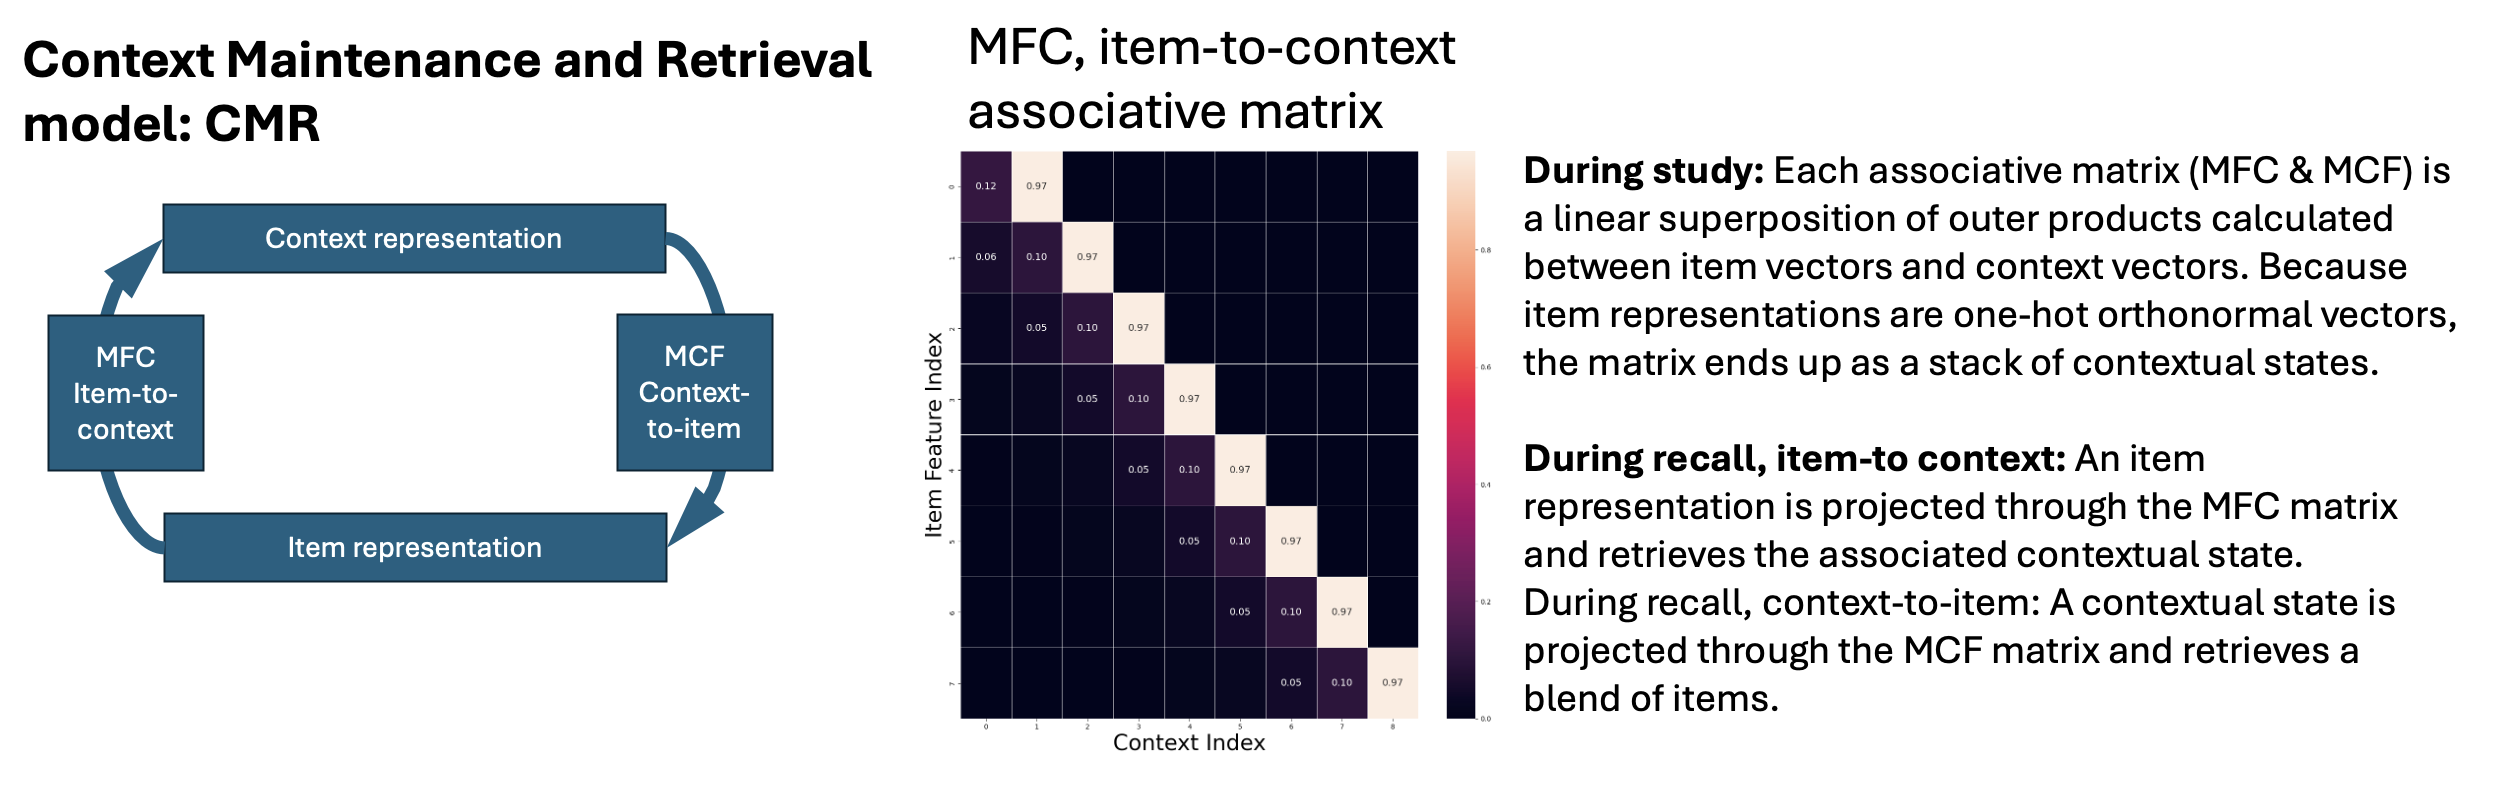
\includegraphics{icmr_figures/connectionistcmr_diagram.png}

}

\subcaption{\label{fig-connectionist-cmr}Connectionist CMR}

\end{minipage}%
\newline
\begin{minipage}{\linewidth}

\centering{

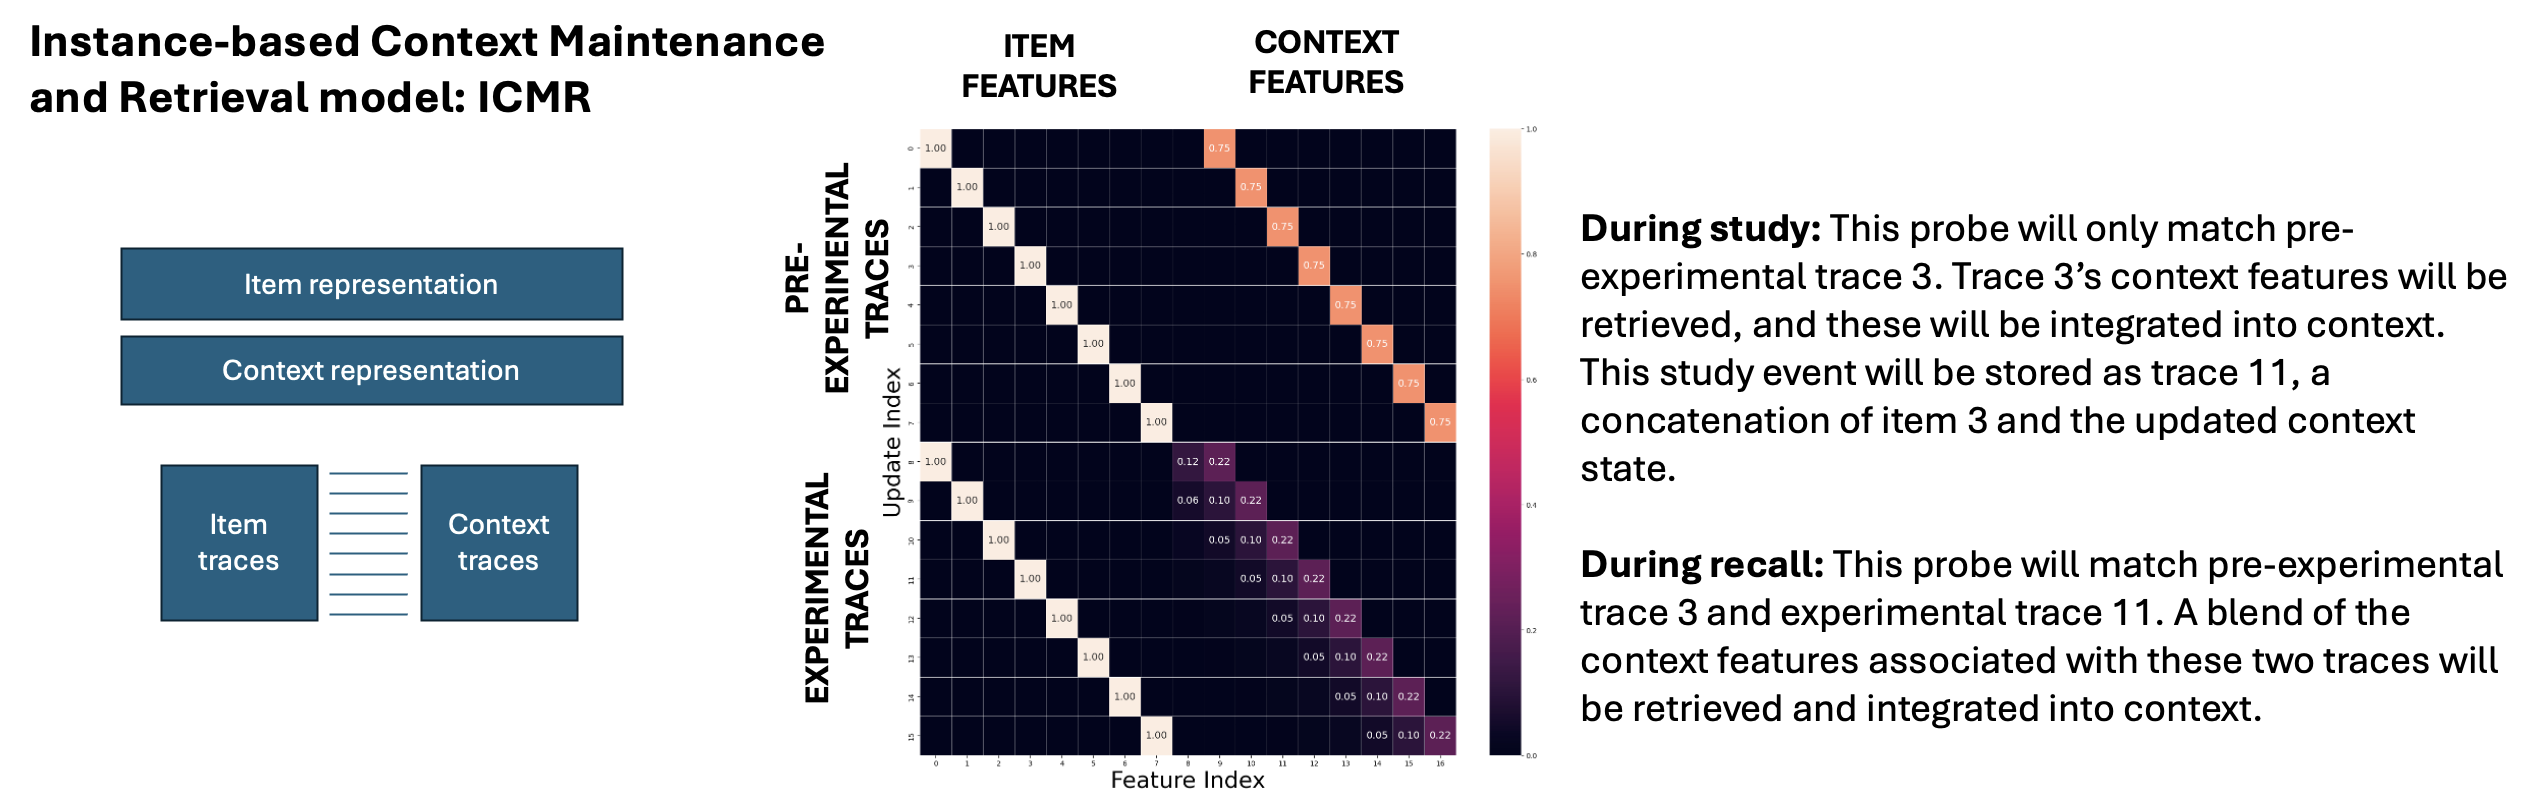
\includegraphics{icmr_figures/instancecmr_diagram.png}

}

\subcaption{\label{fig-instance-cmr}Instance CMR}

\end{minipage}%

\caption{\label{fig-comparison}\textbf{Aggregation of information across
memory traces happens at different time points in the two versions.} The
connectionist model aggregates over traces during encoding, because
there is a fixed-size set of associative weights. The instance model
creates separate traces for each event, so aggregation happens during
retrieval.}

\end{figure}%

We base our implementations of Connectionist CMR and Instance CMR on the
likelihood-based specification provided by Morton and Polyn (2016) and
Kragel, Morton, and Polyn (2015). The original connectionist version of
the Context Maintenance and Retrieval model (ConnectionistCMR) uses this
concept by employing two types of memory networks, \(M^{FC}\) and
\(M^{CF}\). These networks are linear associative networks where the
connection weights symbolize the forward and backward relationships
between the two layers. Essentially, these weights measure how strongly
specific items and contexts are linked based on how often they occur
together. In contrast, our initial specification of a multi-trace
version of CMR (InstanceCMR) also uses \(M^{FC}\) and \(M^{CF}\) to
represent the relationships between items and contexts. However, rather
than blending these associations into a cumulative pattern of weights,
each memory in Instance CMR keeps an individual trace for every
experience. This means it concatenates the states of \(F\) and \(C\) at
the time of encoding, preserving a distinct record for each event. To
fully explain how each model is structured, we first outline the memory
systems used by each model to encode and retrieve these item-context
associations. We then explore how both models manage these memories to
support the process of searching for memories and performing tasks like
free recall, where items must be remembered without prompts. This
comparison shows not just how the models store information but also how
they use it to reconstruct past events during memory tasks.

\begin{longtable}[]{@{}
  >{\raggedright\arraybackslash}p{(\columnwidth - 4\tabcolsep) * \real{0.2639}}
  >{\raggedright\arraybackslash}p{(\columnwidth - 4\tabcolsep) * \real{0.2639}}
  >{\raggedright\arraybackslash}p{(\columnwidth - 4\tabcolsep) * \real{0.4722}}@{}}
\caption{Parameters and structures specifying
CMR.}\label{tbl-cmr-parameters}\tabularnewline
\toprule\noalign{}
\begin{minipage}[b]{\linewidth}\raggedright
Symbol
\end{minipage} & \begin{minipage}[b]{\linewidth}\raggedright
Name
\end{minipage} & \begin{minipage}[b]{\linewidth}\raggedright
Description
\end{minipage} \\
\midrule\noalign{}
\endfirsthead
\toprule\noalign{}
\begin{minipage}[b]{\linewidth}\raggedright
Symbol
\end{minipage} & \begin{minipage}[b]{\linewidth}\raggedright
Name
\end{minipage} & \begin{minipage}[b]{\linewidth}\raggedright
Description
\end{minipage} \\
\midrule\noalign{}
\endhead
\bottomrule\noalign{}
\endlastfoot
\(C\) & temporal context & A recency-weighted average of encoded
items \\
\(F\) & item features & Current pattern of item feature unit
activations \\
\(M^{FC}\) & item-to-context memory & encoded feature-to-context
associations \\
\(M^{CF}\) & context-to-feature memory & encoded context-to-feature
associations \\
\({\beta}_{enc}\) & encoding drift rate & Rate of context drift during
item encoding \\
\({\beta}_{start}\) & start drift rate & Amount of start-list context
retrieved at start of recall \\
\({\beta}_{rec}\) & recall drift rate & Rate of context drift during
recall \\
\({\alpha}\) & shared support & Amount of support items initially have
for one another \\
\({\delta}\) & item support & Initial pre-experimental contextual
self-associations \\
\({\gamma}\) & learning rate & Amount of experimental context retrieved
by a recalled item \\
\({\phi}_{s}\) & primacy scale & Scaling of primacy gradient on trace
activations \\
\({\phi}_{d}\) & primacy decay & Rate of decay of primacy gradient \\
\({\theta}_{s}\) & stop probability scale & Scaling of the stop
probability over output position \\
\({\theta}_{r}\) & stop probability growth & Rate of increase in stop
probability over output position \\
\({\tau_{c}}\) & choice sensitivity & Exponential weighting of item
supports during the recall competition \\
\({\tau_{t}}\) & trace sensitivity & Exponential weighting of trace
activations during probes of \(M^{CF}\) \\
\end{longtable}

\subsection{Connectionist Memory
Representations}\label{connectionist-memory-representations}

In Connectionist CMR, the memories \(M^{FC}\) and \(M^{CF}\) are are
structured as two weight matrices, where each element is linked to the
features of items and contexts respectively. For example,
\(M^{FC}_{ij}\) represents the association between the \(i\)th feature
of an item and the \(j\)th context in feature-to-context memory
Figure~\ref{fig-connectionist-cmr}.

Before any experiment begins, we set up \(M^{FC}\) to summarize existing
associations between relevant item features and potential contextual
states. This initial configuration is guided by:

\begin{equation}\phantomsection\label{eq-1}{
M^{FC}_{pre(ij)} = \begin{cases} \begin{alignedat}{2} 1 - \gamma \text{, if } i=j \\\
          0 \text{, if } i \neq j
   \end{alignedat} \end{cases}
}\end{equation}

This setup connects each item feature unit on \(F\) to a unique context
unit on \(C\) using a parameter \(\gamma\), which dictates how much
pre-experimental associations influence the model's behavior.

Similarly, the associations from context to feature, managed by
\(M^{CF}\), are initially set as follows:

\begin{equation}\phantomsection\label{eq-2}{
M^{CF}_{pre(ij)} = \begin{cases} \begin{alignedat}{2} \delta \text{, if } i=j \\\
          \alpha \text{, if } i \neq j
       \end{alignedat} \end{cases}
}\end{equation}

Here, \(\delta\) adjusts the impact of pre-experimental
context-to-feature associations compared to those acquired during the
experiment. The \(\alpha\) parameter establishes a uniform semantic
support across items, supporting each other in the recall competition.

The weights between any two units \(i\) and \(j\) in \(M^{FC}\) or
\(M^{CF}\) are updated based on the Hebbian learning rule, which relies
on the activity levels in the item and context layers. Specifically, in
\(M^{FC}\), the learning rate of these updates is governed by the
\(\gamma\) parameter again:

\begin{equation}\phantomsection\label{eq-3}{
\Delta M^{FC}_{ij} = \gamma \cdot F_i \cdot C_j
}\end{equation}

This formula adjusts the strength of the connection based on the
simultaneous activity of item features \(F_i\) and context \(C_j\), with
the \(\gamma\) parameter controlling the learning rate.

In \(M^{CF}\), a function \(\phi\) enforces a primacy effect, scaling
the amount of learning based on the serial position of the studied item
according to:

\begin{equation}\phantomsection\label{eq-4}{ 
\phi_i = \phi_se^{-\phi_d(i-1)} + 1
}\end{equation}

where \(\phi_s\) and \(\phi_d\) are parameters that control the strength
and decay of the primacy effect, respectively.

The weight between units \(i\) and \(j\) in \(M^{CF}\) is updated
according to:

\begin{equation}\phantomsection\label{eq-5}{
\Delta M^{CF}_{ij} = \phi_i C_i F_j
}\end{equation}

To retrieve contextual associations for a given item, the model computes
the dot product of the item's feature vector \(f\) with \(M^{FC}\).

\begin{equation}\phantomsection\label{eq-6}{
\hat{C} = M^{FC} f
}\end{equation}

Similarly, to retrieve item associations for a given state of context,
the model computes the dot product of the context's feature vector \(c\)
with \(M^{CF}\).

\begin{equation}\phantomsection\label{eq-7}{
\hat{F} = M^{CF} c
}\end{equation}

These details describe how the connectionist CMR model encodes and
retrieves associations between items and contexts in memory and enforces
a primacy effect during learning to support memory search in the free
recall task.

\subsection{Instance-Based Memory
Representations}\label{instance-based-memory-representations}

In contrast to the traditional connectionist implementation of CMR, our
new instance-based specification of CMR (Instance CMR) represents
\(M^{FC}\) and \(M^{CF}\) as instance-based memories. That is, they
store a distinct trace for every experience, keeping each event's unique
details separate Figure~\ref{fig-instance-cmr}. Initially, like the
traditional model, Instance CMR uses two different memory matrices to
capture the associations between items and contexts (\(M^{FC}\) and
\(M^{CF}\)). This differentiation helps to account for differences in
how \(M^{FC}\) and \(M^{CF}\) represent pre-experimental associations
between item and context features. Later on, we will explore how merging
these into a single matrix that also incorporates semantic features can
streamline this process.

In the current specification, \(M^{FC}\) and \(M^{CF}\) are represented
as two multi-trace memories. Each trace is represented as a vector that
concatenates feature vectors representing the states of \(F\) and \(C\).
Each trace combines feature vectors from the item layer (\(F\)) and the
context layer (\(C\)), forming a complete snapshot of the encoding
event. These vectors are arranged in matrices where each row corresponds
to a different experience, and each column aligns with a particular
feature or context unit.

To ensure a clear comparison between the traditional composite and the
new multi-trace architectures, we initialize \(M^{FC}\) and \(M^{CF}\)
in Instance CMR to mirror the pre-experimental associations found in
Connectionist CMR. For \(M^{FC}\), this means setting up the memory with
a trace for each feature in \(F\) that connects to a specific context
unit in \(C\). Initially, all features in these traces are set to \(0\),
except for the ones directly linked, which are set to \(1\) and
\(1 - \gamma\) respectively.

Similarly, for \(M^{CF}\), each context unit in \(C\) starts connected
primarily to one feature in \(F\) but maintains a weaker link to all
other features. Here, context units in the traces are set to \(0\)
except for the primary connection, which is marked as \(1\). Item
features in these traces are mostly set to \(\alpha\), except for the
directly associated feature, which is initialized at \(\delta\). This
setup provides a structured foundation from which both memories can
evolve as they encode new experiences and interactions during the
experimental phase.

In the Instance CMR model, instead of updating a single weight between
units for each new experience, we add a new trace that captures the
state of both the item features \(F\) and the context features \(C\) at
the time of encoding. Differences in trace strengths (``learning rates''
in connectionist memories) are taken into account at retrieval rather
than encoding. So in \(M^{FC}\) and \(M^{CF}\) matrices, each experience
simply contributes a new trace that concatenates the item and context
feature vectors:

\begin{equation}\phantomsection\label{eq-8}{
M^{FC}_{exp_{i}} = [f_i, c_i]
}\end{equation}

\begin{equation}\phantomsection\label{eq-9}{
M^{CF}_{exp_{i}} = [c_i, f_i]
}\end{equation}

Retrieving associations from these multi-trace memories involves a
couple of steps. First, the probe vectors for \(M^{FC}\) consist only of
\(F\) features, formatted as \([f_{probe}, 0]\), and for \(M^{CF}\),
they consist only of context features, similarly formatted. These
vectors are concatenated with a zero vector to align with the
dimensionality of the traces in \(M^{FC}\) and \(M^{CF}\) . The
retrieval process then calculates a weighted sum across both
pre-experimental and experimental traces. The weight of each trace in
this sum is determined by the dot product between the probe vector and
the trace, as well as the trace's learning strength, which corresponds
to the learning rates in the connectionist models.

In the \(M^{FC}\) matrix, the parameter \(\gamma\) scales the
association between the item features and the contextual features within
these new traces; it's set to 1 for pre-experimental traces:

\begin{equation}\phantomsection\label{eq-10}{
[\hat{C} ...] = \sum_{i=1}^{n} \gamma M^{FC}_{i} [f, 0]
}\end{equation}

Similarly, in the \(M^{CF}\) matrix, the parameter \(\phi_{i}\) scales
the association of contextual features with the item features for each
new experience, where \(i\) is the index of an encoded trace and
\(\phi_i\) is held to 1 for pre-experimental traces:

\begin{equation}\phantomsection\label{eq-11}{
[\hat{F} ...] = \sum_{i=1}^{n} (\phi_i M^{CF}_{i} [c, 0] ]^{\tau_{t}}
}\end{equation}

For experimental traces, the equation defining \(\phi_i\) is the same as
described above for Connectionist CMR. However, the parameter \(\tau_t\)
is unique to the instance model. In \(M^{CF}\) (but not in \(M^{FC}\) ),
the parameter \(\tau_t\) is used to exponentiate the dot product between
the probe vector and each trace. This method enhances the difference in
activation between traces, allowing the most relevant or best-supported
traces to stand out more prominently during the retrieval process. This
feature, characteristic of instance models, accentuates the selectivity
of memory retrieval at the trace level. Since connectionist memories do
not support trace-level activation modulation in the same way, when
enforcing equivalence to Connectionist CMR, \(\tau_{t}\) is set to \(1\)
to effectively disable this mechanism and ensure that the model's
behavior is consistent with the connectionist specification.

\subsection{Memory Dynamics During the Free Recall
Task}\label{memory-dynamics-during-the-free-recall-task}

Remaining aspects of the model are shared between Connectionist and
Instance CMR.

\subsubsection{Encoding Phase}\label{encoding-phase}

When an item \(i\) is presented for study, its feature representation
\(f_i\) activates within the item layer \(F\), and its contextual
associations are retrieved from \(M^{FC}\), regardless of whether it's
the composite or multi-trace version. This retrieval modifies the
current state of the context layer \(C\). The input to the context from
this retrieval is defined by:

\begin{equation}\phantomsection\label{eq-12}{
c^{IN}_{i} = \hat{C}
}\end{equation}

Here, \(\hat{C}\) represents the context vector retrieved from
\(M^{FC}\). This vector is then normalized to maintain a consistent
scale, specifically so its length equals \(1\).

The context state is updated based on this input:

\begin{equation}\phantomsection\label{eq-13}{
c_i = \rho_i c_{i-1} + \beta_{enc} c_{i}^{IN}
}\end{equation}

In this formula, \(\beta_{enc}\) controls how much the context
changes--or drifts--with each new item presented, reflecting the
influence of the new contextual input. The parameter \(\rho\) is used to
ensure the length of \(c_i\) remains normalized at \(1\). It is
calculated as follows:

\begin{equation}\phantomsection\label{eq-14}{
\rho_i = \sqrt{1 + \beta^2\left[\left(c_{i-1} \cdot c^{IN}_i\right)^2 - 1\right]} - \beta\left(c_{i-1} \cdot c^{IN}_i\right)
}\end{equation}

This calculation adjusts \(\rho_i\) to balance the contribution of the
previous context state \(c_{i-1}\) and the new input \(c^{IN}_i\),
ensuring the overall context vector doesn't grow too large or become too
small.

At this point, the model captures and solidifies the association between
the current states of the context and item features in both \(M^{FC}\)
and \(M^{CF}\). This dynamic ensures that each new experience slightly
alters the context, which in turn influences how subsequent items are
encoded and later retrieved.

\subsubsection{Retrieval Phase}\label{retrieval-phase}

To account for the primacy effect in the model, we posit that between
the encoding and retrieval phases, the content of the context layer
\(C\) drifts back towards its state prior to the experiment. We model
this drift and set the initial state of context at the start of
retrieval as follows, with \(\rho\) calculated as previously specified:

\begin{equation}\phantomsection\label{eq-15}{
c_{start} = \rho_{N+1}c_N + \beta_{start}c_0
}\end{equation}

During each recall attempt, this current state of context serves as the
cue to \(M^{CF}\), attempting to retrieve a studied item and producing
an activation vector A on the item layer \(F\):

\begin{equation}\phantomsection\label{eq-155}{
A = \hat{F}
}\end{equation}

To ensure all items have a chance of being recalled, each is given a
baseline activation of \(10^{-7}\). The likelihood of ending the recall
session, or the probability of stopping the recall without retrieving
any more items, depends on the output position \(j\) and is given by:

\begin{equation}\phantomsection\label{eq-16}{
P(stop, j) = \theta_s e^{j\theta_r}
}\end{equation}

Here, \(\theta_s\) and \(\theta_r\) govern the initial stopping
probability and the rate at which this probability increases,
respectively, which is modeled as an exponential function. If recall
continues, the probability \(P(i)\) of recalling a specific item \(i\)
primarily depends on its relative activation strength:

\begin{equation}\phantomsection\label{eq-17}{
P(i) = (1-P(stop))\frac{A^{\tau_{c}}_i}{\sum_{k}^{N}A^{\tau_{c}}_k}
}\end{equation}

The parameter \(\tau_{c}\) enhances the contrast in activation strengths
between items: a high \(\tau_{c}\) value amplifies differences, making
the most activated item even more likely to be recalled, whereas a lower
\(\tau_{c}\) value diminishes these differences, equalizing recall
probabilities across items with varying activations. This mechanism can
be implemented for either instance-based or connectionist memories, even
on top of pre-existing trace-based activation scaling.

If an item is recalled, it is reactivated on \(F\), and its contextual
associations are retrieved to update the context. This new context input
is:

\begin{equation}\phantomsection\label{eq-18}{
c^{IN}_{i} = \hat{C}
}\end{equation}

Context is then updated based on this input using \(\beta_{rec}\) (used
during retrieval rather than encoding) to adjust for the current phase
of the task, setting the stage for the next recall attempt. This
iterative process continues until no further items are recalled,
effectively concluding the recall session.

\section{Simulation 1: Functional Equivalence Between Connectionist and
Instance
CMR}\label{simulation-1-functional-equivalence-between-connectionist-and-instance-cmr}

We have established two versions of the Context Maintenance and
Retrieval model: Connectionist CMR and Instance CMR that both
instantiate the principles of retrieved context theory to explain memory
search in free recall tasks. But are the models truly equivalent, or are
there subtle differences in their behavior that could influence their
performance in different scenarios? While we hold the trace-based
activation scaling parameter \(\tau_{t}\) constant at 1, the answer to
this question is yes. The reason why is that the two models use the same
feature and contextual representations, and perform the same
mathematical operations upon them to encode and retrieve associations:
The pre-scaled activation of an output feature in either model is
determined by the dot product similarity between probe vectors and
output features' associated input features, weighted by each trace's
respective learning rate. Here we present simulation analyses of the
functional equivalence between Connectionist CMR and Instance CMR,
demonstrating how both models encode and retrieve the same associations
despite their structural differences. Establishing the equivalence of
Instance CMR and Connectionist CMR under these conditions allows us to
explore how trace-based activation scaling might enhance the model's
performance in free recall tasks.

To clarify the roles of memory structures in the simulation of CMR and
underscore how these models encode and retrieve the same associations
despite their structural differences, we provide a functional analysis
of the connectivity structure of \(M^{FC}\) and \(M^{CF}\) in both
models that measures associations between item and context features
irrespective of how these associations are represented within a memory
architecture. To set up this analysis, we use parameters fitted to the
subset of the PEERS dataset as reported by (Healey and Kahana 2014) as
described in the next section, but with \(\tau_{t}\) set to 1. Then we
simulate encoding of an arbitrary study list of size 8 with each model
to construct the memory structures \(M^{FC}\) and \(M^{CF}\) that would
organize retrieval in a free recall task.

To compare the connectivity matrices of Connectionist CMR and Instance
CMR, we individually activate each input unit and measure the resulting
activation in the output layer for each possible input unit, activating
one unit at a time. The resulting vector represents the connectivity
between the activated input unit and all output units. Stacking these
vectors together, we obtain the full latent connectivity matrix for each
memory structure. For connectionist \(M^{FC}\) and \(M^{CF}\), this
extracted structure is identical to the weight matrices used in the
model. But for instance-based \(M^{FC}\) and \(M^{CF}\), this structure
is effectively a conversion of the multi-trace memory into a composite
memory, where each row summarizes associations between an input unit and
all output units across all study events.

Along with producing latent \(M^{FC}\) and \(M^{CF}\) connectivity
matrices, we also analyze their combined influence on the dynamics of
memory search in free recall tasks by extracting a latent \(M^{FF}\)
matrix that passes \(F\) input vectors through \(M^{FC}\) and then
passes the resulting context vectors through \(M^{CF}\) to measure the
strength of associations between item features across all study events.
This matrix reflects the interplay between \(M^{FC}\) and \(M^{CF}\) in
guiding memory search -- how recalling an item will bias the retrieval
of subsequent items based on the context reinstated by the recalled item
via \(M^{FC}\) and then used as a retrieval cue via \(M^{CF}\). In
Figure~\ref{fig-matrix}, we illustrate that across Connectionist CMR and
Instance CMR, these three latent connectivity structures are identical,
despite the differences in how they store and retrieve associations.

To further illustrate how the memory structures of Connectionist CMR and
Instance CMR support the temporal organization of memory search, we
analyze extracted latent connectivity matrices from both models in a
lag-connectivity analysis. In latent \(M^{FC}\) representations, this
analysis measures the connection strength between each considered item's
\(F\) representations with each other item's pre-experimentally
associated context units \(C\) as a function of the other items' serial
lag from the considered item. The connection weight between \(F_i\) and
\(C_j\) for all items \(i\) and \(j\) is calculated for each lag \(j-i\)
and plotted as a function of this lag. For example, if item \(i\) is
considered, the lag-connectivity analysis measures the strength of the
connection between \(F_i\) and \(C_j\) as a function of the lag \(j-i\).
A converse analysis is performed for \(M^{CF}\), measuring the
connection strength between each considered context unit \(C_i\) with
each other item's pre-experimentally associated feature units \(F\) as a
function of the other items' serial lag from the considered item.

Finally, to measure the combined influence of \(M^{FC}\) and \(M^{CF}\)
on memory search, we perform a lag-connectivity analysis on the latent
\(M^{FF}\) matrix, measuring the connection strength between each
considered item's \(F\) representations with each other item's \(F\)
representations as a function of the other items' serial lag from the
considered item. This analysis, visualized in
Figure~\ref{fig-lag-connectivity}, provides a visual representation of
how each of \(M^{FC}\) and \(M^{CF}\) supports the lag-contiguity effect
in free recall tasks, with \(M^{FC}\) primarily supporting transitions
to backward neighbors of the last recalled item and \(M^{CF}\)
supporting transitions to forward neighbors. The analysis applied to
\(M^{FF}\) demonstrates how the combined influence of \(M^{FC}\) and
\(M^{CF}\) instantiates a bidirectional but forward-biased
lag-connectivity structure that supports the assymetrical lag-contiguity
effect in free recall tasks. These analyses together demonstrate that
the latent connectivity structures of Connectionist CMR and Instance CMR
are functionally equivalent, supporting the same dynamics of memory
search in free recall tasks.

\begin{figure}

\begin{minipage}{0.50\linewidth}
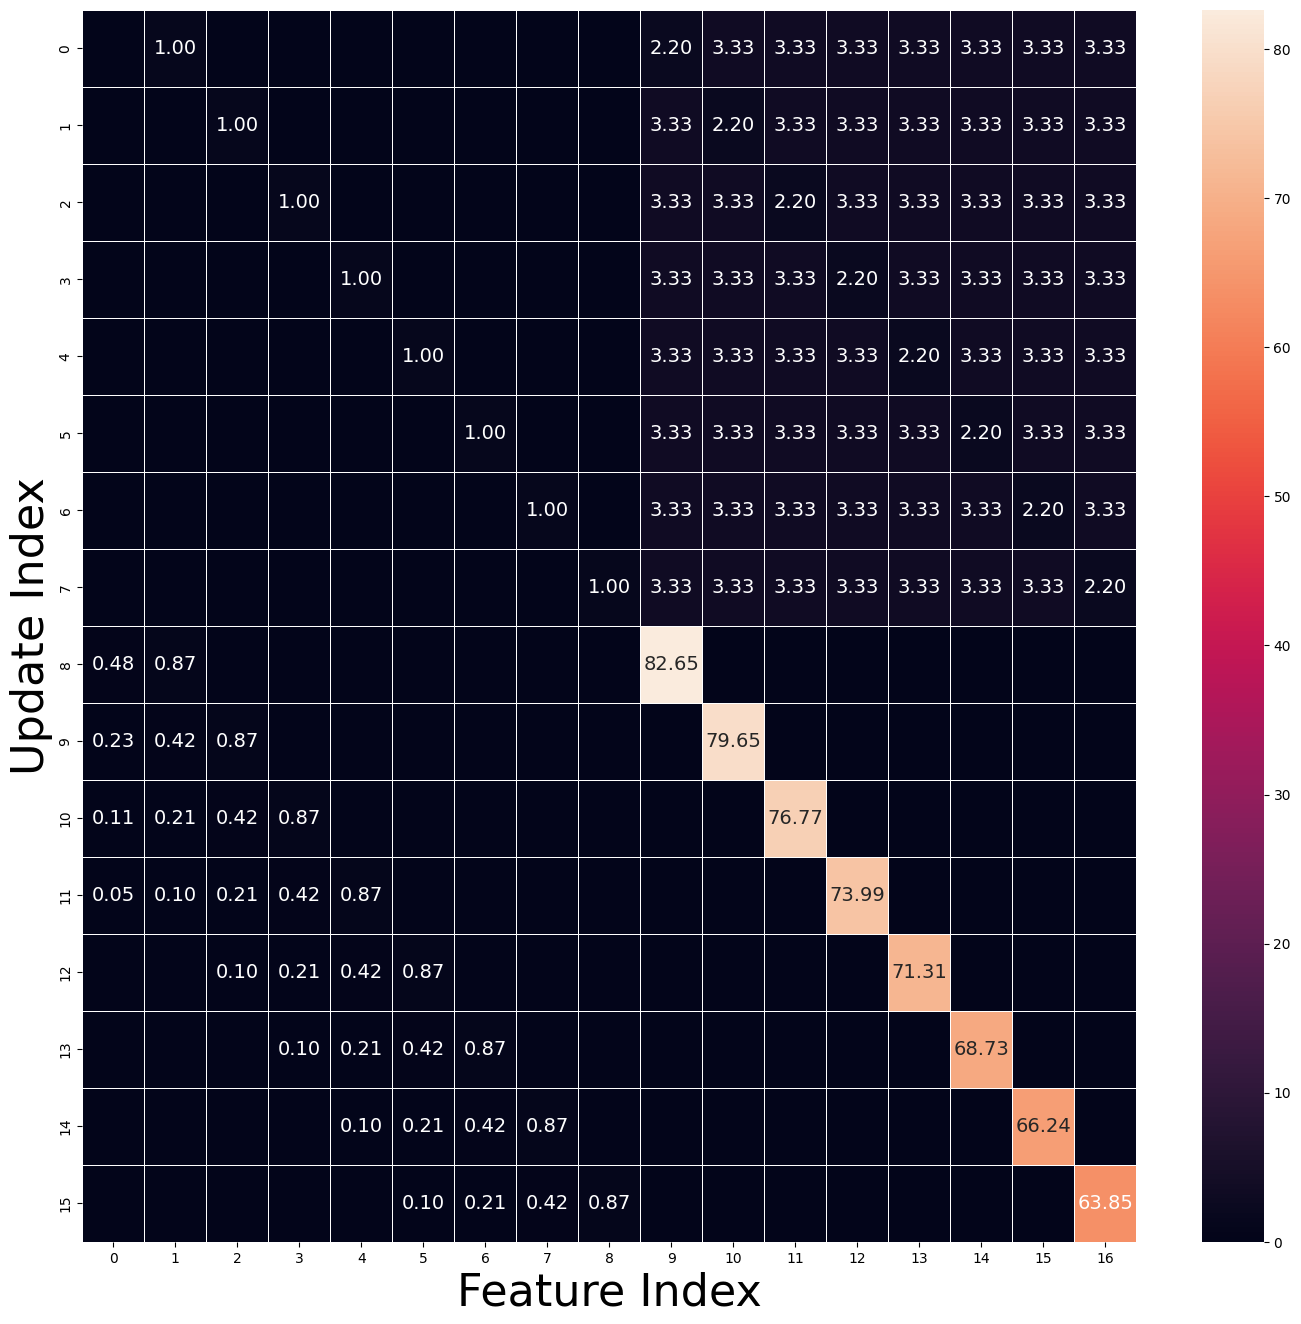
\includegraphics{icmr_figures/icmr_mfc.png}\end{minipage}%
%
\begin{minipage}{0.50\linewidth}
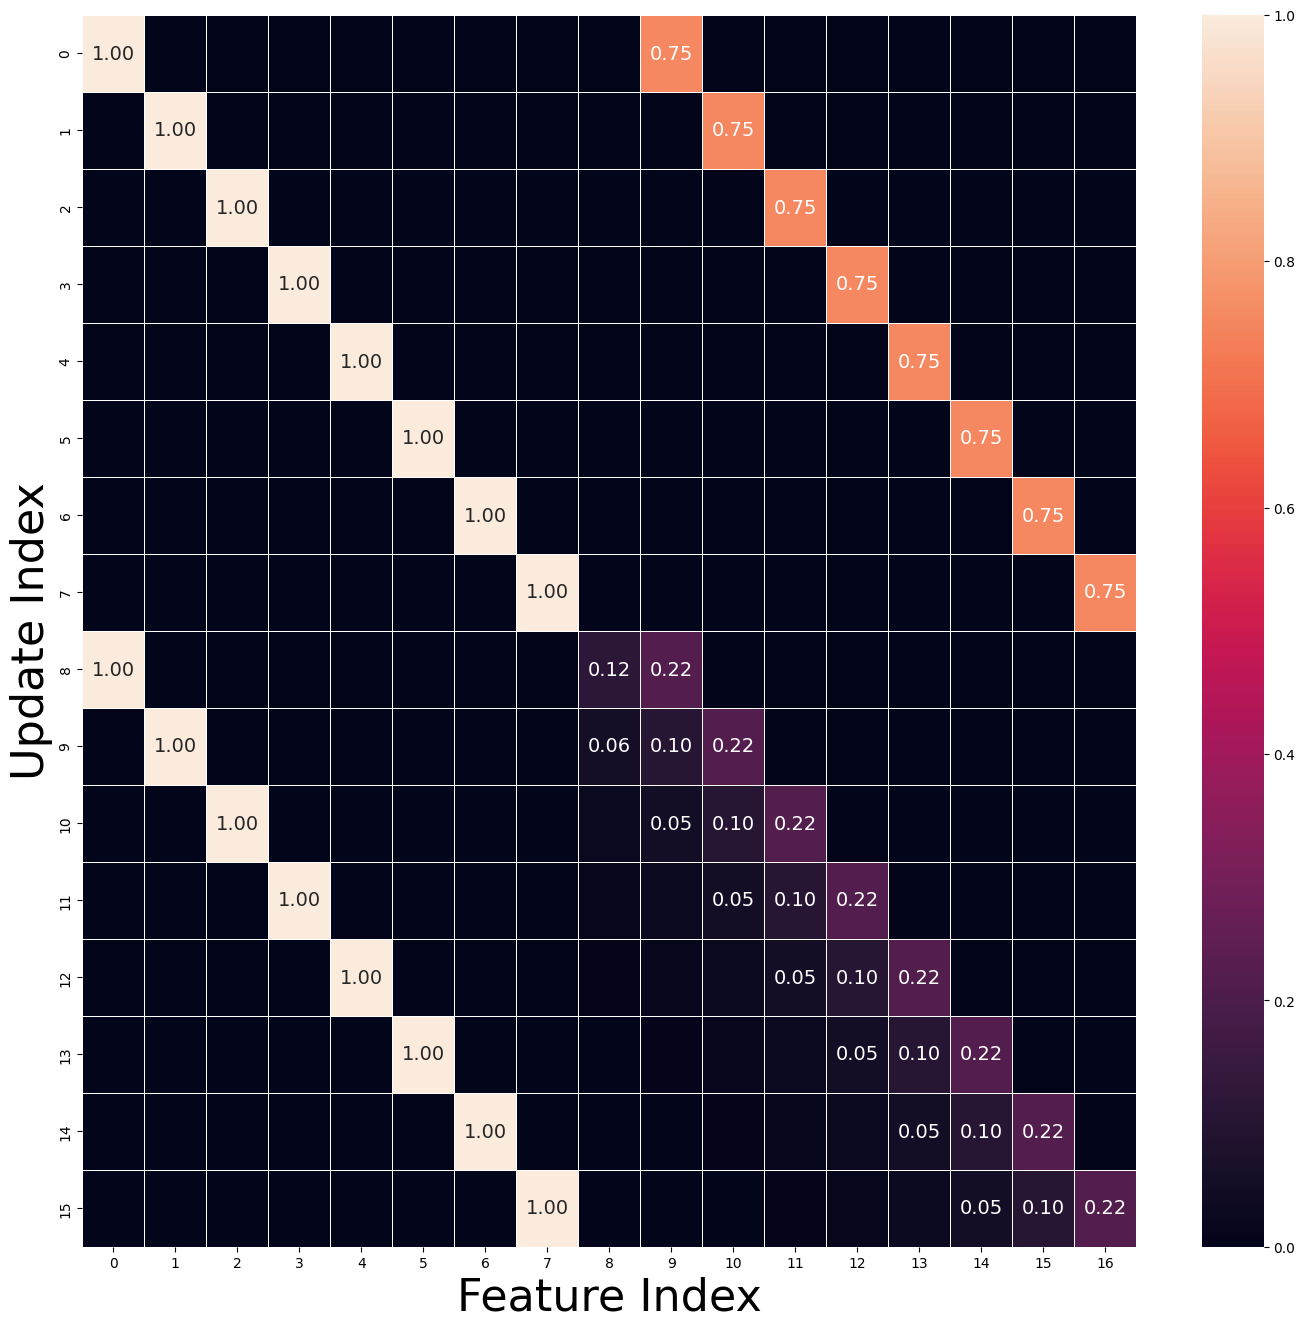
\includegraphics{icmr_figures/icmr_mcf.png}\end{minipage}%
\newline
\begin{minipage}{0.33\linewidth}
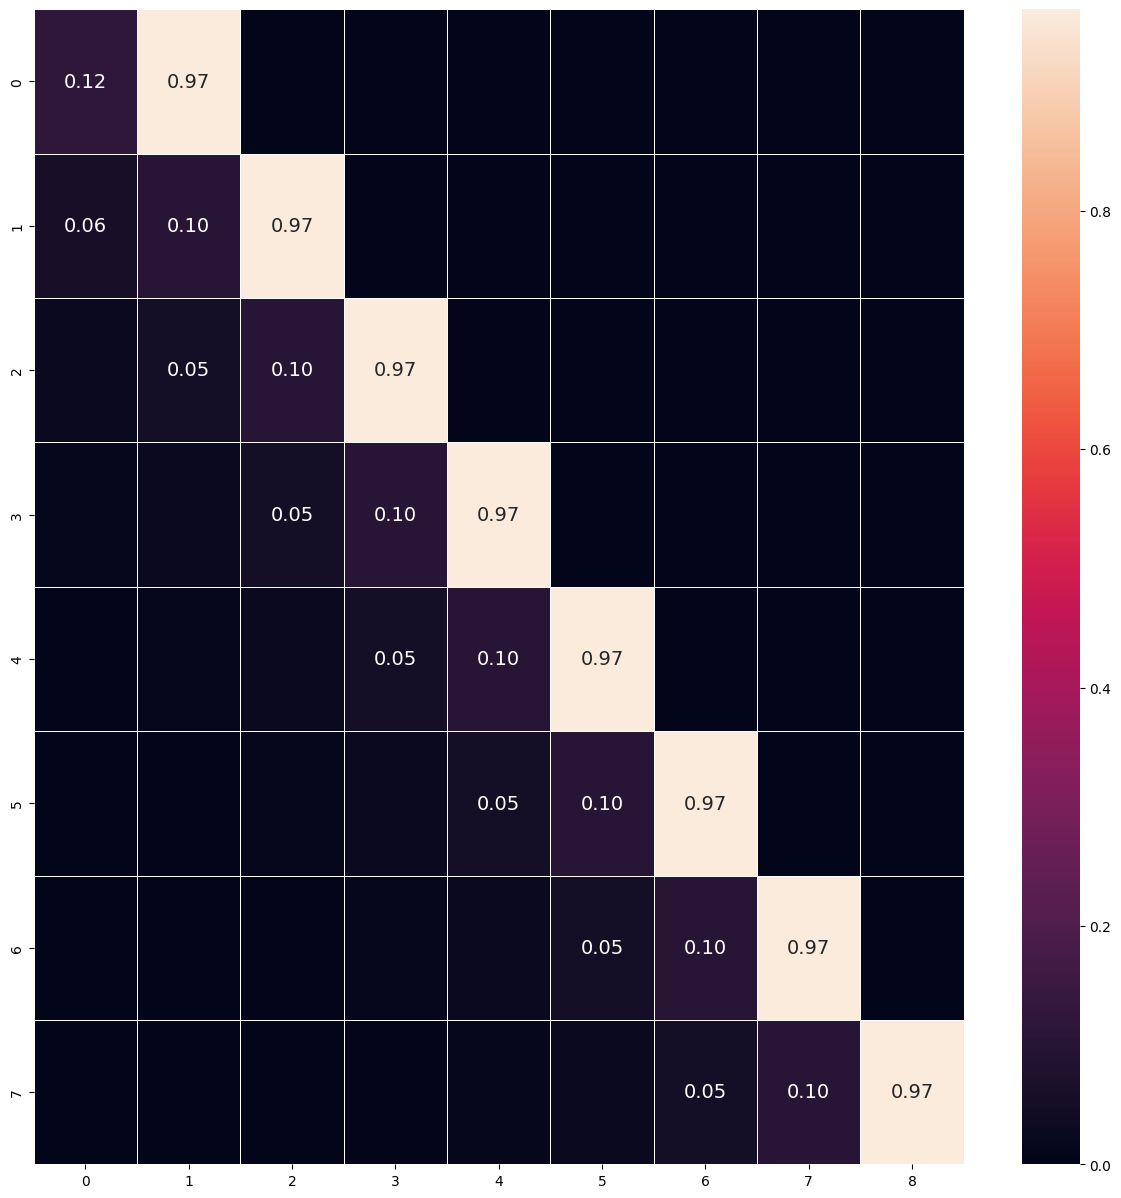
\includegraphics{icmr_figures/latent_mfc.png}\end{minipage}%
%
\begin{minipage}{0.33\linewidth}
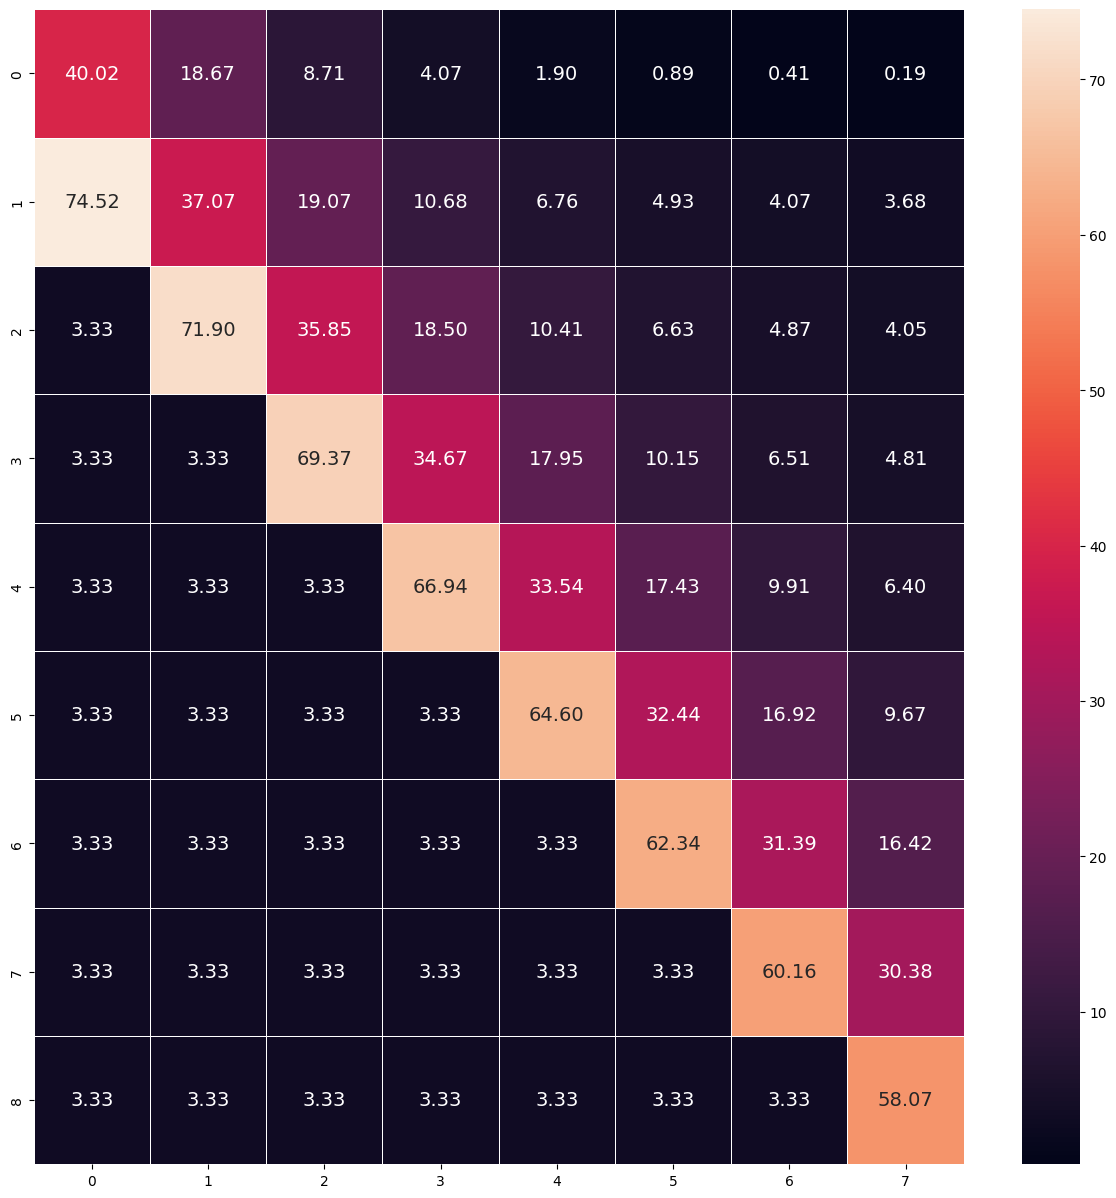
\includegraphics{icmr_figures/latent_mcf.png}\end{minipage}%
%
\begin{minipage}{0.33\linewidth}
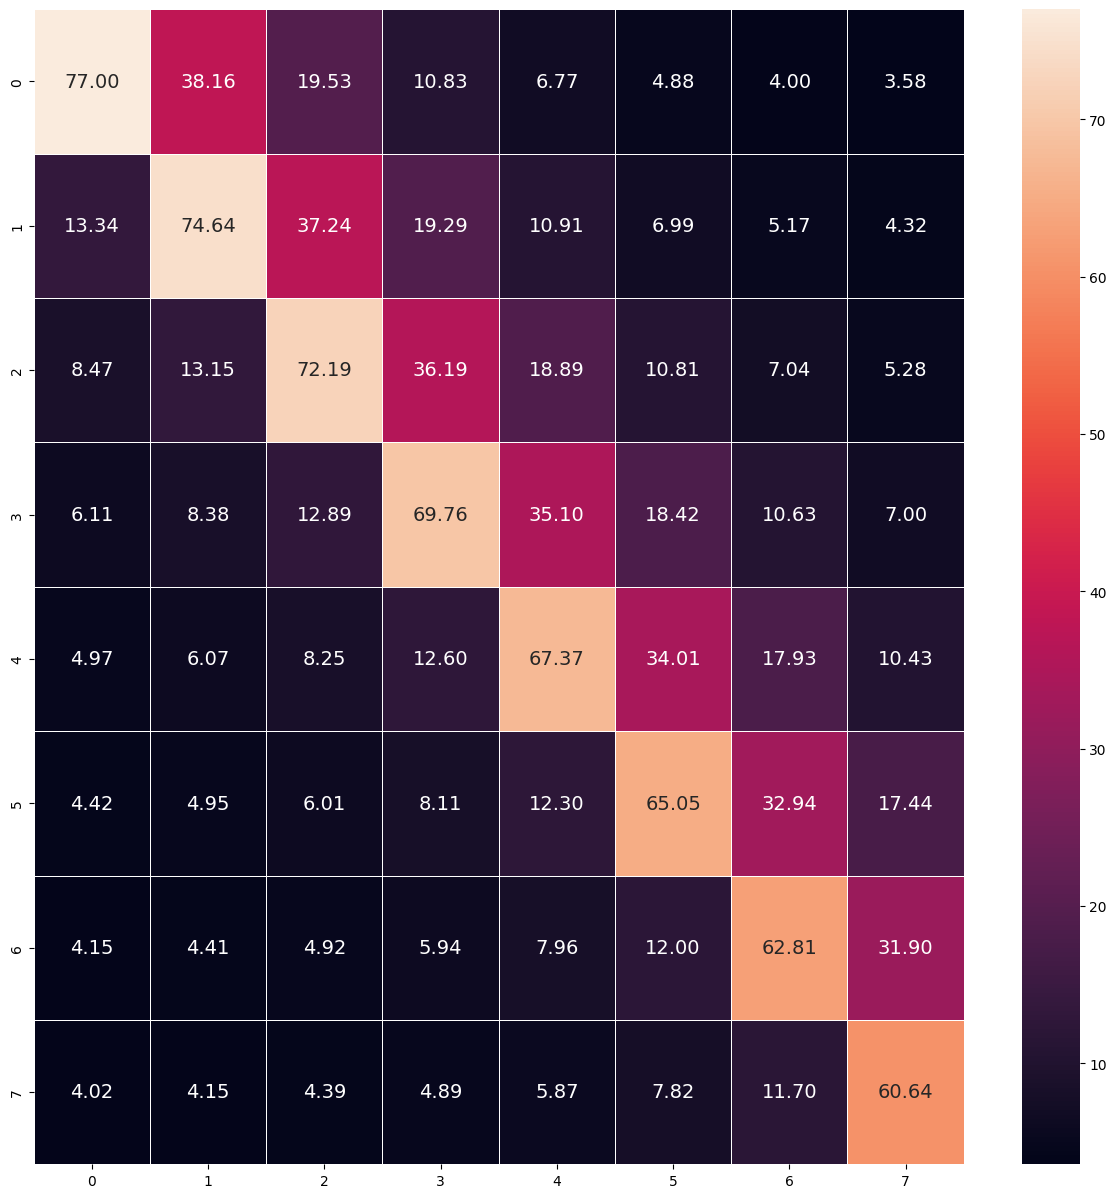
\includegraphics{icmr_figures/latent_mff.png}\end{minipage}%

\caption{\label{fig-matrix}\textbf{Comparison of latent connectivity
matrices between Connectionist CMR and Instance CMR}. Top Row: Instance
CMR's \(M^{FC}\) (left), and \(M^{CF}\) (right) matrices. Each row
represents a memory trace associating item and context features. Bottom
Row: Extracted latent connectivity matrices from either CMR variant's
\(M^{FC}\) (left), and \(M^{CF}\) (middle) memories as well as the
combined influence of \(M^{FC}\) and \(M^{CF}\) on memory search in the
\(M^{FF}\) matrix (right). These are identical between the Instance and
Connectionist models and also identical to Connectionist CMR's
\(M^{FC}\) and \(M^{CF}\) weight matrices.}

\end{figure}%

\begin{figure}

\begin{minipage}{0.33\linewidth}
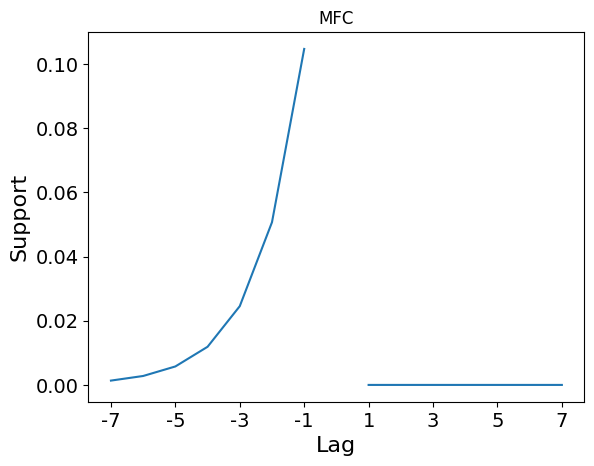
\includegraphics{icmr_figures/mfc_lag_connectivity.png}\end{minipage}%
%
\begin{minipage}{0.33\linewidth}
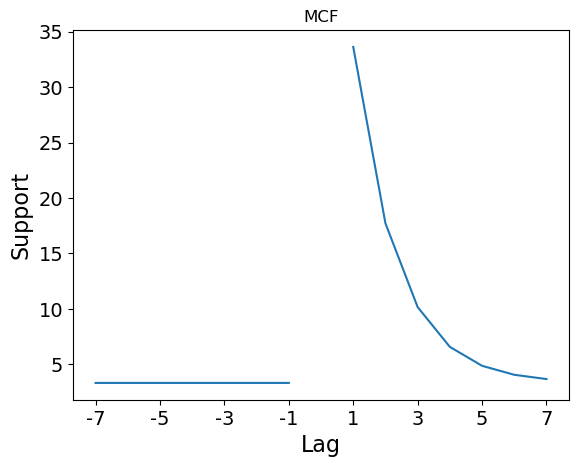
\includegraphics{icmr_figures/mcf_lag_connectivity.png}\end{minipage}%
%
\begin{minipage}{0.33\linewidth}
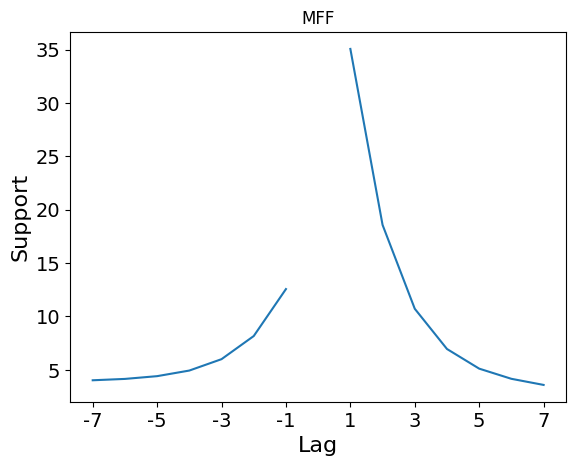
\includegraphics{icmr_figures/mff_lag_connectivity.png}\end{minipage}%

\caption{\label{fig-lag-connectivity}\textbf{Lag-connectivity analysis
of latent connectivity matrices} from \(M^{FC}\) (left), \(M^{CF}\)
(middle), and \(M^{FF}\) (right) in both models. These analyses show how
each memory structure supports the lag-contiguity effect in free recall
tasks.}

\end{figure}%

\section{Simulation 2: Performance of Connectionist and Instance CMR on
Free Recall
Datasets}\label{simulation-2-performance-of-connectionist-and-instance-cmr-on-free-recall-datasets}

As shown, in our specification, Connectionist and Instance CMR models
are functionally equivalent when the trace-based activation scaling
parameter \(\tau_{t}\) is set to 1. This setup ensures that with
identical parameter configurations, both models should yield the same
results in free recall tasks. This equivalence is maintained by using
consistent association encodings between item and context features,
identical learning rates, primacy scaling parameters across experiences,
and by disabling the trace-based activation scaling in the instance
model. To demonstrate how both models equivalently handle the dynamics
of memory search in free recall, we simulate their performance on a
selection of free recall datasets previously used to assess the
Connectionist CMR, as well as exploring how Instance CMR performs when
\(\tau_{t}\) is varied during model fitting. This will help determine
the potential benefits of trace-based activation scaling in these tasks.

\subsection{Datasets}\label{datasets}

For our initial comparisons, we utilize a segment of the PEERS dataset
as reported by (Healey and Kahana 2014). In this subset, each of 126
participants, aged 17 to 30, encountered 112 trials where they studied
lists of 16 unique words, followed by immediate recall. The words in
each trial were unique and selected for low similarity, randomly drawn
from the Toronto Word Pool (Friendly et al. 1982), which includes
high-frequency nouns, adjectives, and verbs.

One significant aspect of the CMR model is its ability to demonstrate
the relative scale-invariance of serial position effects, regardless of
list length. As documented by (Murdock Jr 1962), variations in list
length did not affect the primacy or the shape of the recency effects
observed, though they did influence the overall probability of recalling
initially encoded items and the list-list asymptote. To assess whether
our multi-trace and composite implementations of CMR can replicate these
findings, we utilize a subset of the original behavioral data from
(Murdock Jr 1962) where 15 subjects completed 240 trials with list
lengths varying between 20, 30, and 40 words.

Additionally, past research (L. Lohnas and Kahana 2014) has highlighted
CMR's capacity to model various repetition effects observed in free
recall experiments. N otably, recall sequences often show a spacing
effect, where the likelihood of recalling an item increases with the lag
between its repeated presentations in a study list. (L. Lohnas and
Kahana 2014) demonstrated that CMR could account for this through two
mechanisms: contextual variability and study-phase retrieval. In the
study-phase retrieval, when an item appears multiple times, recalling
its prior instances and their contexts enriches the associations made
with the current presentation. We test our model implementations against
the dataset from (L. Lohnas and Kahana 2014), where 35 subjects recalled
48 lists over four sessions. Each session included unique words, with
controlled semantic relatedness below a threshold of .55 according to
WAS (Steyvers, Shiffrin, and Nelson 2005), and featured four types of
list structures:

\begin{enumerate}
\def\labelenumi{\arabic{enumi}.}
\tightlist
\item
  \textbf{Control lists}: Each item appeared only once.
\item
  \textbf{Pure massed lists}: Items appeared twice consecutively (e.g.,
  1, 1, 2, 2).
\item
  \textbf{Pure spaced lists}: Items appeared twice with variable
  spacings from 1 to 8 positions.
\item
  \textbf{Mixed lists}: Contained once-presented, massed, and spaced
  items, with each spacing amount distributed equally.
\end{enumerate}

Through these simulations, we aim to further understand how different
memory model architectures influence recall dynamics and whether certain
features, like trace-based activation scaling, enhance the model's
predictive accuracy and applicability across varied recall scenarios.

\subsection{Likelihood-based model optimization and
comparison}\label{likelihood-based-model-optimization-and-comparison}

To determine how accurately each model captures the sequence of items
recalled in our experiments, we employ a likelihood-based model
comparison technique, as suggested by Kragel, Morton, and Polyn (2015).
This method evaluates model variants based on their precision in
predicting the exact order of recalled items. According to this method,
repeated items and intrusions (responses naming items not presented in
the list) are excluded from participants' recall sequences.

Here's how it works: For each trial, after simulating the encoding of
each item as presented in the study list, the model begins by predicting
the likelihood of the first item recalled by the participant.
Subsequently, the model simulates the retrieval of this item, updates
its state, and uses this updated context to predict the next recall
event---this could either be the retrieval of another item or the
termination of the recall session. This process continues until no
further items are recalled. The probability assigned by the model to
each recall event, conditional on prior events in the sequence, is
recorded, log-transformed, and summed to derive the log-likelihood for
the entire sequence. Across multiple trials in a dataset, these sequence
log-likelihoods are summed to calculate the total log-likelihood for the
dataset under a given model and parameter set. Higher log-likelihoods
indicate a model's superior capability to account for the observed data.

Optimizing the parameters for each model to maximize the likelihood of
the observed data is achieved using the differential evolution technique
(Storn and Price 1997), implemented in the scipy Python library. This
method involves maintaining a population of potential parameter
configurations. In each iteration, the algorithm mutates each member of
this population by combining them with other members in a stochastic
manner. If the new configuration offers an improvement, it replaces the
older one; otherwise, it is discarded. This iterative process helps in
progressively refining the parameters until they converge on a
configuration that maximizes the observed dataset's log-likelihood. We
conduct optimization at the individual subject level and compare models
by examining the distribution of log-likelihood values across subjects,
which helps in identifying the most effective model configuration for
explaining recall dynamics.

\subsection{Summary Statistic
Simulation}\label{summary-statistic-simulation}

In our evaluations of model performance, we utilize a set of summary
statistics to characterize recall sequences. To calculate these
statistics for the models, we first simulate recall sequences based on
the specified model mechanics. For each unique study list in our
dataset, we simulate 1000 trials. Each trial involves simulating the
encoding of each item into memory followed by the stochastic simulation
of free recall, which continues according to the calculated
probabilities for each recall attempt until the session ends. The
summary statistics for each model are then computed across all these
simulations.

Our analysis primarily focuses on four well-documented regularities in
free recall tasks that significantly influence model evaluation:

\begin{enumerate}
\def\labelenumi{\arabic{enumi}.}
\tightlist
\item
  \textbf{Serial Position Effect}: This effect is crucial for
  understanding how the order of items in a study list affects their
  likelihood of recall. We calculate and visualize the retrieval rate
  for each item based on its position in the study list. The rates for
  items presented early in the list help quantify the primacy effect,
  while the retrieval rates for later items illustrate the recency
  effect.
\item
  \textbf{Probability of First Recall}: This statistic measures the rate
  at which items are retrieved first across recall sequences. This
  metric helps identify the items that are most likely to initiate the
  recall process.
\item
  \textbf{Lag-Contiguity Effect}: This phenomenon, where items close
  together in the list order tend to be recalled in close sequence, is
  another focal point of our analysis. To assess this, we employ
  lag-based conditional response probability (lag-CRP) analyses. The
  ``lag'' here refers to the distance between two items in the study
  list. We calculate the probability of a participant or model making a
  transition to recall an item at a specific lag, given that such a
  transition is possible. A high degree of temporal contiguity is
  indicated by frequent transitions to nearby items and infrequent
  transitions to items further apart.
\item
  \textbf{Spacing Effect}: The spacing effect describes how the
  intervals between item presentations within a study list influence
  recall probability. We plot the probability of recalling an item based
  on its lag from the last presentation (or whether it is a novel item).
  This analysis helps us understand how the model's memory dynamics are
  influenced by the spacing between repeated items.
\end{enumerate}

We plot simulated data against observed data to evaluate how well the
models capture these regularities across different datasets.

\subsection{Results}\label{results}

\subsubsection{Healey \& Kahana (2014)}\label{healey-kahana-2014}

\begin{longtable}[]{@{}
  >{\raggedright\arraybackslash}p{(\columnwidth - 10\tabcolsep) * \real{0.2800}}
  >{\raggedright\arraybackslash}p{(\columnwidth - 10\tabcolsep) * \real{0.1400}}
  >{\raggedright\arraybackslash}p{(\columnwidth - 10\tabcolsep) * \real{0.1400}}
  >{\raggedright\arraybackslash}p{(\columnwidth - 10\tabcolsep) * \real{0.1400}}
  >{\raggedright\arraybackslash}p{(\columnwidth - 10\tabcolsep) * \real{0.1400}}
  >{\raggedright\arraybackslash}p{(\columnwidth - 10\tabcolsep) * \real{0.1400}}@{}}
\caption{Confidence intervals of parameters fit to data from Healey and
Kahana (2014), computed across subjects. Column 1: Connectionist CMR
follows the specification in Morton and Polyn (2016). Column 2: Instance
CMR with \(\tau_{t}\) set to 1. Column 3: Instance CMR with \(\tau_{t}\)
optimized during fitting but \(\tau_{c}\) set to 1. Column 4: Instance
CMR with both \(\tau_{t}\) and \(\tau_{c}\) optimized during fitting.
}\label{tbl-healey}\tabularnewline
\toprule\noalign{}
\begin{minipage}[b]{\linewidth}\raggedright
\end{minipage} & \begin{minipage}[b]{\linewidth}\raggedright
Connectionist CMR
\end{minipage} & \begin{minipage}[b]{\linewidth}\raggedright
Instance CMR
\end{minipage} & \begin{minipage}[b]{\linewidth}\raggedright
Trace Scaling CMR
\end{minipage} & \begin{minipage}[b]{\linewidth}\raggedright
Multi Scaling CMR
\end{minipage} & \begin{minipage}[b]{\linewidth}\raggedright
\end{minipage} \\
\midrule\noalign{}
\endfirsthead
\toprule\noalign{}
\begin{minipage}[b]{\linewidth}\raggedright
\end{minipage} & \begin{minipage}[b]{\linewidth}\raggedright
Connectionist CMR
\end{minipage} & \begin{minipage}[b]{\linewidth}\raggedright
Instance CMR
\end{minipage} & \begin{minipage}[b]{\linewidth}\raggedright
Trace Scaling CMR
\end{minipage} & \begin{minipage}[b]{\linewidth}\raggedright
Multi Scaling CMR
\end{minipage} & \begin{minipage}[b]{\linewidth}\raggedright
\end{minipage} \\
\midrule\noalign{}
\endhead
\bottomrule\noalign{}
\endlastfoot
fitness & 590.11 +/- 16.87 & 589.14 +/- 16.92 & 589.04 +/- 16.87 &
588.32 +/- 16.97 & \\
encoding drift rate & 0.79 +/- 0.02 & 0.80 +/- 0.02 & 0.75 +/- 0.03 &
0.71 +/- 0.04 & \\
start drift rate & 0.29 +/- 0.04 & 0.27 +/- 0.04 & 0.23 +/- 0.04 & 0.26
+/- 0.04 & \\
recall drift rate & 0.85 +/- 0.02 & 0.85 +/- 0.02 & 0.89 +/- 0.02 & 0.88
+/- 0.02 & \\
shared support & 22.73 +/- 5.26 & 23.83 +/- 5.51 & 0.14 +/- 0.07 & 25.02
+/- 5.08 & \\
item support & 22.68 +/- 4.65 & 26.20 +/- 5.16 & 22.82 +/- 5.19 & 28.25
+/- 5.30 & \\
learning rate & 0.49 +/- 0.06 & 0.49 +/- 0.06 & 0.33 +/- 0.04 & 0.51 +/-
0.06 & \\
primacy scale & 25.59 +/- 5.55 & 30.50 +/- 5.78 & 48.46 +/- 5.80 & 10.24
+/- 3.53 & \\
primacy decay & 10.53 +/- 4.42 & 14.09 +/- 4.96 & 10.78 +/- 3.75 & 15.66
+/- 4.41 & \\
stop probability scale & 0.01 +/- 0.00 & 0.01 +/- 0.00 & 0.01 +/- 0.00 &
0.01 +/- 0.00 & \\
stop probability growth & 0.40 +/- 0.02 & 0.40 +/- 0.02 & 0.40 +/- 0.02
& 0.40 +/- 0.02 & \\
choice sensitivity & 38.70 +/- 6.24 & 31.31 +/- 5.55 & 1.00 +/- 0.00 &
48.98 +/- 6.09 & \\
mcf trace sensitivity & 1.00 +/- 0.00 & 1.00 +/- 0.00 & 2.87 +/- 0.26 &
2.02 +/- 0.28 & \\
\end{longtable}

\begin{figure}

\begin{minipage}{0.33\linewidth}
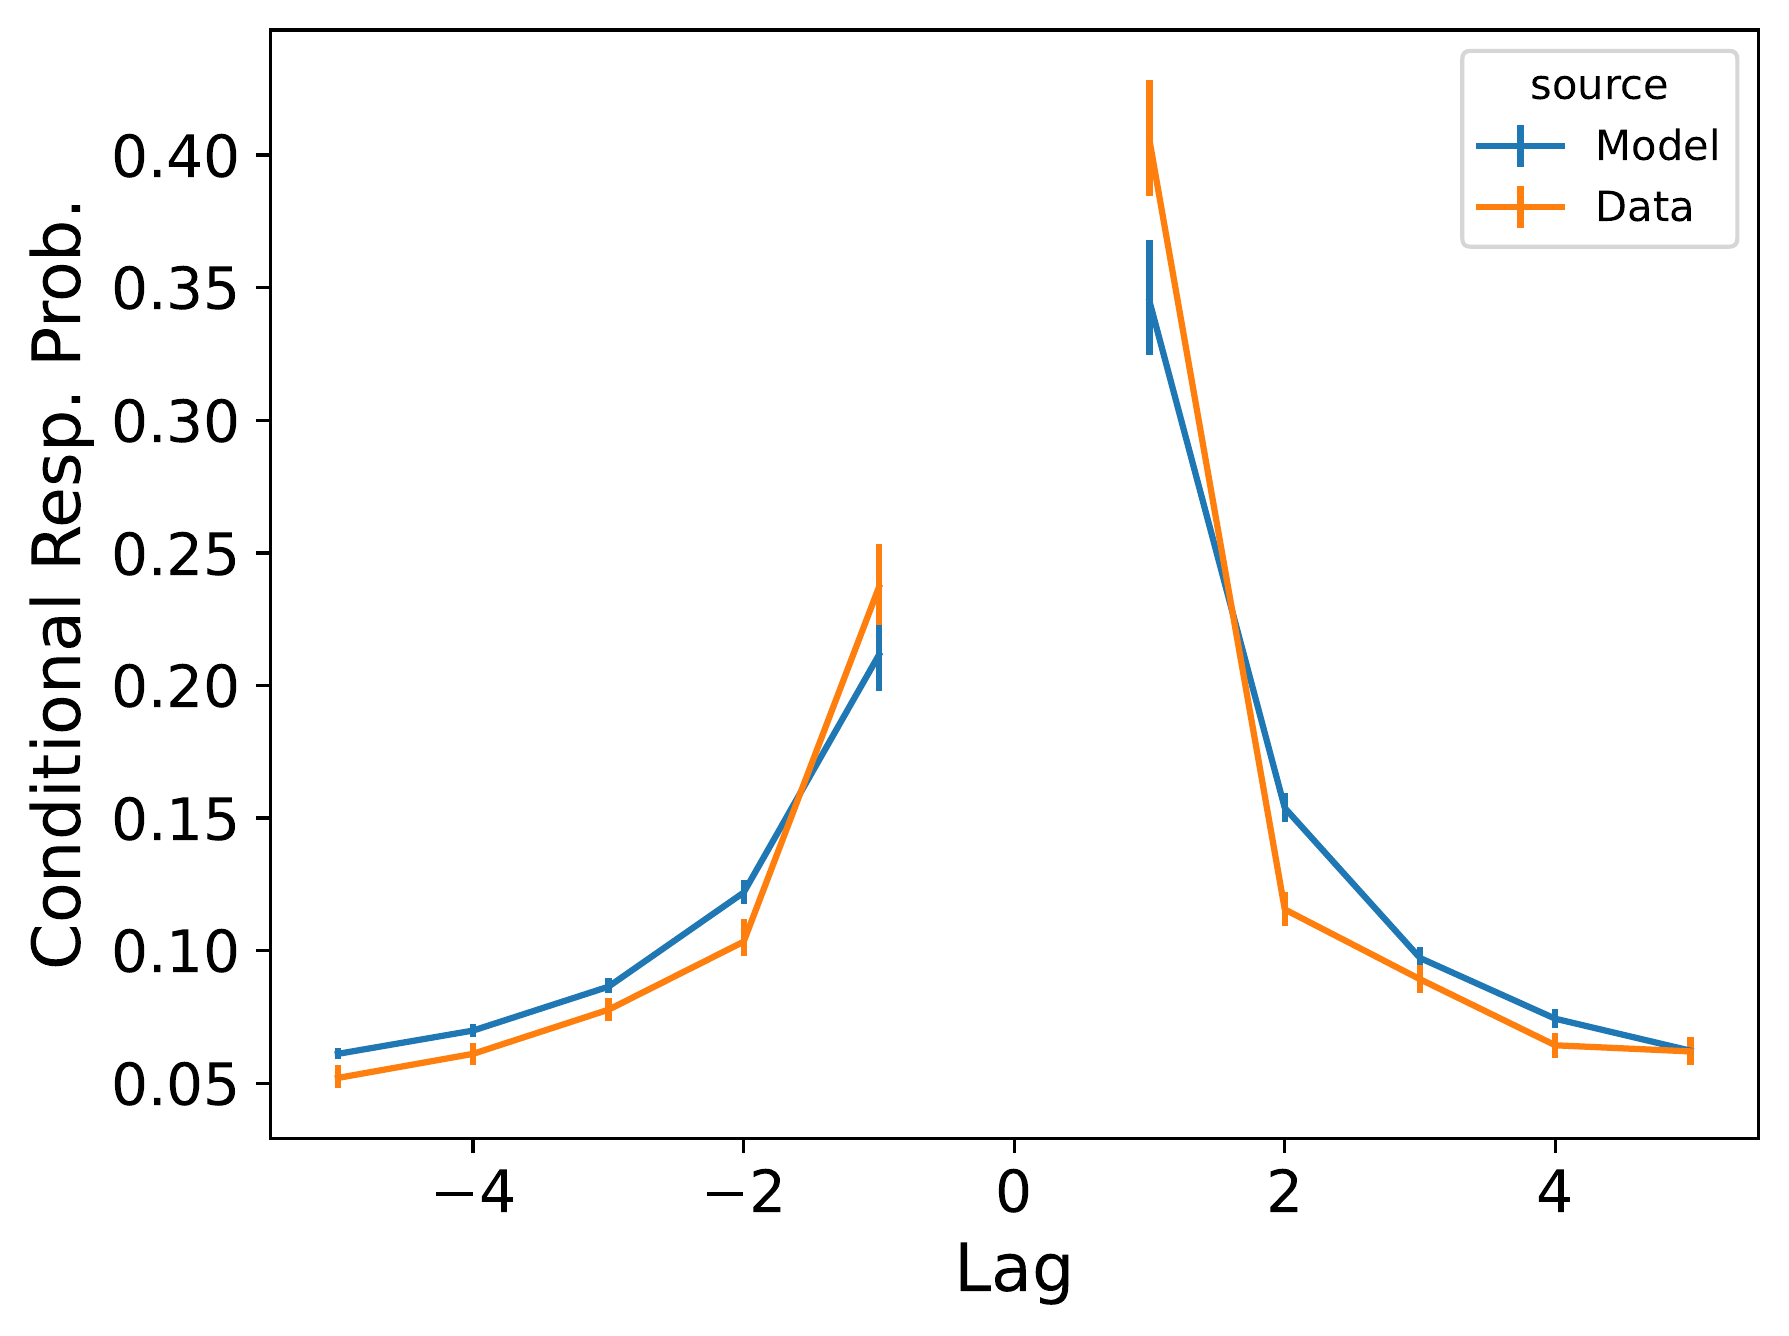
\includegraphics{icmr_figures/HealyKahana2014_ConnectionistCMR_Model_Fitting_crp-1.png}\end{minipage}%
%
\begin{minipage}{0.33\linewidth}
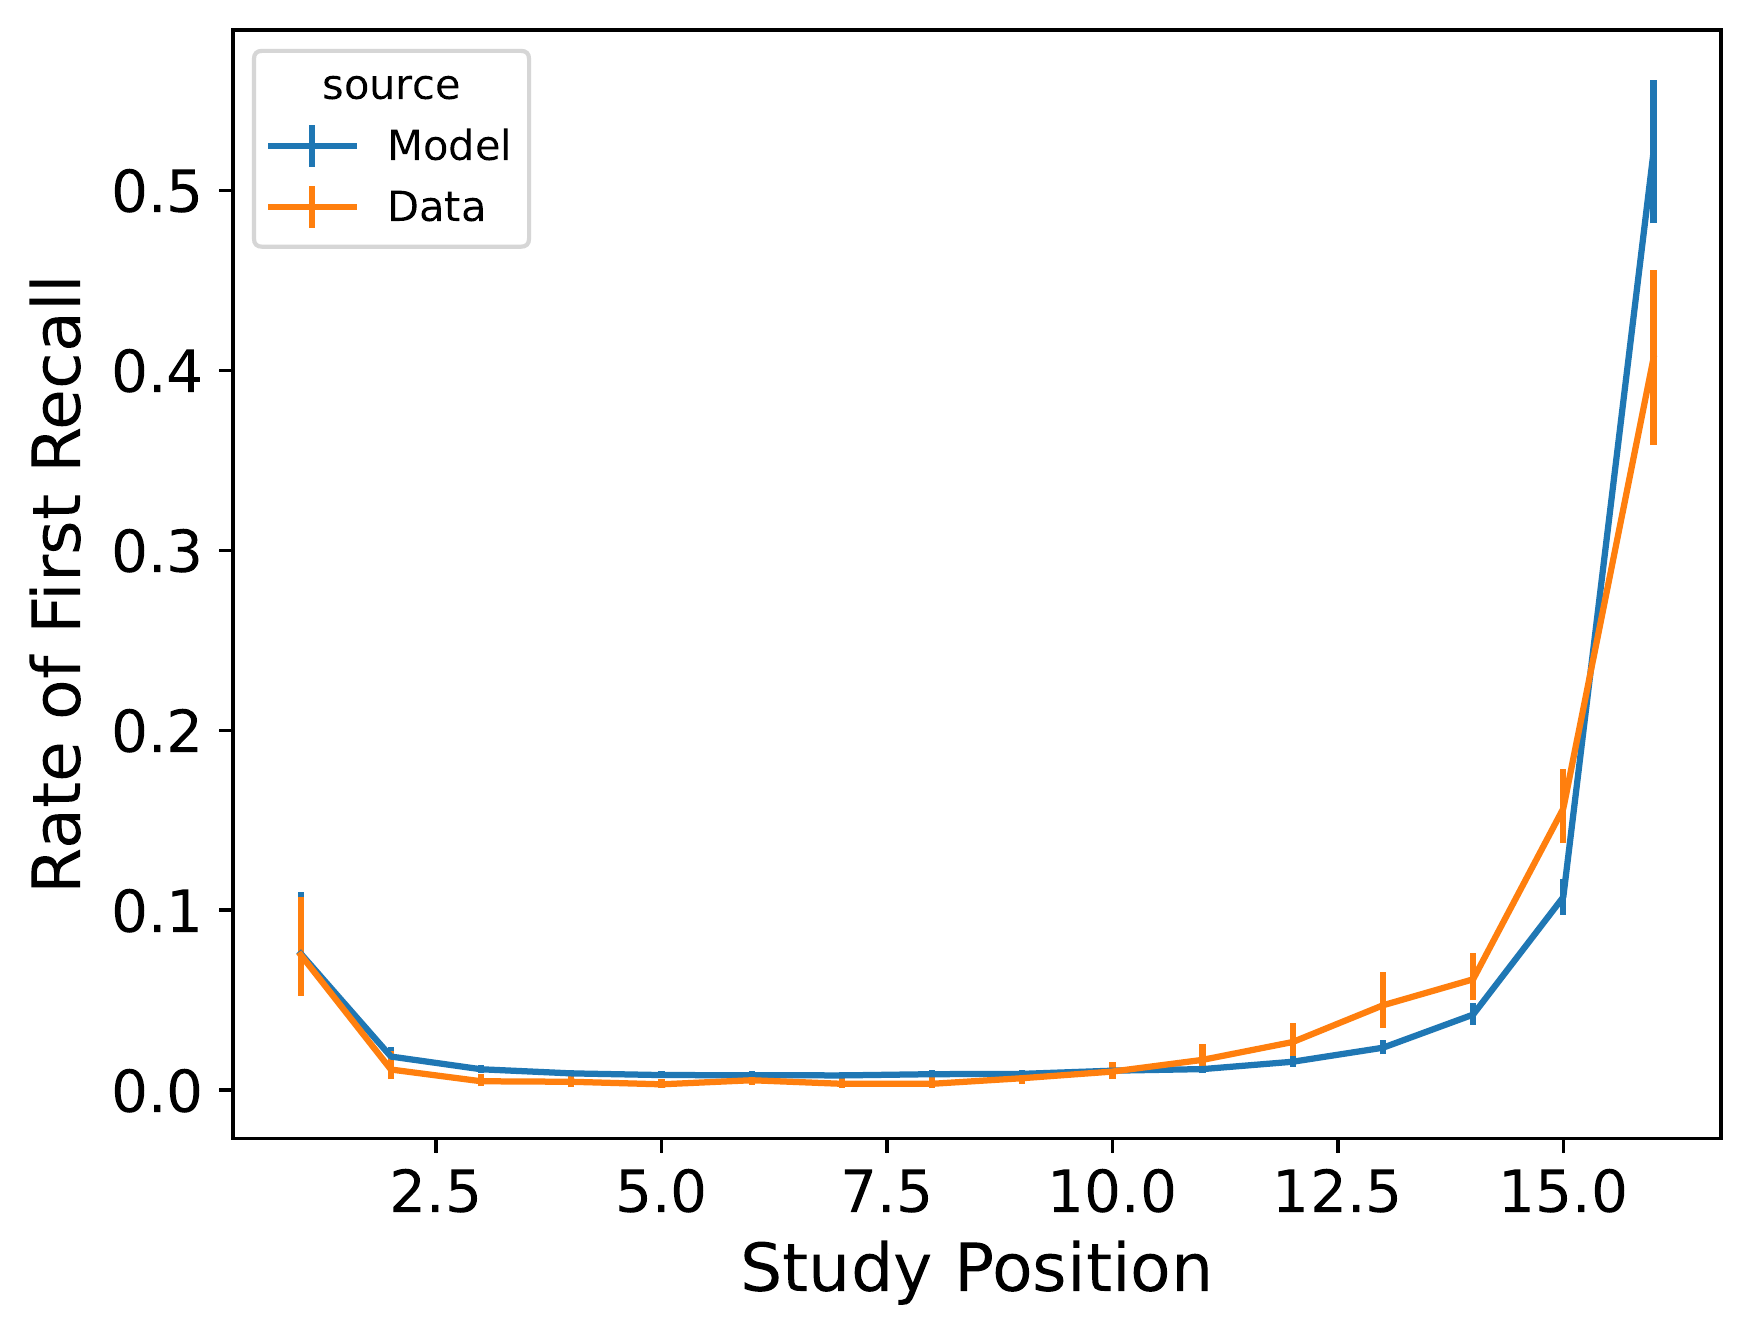
\includegraphics{icmr_figures/HealyKahana2014_ConnectionistCMR_Model_Fitting_pfr-1.png}\end{minipage}%
%
\begin{minipage}{0.33\linewidth}
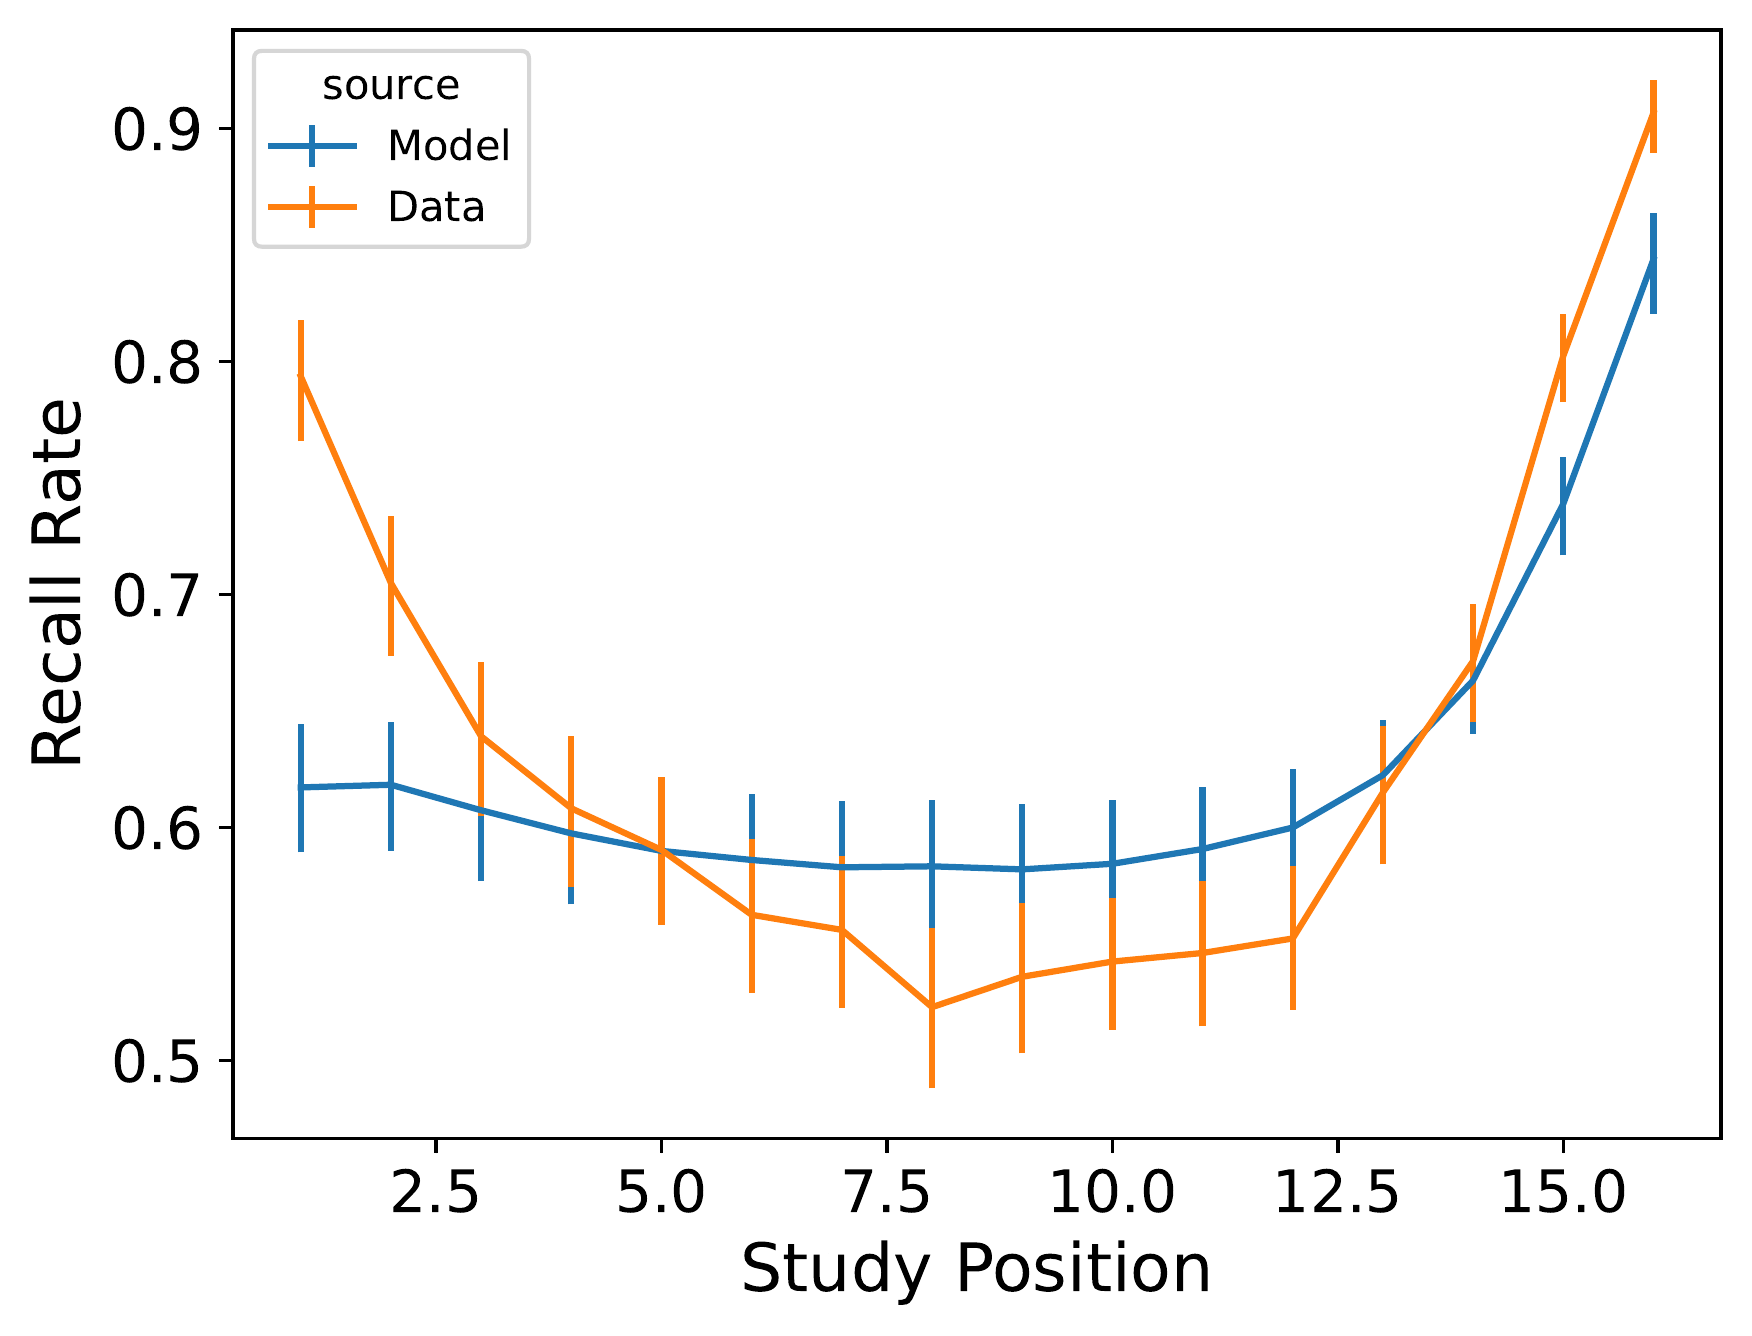
\includegraphics{icmr_figures/HealyKahana2014_ConnectionistCMR_Model_Fitting_spc-1.png}\end{minipage}%
\newline
\begin{minipage}{0.33\linewidth}
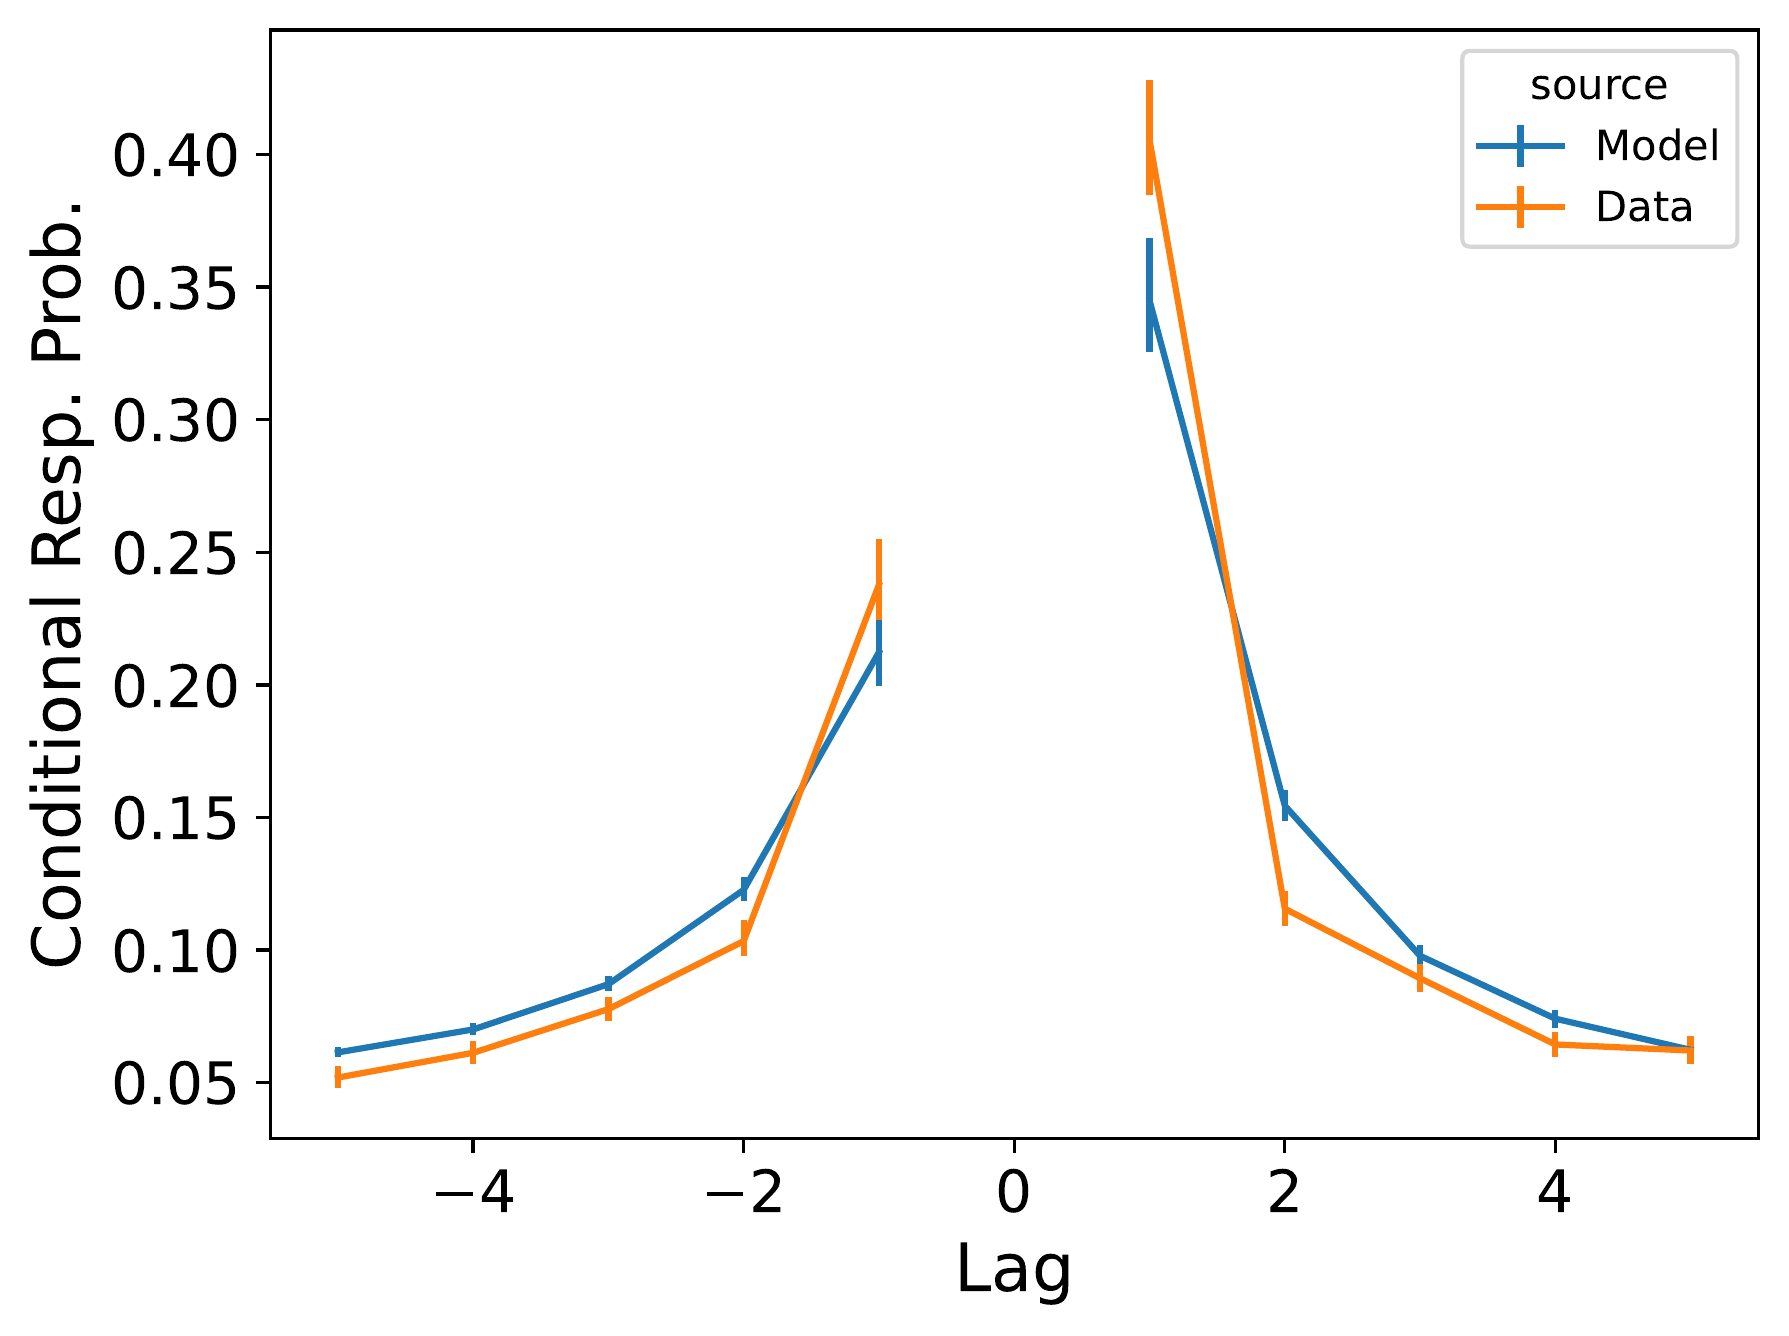
\includegraphics{icmr_figures/HealyKahana2014_InstanceCMR_Model_Fitting_crp-1.png}\end{minipage}%
%
\begin{minipage}{0.33\linewidth}
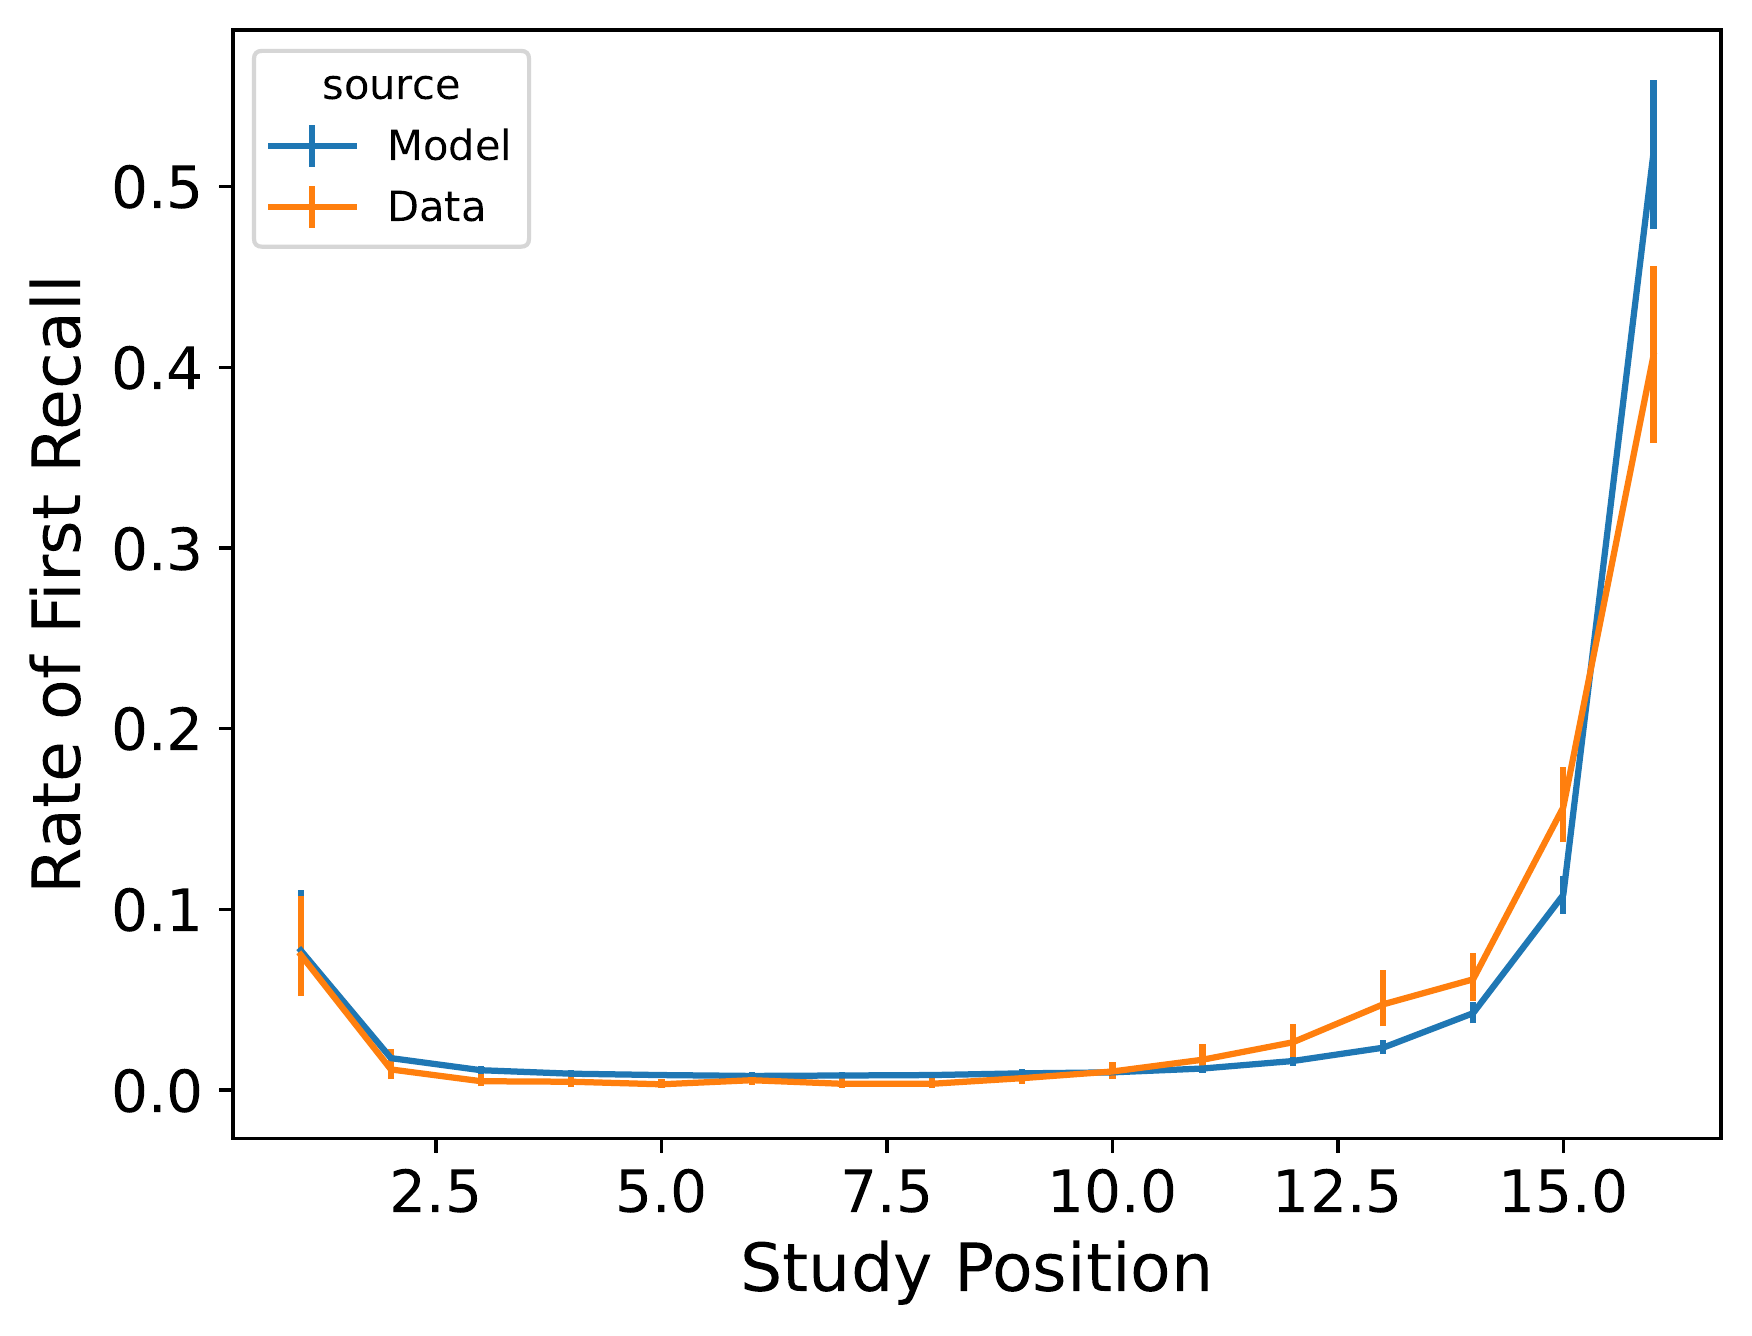
\includegraphics{icmr_figures/HealyKahana2014_InstanceCMR_Model_Fitting_pfr-1.png}\end{minipage}%
%
\begin{minipage}{0.33\linewidth}
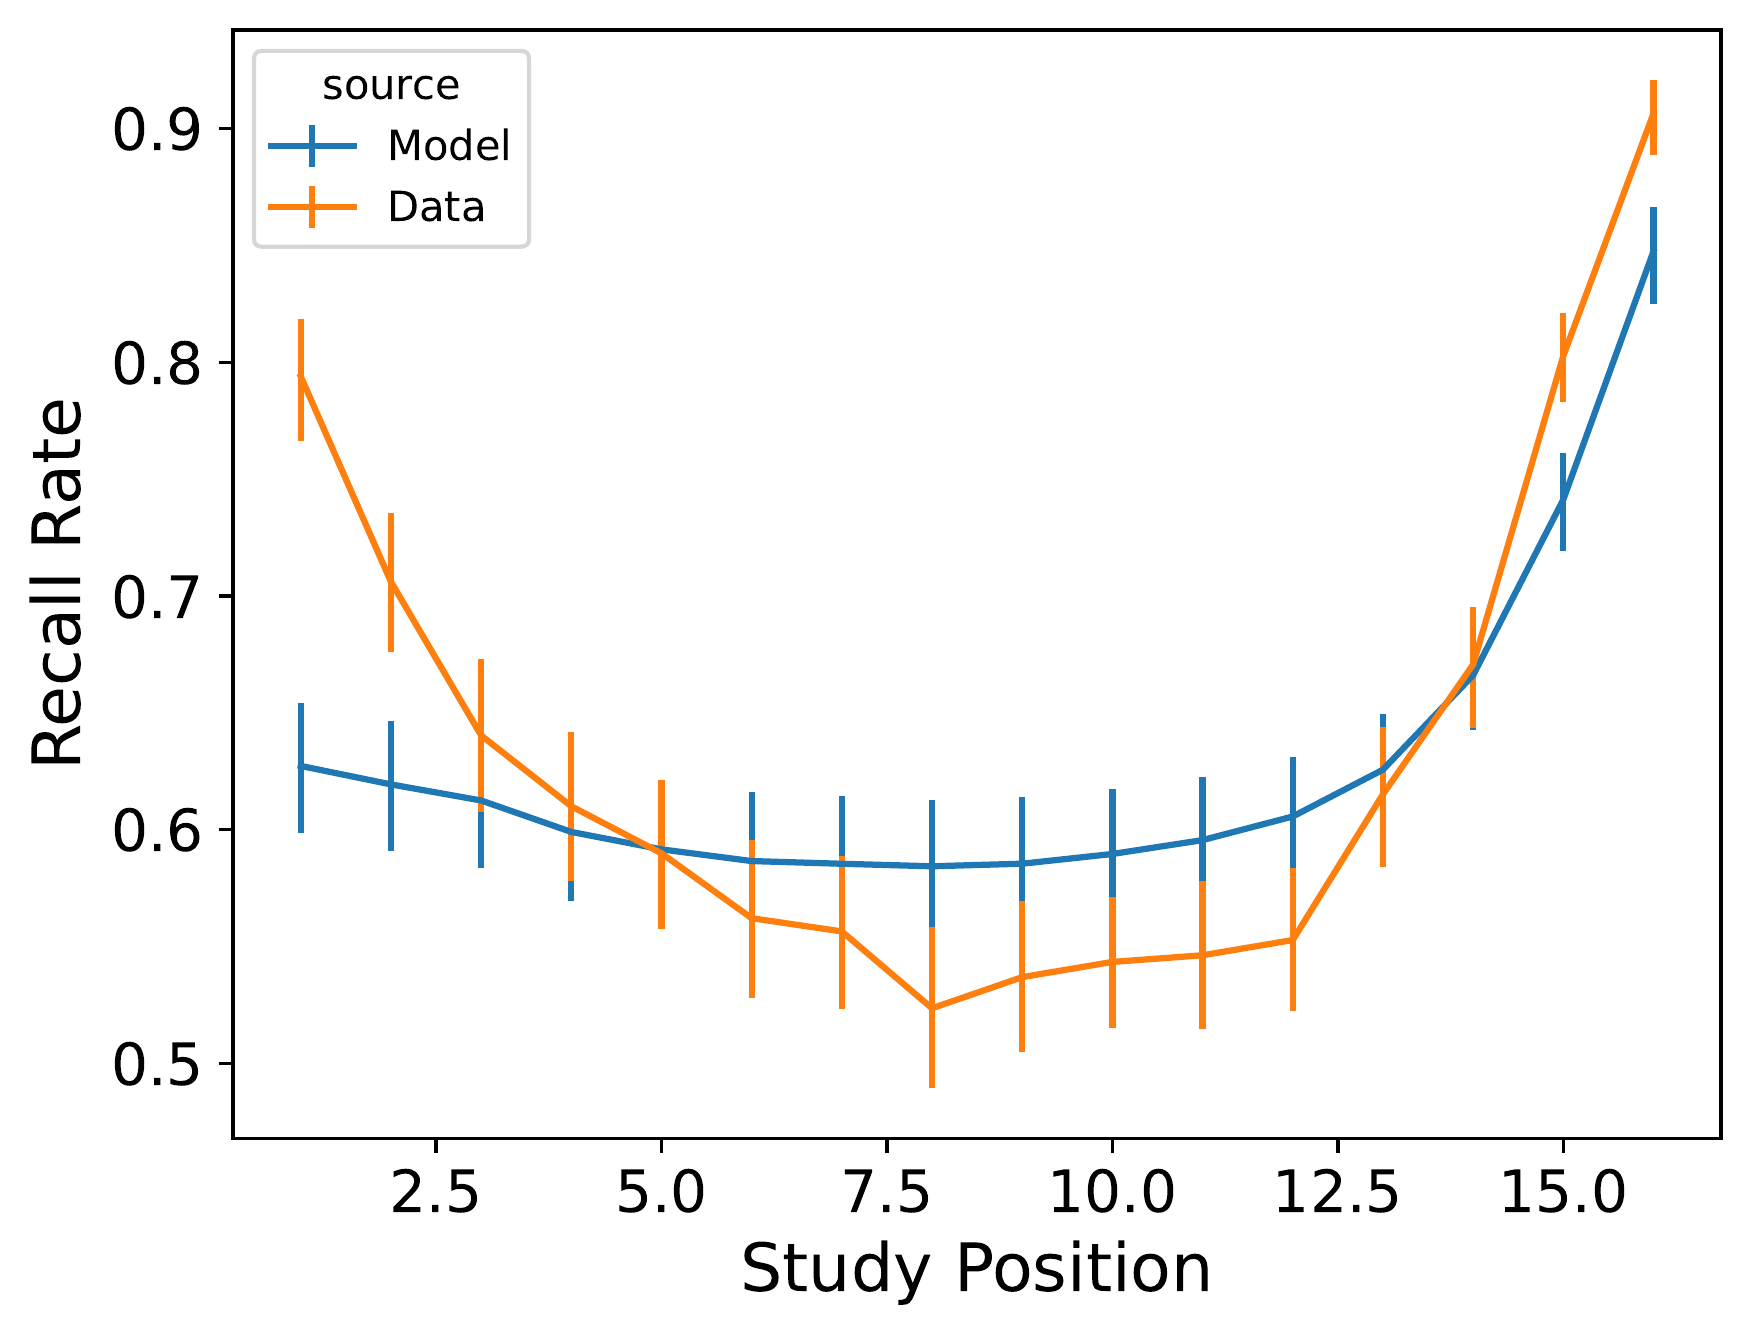
\includegraphics{icmr_figures/HealyKahana2014_InstanceCMR_Model_Fitting_spc-1.png}\end{minipage}%
\newline
\begin{minipage}{0.33\linewidth}
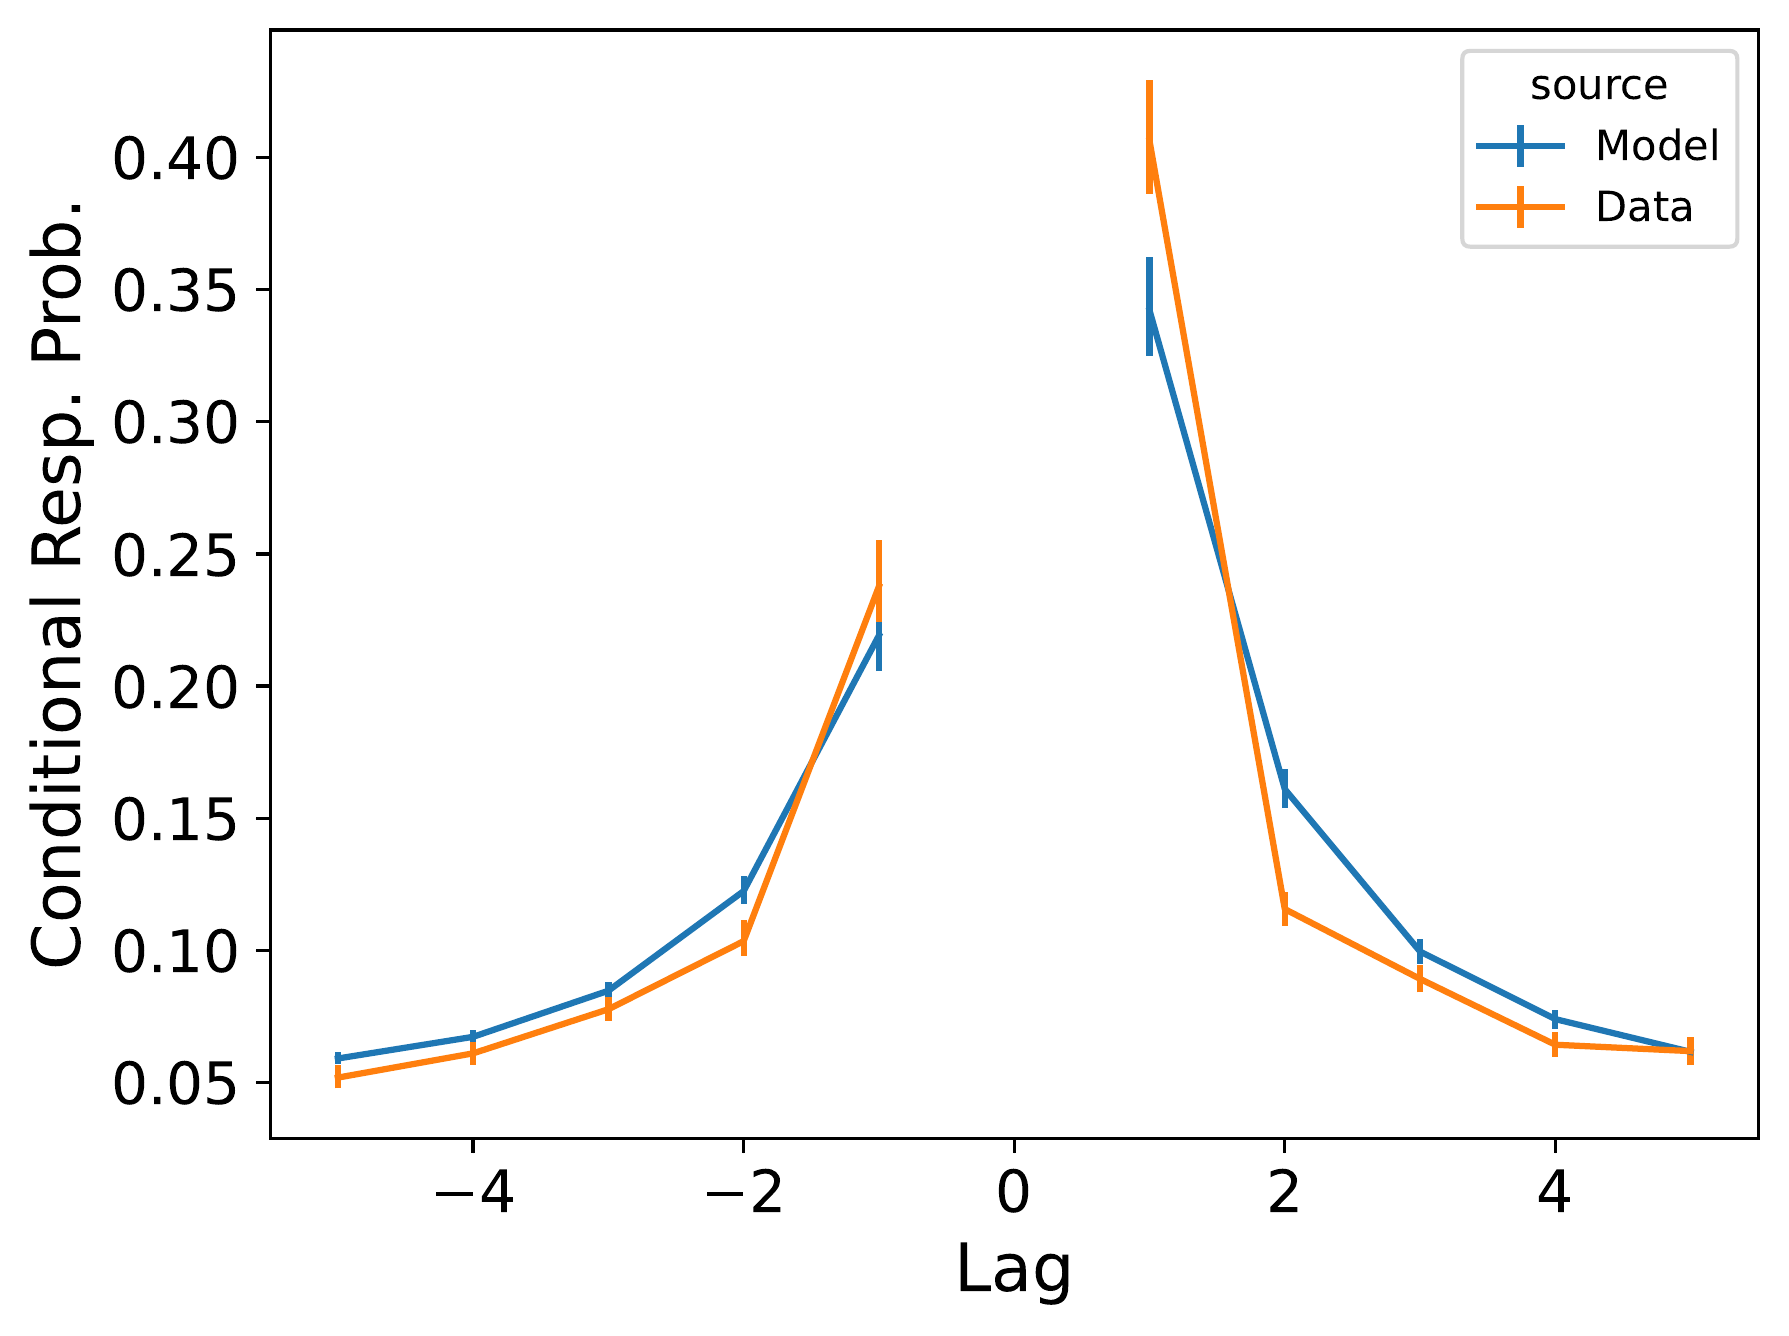
\includegraphics{icmr_figures/HealyKahana2014_TraceScalingCMR_Model_Fitting_crp-1.png}\end{minipage}%
%
\begin{minipage}{0.33\linewidth}
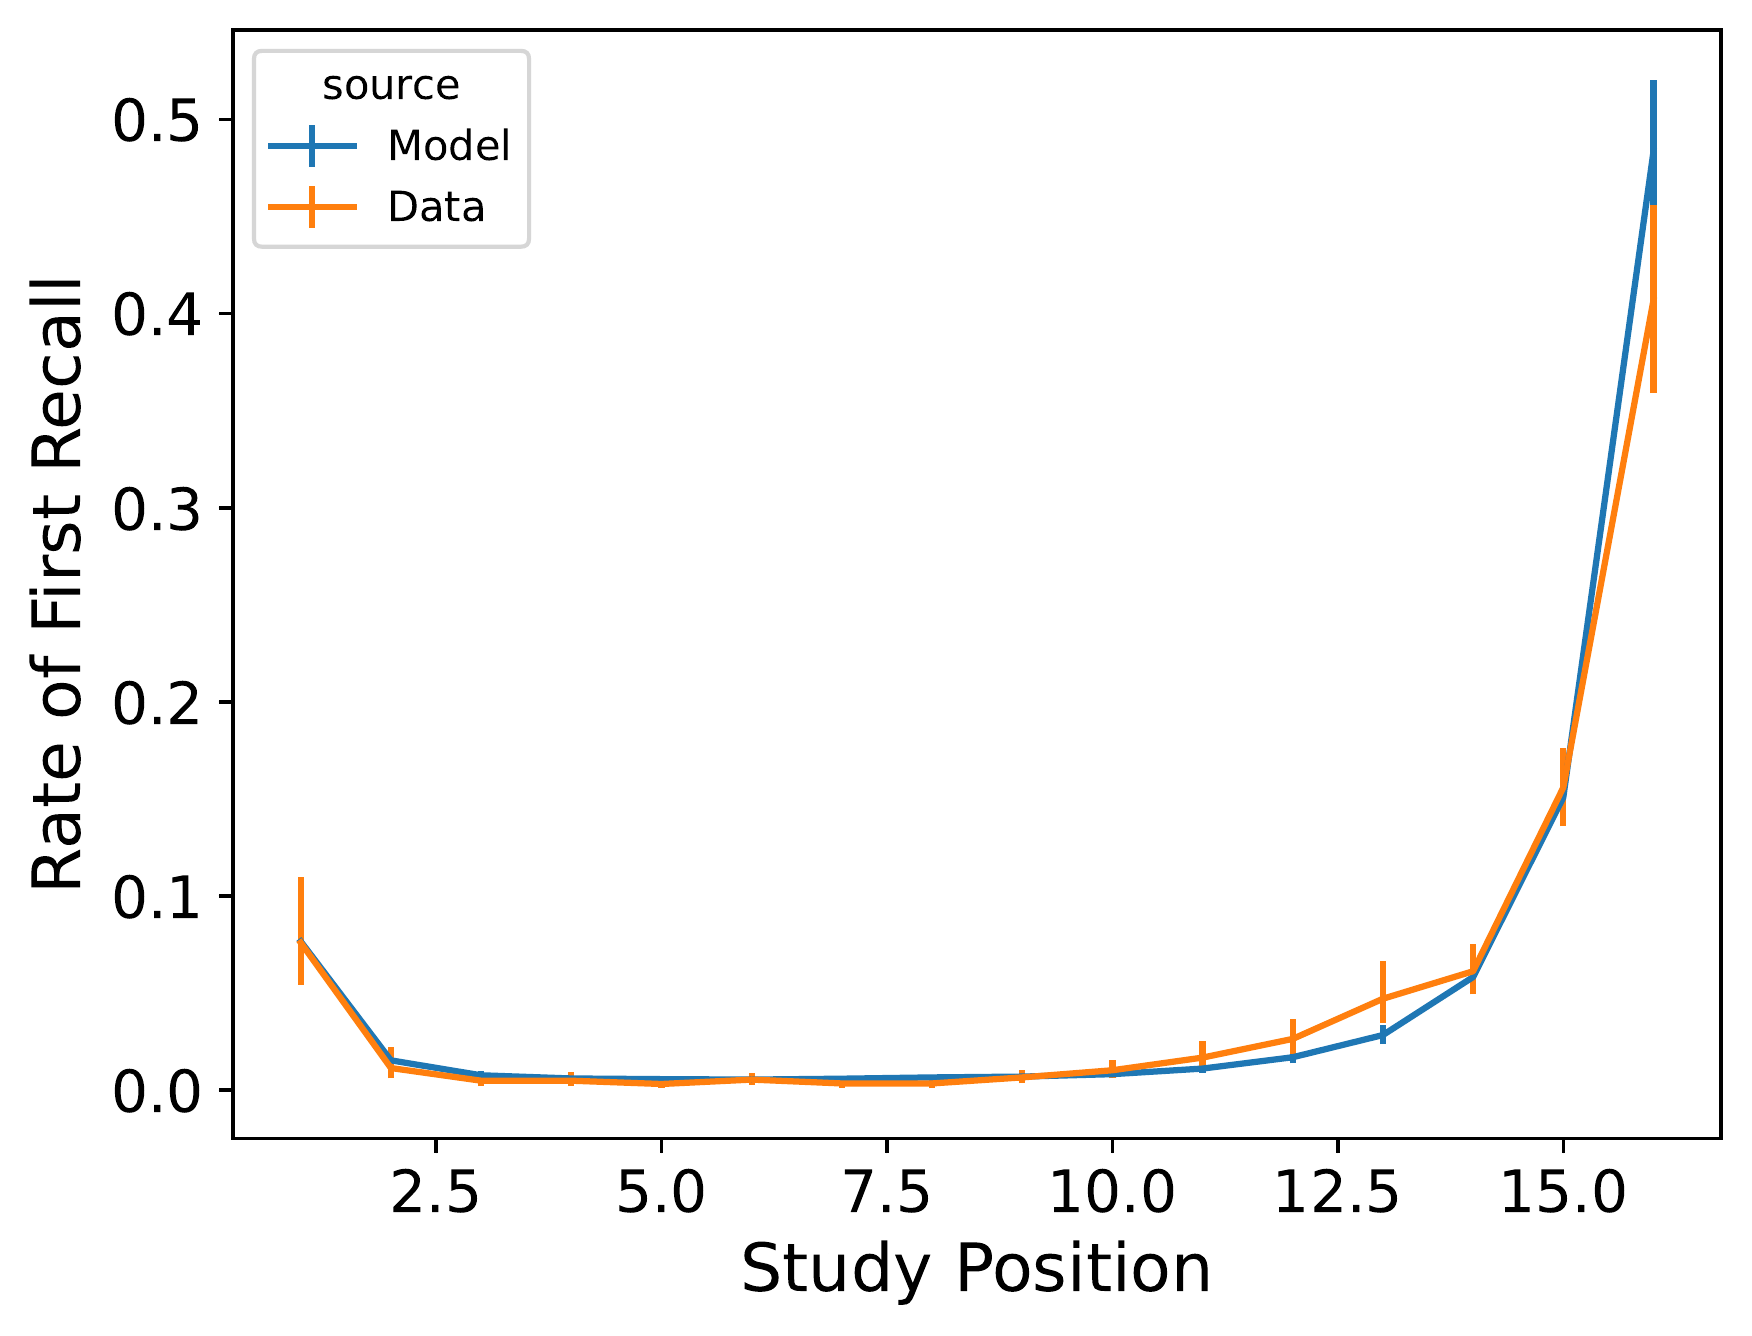
\includegraphics{icmr_figures/HealyKahana2014_TraceScalingCMR_Model_Fitting_pfr-1.png}\end{minipage}%
%
\begin{minipage}{0.33\linewidth}
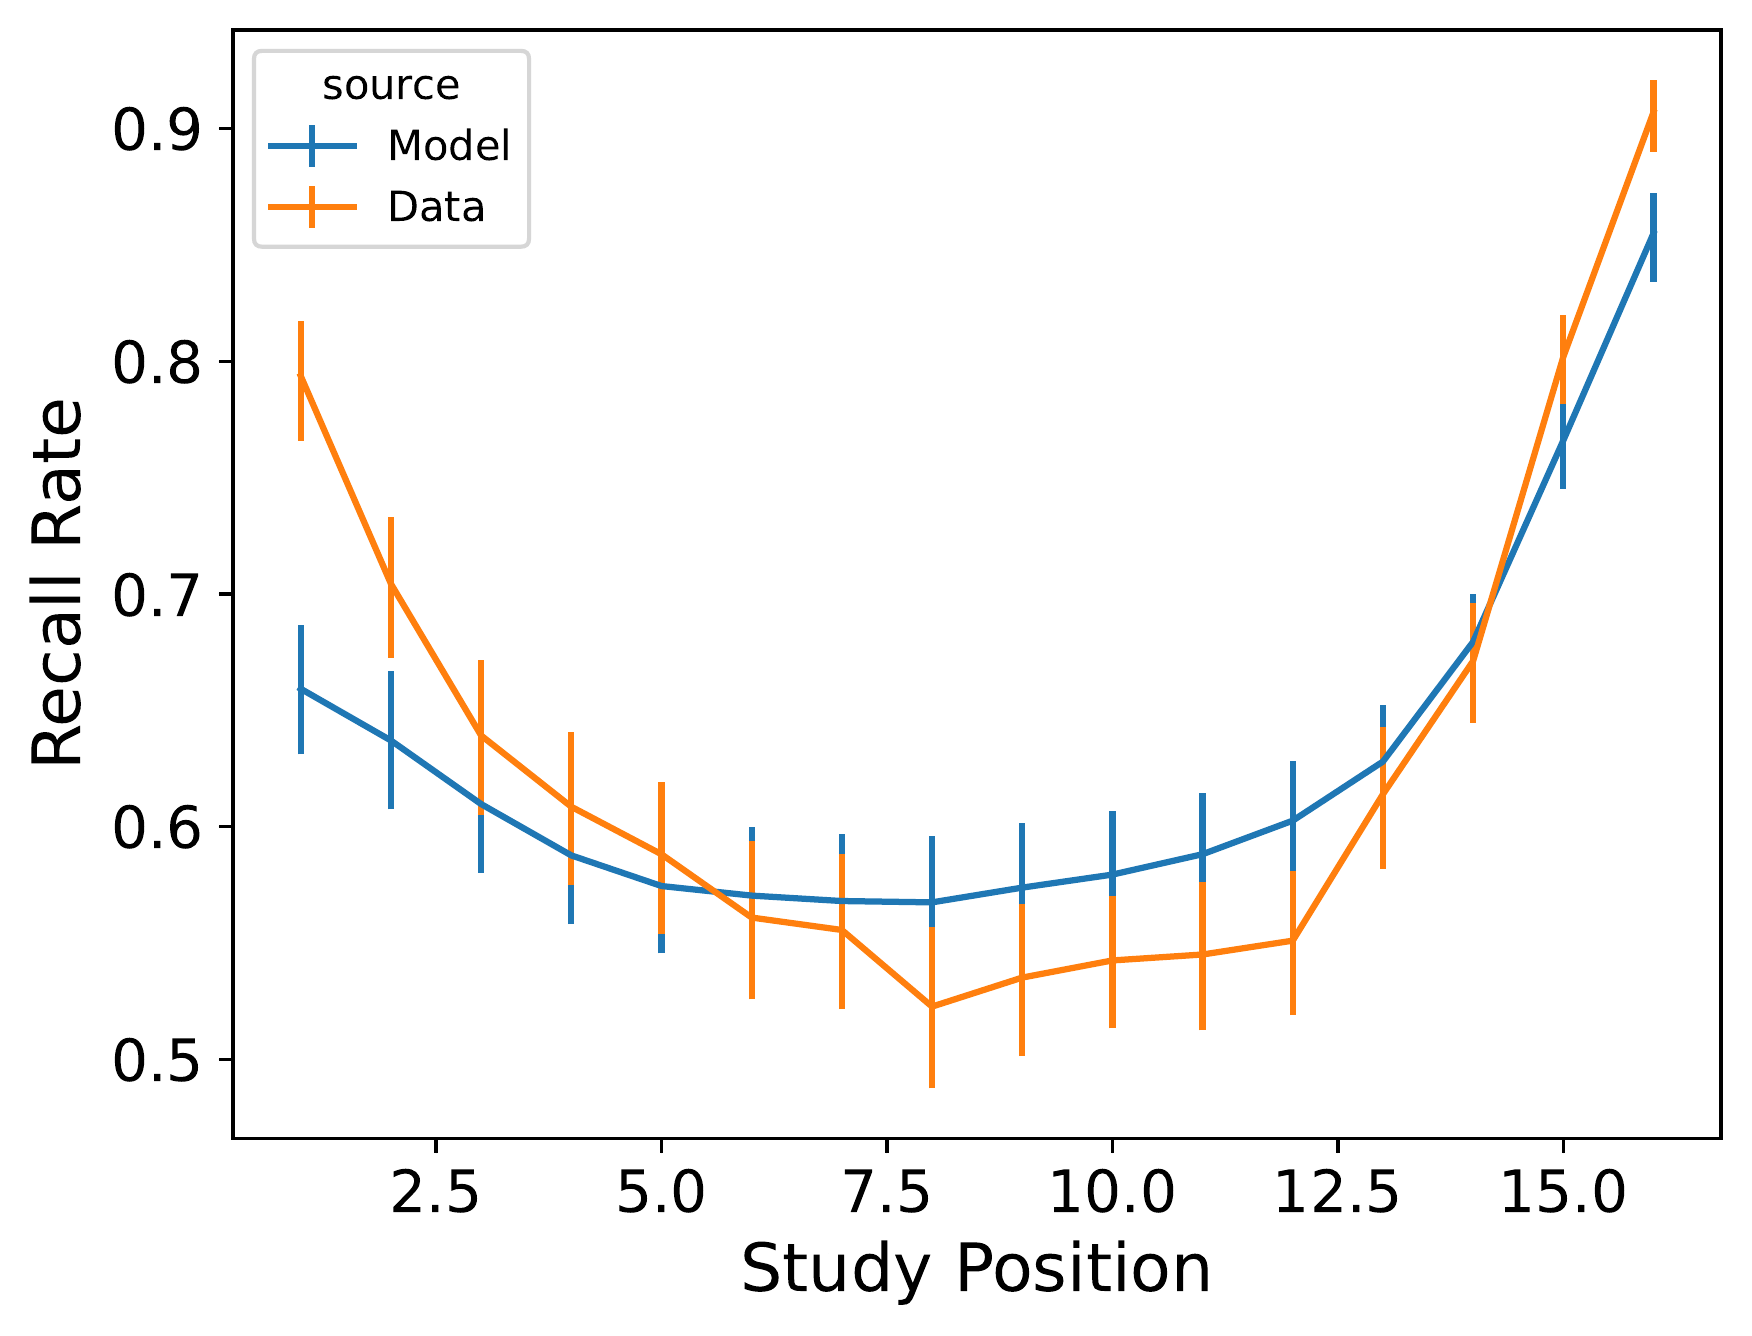
\includegraphics{icmr_figures/HealyKahana2014_TraceScalingCMR_Model_Fitting_spc-1.png}\end{minipage}%
\newline
\begin{minipage}{0.33\linewidth}
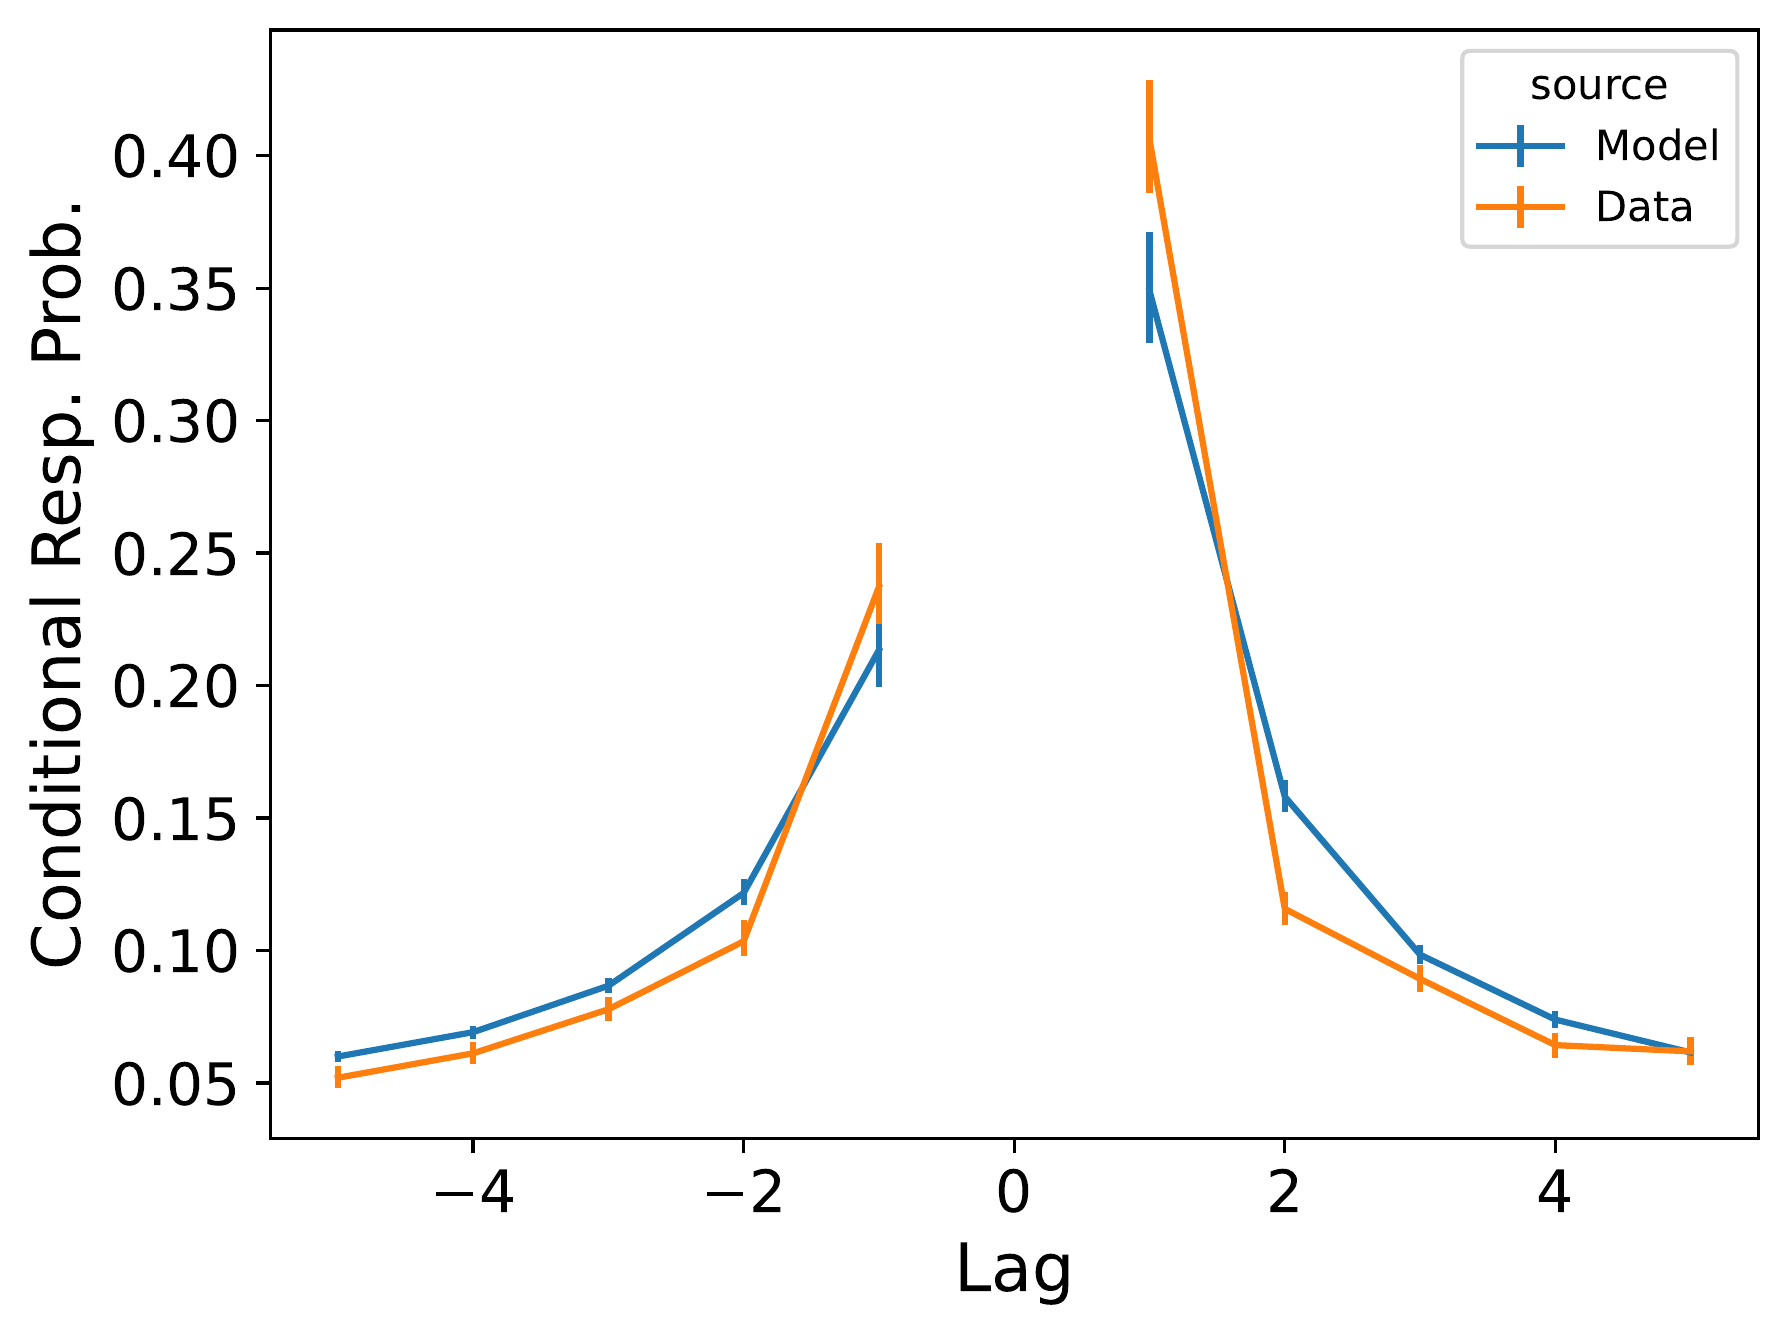
\includegraphics{icmr_figures/HealyKahana2014_MultiScalingCMR_Model_Fitting_crp-1.png}\end{minipage}%
%
\begin{minipage}{0.33\linewidth}
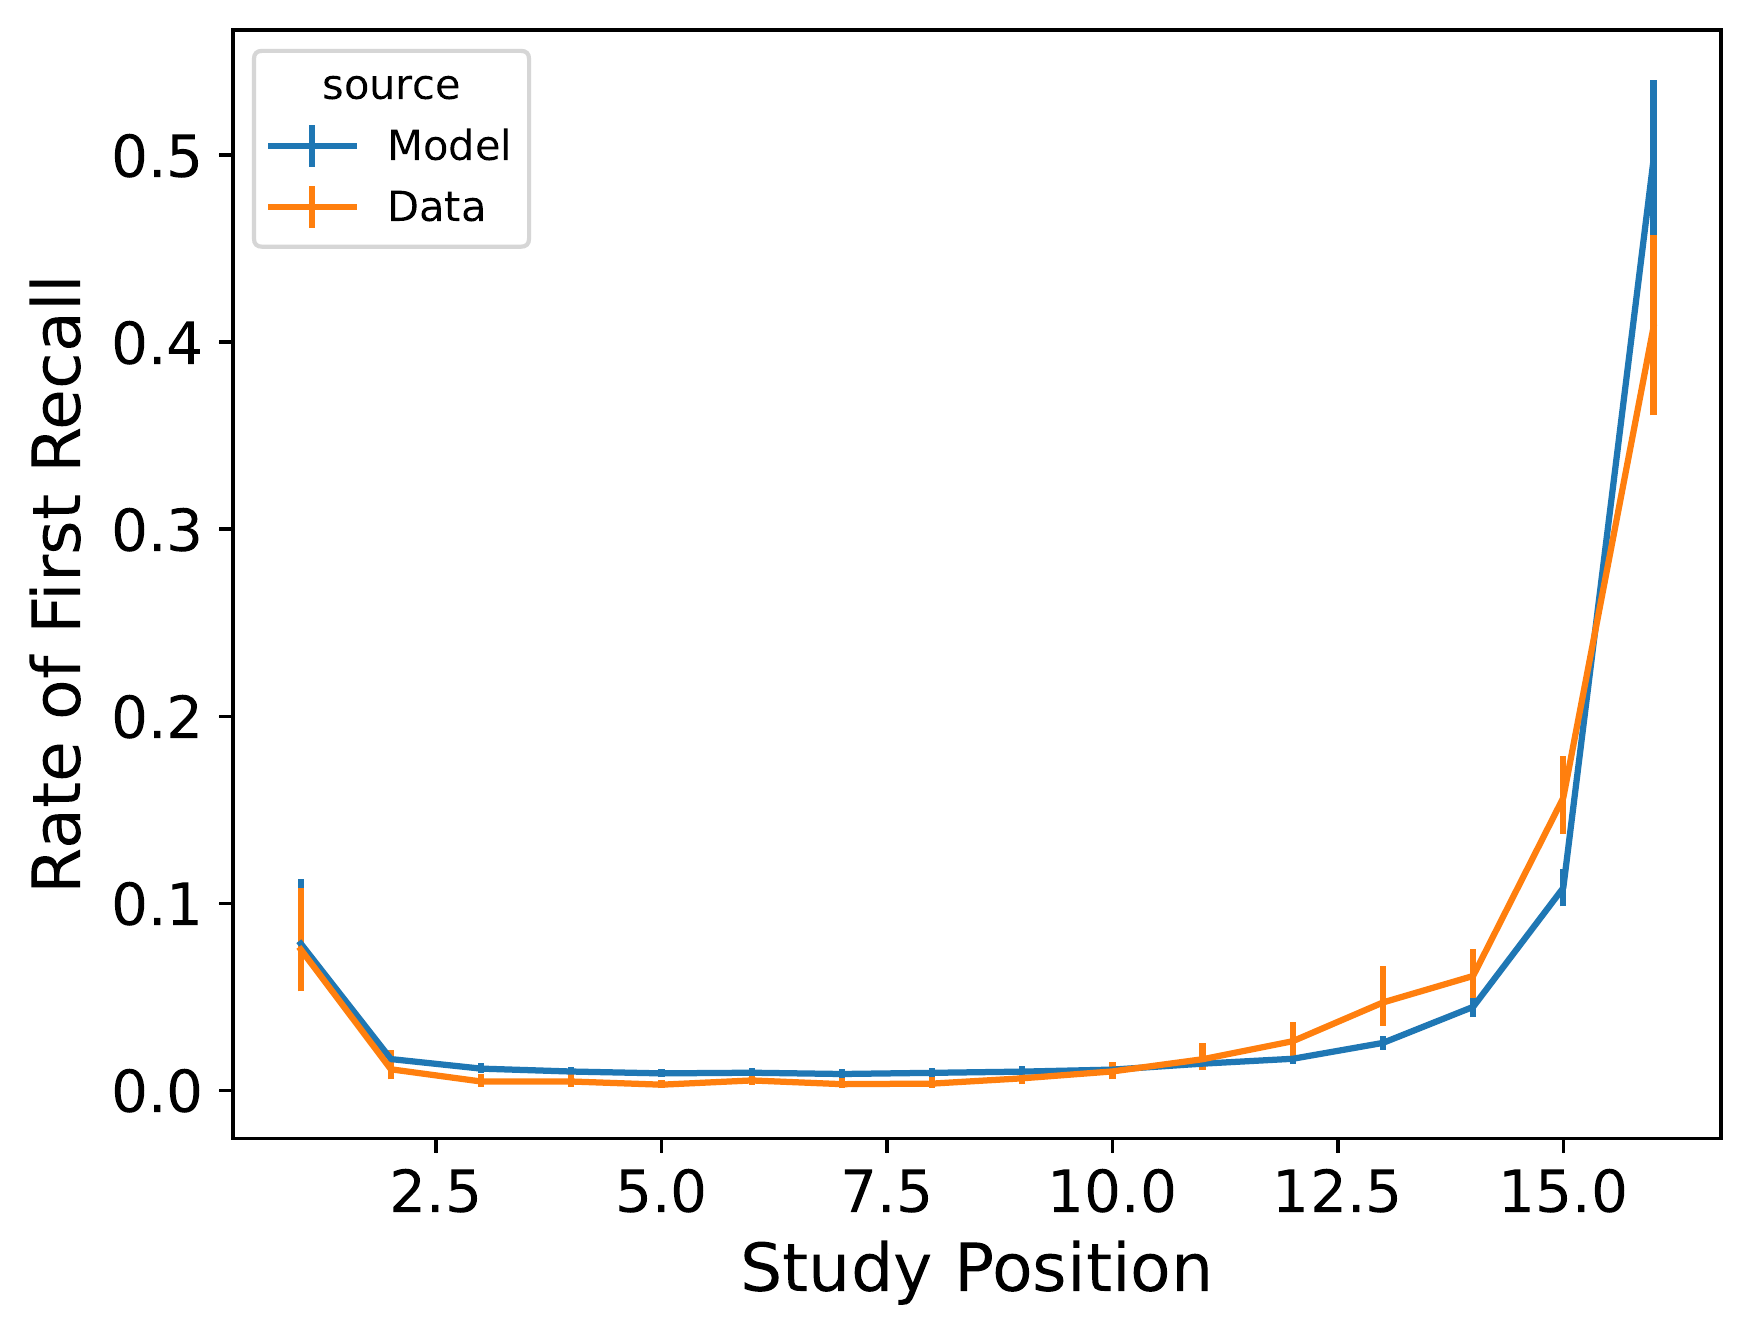
\includegraphics{icmr_figures/HealyKahana2014_MultiScalingCMR_Model_Fitting_pfr-1.png}\end{minipage}%
%
\begin{minipage}{0.33\linewidth}
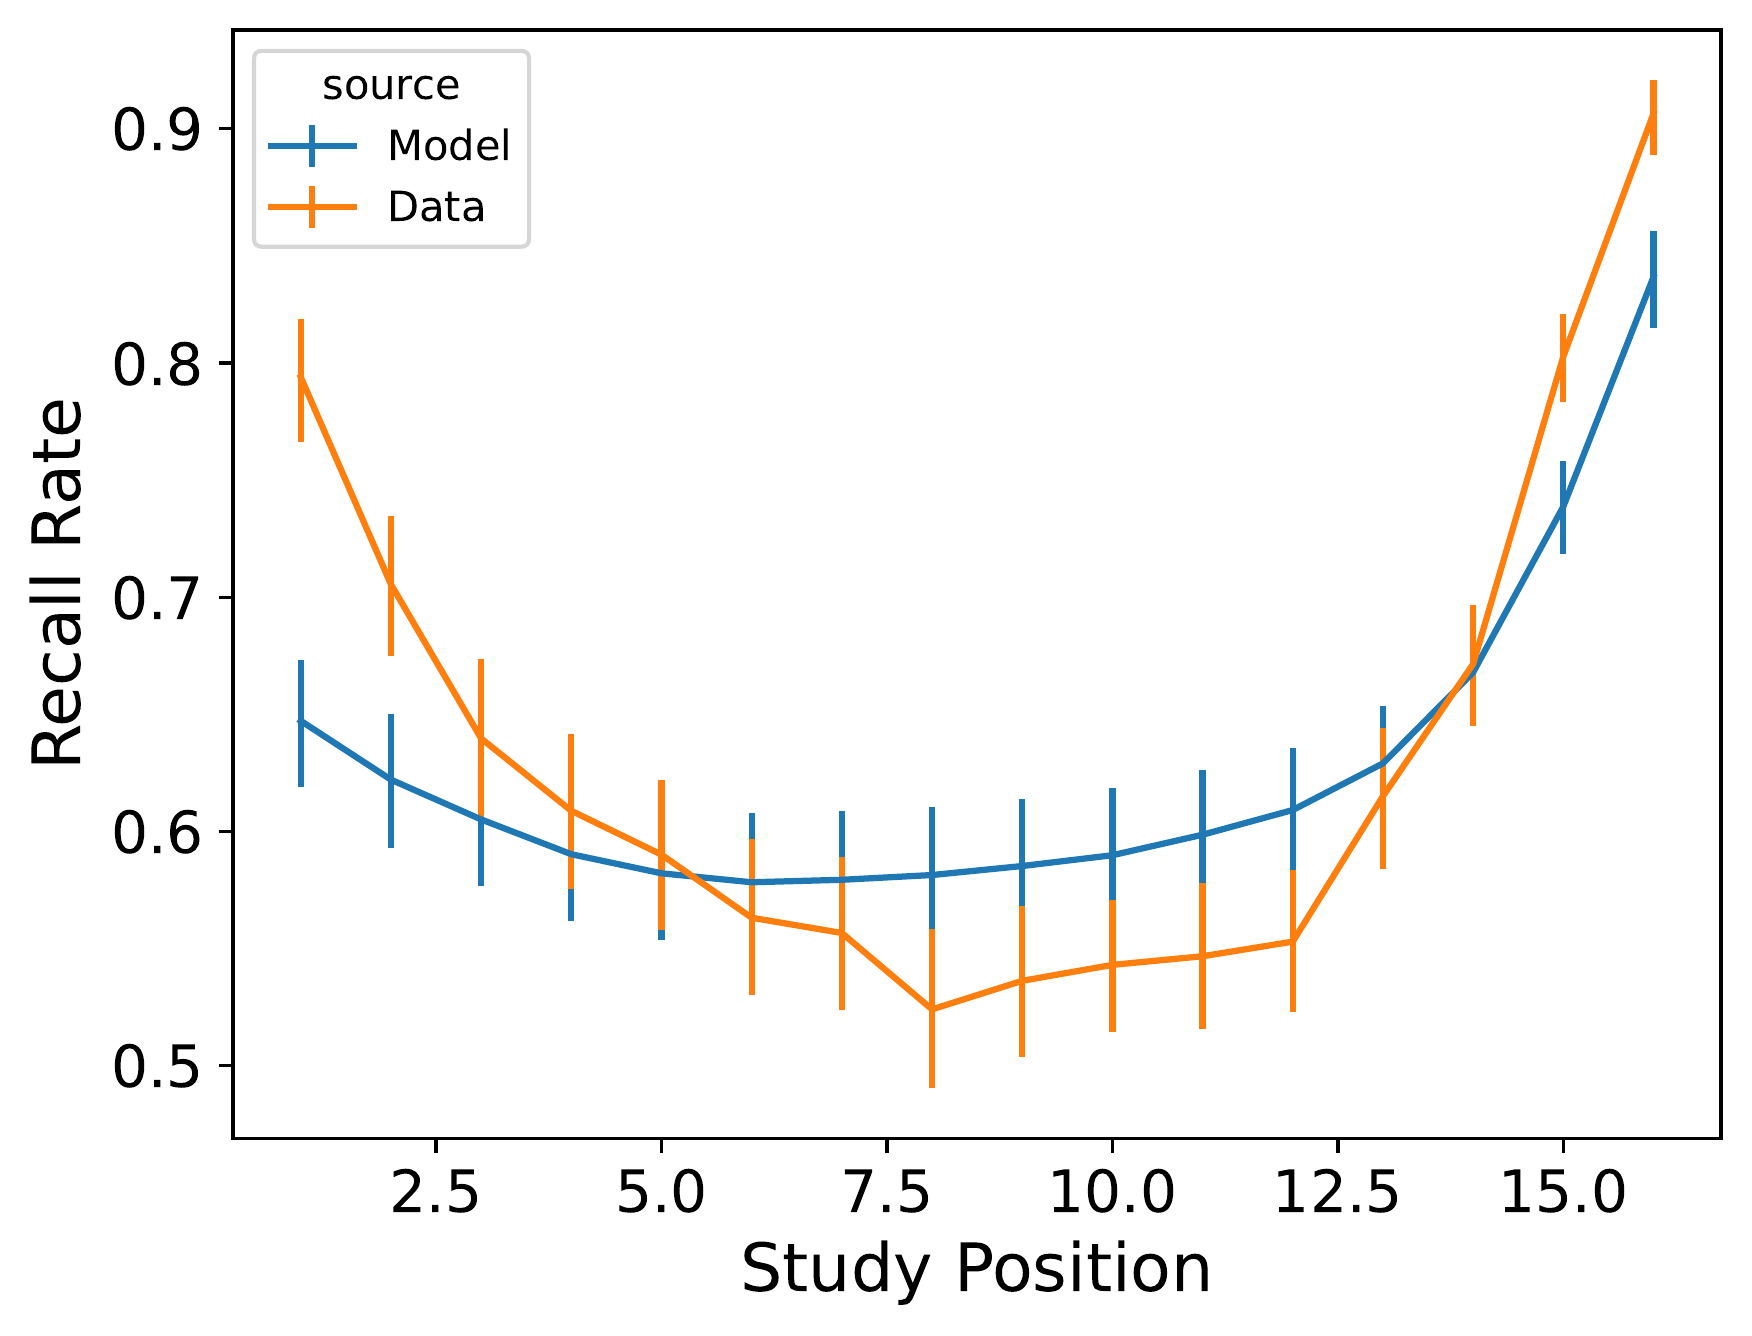
\includegraphics{icmr_figures/HealyKahana2014_MultiScalingCMR_Model_Fitting_spc-1.png}\end{minipage}%

\caption{\label{fig-healey2014memory}Summary statistic fits to Healey
and Kahana (2014). Top: Connectionist CMR. Second Row: Instance CMR,
\(\tau_{t}\) set to 1. Third Row: Trace Scaling CMR -- Instance CMR,
\(\tau_{c}\) set to 1 and \(\tau_{t}\) optimized during fitting. Fourth
Row: Multi Scaling CMR -- Instance CMR, both \(\tau_{t}\) and
\(\tau_{c}\) optimized during fitting. Left: conditional response
probability as a function of lag. Middle: probability of starting recall
by serial position. Right: recall probability by serial position.}

\end{figure}%

\newpage{}

\subsubsection{Murdock (1962)}\label{murdock-1962}

\begin{longtable}[]{@{}
  >{\raggedright\arraybackslash}p{(\columnwidth - 10\tabcolsep) * \real{0.2800}}
  >{\raggedright\arraybackslash}p{(\columnwidth - 10\tabcolsep) * \real{0.1400}}
  >{\raggedright\arraybackslash}p{(\columnwidth - 10\tabcolsep) * \real{0.1400}}
  >{\raggedright\arraybackslash}p{(\columnwidth - 10\tabcolsep) * \real{0.1400}}
  >{\raggedright\arraybackslash}p{(\columnwidth - 10\tabcolsep) * \real{0.1400}}
  >{\raggedright\arraybackslash}p{(\columnwidth - 10\tabcolsep) * \real{0.1400}}@{}}
\caption{Confidence intervals of parameters fit to data from Murdock Jr
(1962), computed across subjects. Column 1: Connectionist CMR follows
the specification in Morton and Polyn (2016). Column 2: Instance CMR
with trace activation scaling turned off. Column 3: Instance CMR with
only trace activation scaling and no item activation scaling. Fourth
model Column 4: Instance CMR with both trace and item activation scaling
parameters freed for fitting. }\label{tbl-murdock}\tabularnewline
\toprule\noalign{}
\begin{minipage}[b]{\linewidth}\raggedright
\end{minipage} & \begin{minipage}[b]{\linewidth}\raggedright
Connectionist CMR
\end{minipage} & \begin{minipage}[b]{\linewidth}\raggedright
Instance CMR
\end{minipage} & \begin{minipage}[b]{\linewidth}\raggedright
Trace Scaling CMR
\end{minipage} & \begin{minipage}[b]{\linewidth}\raggedright
Multi Scaling CMR
\end{minipage} & \begin{minipage}[b]{\linewidth}\raggedright
\end{minipage} \\
\midrule\noalign{}
\endfirsthead
\toprule\noalign{}
\begin{minipage}[b]{\linewidth}\raggedright
\end{minipage} & \begin{minipage}[b]{\linewidth}\raggedright
Connectionist CMR
\end{minipage} & \begin{minipage}[b]{\linewidth}\raggedright
Instance CMR
\end{minipage} & \begin{minipage}[b]{\linewidth}\raggedright
Trace Scaling CMR
\end{minipage} & \begin{minipage}[b]{\linewidth}\raggedright
Multi Scaling CMR
\end{minipage} & \begin{minipage}[b]{\linewidth}\raggedright
\end{minipage} \\
\midrule\noalign{}
\endhead
\bottomrule\noalign{}
\endlastfoot
fitness & 5260.73 +/- 290.76 & 5283.63 +/- 303.93 & 5287.44 +/- 302.87 &
5267.38 +/- 304.15 & \\
encoding drift rate & 0.47 +/- 0.09 & 0.51 +/- 0.09 & 0.58 +/- 0.13 &
0.61 +/- 0.13 & \\
start drift rate & 0.21 +/- 0.13 & 0.20 +/- 0.13 & 0.12 +/- 0.07 & 0.27
+/- 0.19 & \\
recall drift rate & 0.87 +/- 0.05 & 0.84 +/- 0.06 & 0.90 +/- 0.02 & 0.93
+/- 0.03 & \\
shared support & 3.37 +/- 4.11 & 6.00 +/- 7.87 & 0.03 +/- 0.01 & 7.12
+/- 5.62 & \\
item support & 17.00 +/- 13.71 & 27.35 +/- 20.16 & 45.09 +/- 16.45 &
25.82 +/- 21.40 & \\
learning rate & 0.14 +/- 0.07 & 0.11 +/- 0.05 & 0.17 +/- 0.09 & 0.13 +/-
0.13 & \\
primacy scale & 15.93 +/- 14.21 & 21.36 +/- 17.07 & 54.97 +/- 13.58 &
10.24 +/- 8.70 & \\
primacy decay & 25.26 +/- 21.17 & 14.94 +/- 14.91 & 26.49 +/- 19.13 &
19.80 +/- 17.12 & \\
stop probability scale & 0.02 +/- 0.00 & 0.02 +/- 0.00 & 0.02 +/- 0.00 &
0.02 +/- 0.00 & \\
stop probability growth & 0.28 +/- 0.02 & 0.29 +/- 0.02 & 0.28 +/- 0.02
& 0.28 +/- 0.02 & \\
choice sensitivity & 30.78 +/- 19.05 & 38.38 +/- 22.18 & 1.00 +/- 0.00 &
37.44 +/- 17.25 & \\
mcf trace sensitivity & 1.00 +/- 0.00 & 1.00 +/- 0.00 & 3.24 +/- 1.13 &
1.13 +/- 0.84 & \\
\end{longtable}

\begin{figure}

\begin{minipage}{0.33\linewidth}
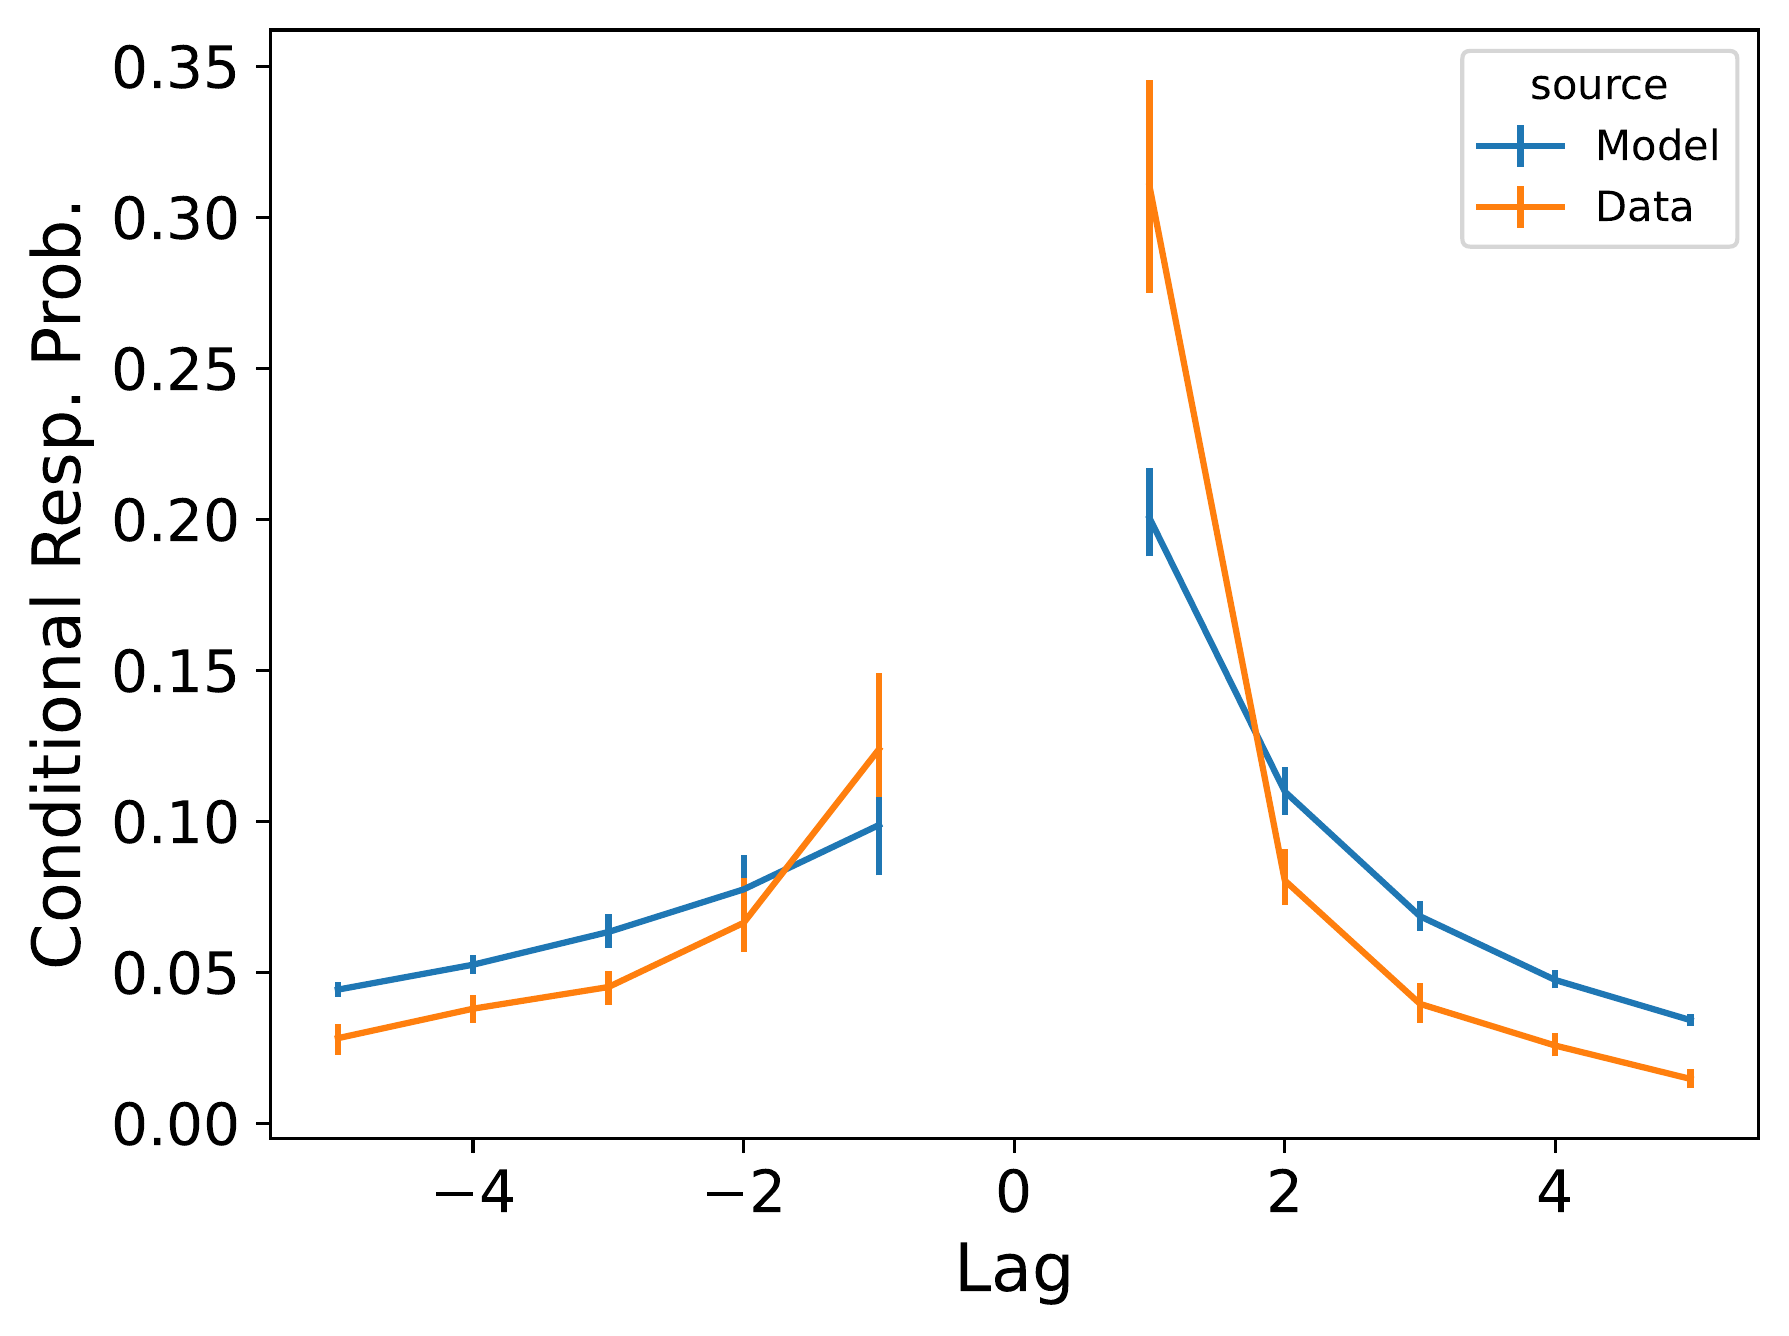
\includegraphics{icmr_figures/Murdock1962_ConnectionistCMR_Model_Fitting_LL20_crp-1.png}\end{minipage}%
%
\begin{minipage}{0.33\linewidth}
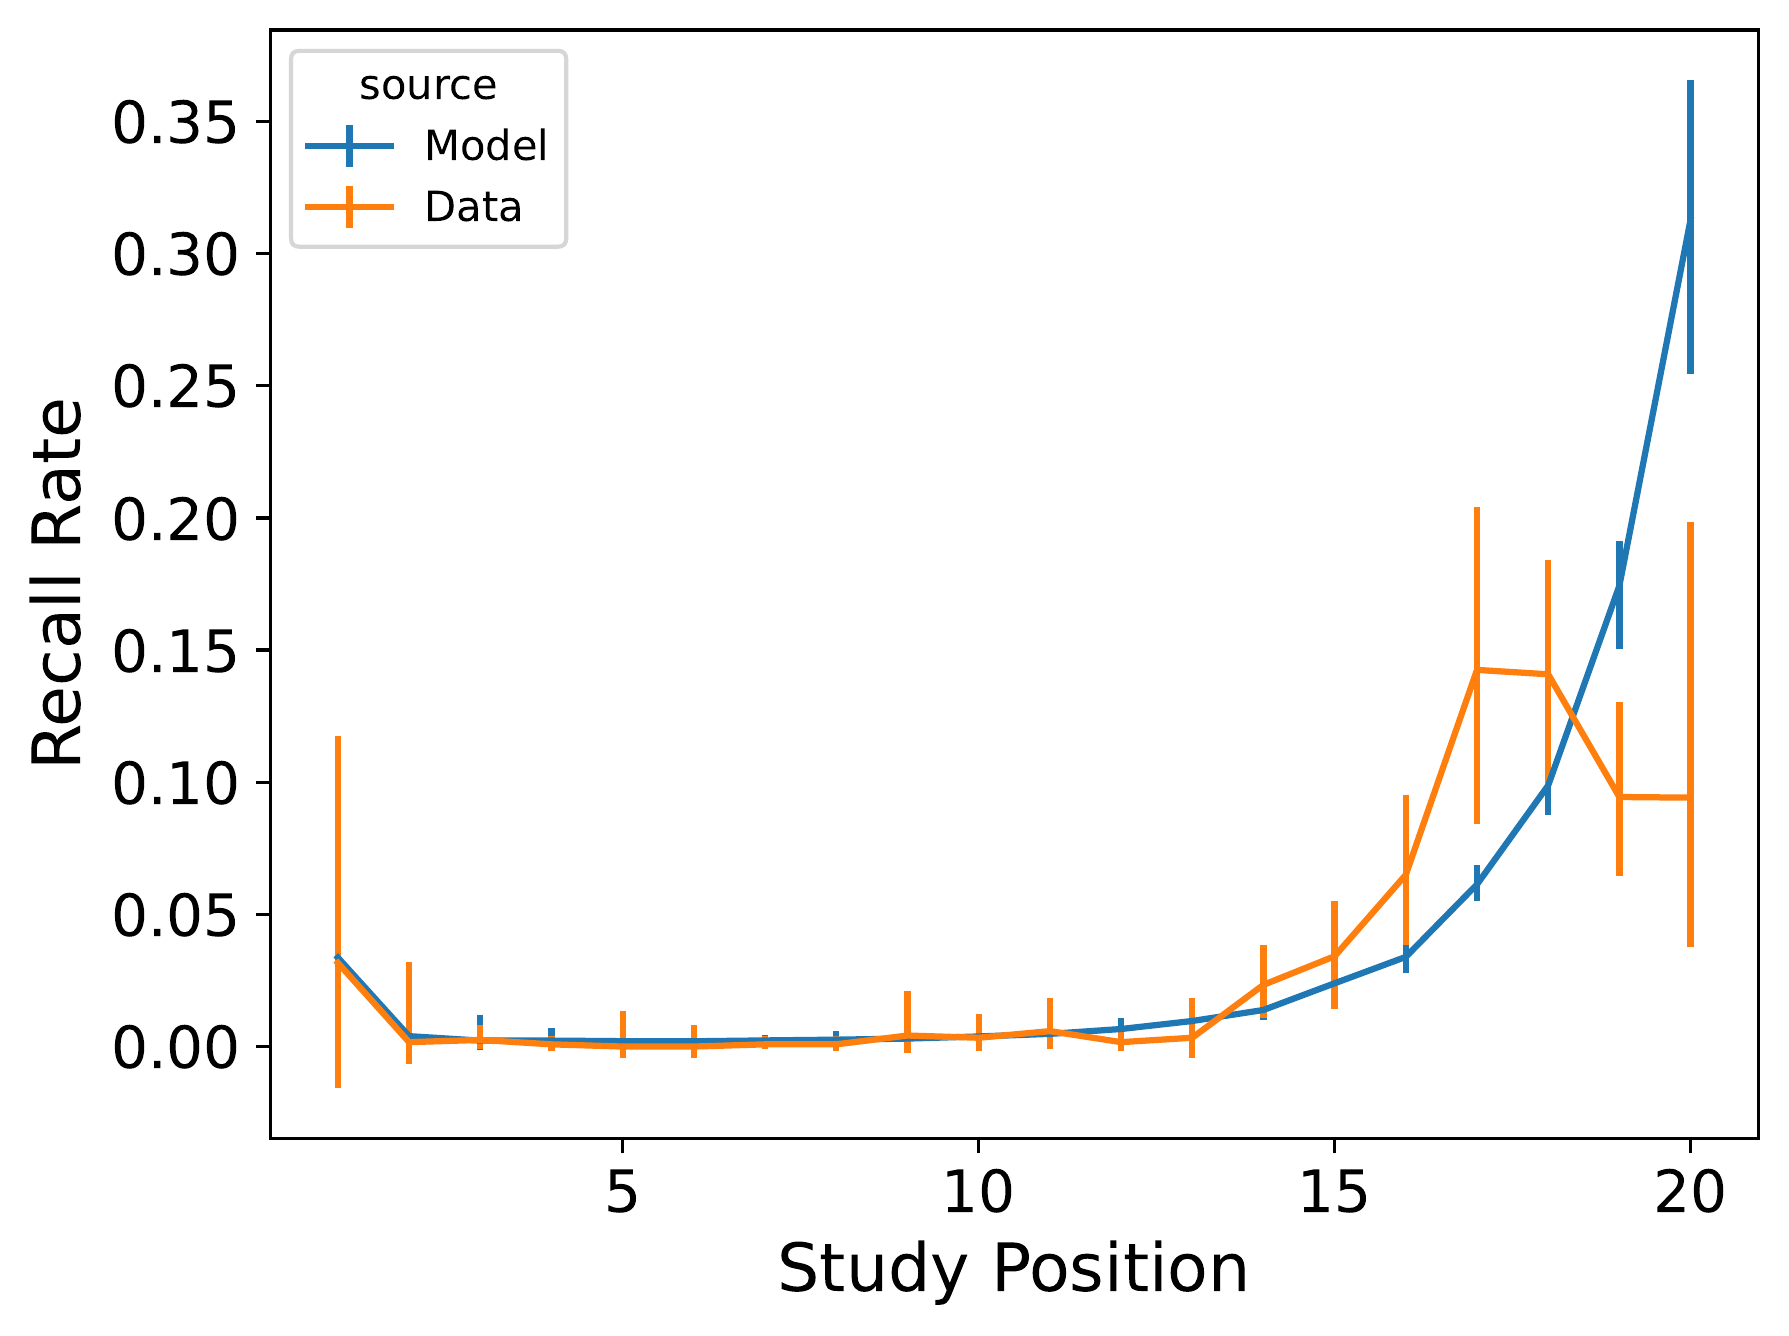
\includegraphics{icmr_figures/Murdock1962_ConnectionistCMR_Model_Fitting_LL20_pnr-1.png}\end{minipage}%
%
\begin{minipage}{0.33\linewidth}
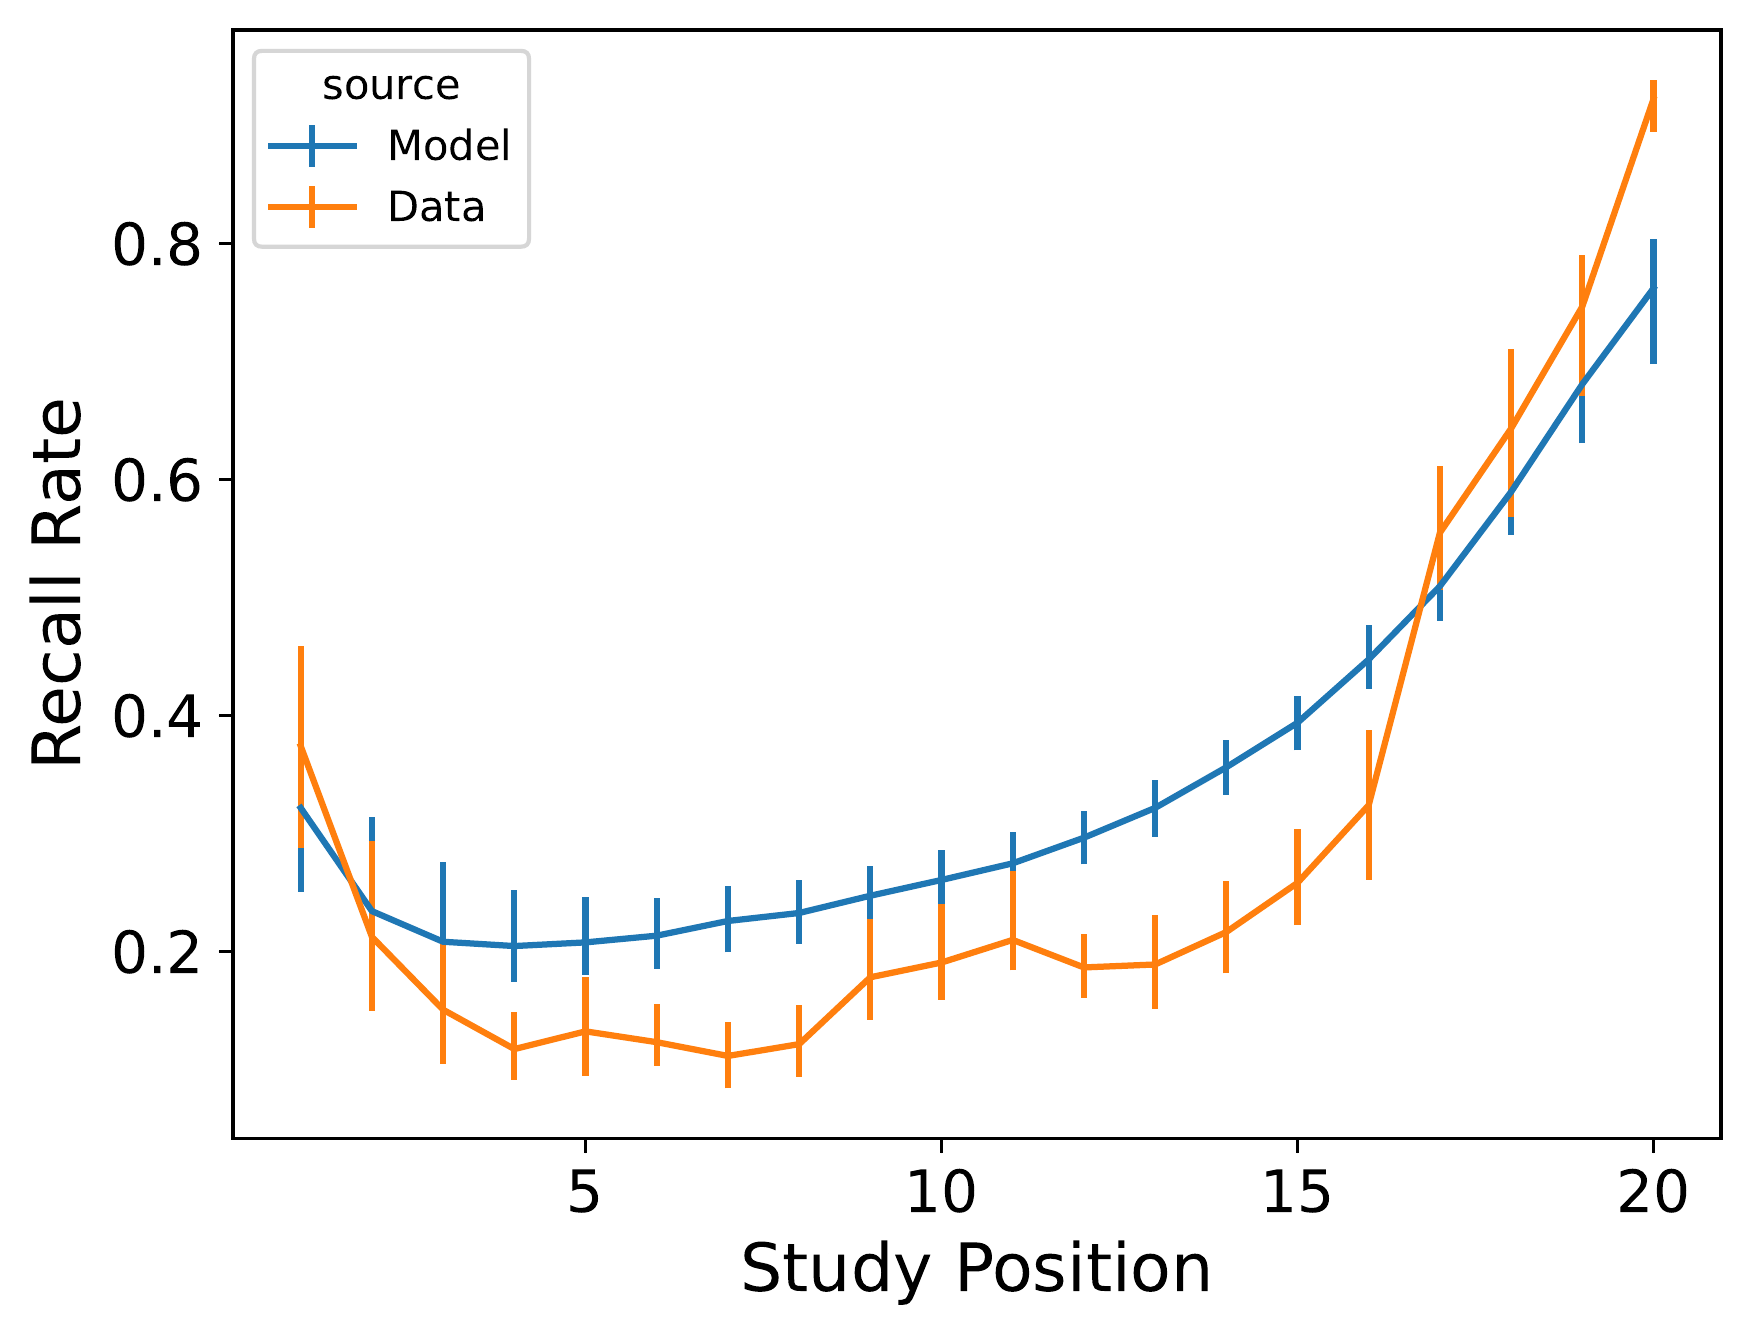
\includegraphics{icmr_figures/Murdock1962_ConnectionistCMR_Model_Fitting_LL20_spc-1.png}\end{minipage}%
\newline
\begin{minipage}{0.33\linewidth}
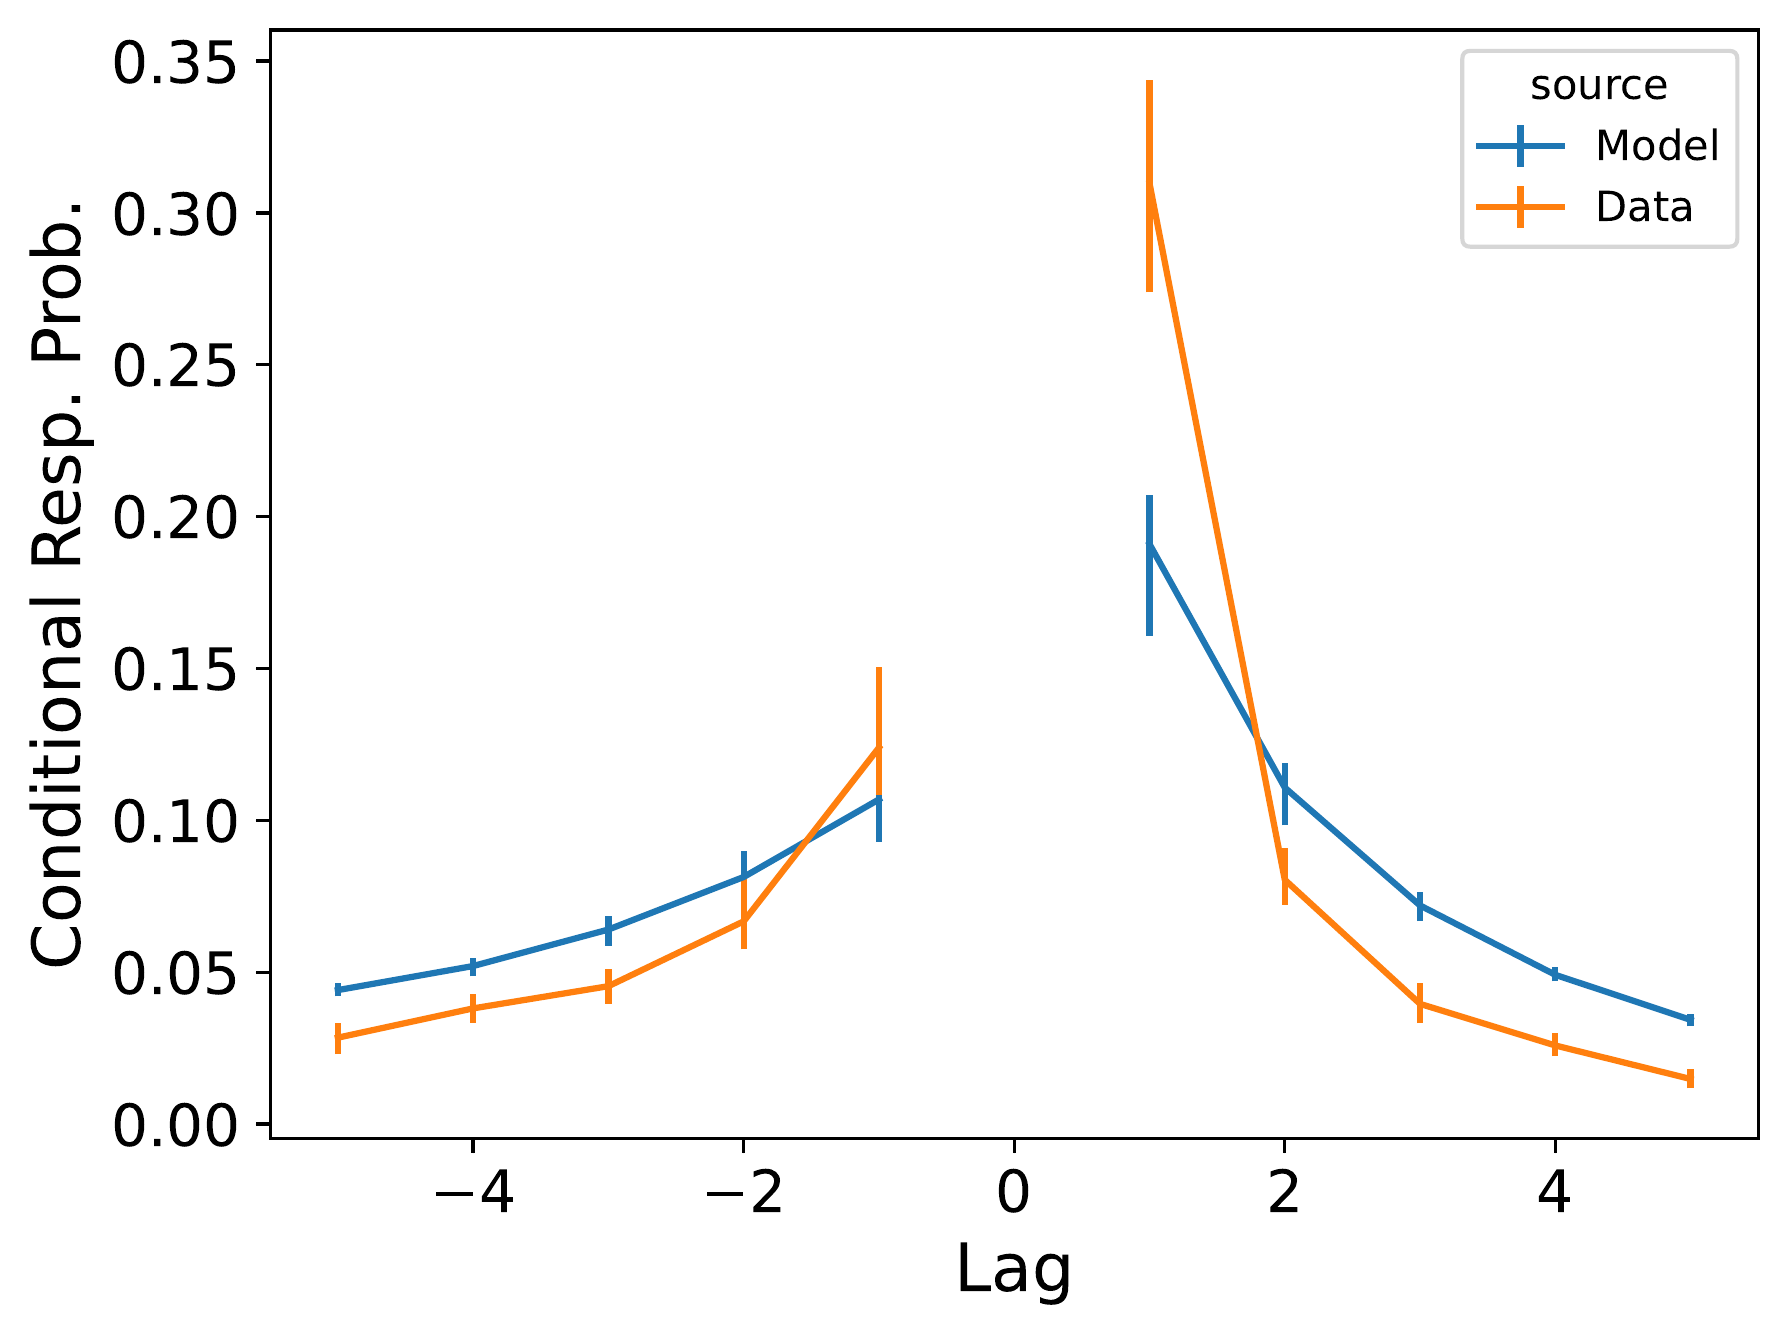
\includegraphics{icmr_figures/Murdock1962_InstanceCMR_Model_Fitting_LL20_crp-1.png}\end{minipage}%
%
\begin{minipage}{0.33\linewidth}
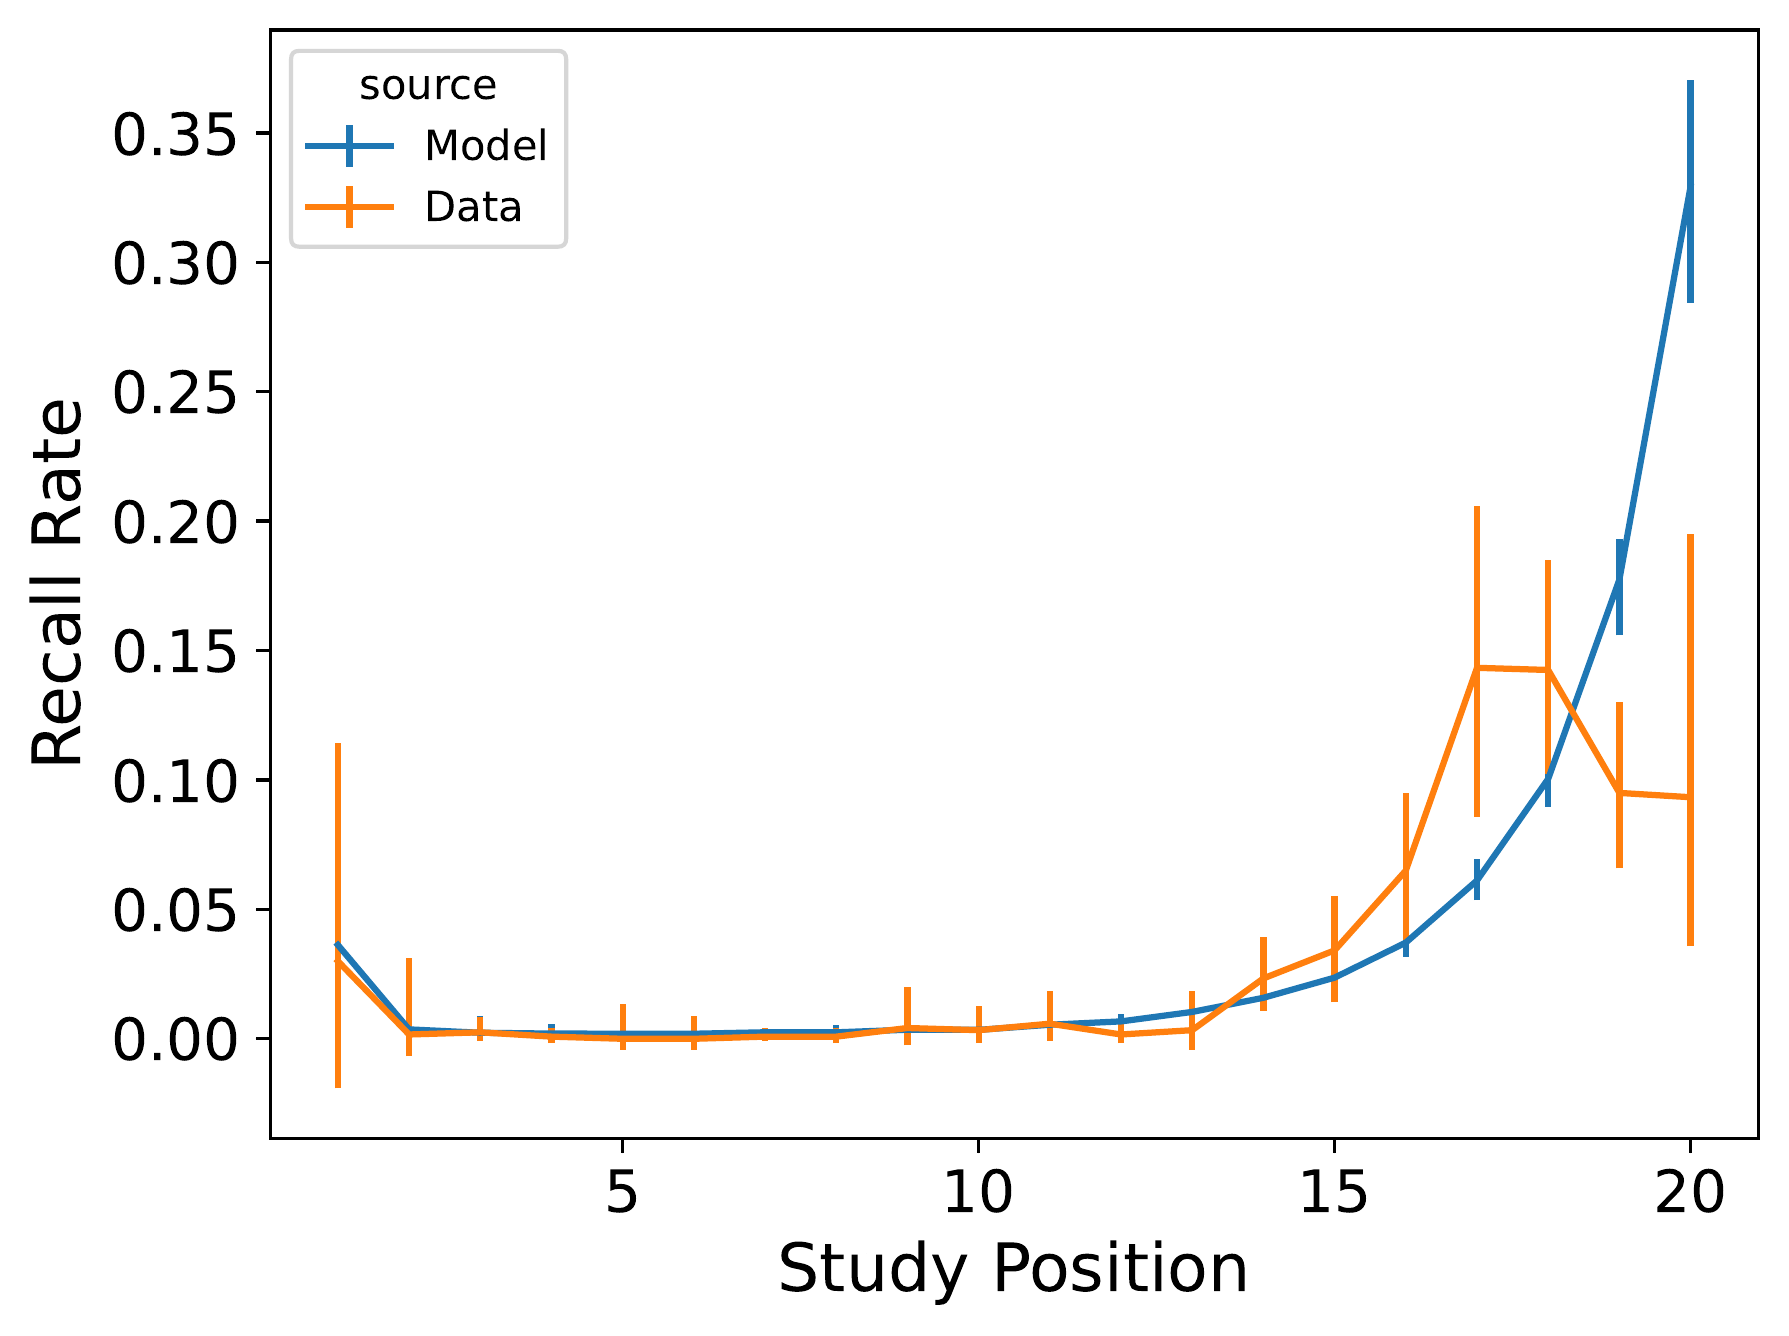
\includegraphics{icmr_figures/Murdock1962_InstanceCMR_Model_Fitting_LL20_pnr-1.png}\end{minipage}%
%
\begin{minipage}{0.33\linewidth}
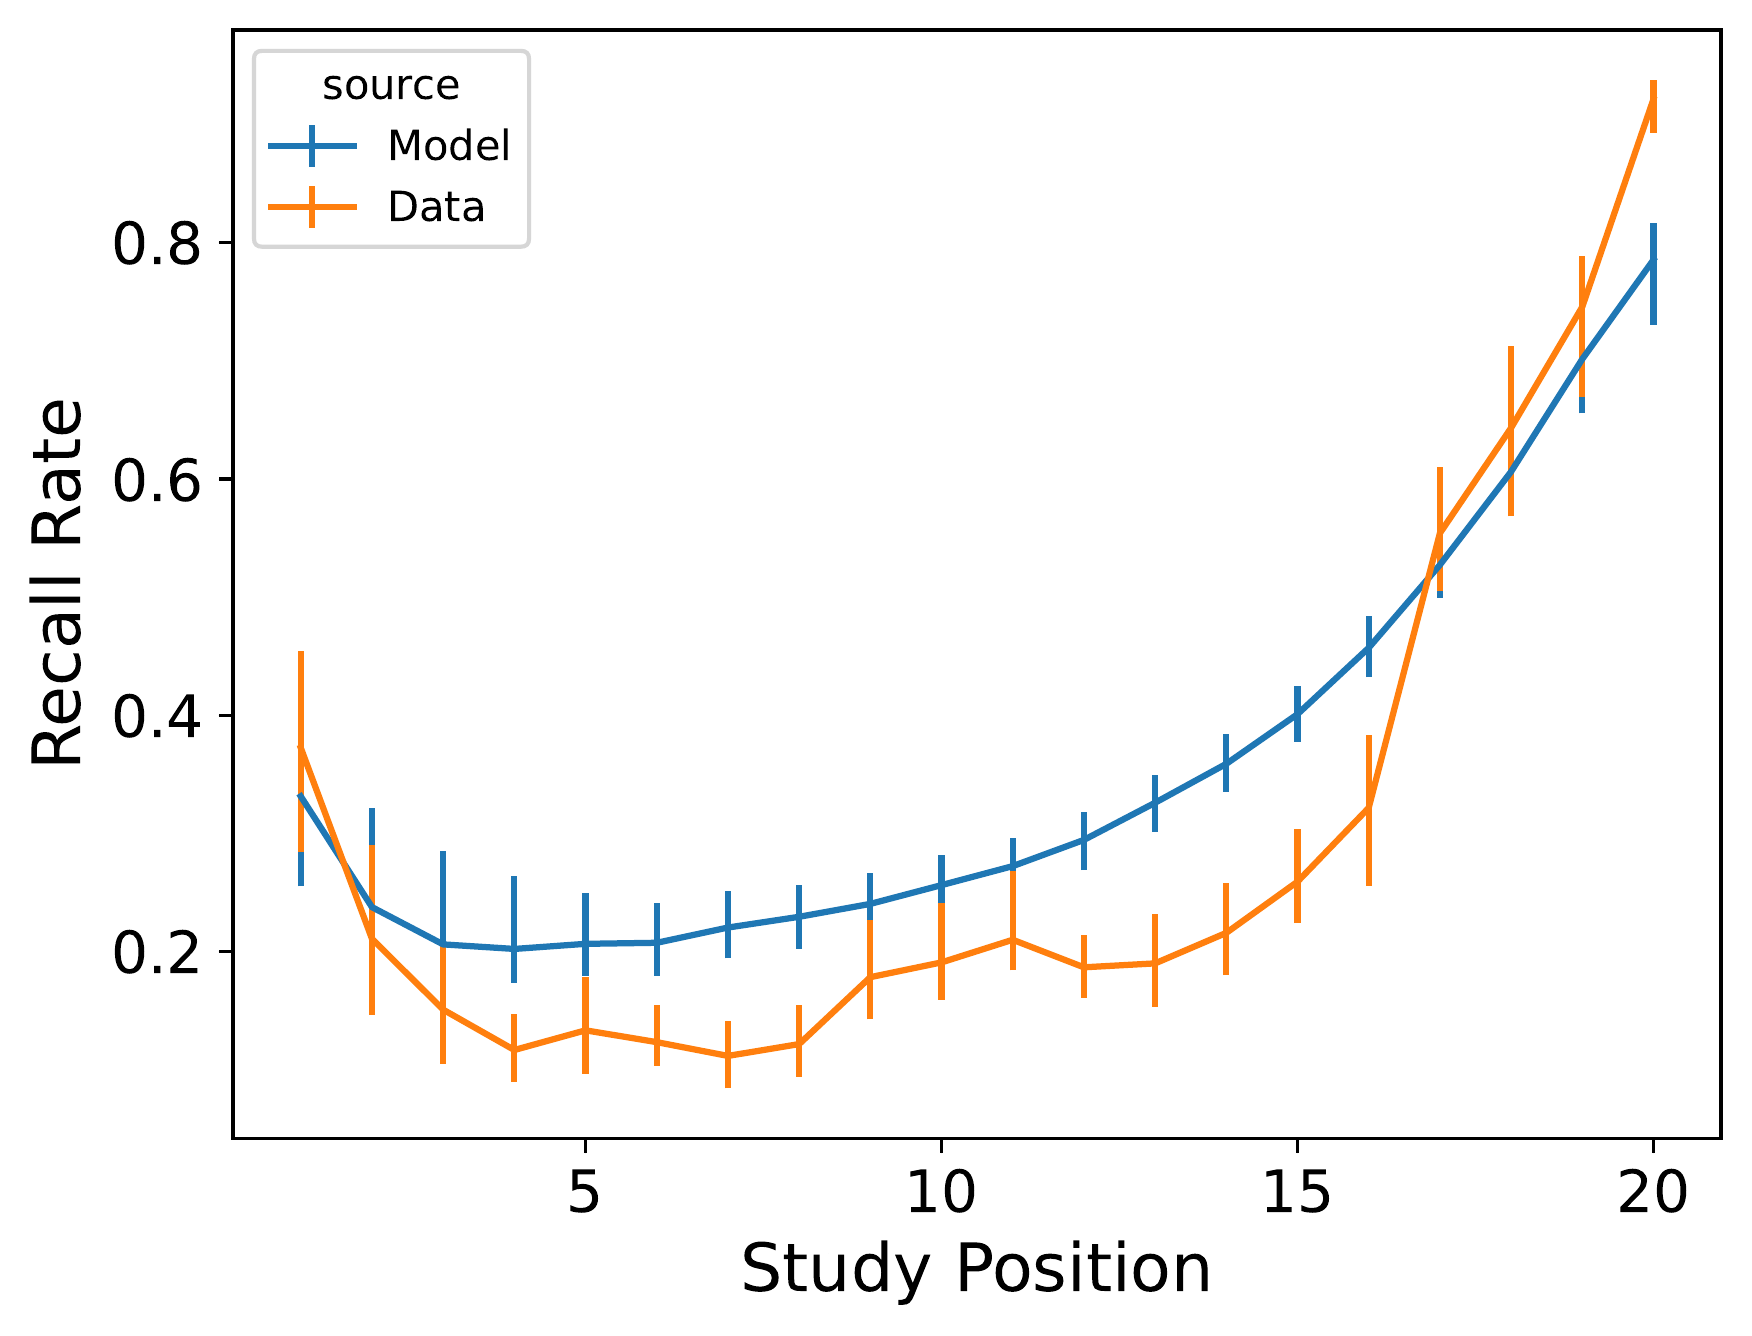
\includegraphics{icmr_figures/Murdock1962_InstanceCMR_Model_Fitting_LL20_spc-1.png}\end{minipage}%
\newline
\begin{minipage}{0.33\linewidth}
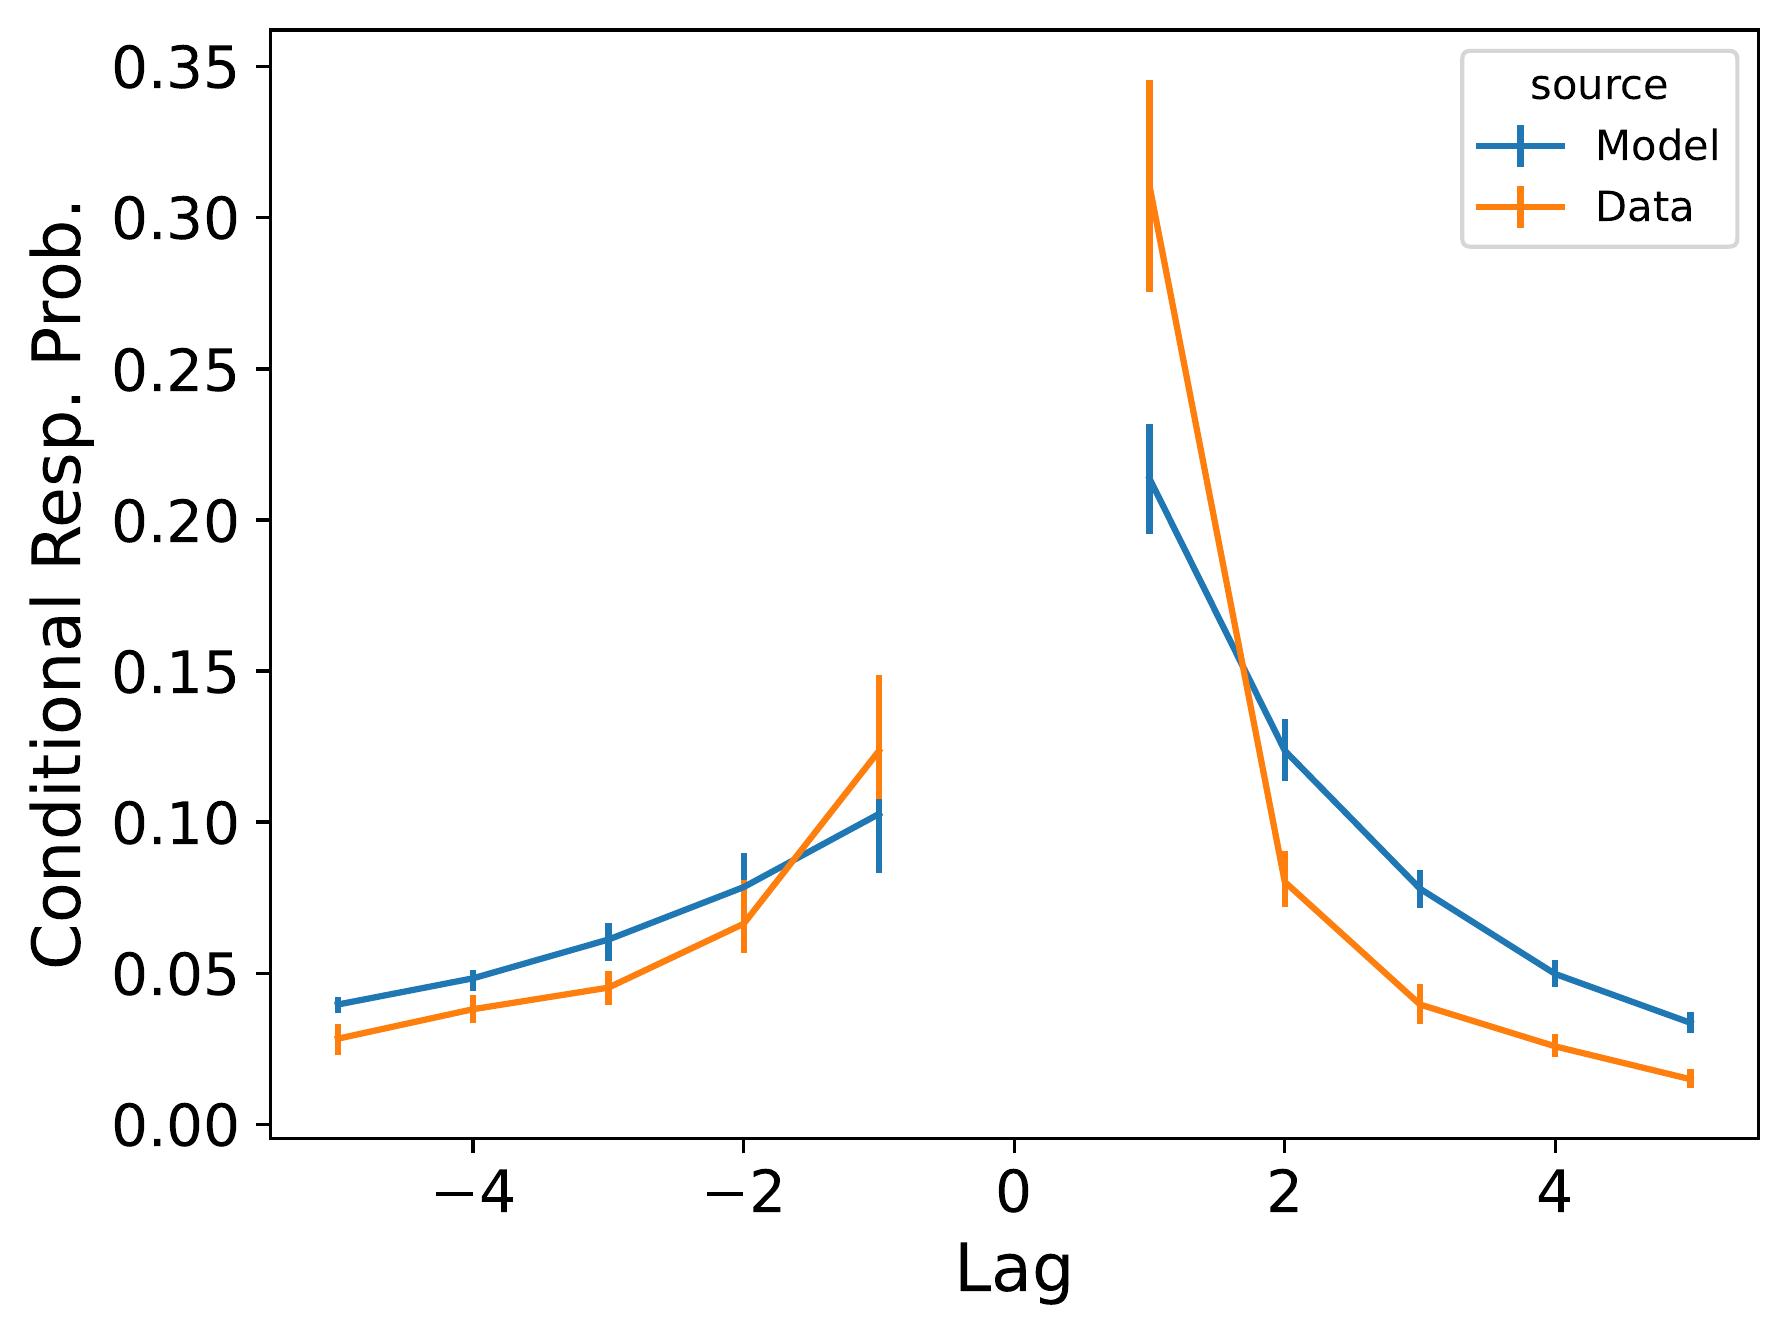
\includegraphics{icmr_figures/Murdock1962_TraceScalingCMR_Model_Fitting_LL20_crp-1.png}\end{minipage}%
%
\begin{minipage}{0.33\linewidth}
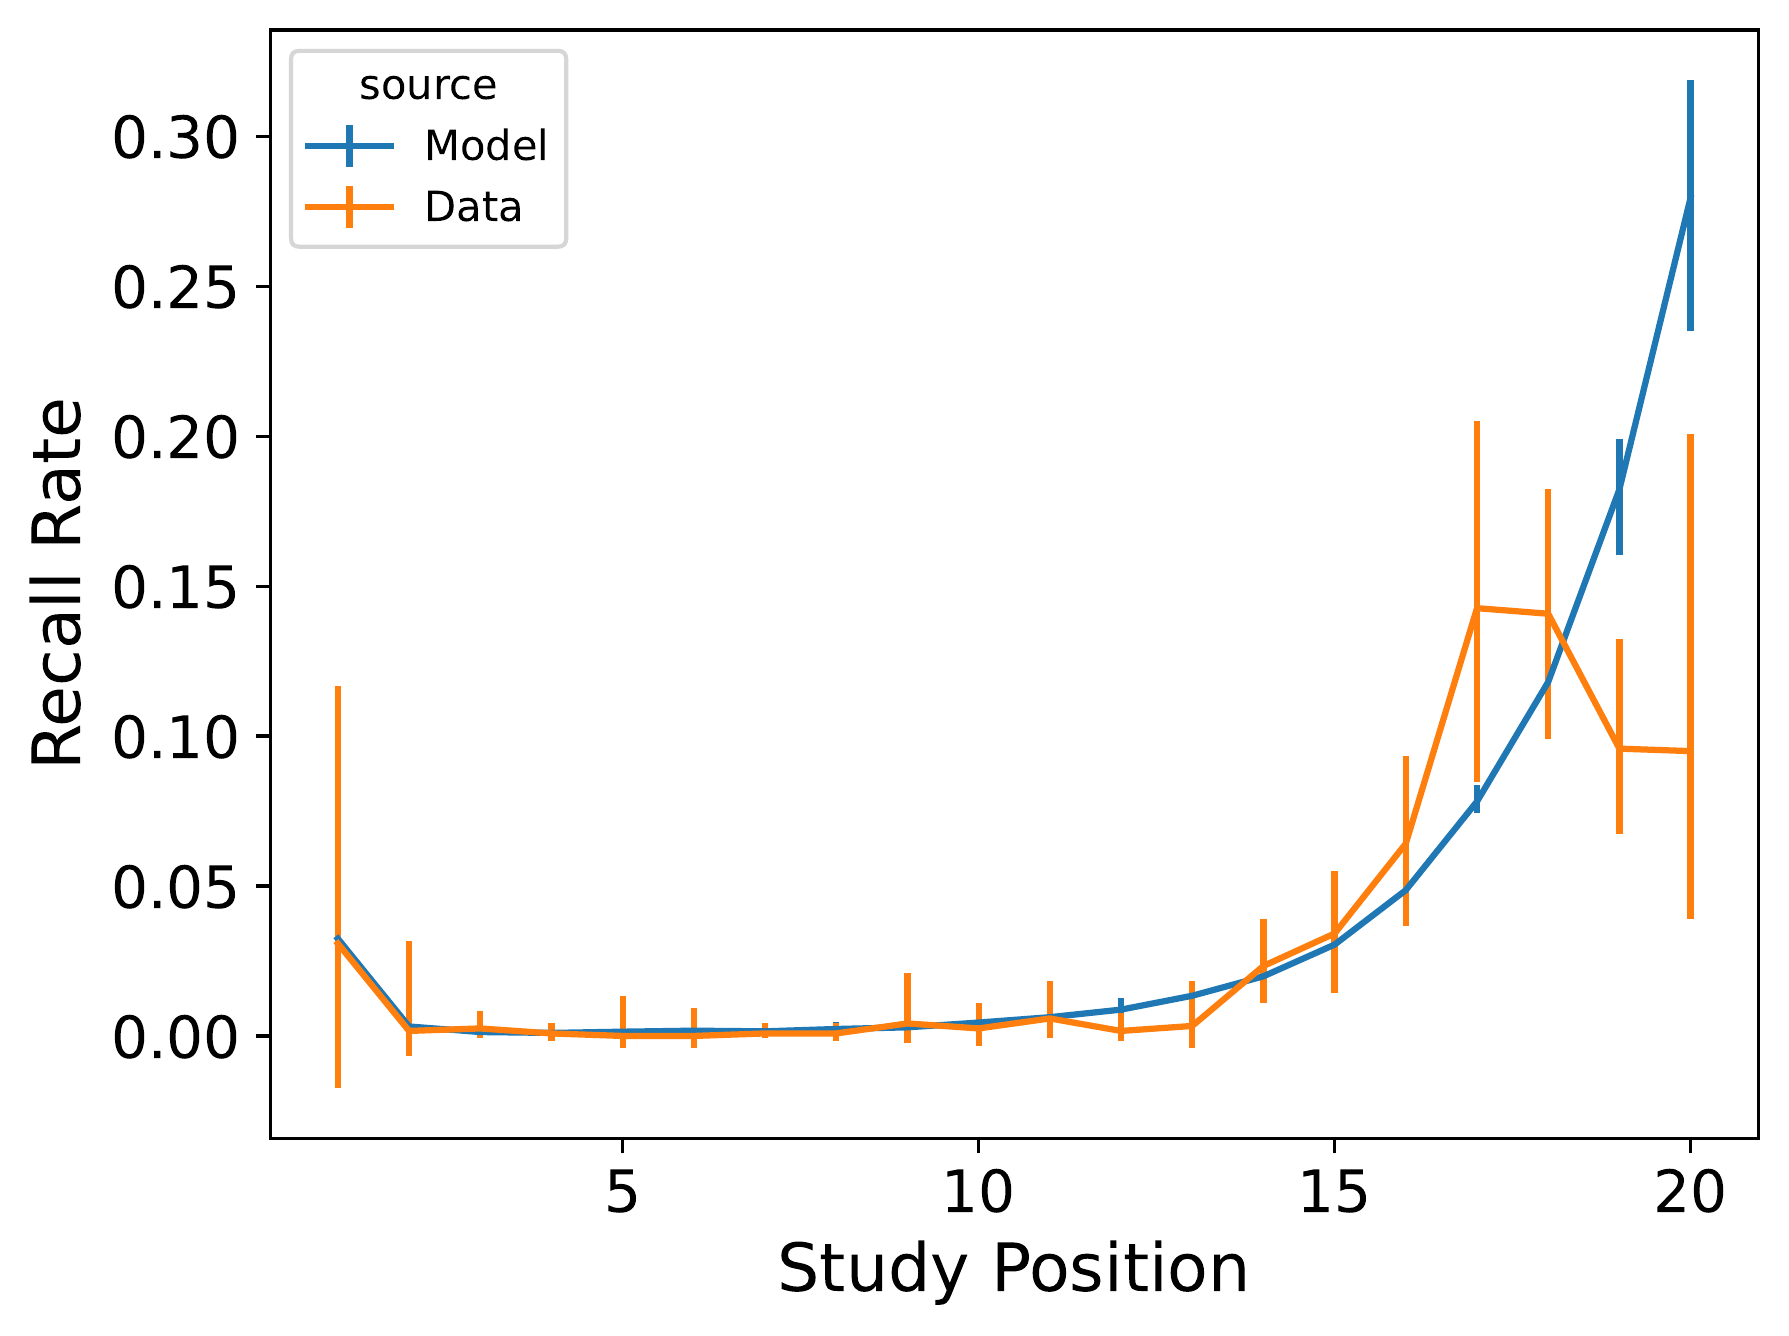
\includegraphics{icmr_figures/Murdock1962_TraceScalingCMR_Model_Fitting_LL20_pnr-1.png}\end{minipage}%
%
\begin{minipage}{0.33\linewidth}
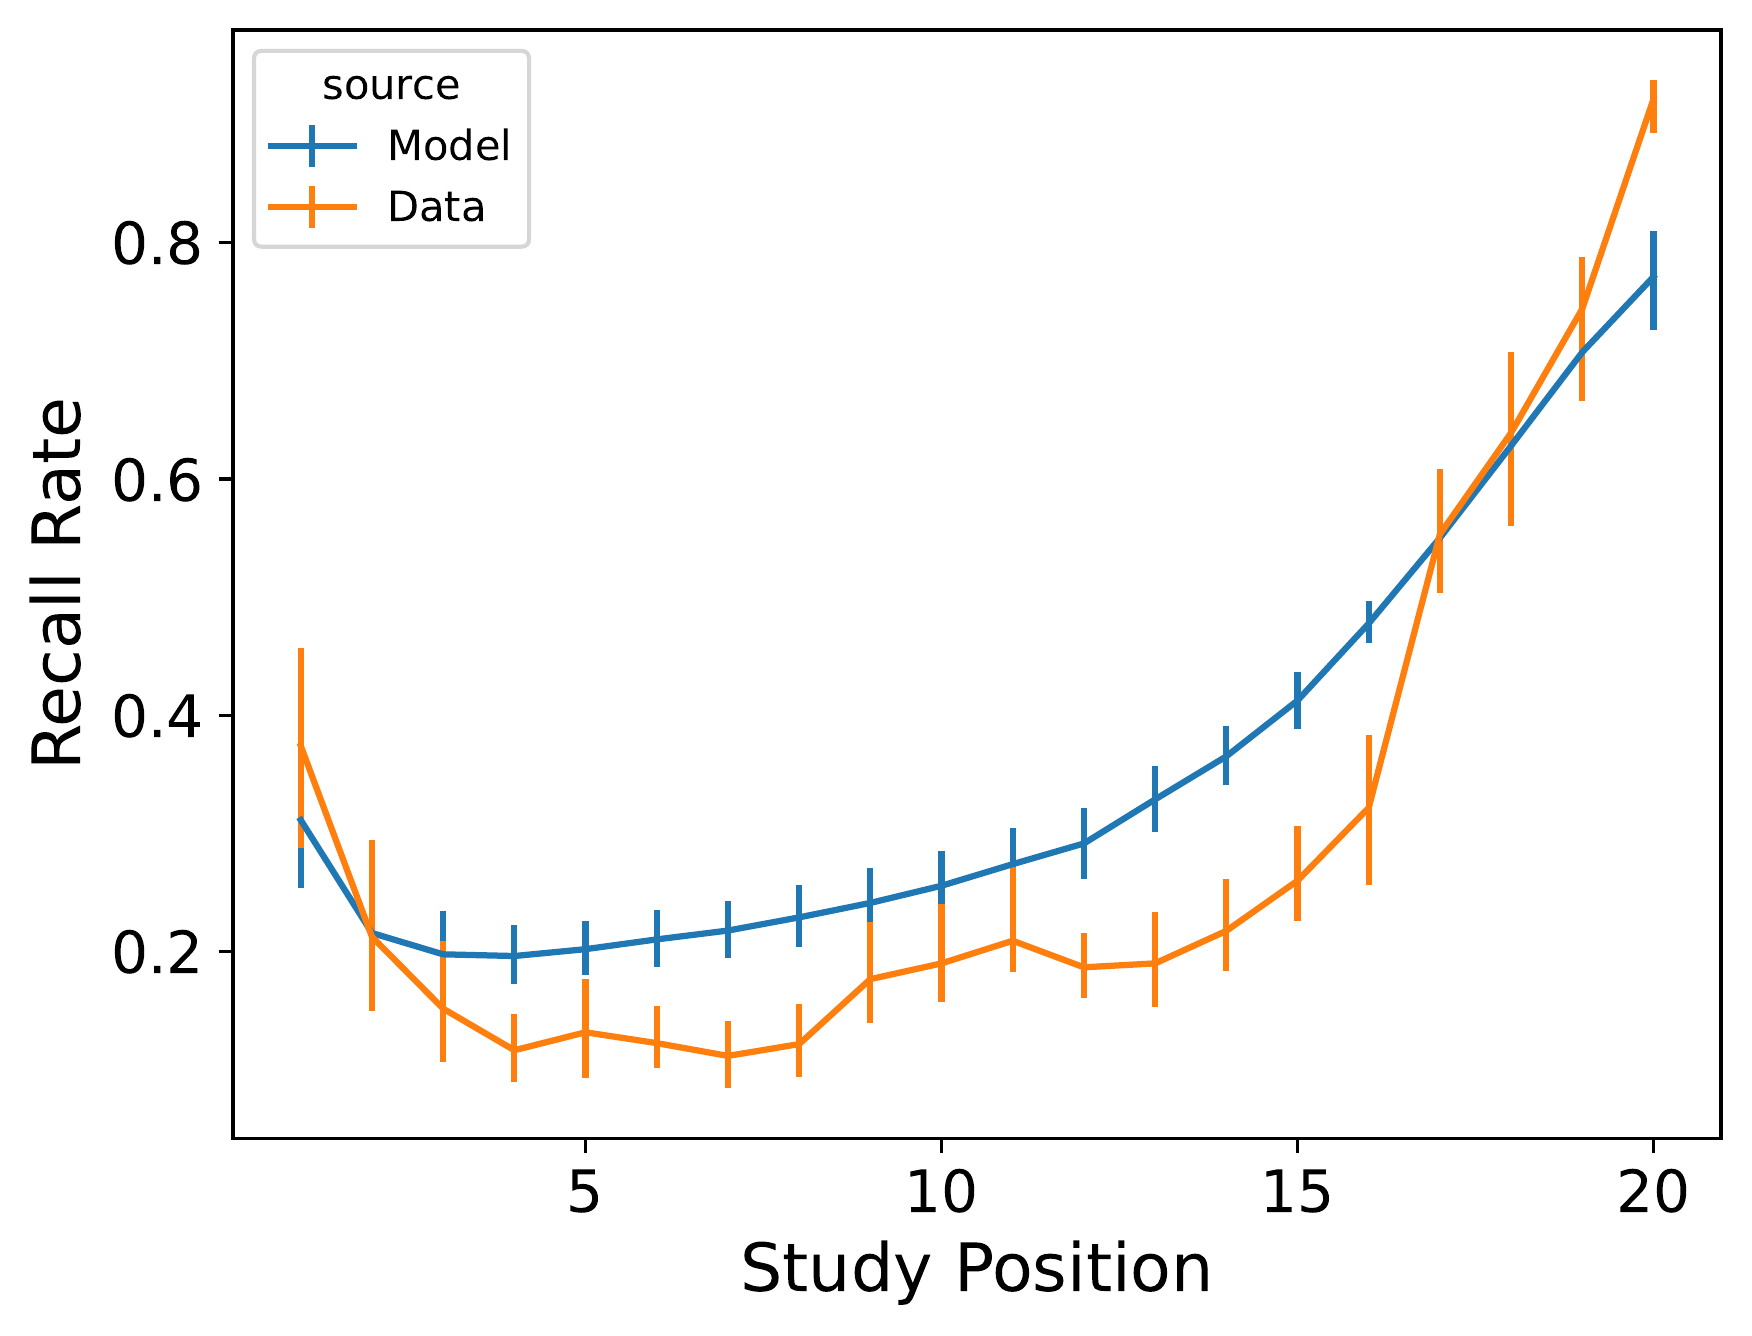
\includegraphics{icmr_figures/Murdock1962_TraceScalingCMR_Model_Fitting_LL20_spc-1.png}\end{minipage}%
\newline
\begin{minipage}{0.33\linewidth}
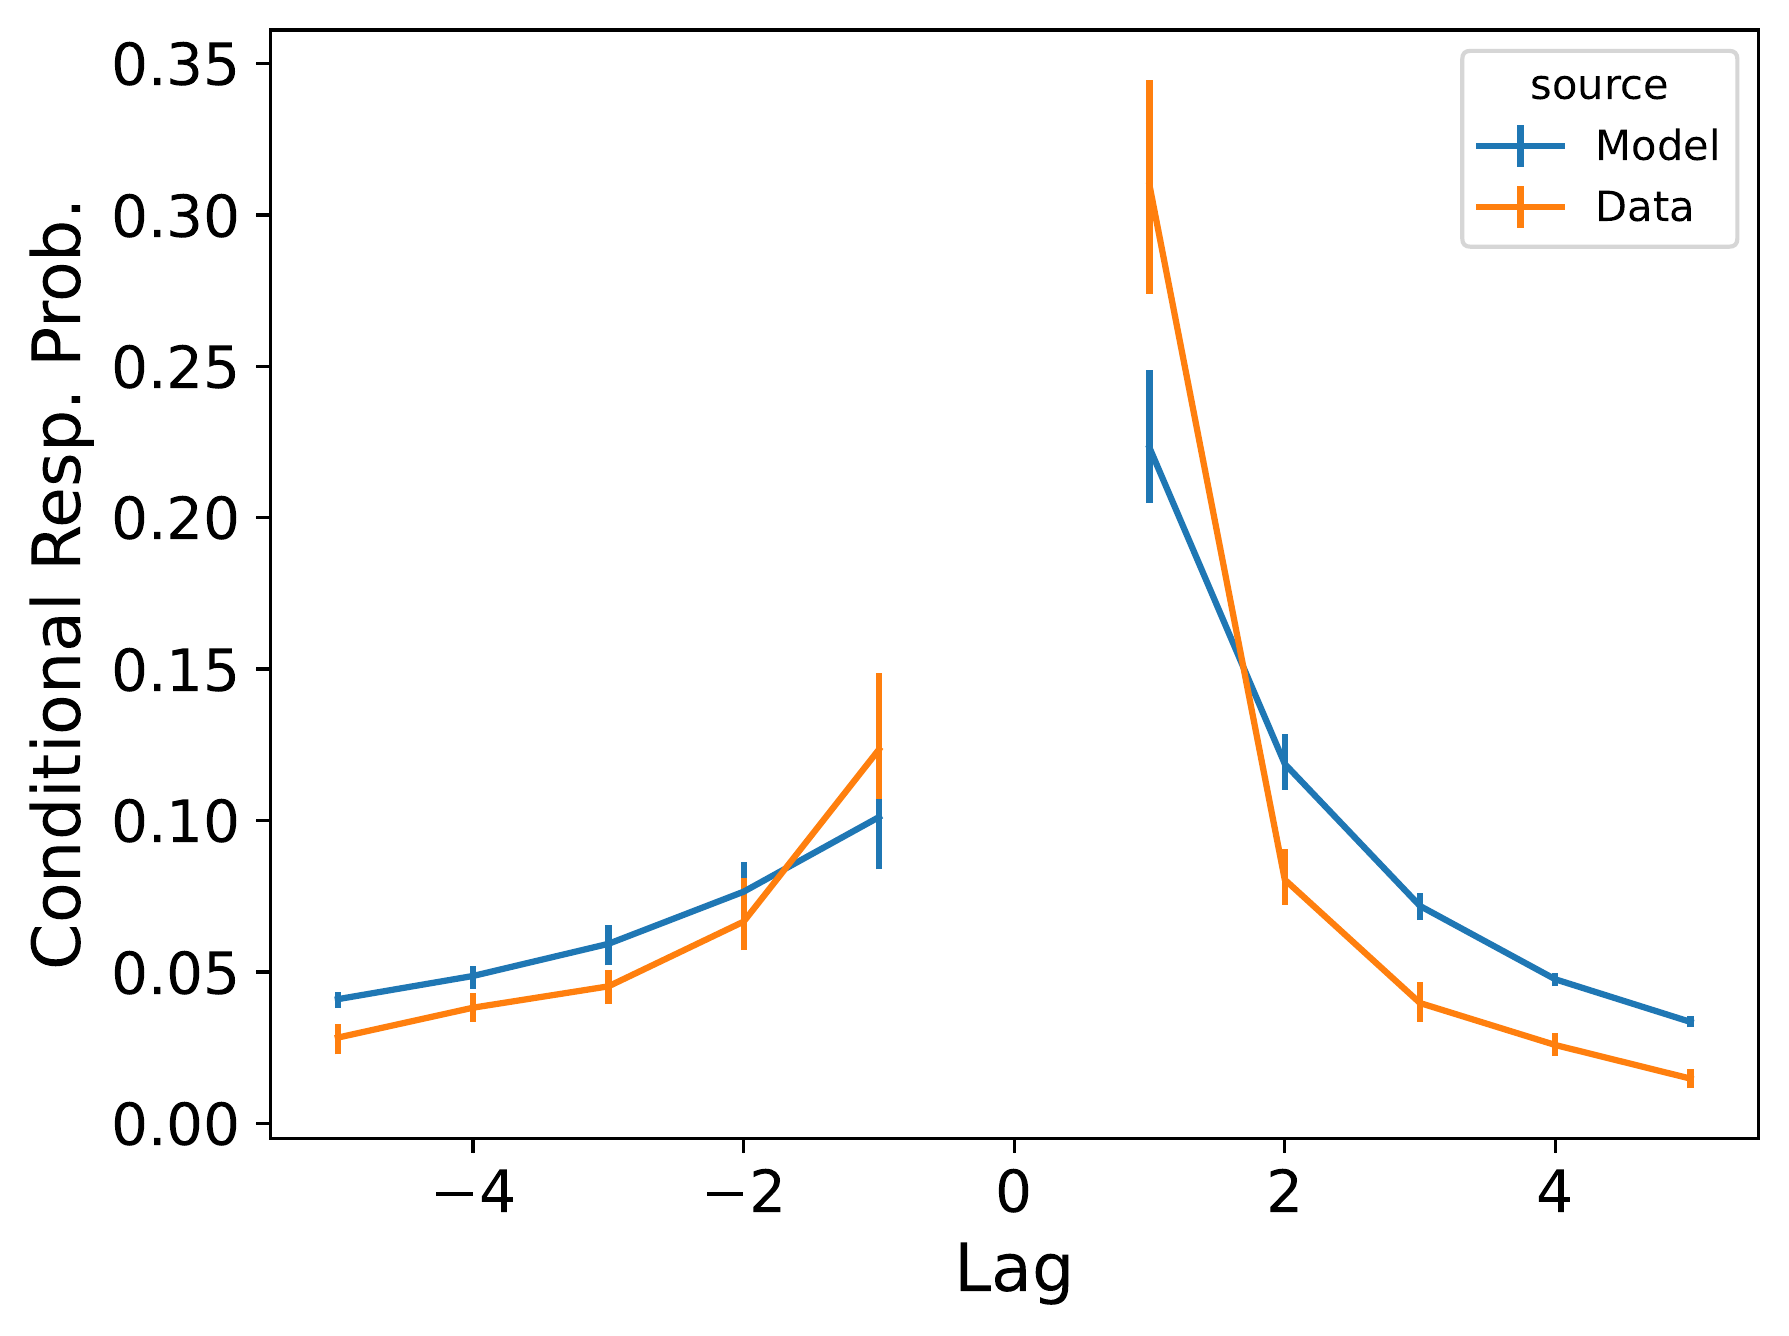
\includegraphics{icmr_figures/Murdock1962_MultiScalingCMR_Model_Fitting_LL20_crp-1.png}\end{minipage}%
%
\begin{minipage}{0.33\linewidth}
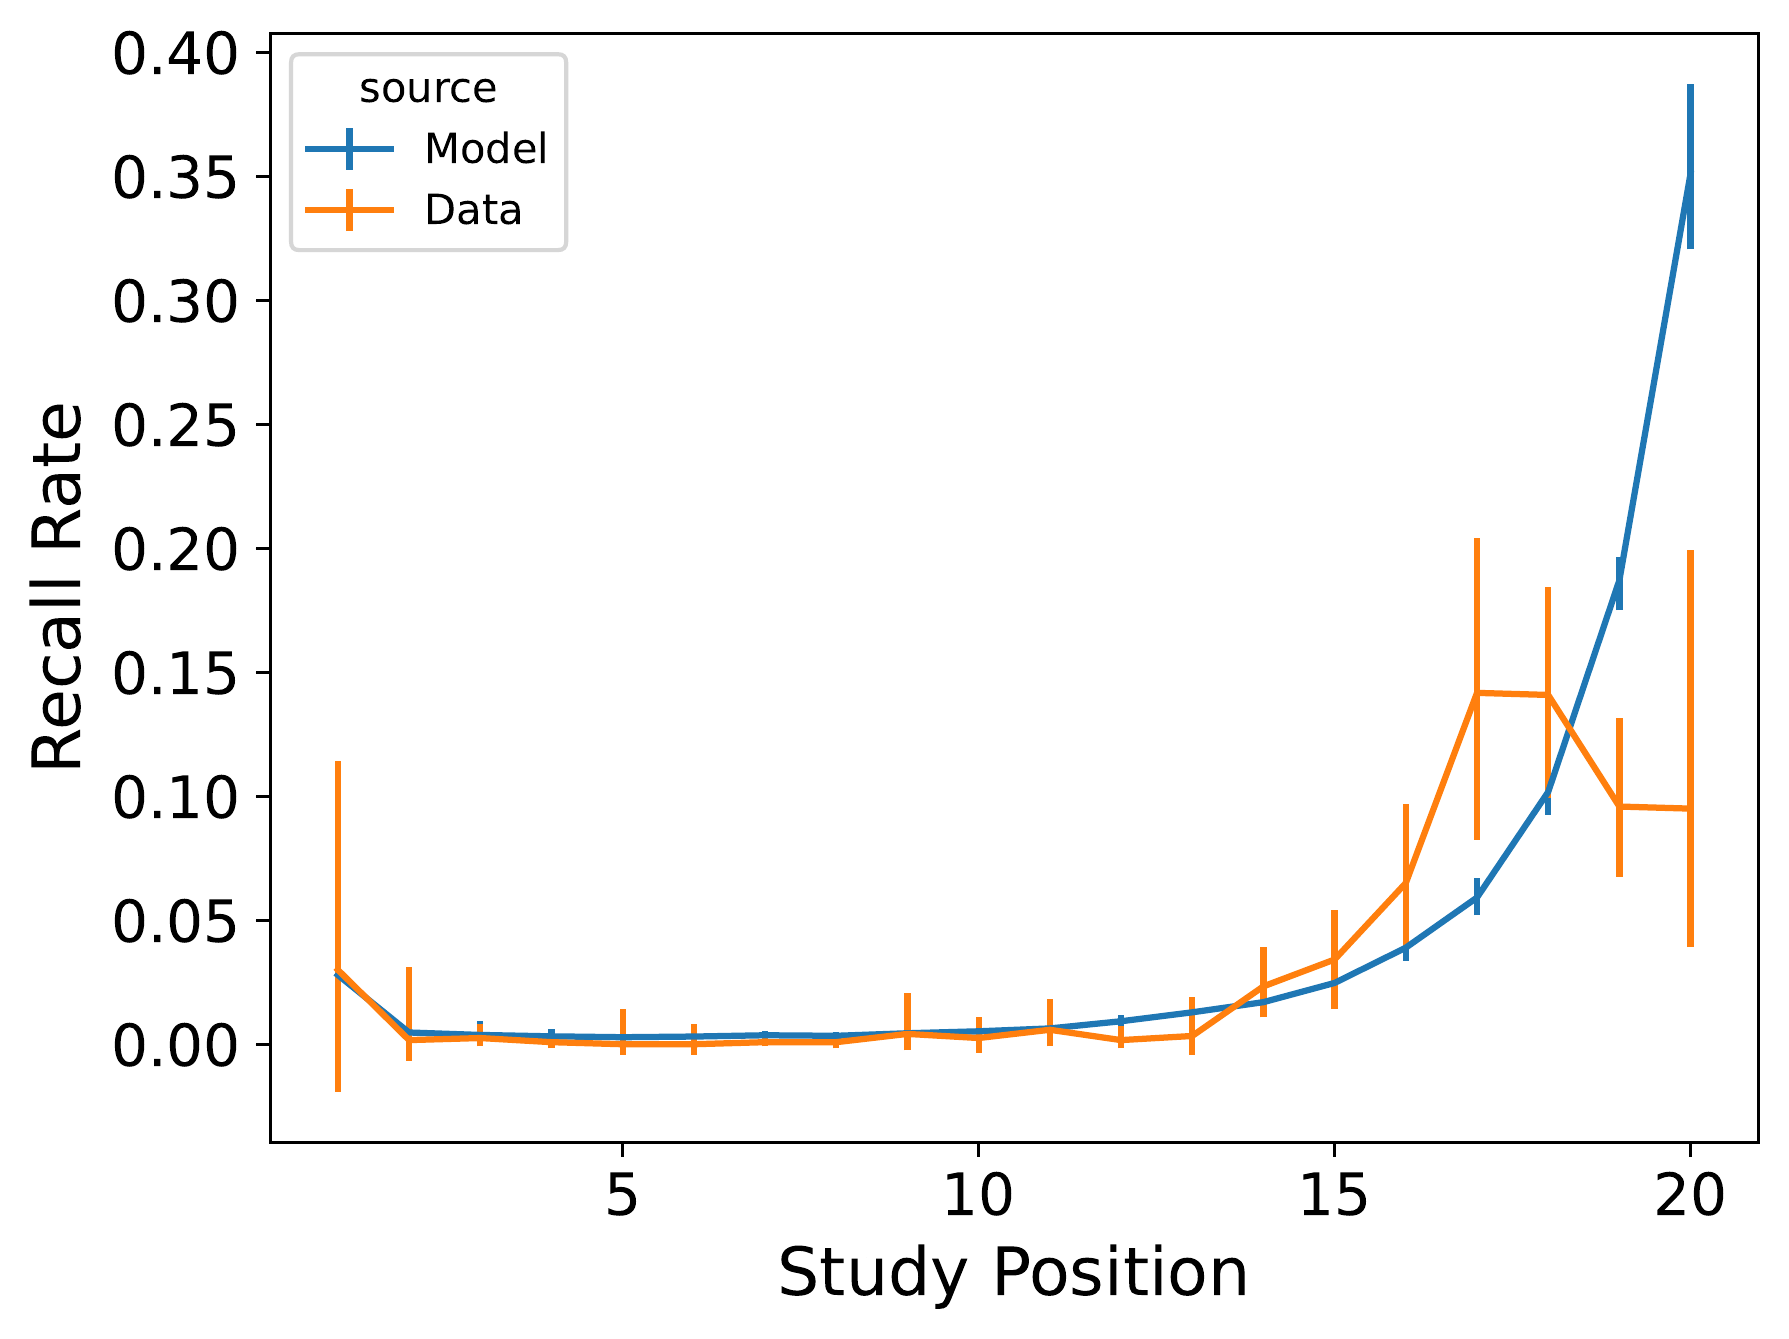
\includegraphics{icmr_figures/Murdock1962_MultiScalingCMR_Model_Fitting_LL20_pnr-1.png}\end{minipage}%
%
\begin{minipage}{0.33\linewidth}
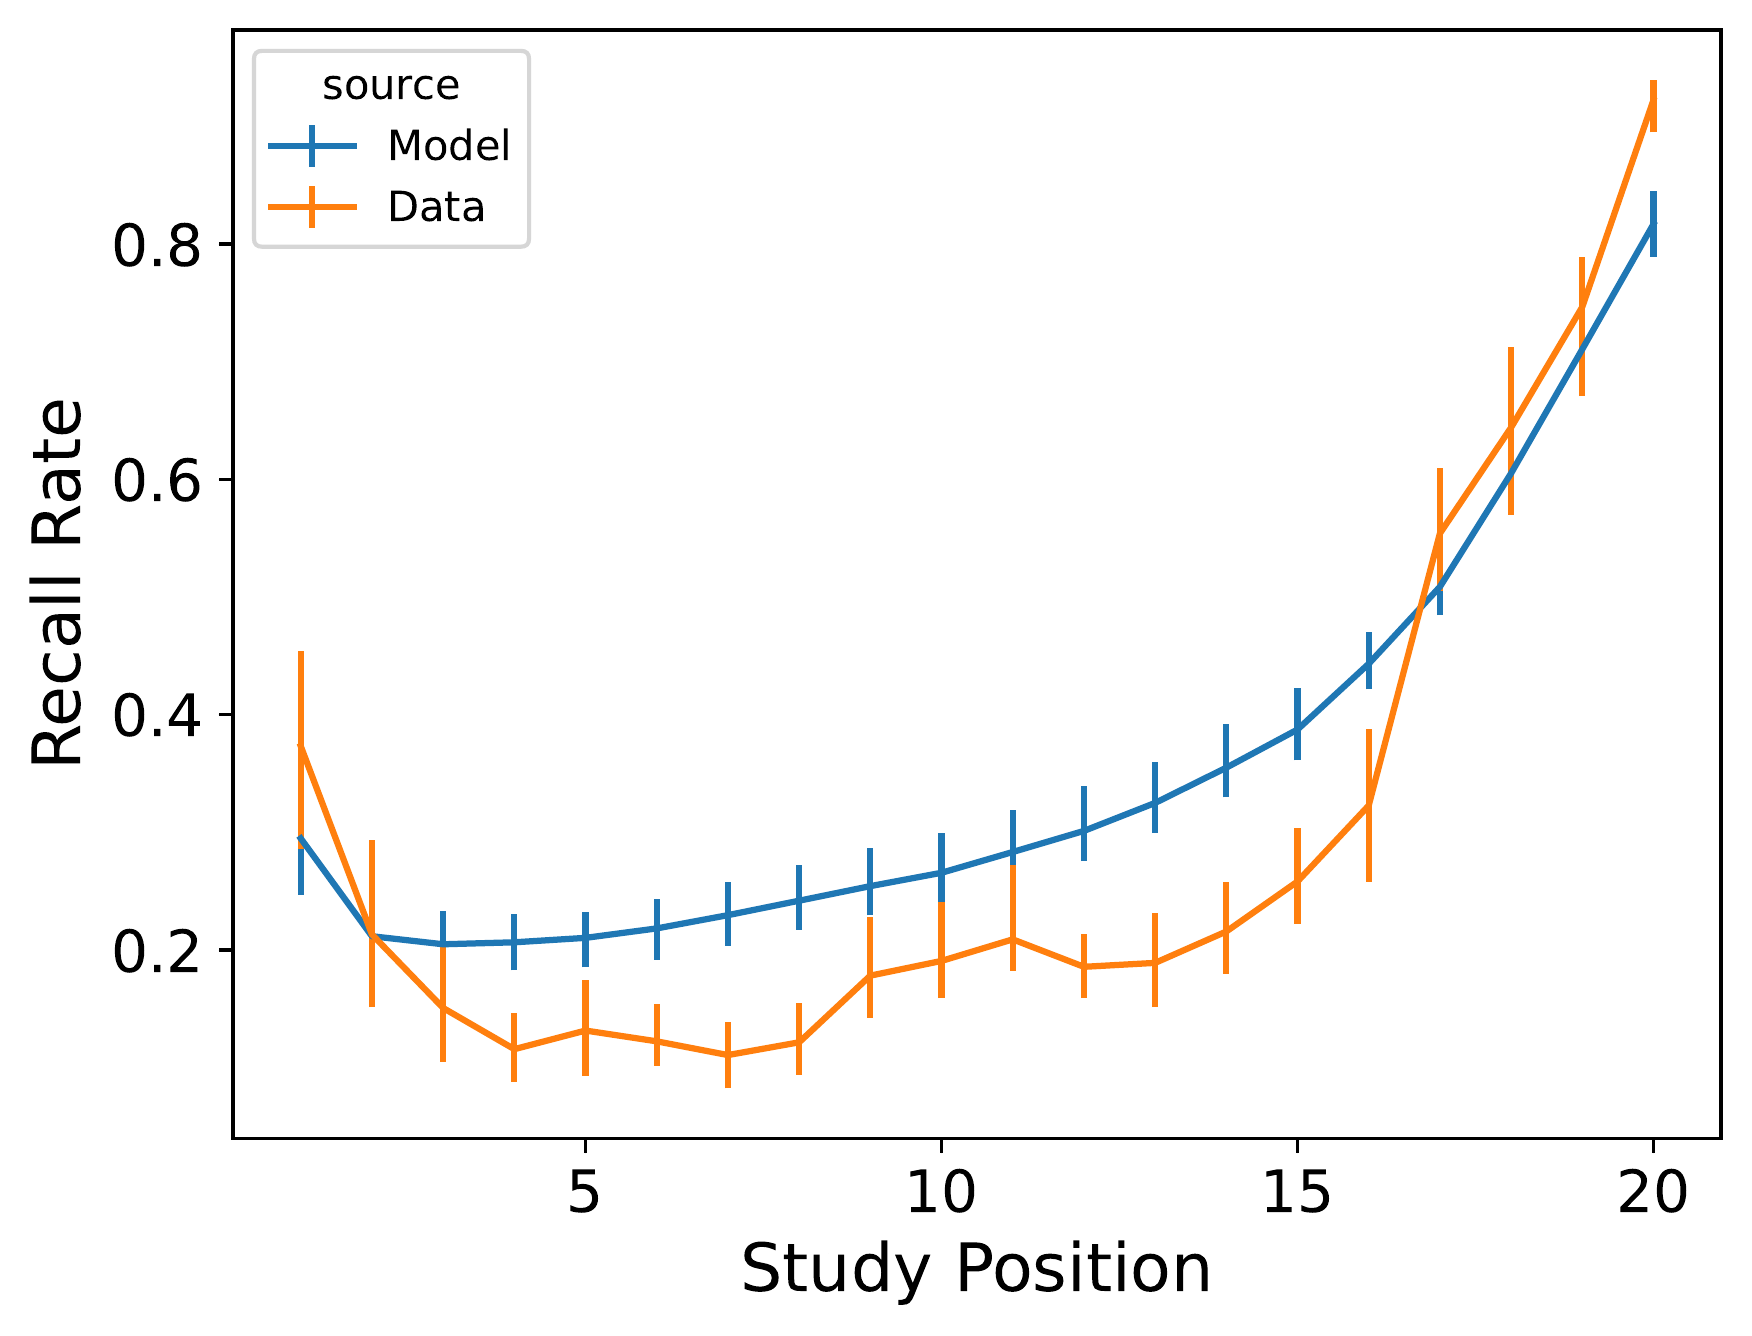
\includegraphics{icmr_figures/Murdock1962_MultiScalingCMR_Model_Fitting_LL20_spc-1.png}\end{minipage}%

\caption{\label{fig-murdock1962memory20}Summary statistic fits to
Murdock Jr (1962) where list length = 20. Top: Connectionist CMR. Second
Row: Instance CMR, \(\tau_{t}\) set to 1. Third Row: Trace Scaling CMR
-- Instance CMR, \(\tau_{c}\) set to 1 and \(\tau_{t}\) optimized during
fitting. Fourth Row: Multi Scaling CMR -- Instance CMR, both
\(\tau_{t}\) and \(\tau_c\) optimized during fitting. Left: conditional
response probability as a function of lag. Middle: probability of
starting recall with each serial position. Right: recall probability as
a function of serial position.}

\end{figure}%

\begin{figure}

\begin{minipage}{0.33\linewidth}
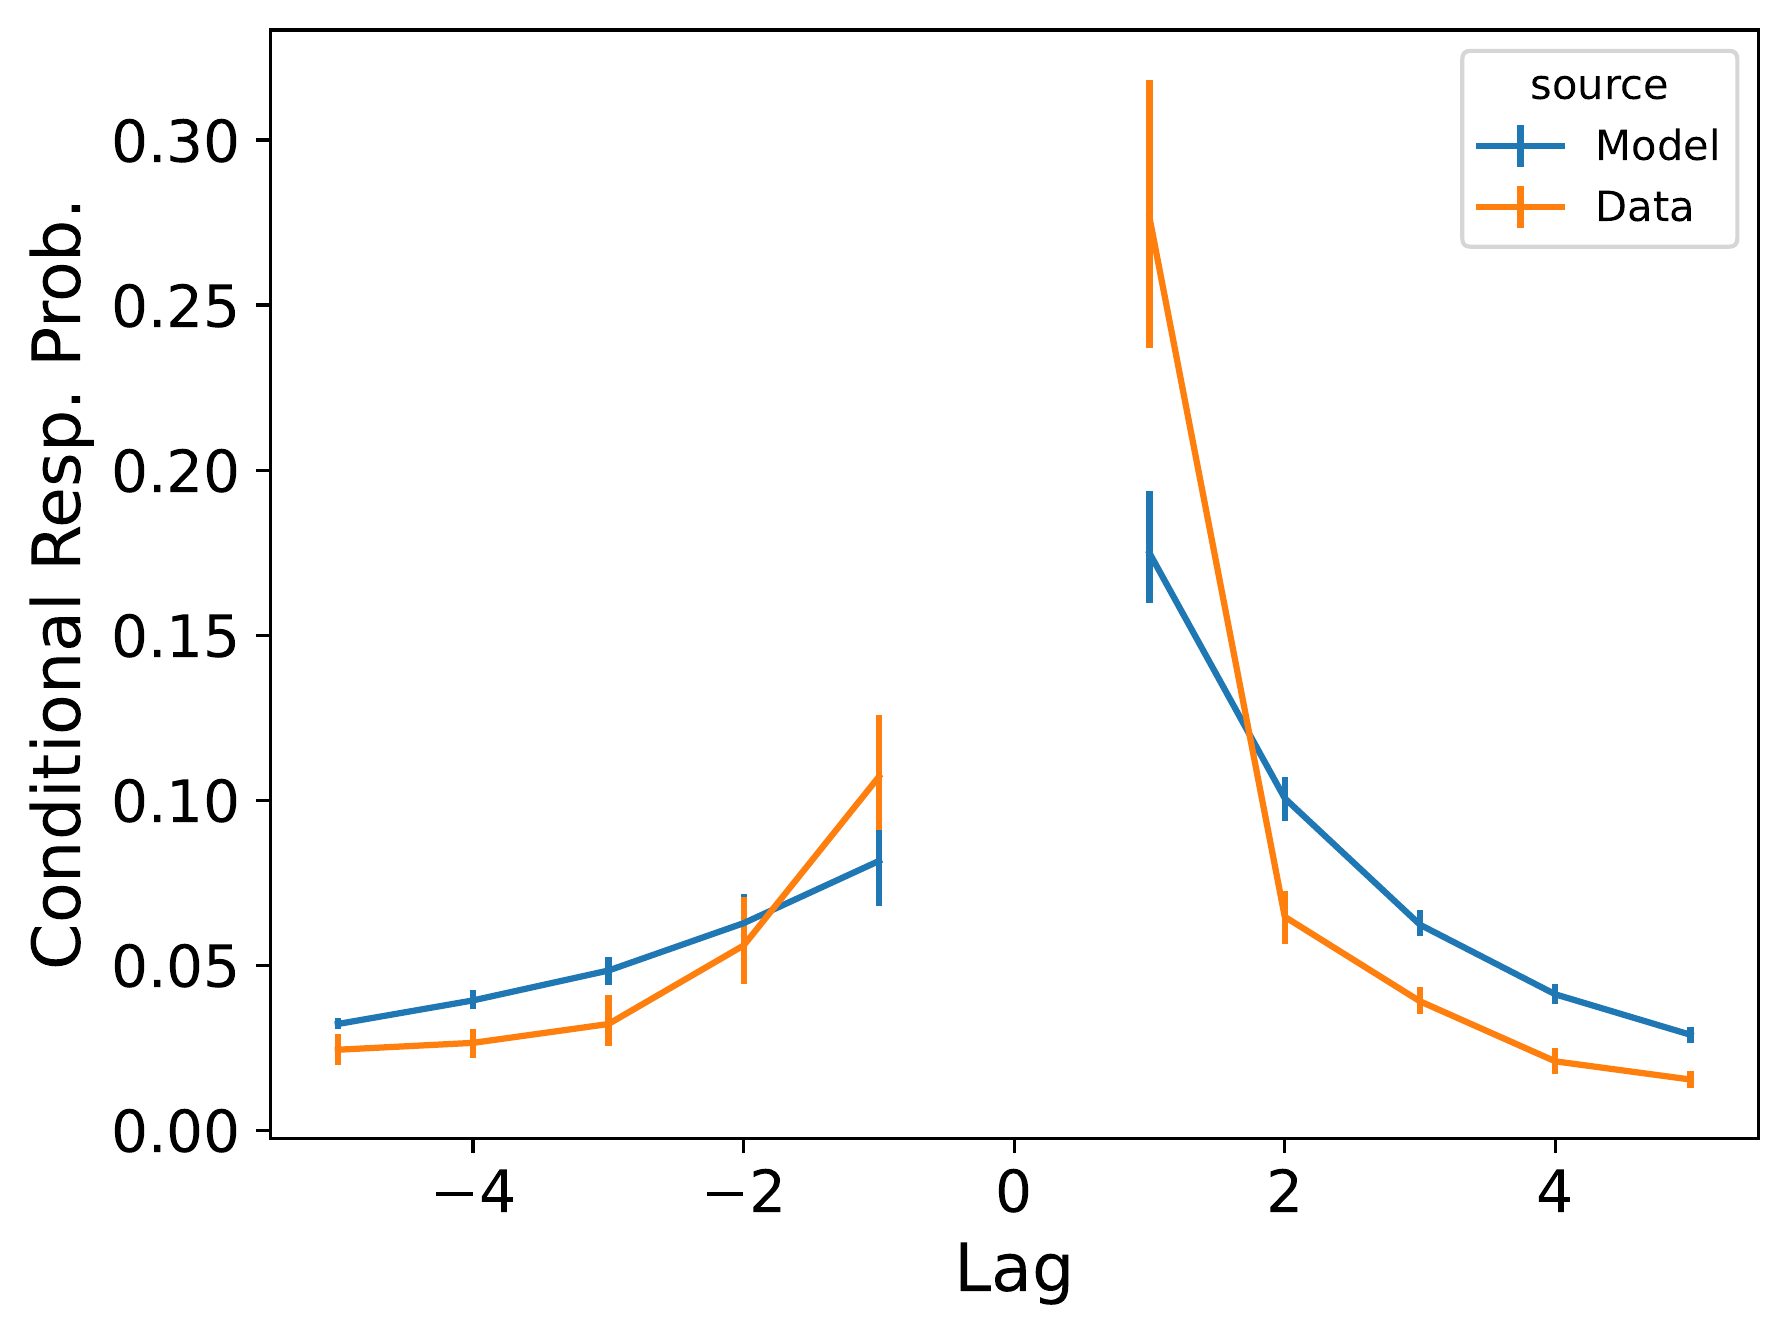
\includegraphics{icmr_figures/Murdock1962_ConnectionistCMR_Model_Fitting_LL30_crp-1.png}\end{minipage}%
%
\begin{minipage}{0.33\linewidth}
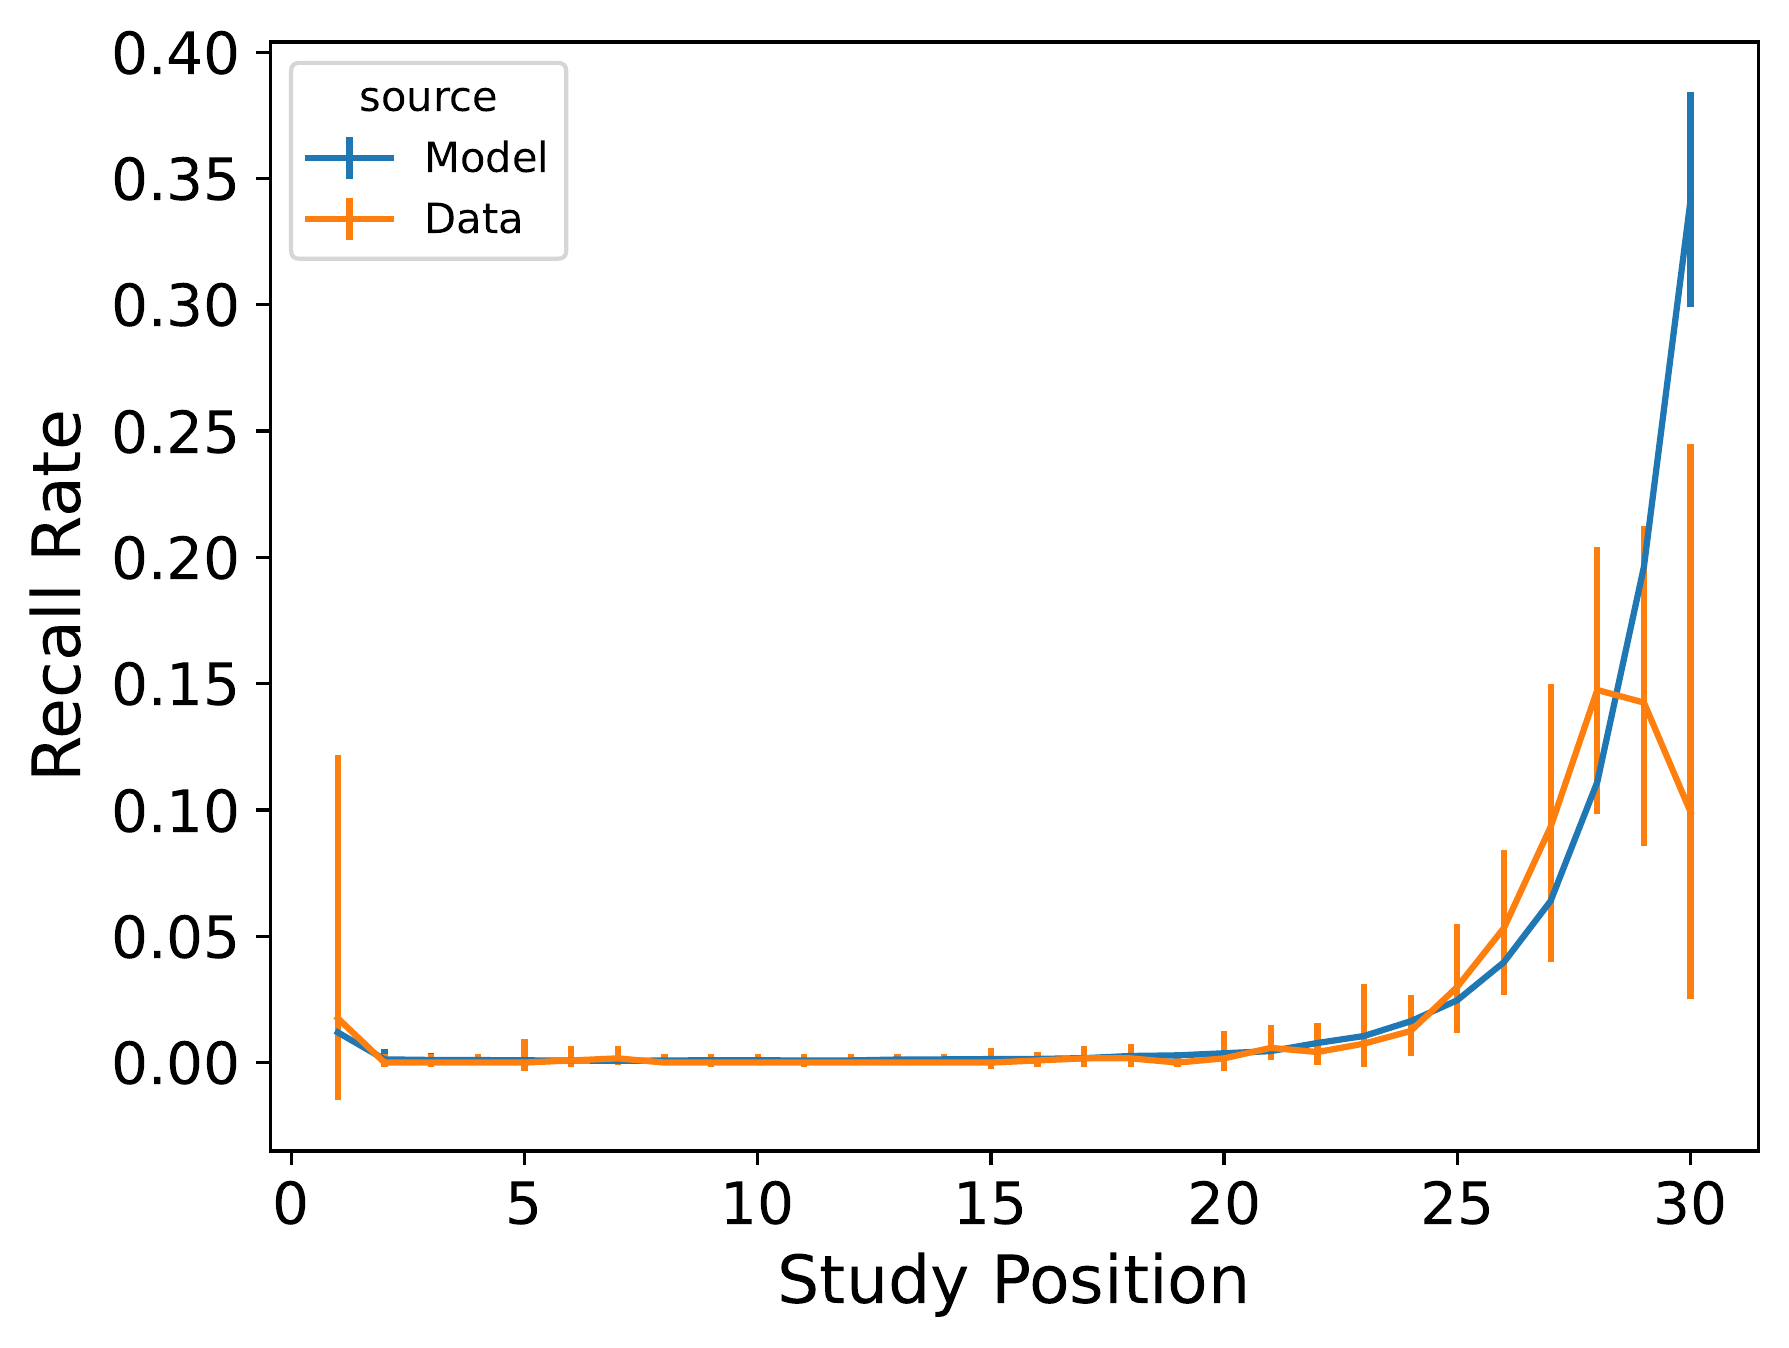
\includegraphics{icmr_figures/Murdock1962_ConnectionistCMR_Model_Fitting_LL30_pnr-1.png}\end{minipage}%
%
\begin{minipage}{0.33\linewidth}
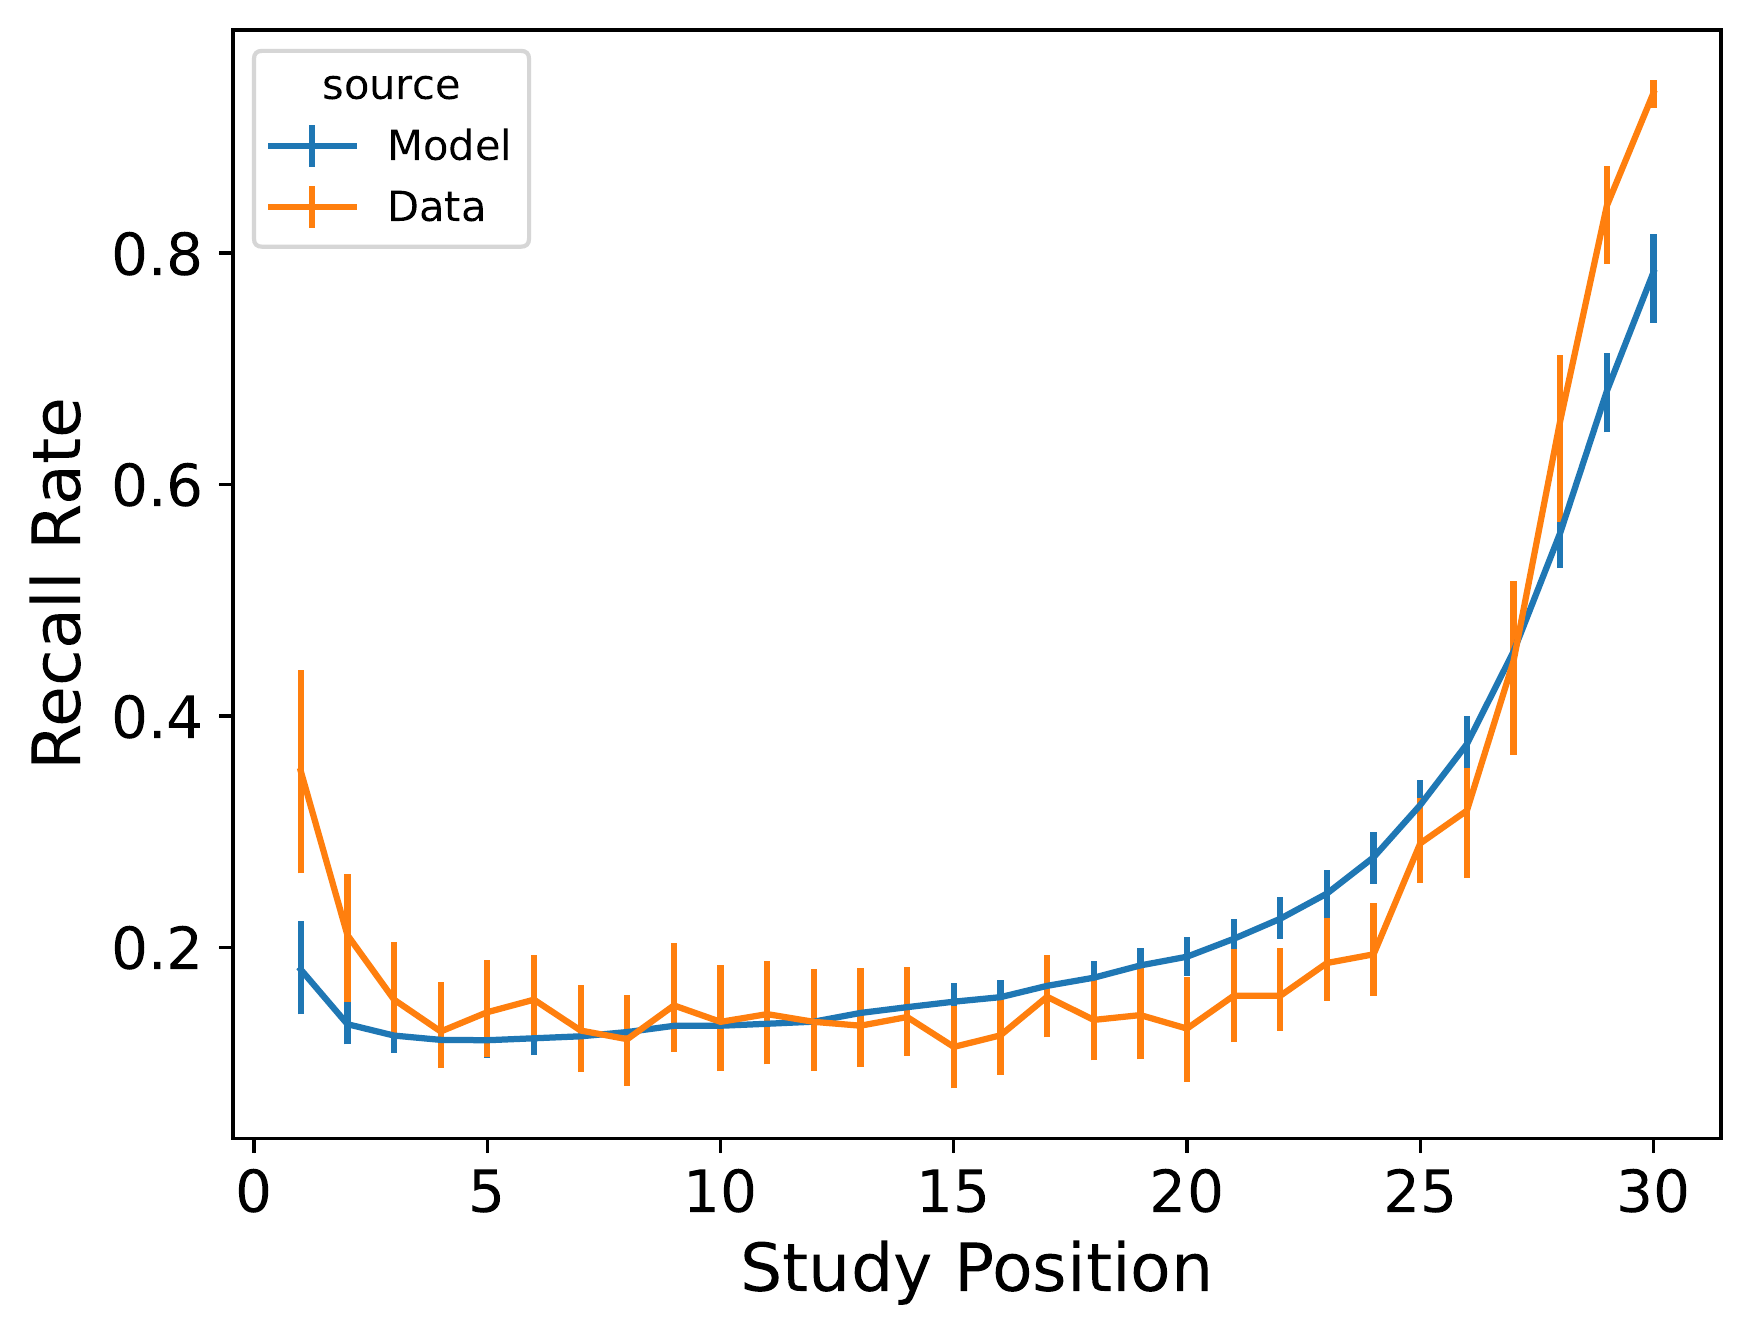
\includegraphics{icmr_figures/Murdock1962_ConnectionistCMR_Model_Fitting_LL30_spc-1.png}\end{minipage}%
\newline
\begin{minipage}{0.33\linewidth}
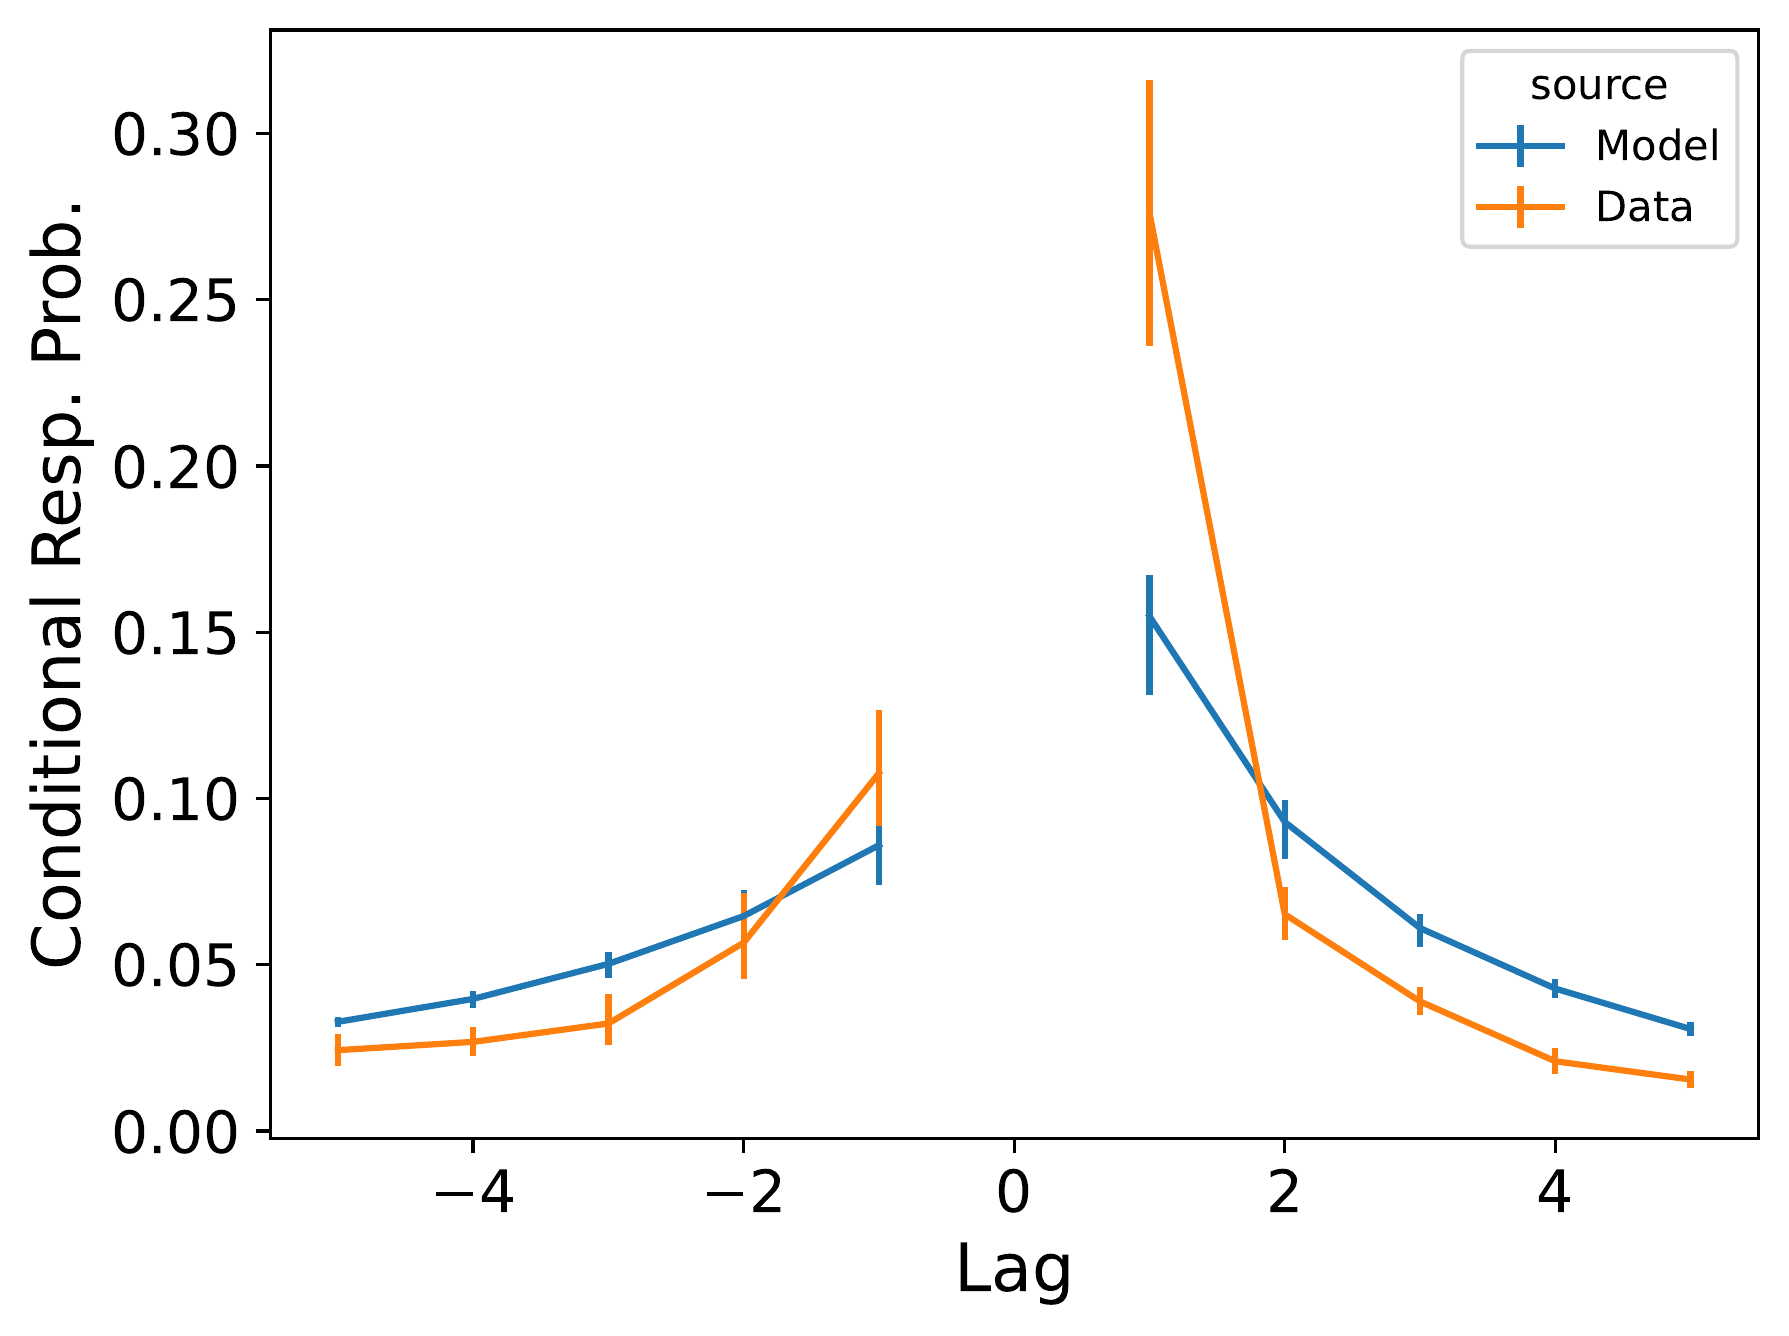
\includegraphics{icmr_figures/Murdock1962_InstanceCMR_Model_Fitting_LL30_crp-1.png}\end{minipage}%
%
\begin{minipage}{0.33\linewidth}
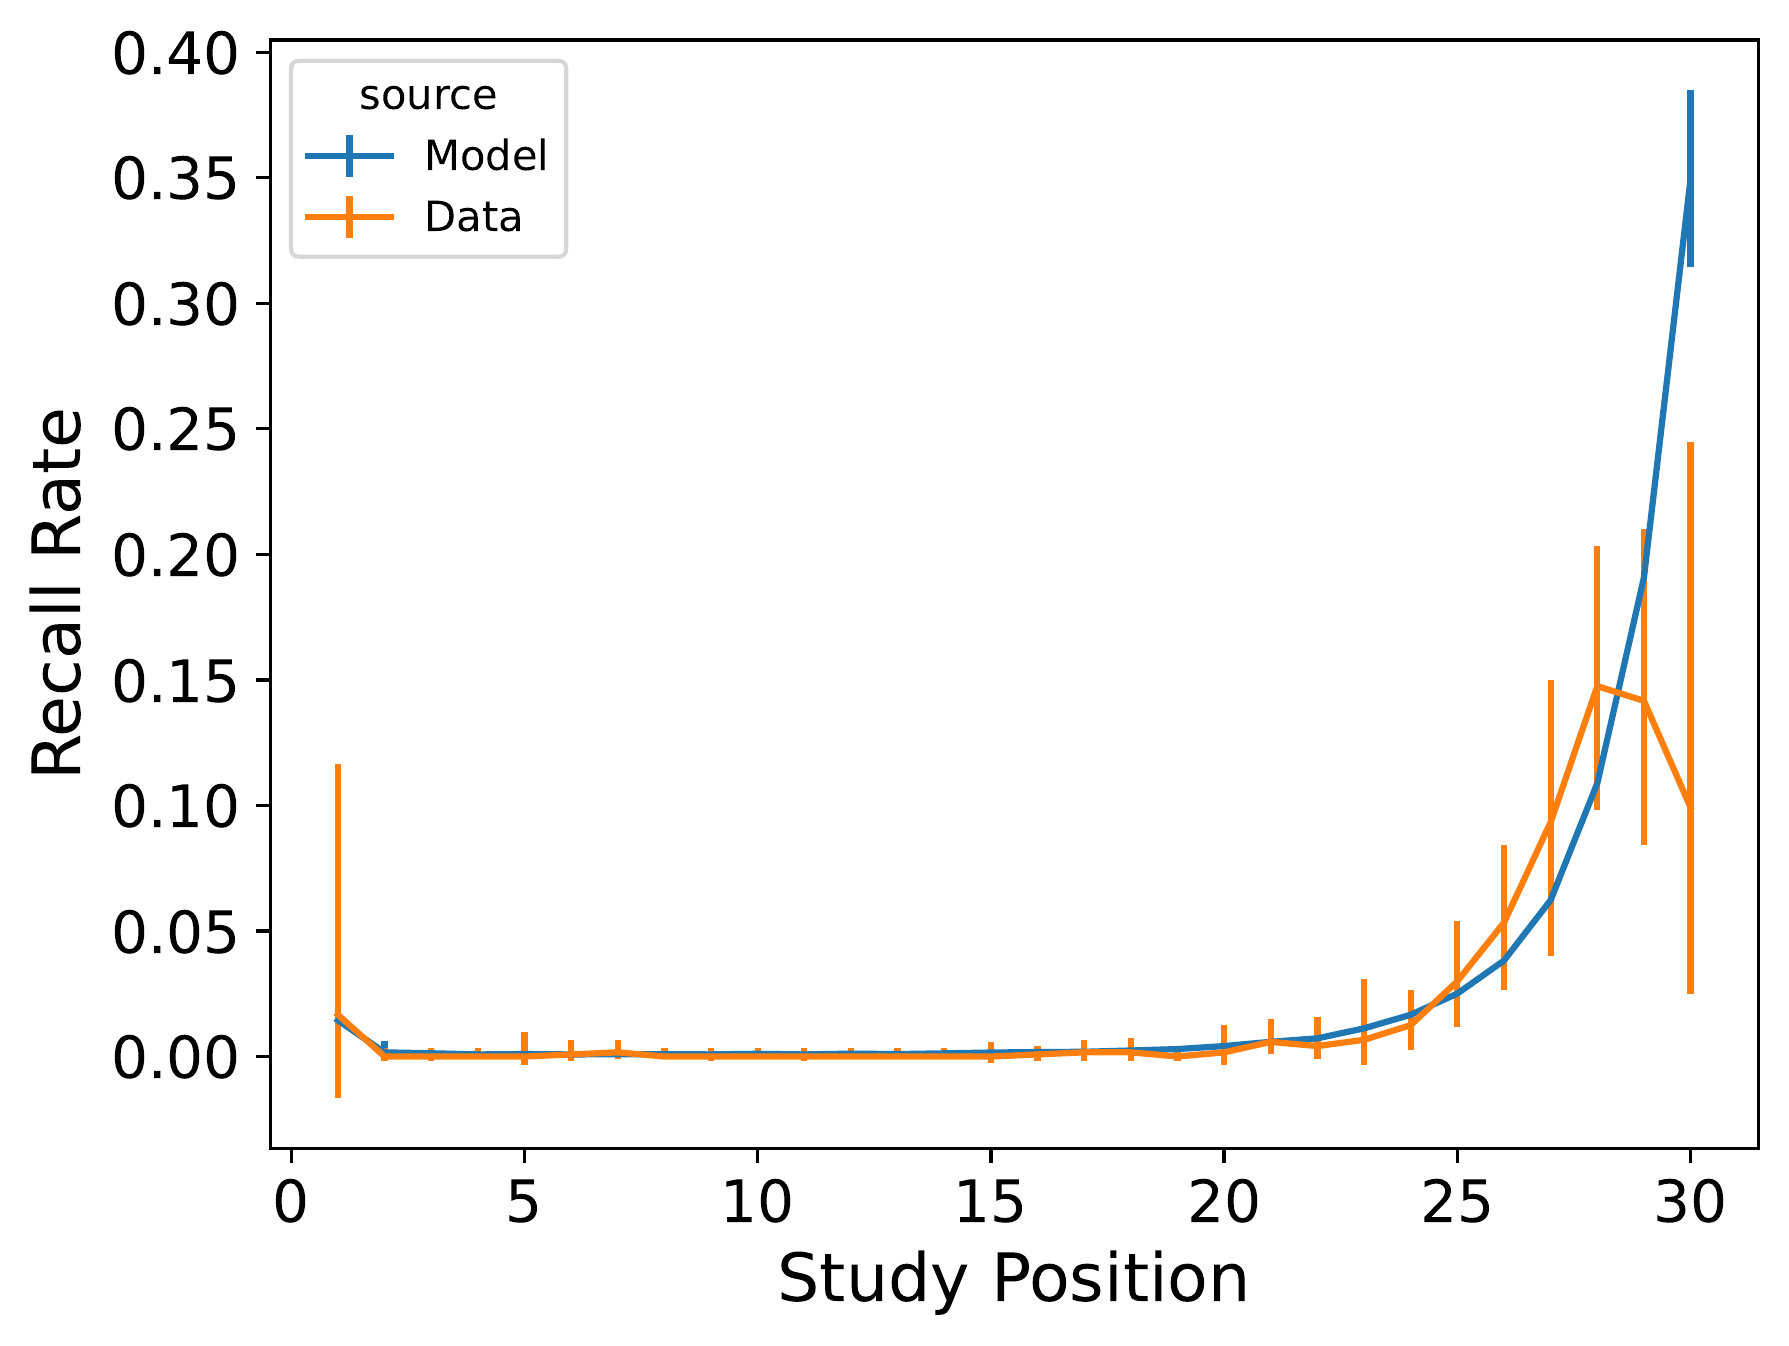
\includegraphics{icmr_figures/Murdock1962_InstanceCMR_Model_Fitting_LL30_pnr-1.png}\end{minipage}%
%
\begin{minipage}{0.33\linewidth}
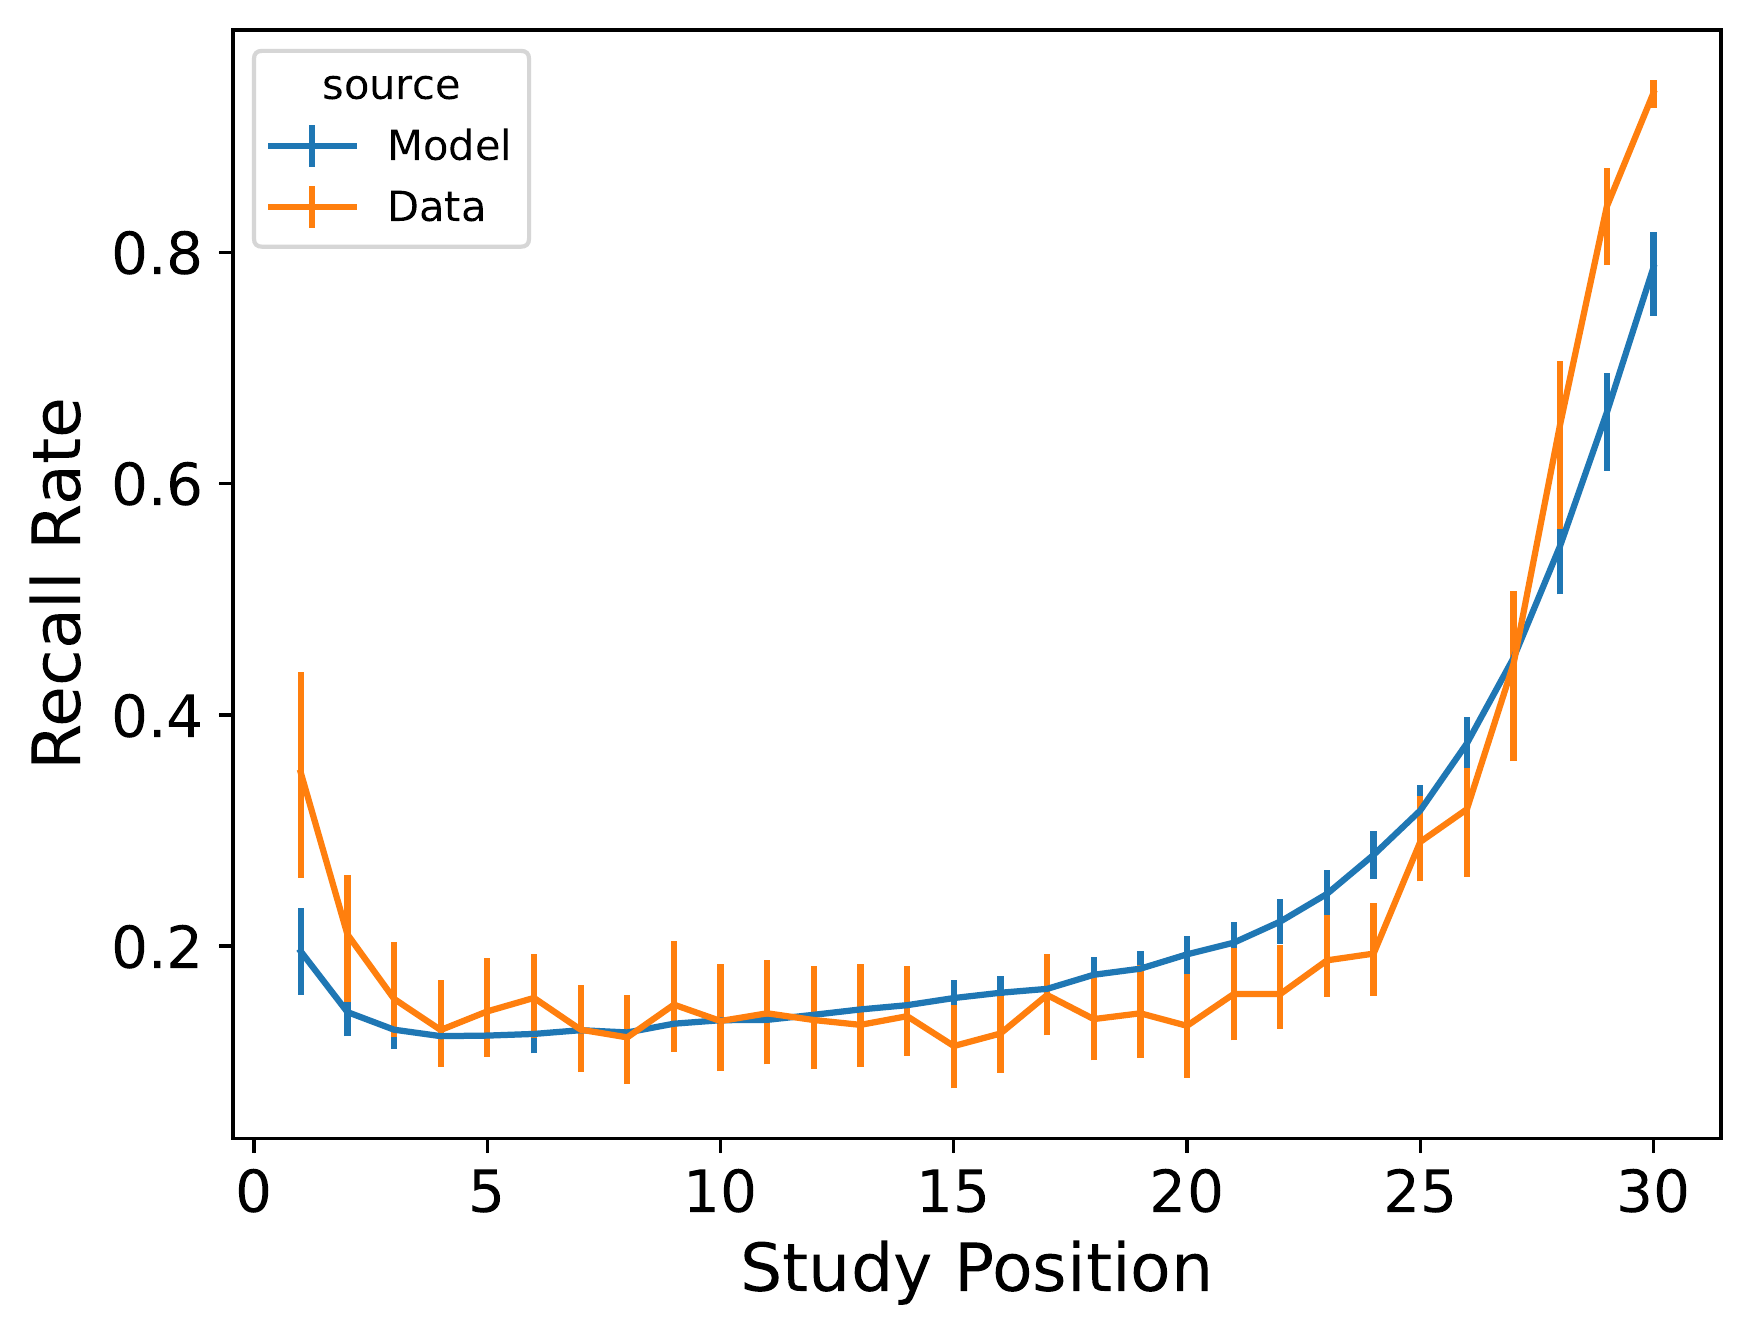
\includegraphics{icmr_figures/Murdock1962_InstanceCMR_Model_Fitting_LL30_spc-1.png}\end{minipage}%
\newline
\begin{minipage}{0.33\linewidth}
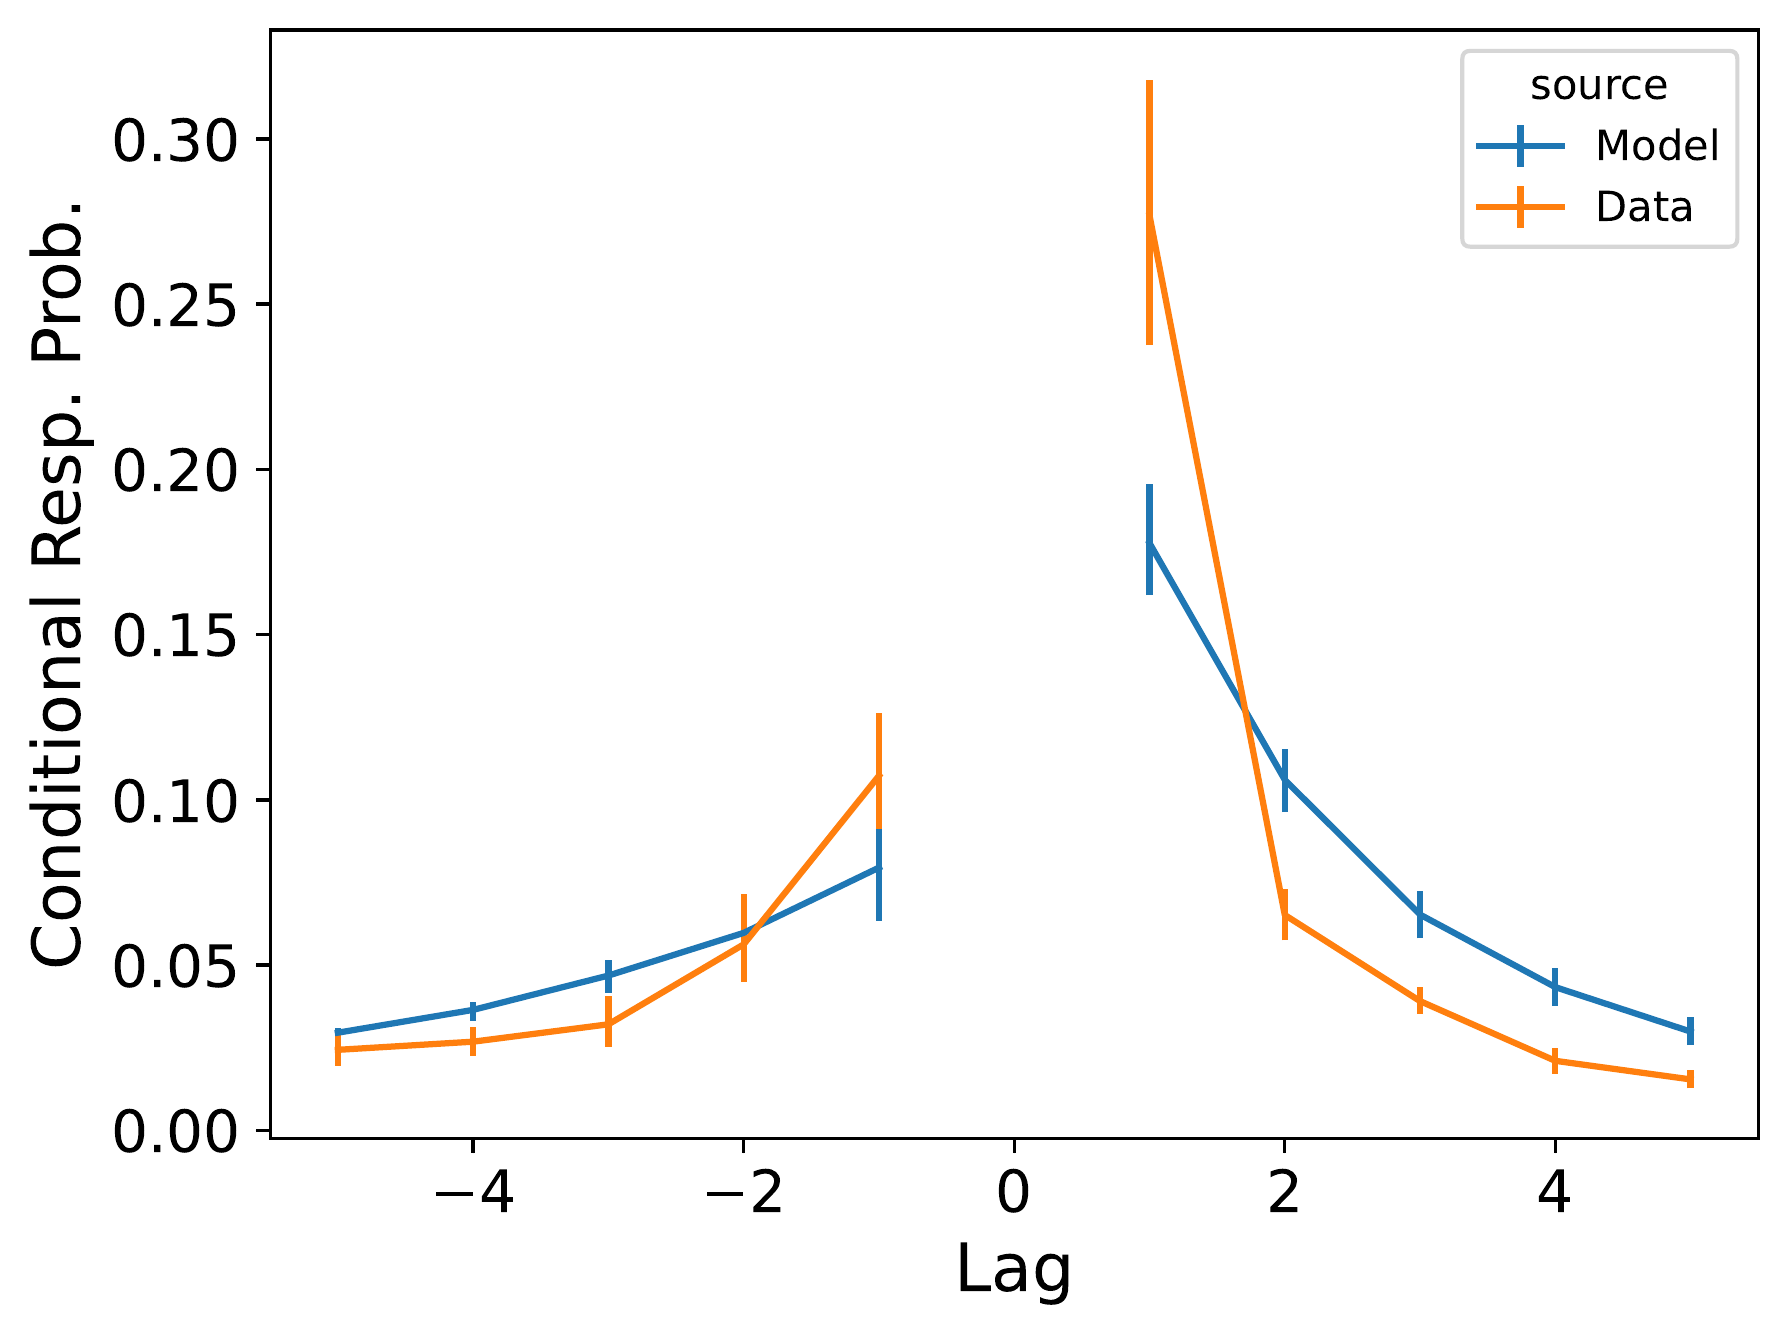
\includegraphics{icmr_figures/Murdock1962_TraceScalingCMR_Model_Fitting_LL30_crp-1.png}\end{minipage}%
%
\begin{minipage}{0.33\linewidth}
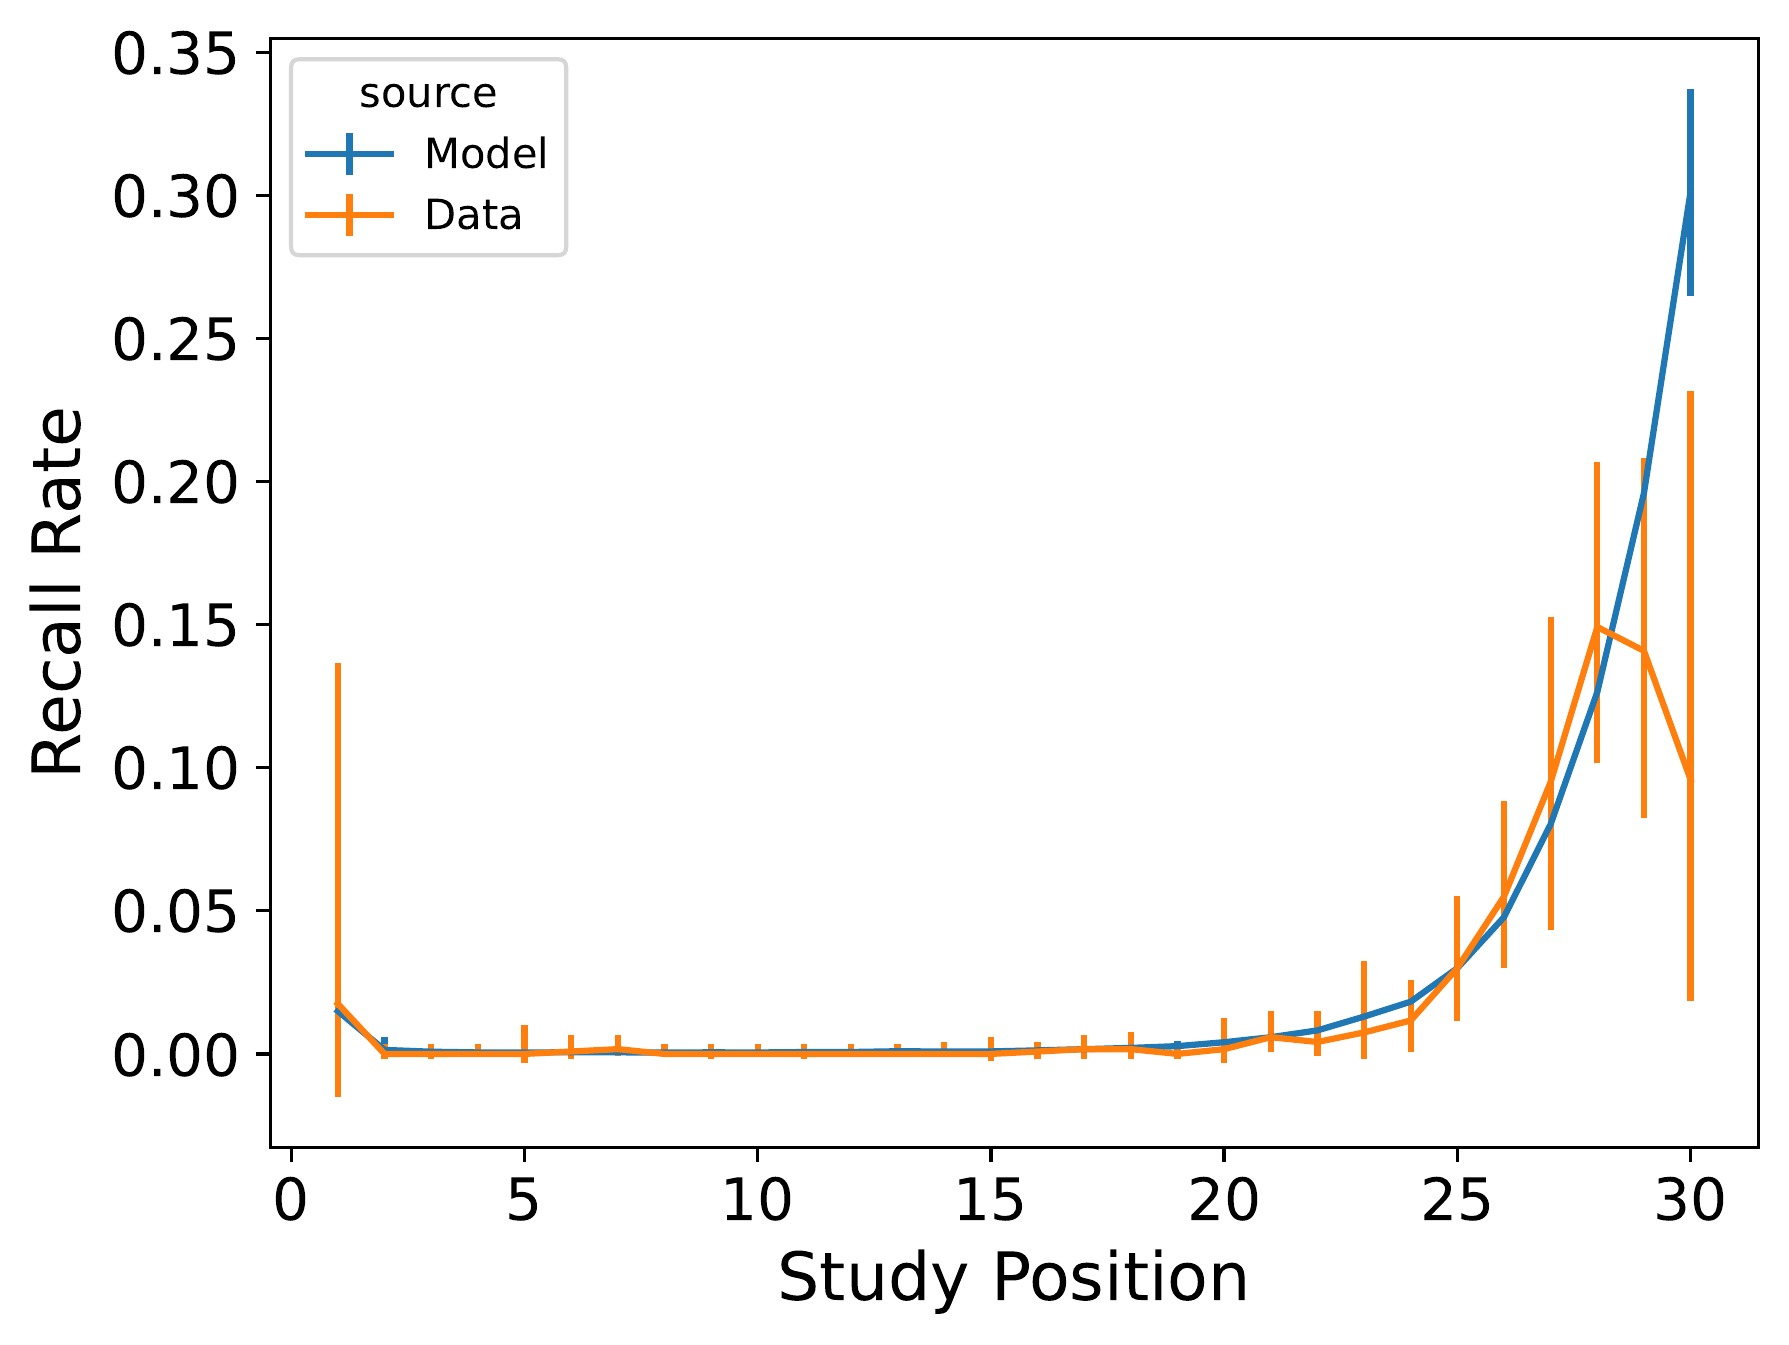
\includegraphics{icmr_figures/Murdock1962_TraceScalingCMR_Model_Fitting_LL30_pnr-1.png}\end{minipage}%
%
\begin{minipage}{0.33\linewidth}
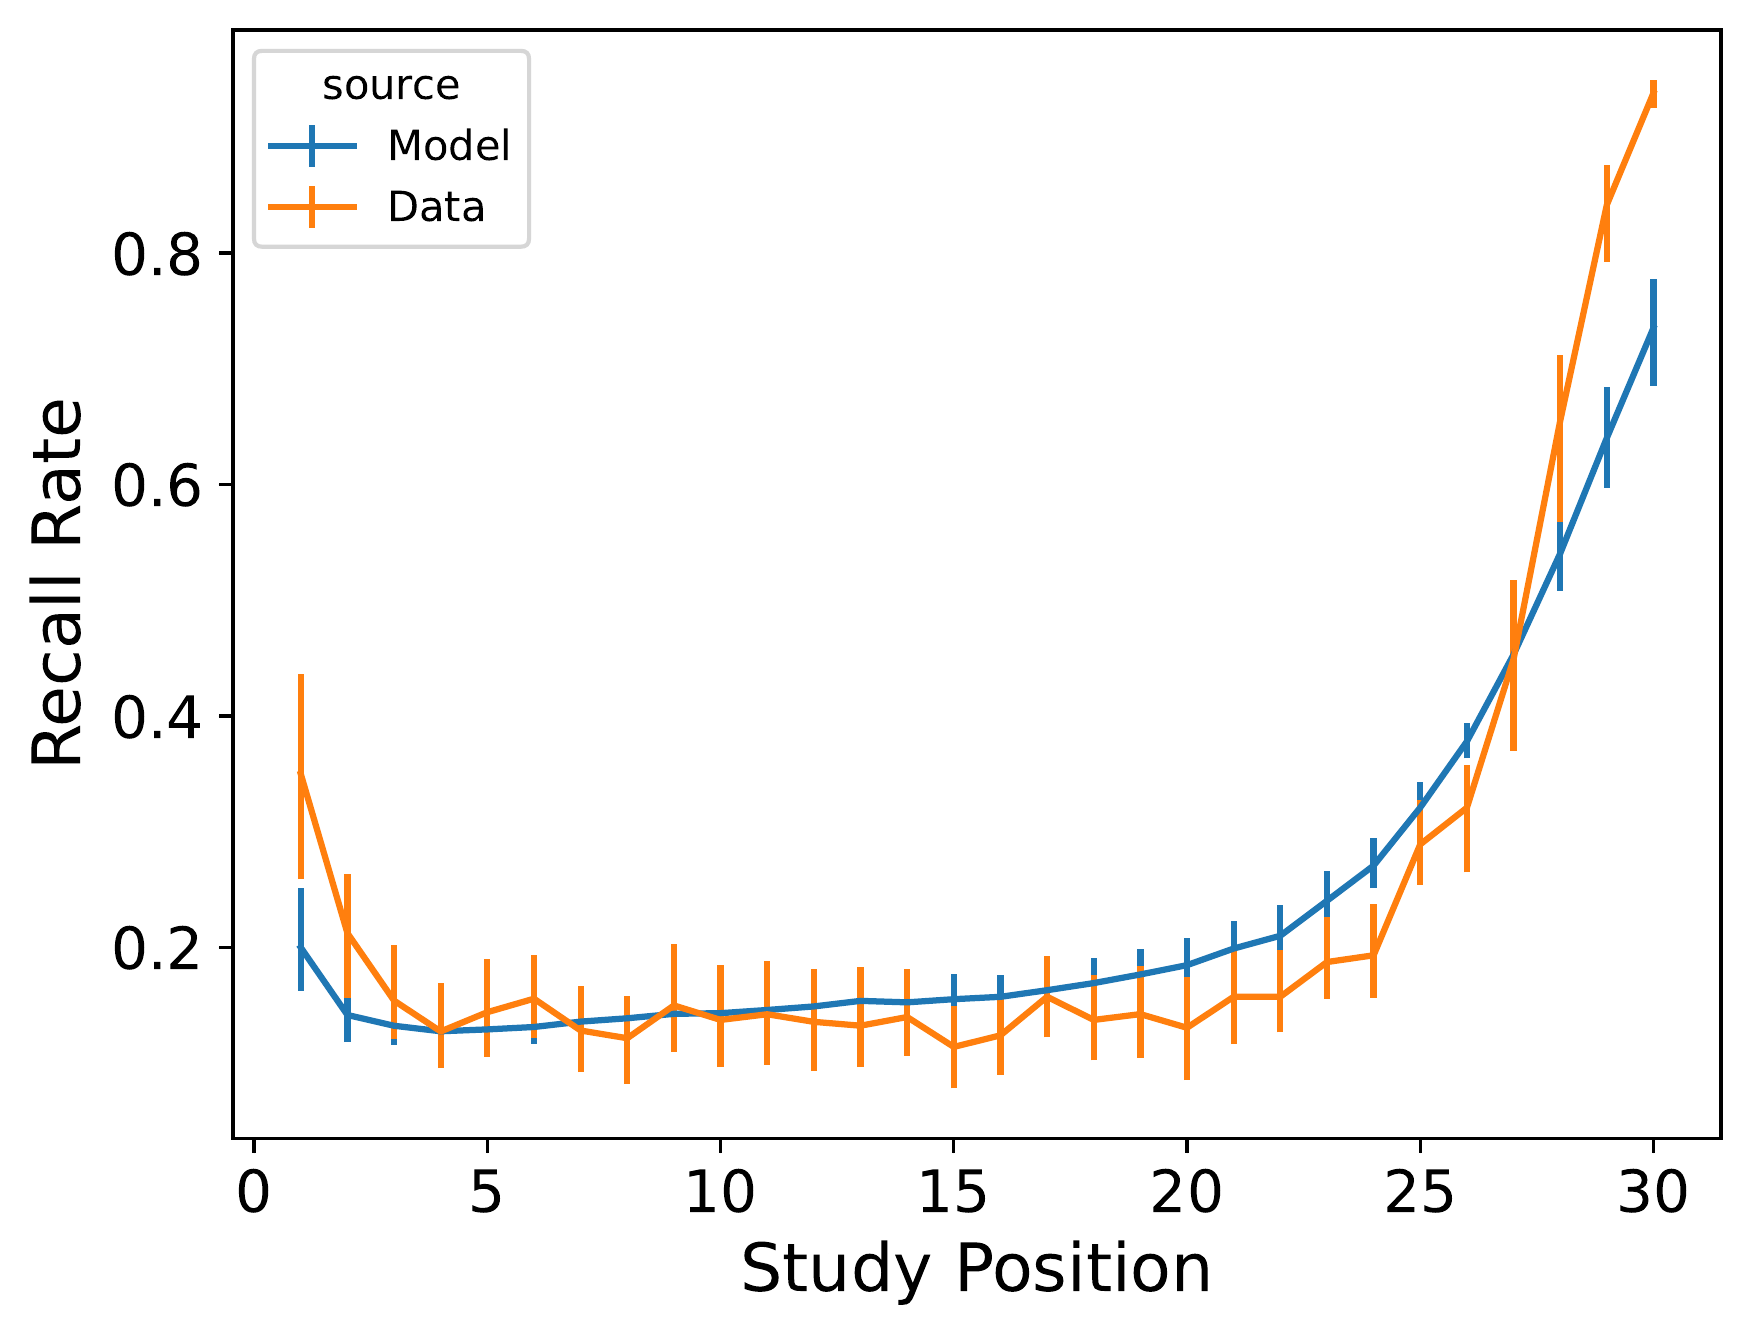
\includegraphics{icmr_figures/Murdock1962_TraceScalingCMR_Model_Fitting_LL30_spc-1.png}\end{minipage}%
\newline
\begin{minipage}{0.33\linewidth}
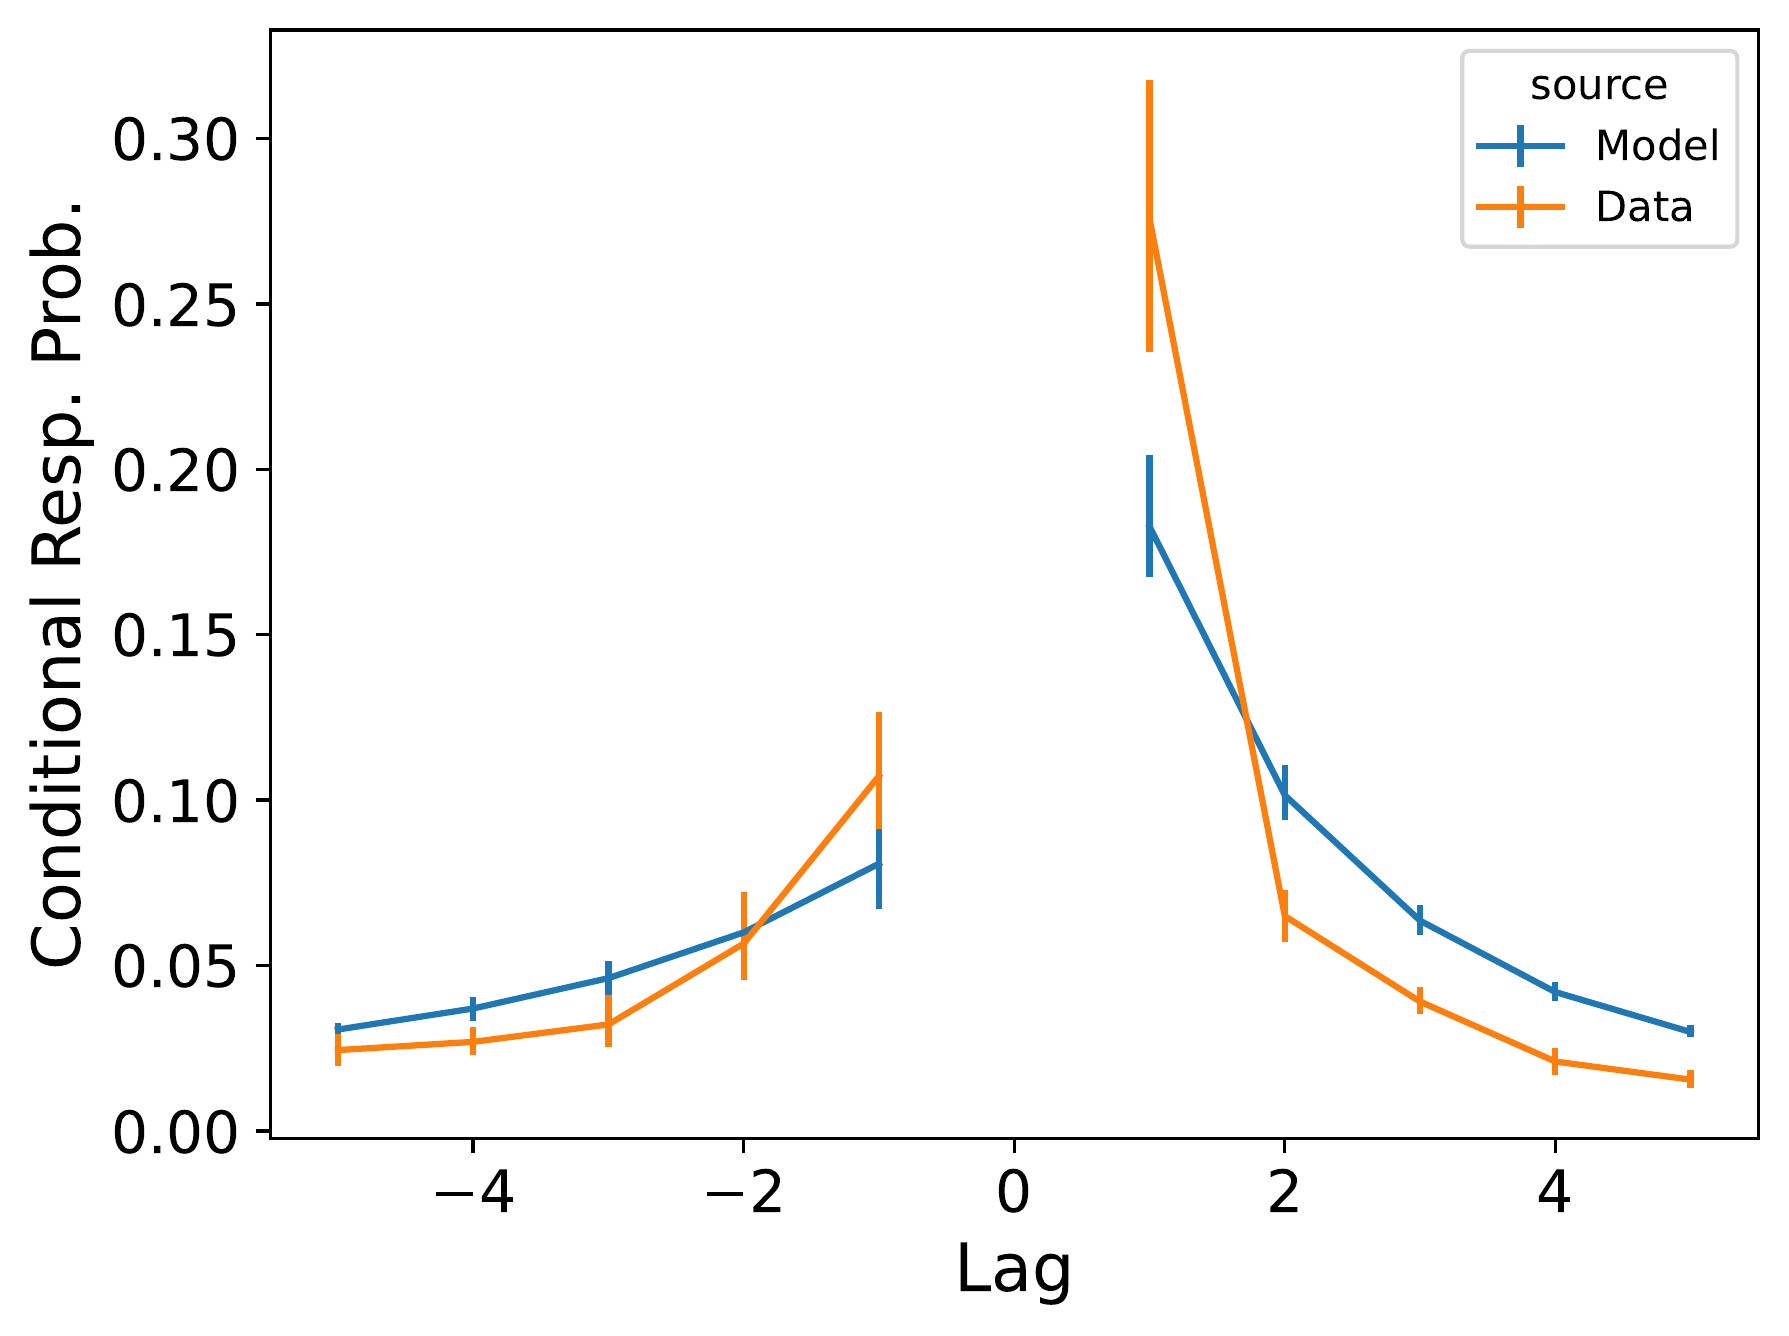
\includegraphics{icmr_figures/Murdock1962_MultiScalingCMR_Model_Fitting_LL30_crp-1.png}\end{minipage}%
%
\begin{minipage}{0.33\linewidth}
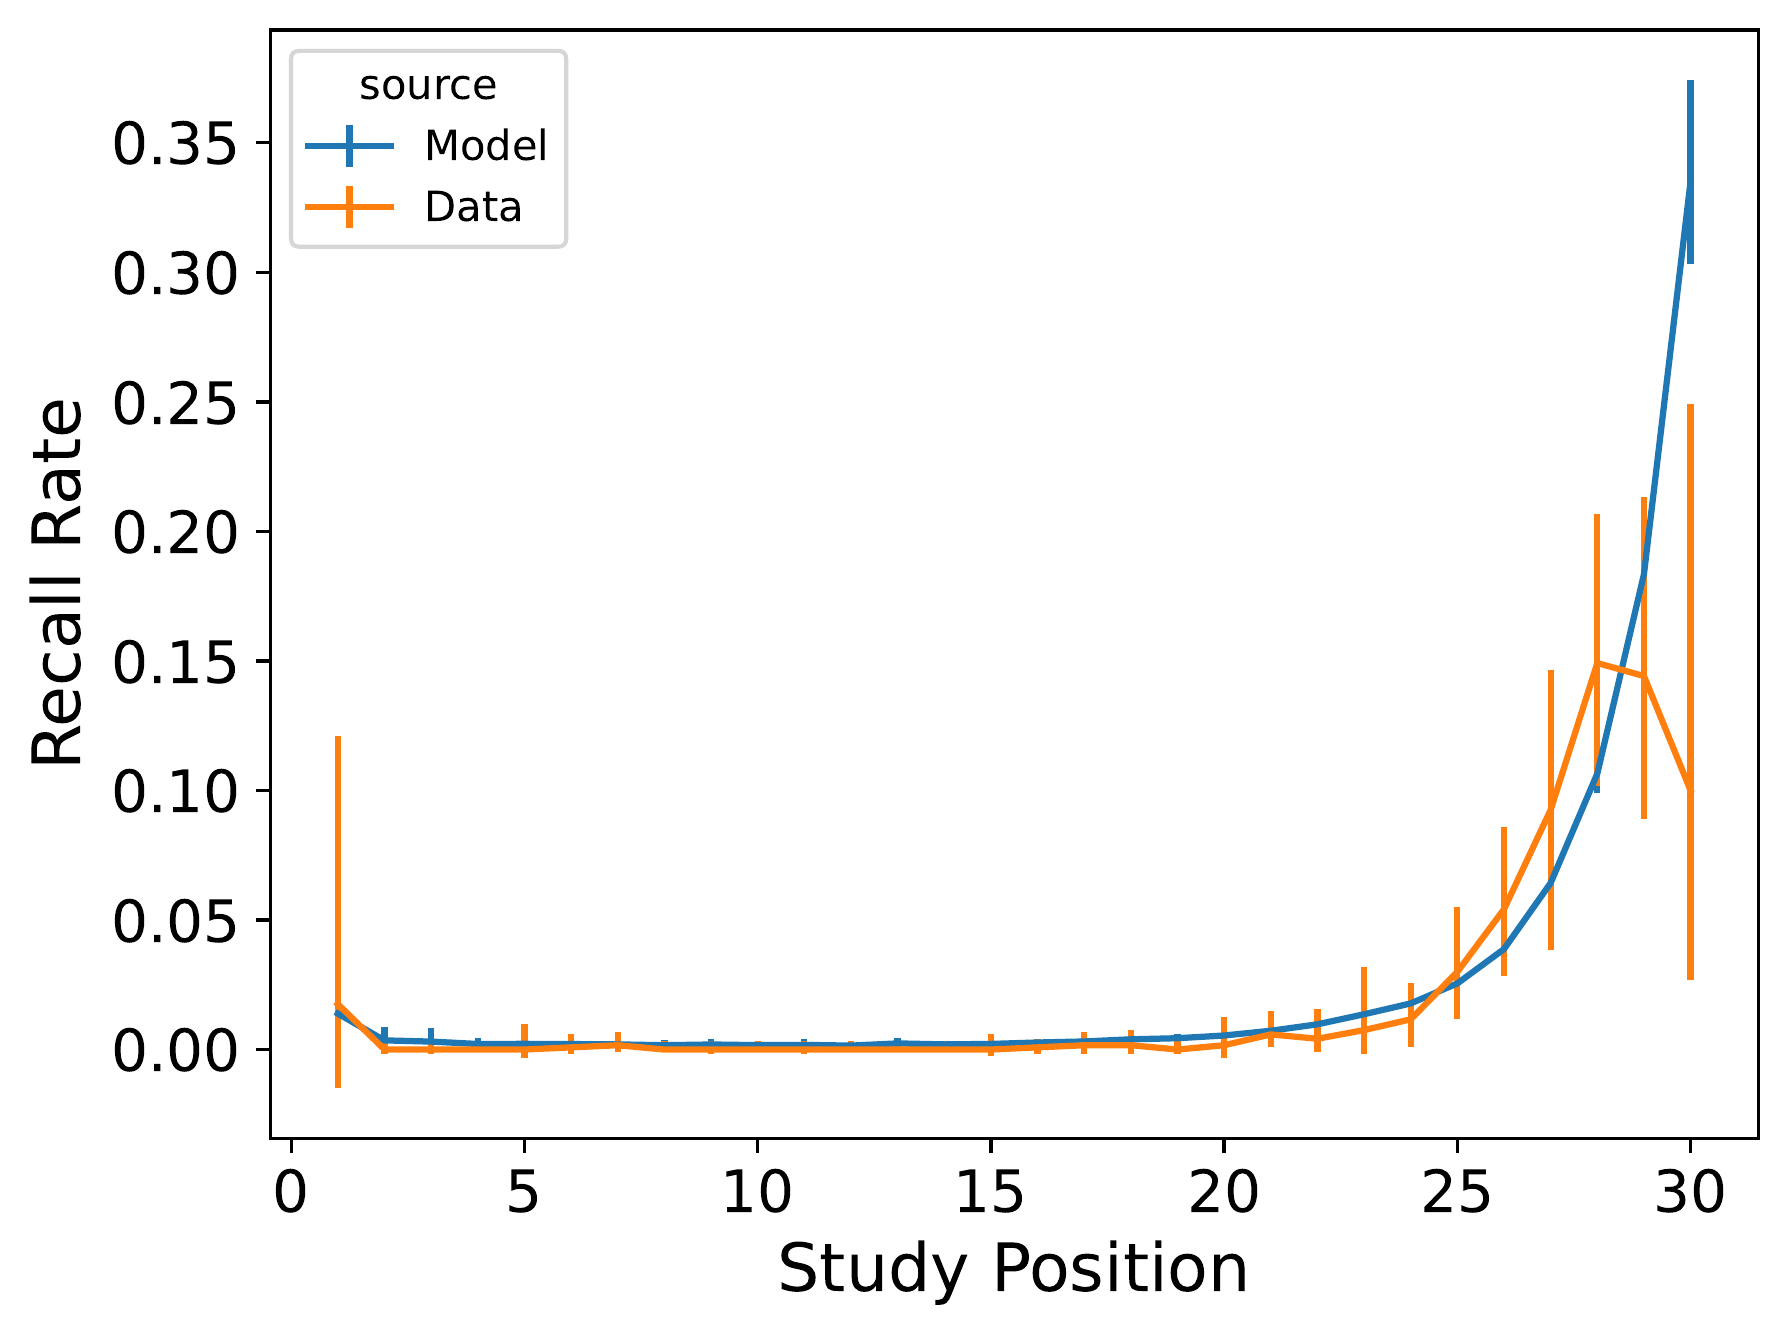
\includegraphics{icmr_figures/Murdock1962_MultiScalingCMR_Model_Fitting_LL30_pnr-1.png}\end{minipage}%
%
\begin{minipage}{0.33\linewidth}
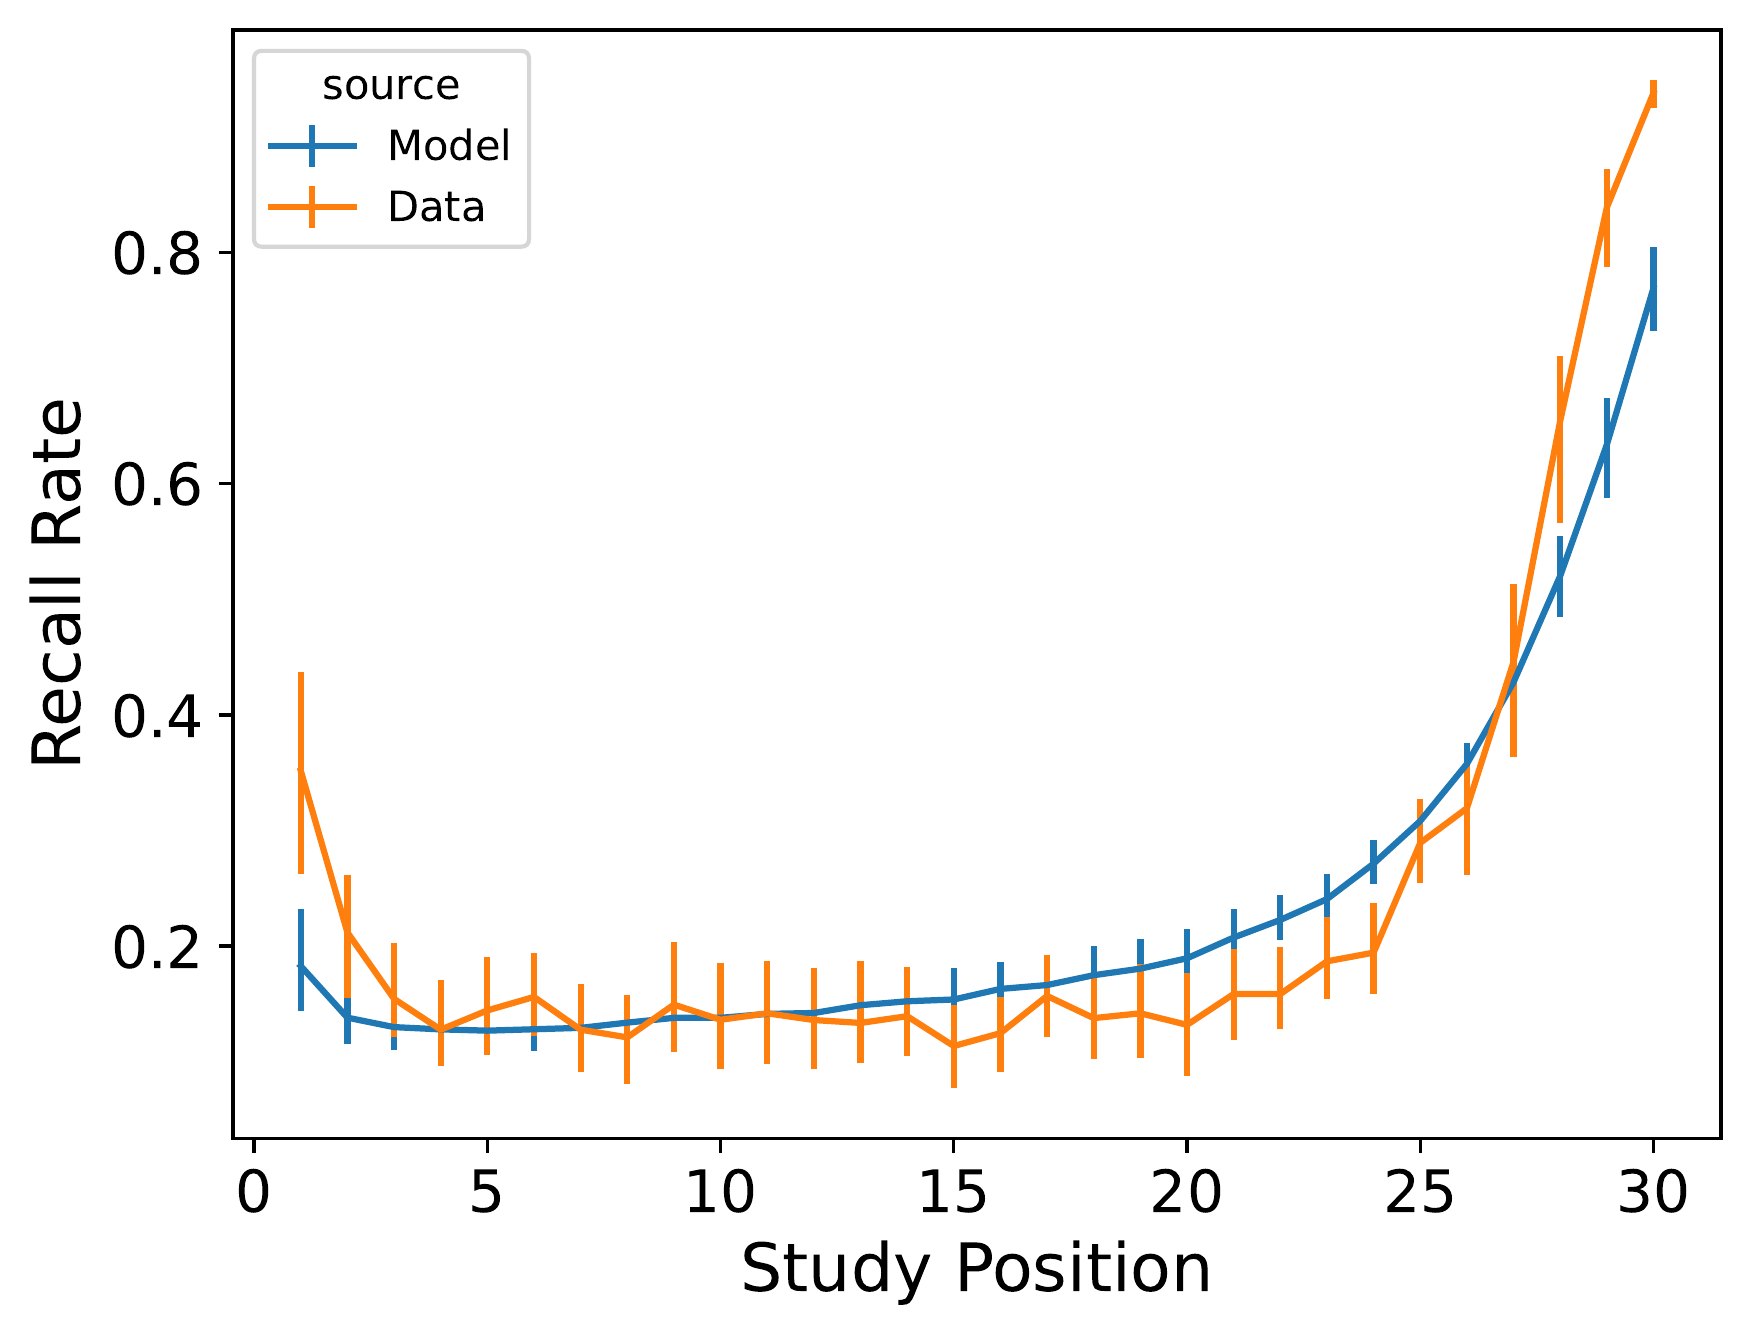
\includegraphics{icmr_figures/Murdock1962_MultiScalingCMR_Model_Fitting_LL30_spc-1.png}\end{minipage}%

\caption{\label{fig-murdock1962memory30}Summary statistic fits to
Murdock Jr (1962) where list length = 30. Top: Connectionist CMR. Second
Row: Instance CMR, \(\tau_{t}\) set to 1. Third Row: Trace Scaling CMR
-- Instance CMR, \(\tau_{c}\) set to 1 and \(\tau_{t}\) optimized during
fitting. Fourth Row: Multi Scaling CMR -- Instance CMR, both \(\tau_t\)
and \(\tau_c\) freed for fitting. Left: conditional response probability
as a function of lag. Middle: probability of starting recall with each
serial position. Right: recall probability as a function of serial
position.}

\end{figure}%

\begin{figure}

\begin{minipage}{0.33\linewidth}
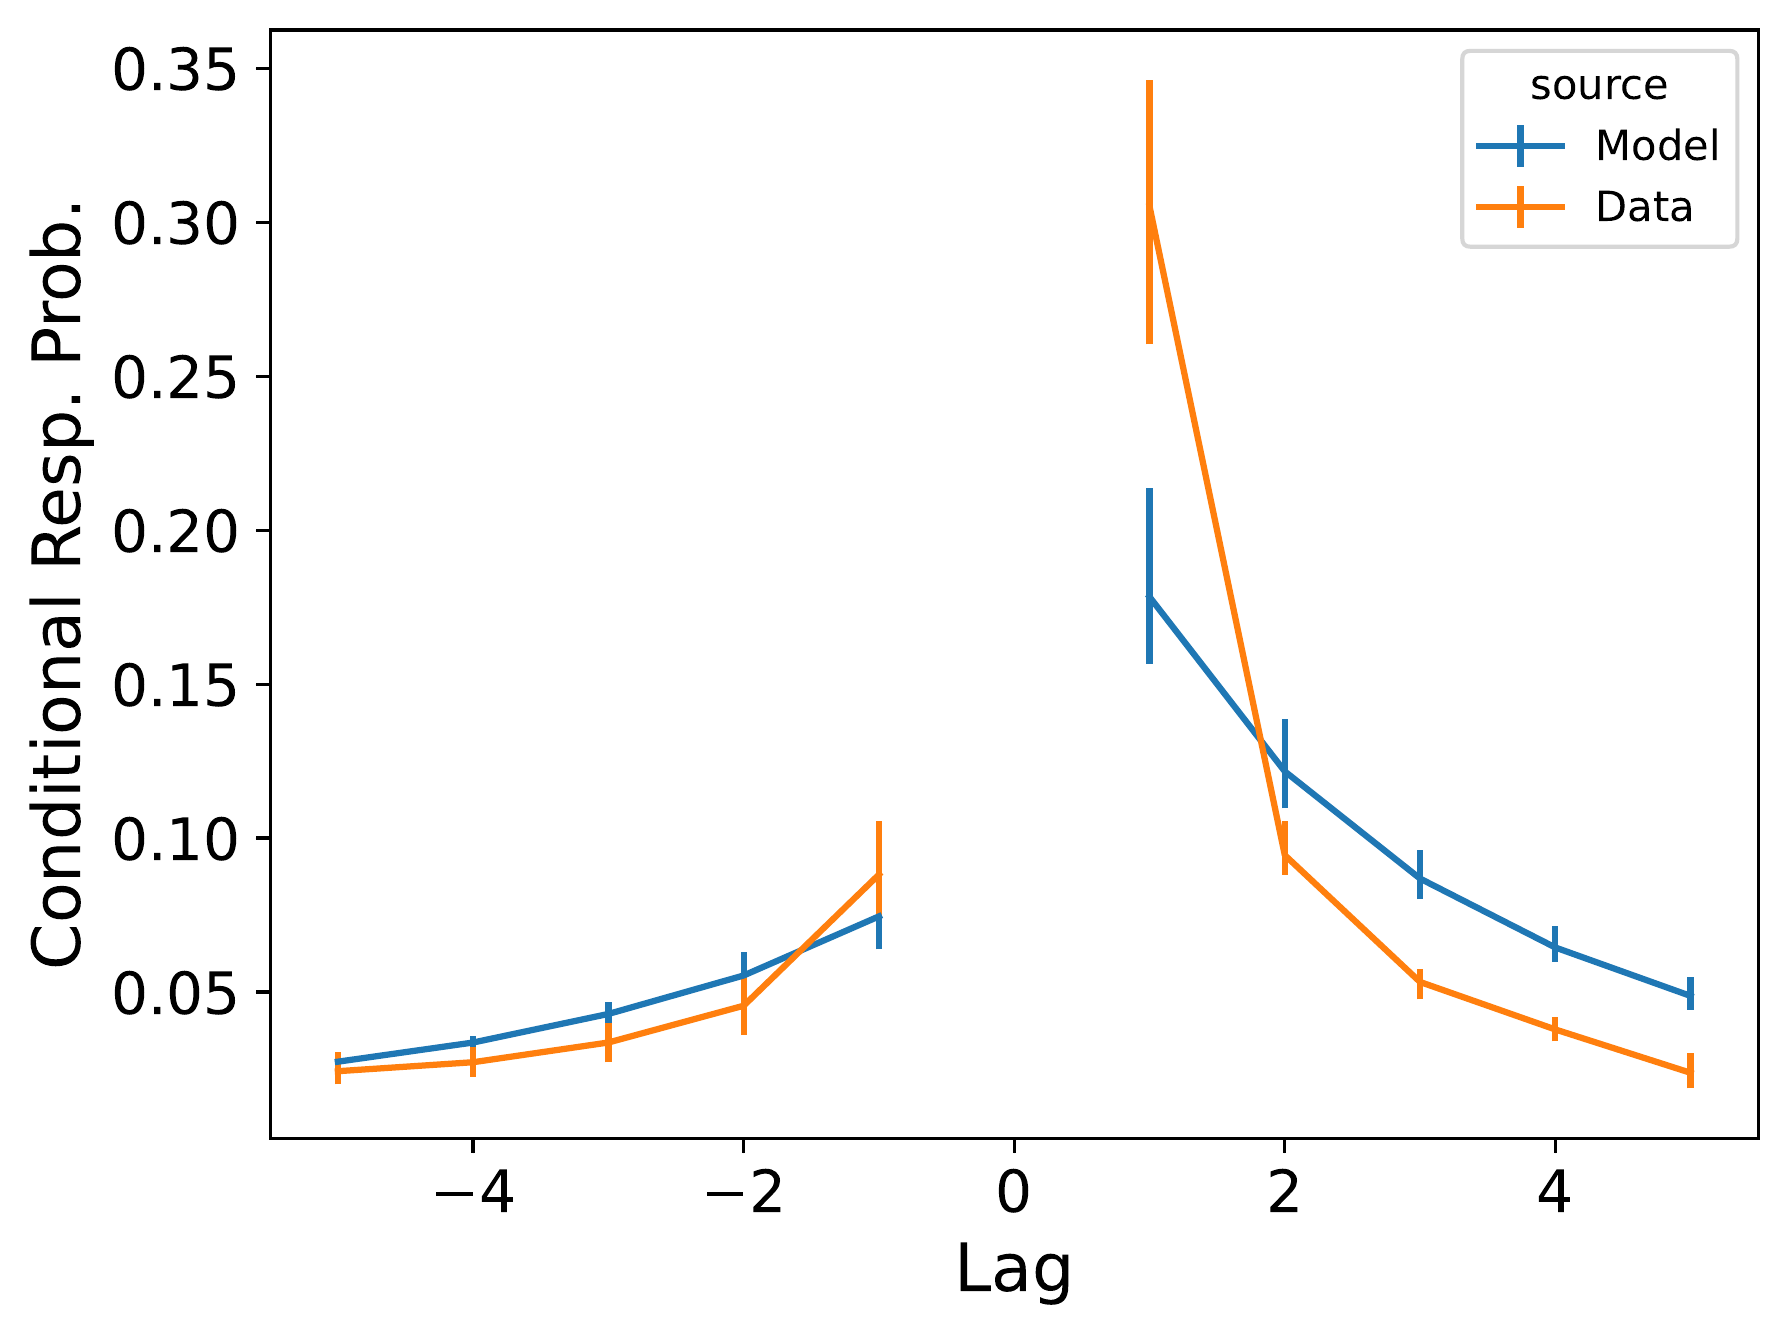
\includegraphics{icmr_figures/Murdock1962_ConnectionistCMR_Model_Fitting_LL40_crp-1.png}\end{minipage}%
%
\begin{minipage}{0.33\linewidth}
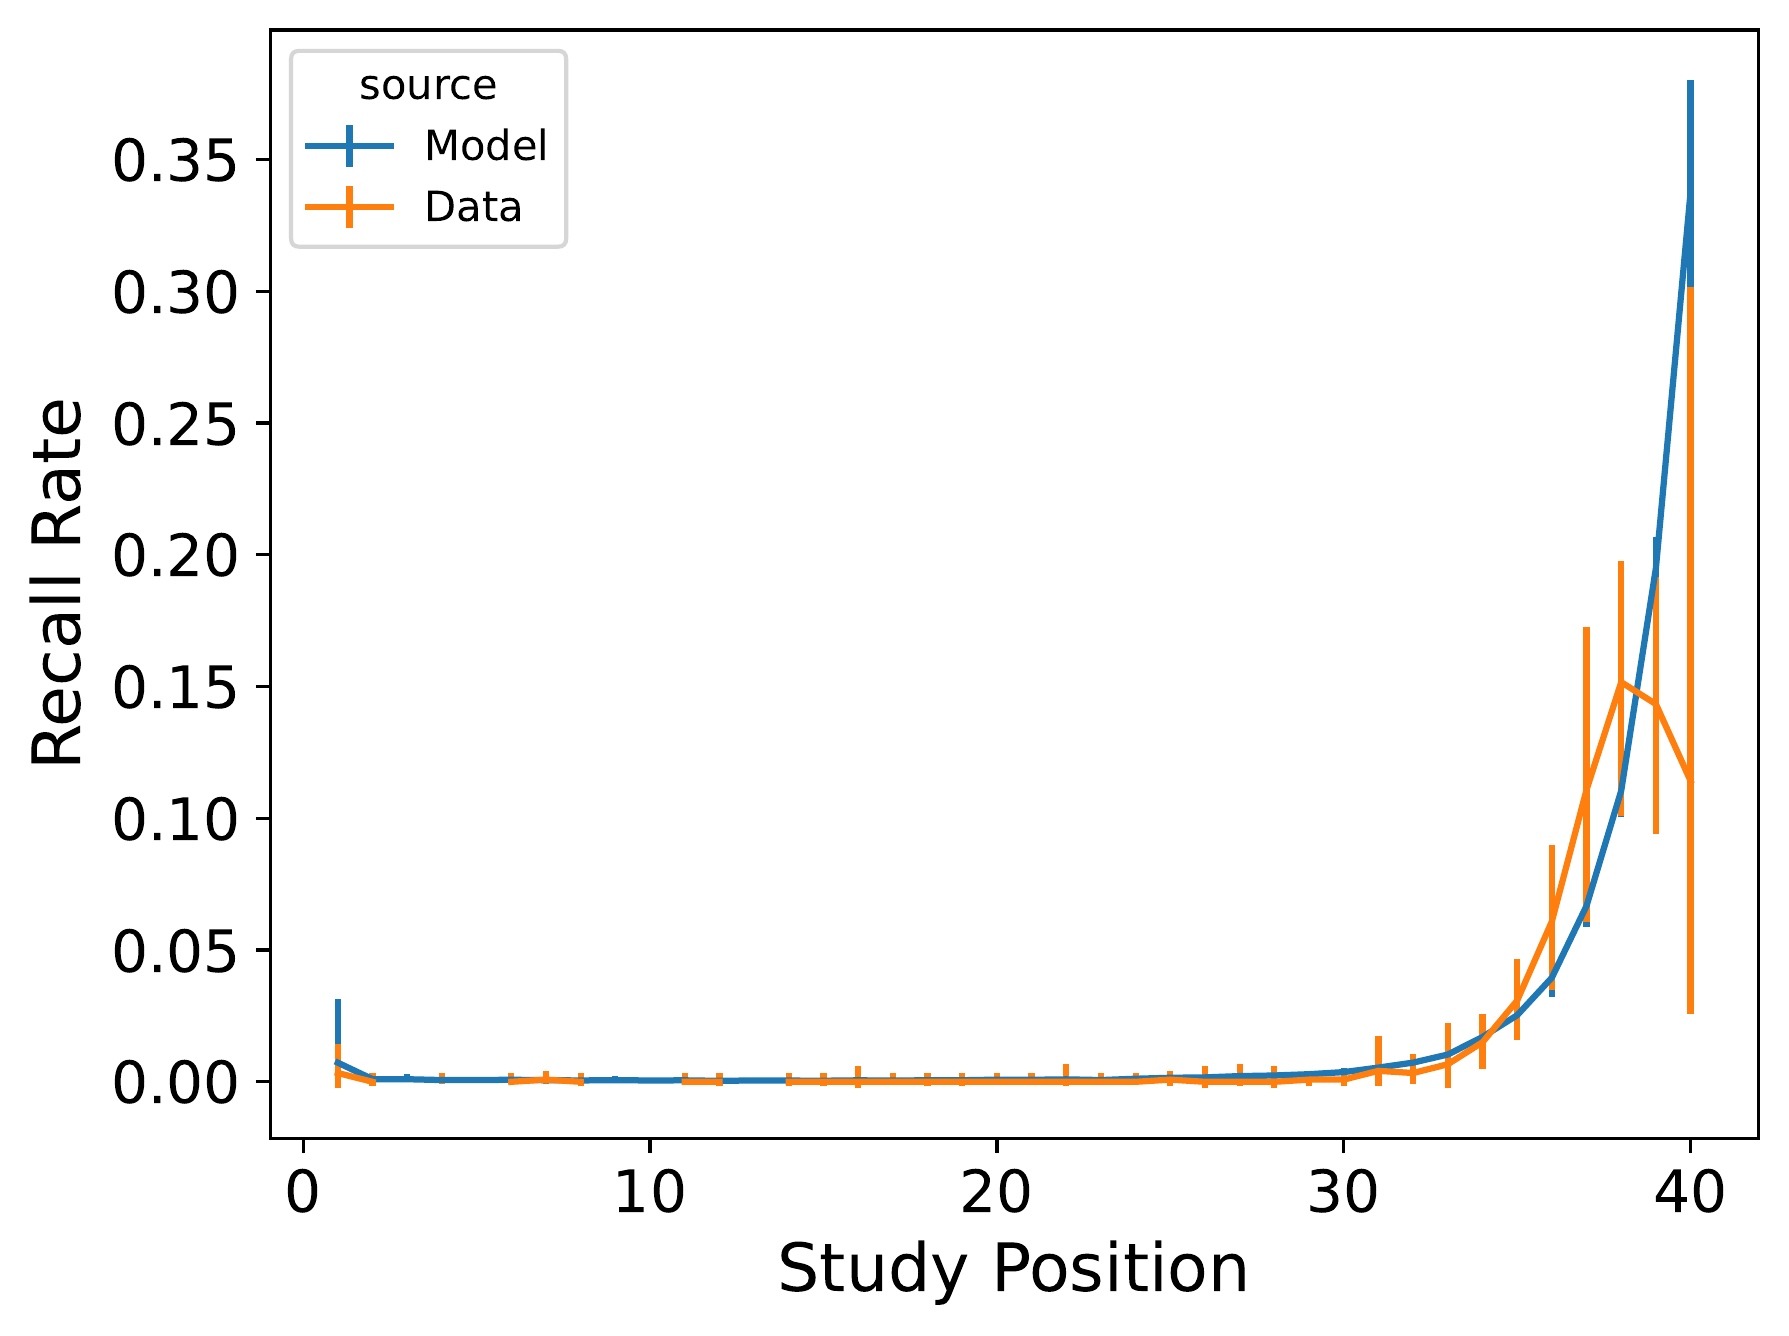
\includegraphics{icmr_figures/Murdock1962_ConnectionistCMR_Model_Fitting_LL40_pnr-1.png}\end{minipage}%
%
\begin{minipage}{0.33\linewidth}
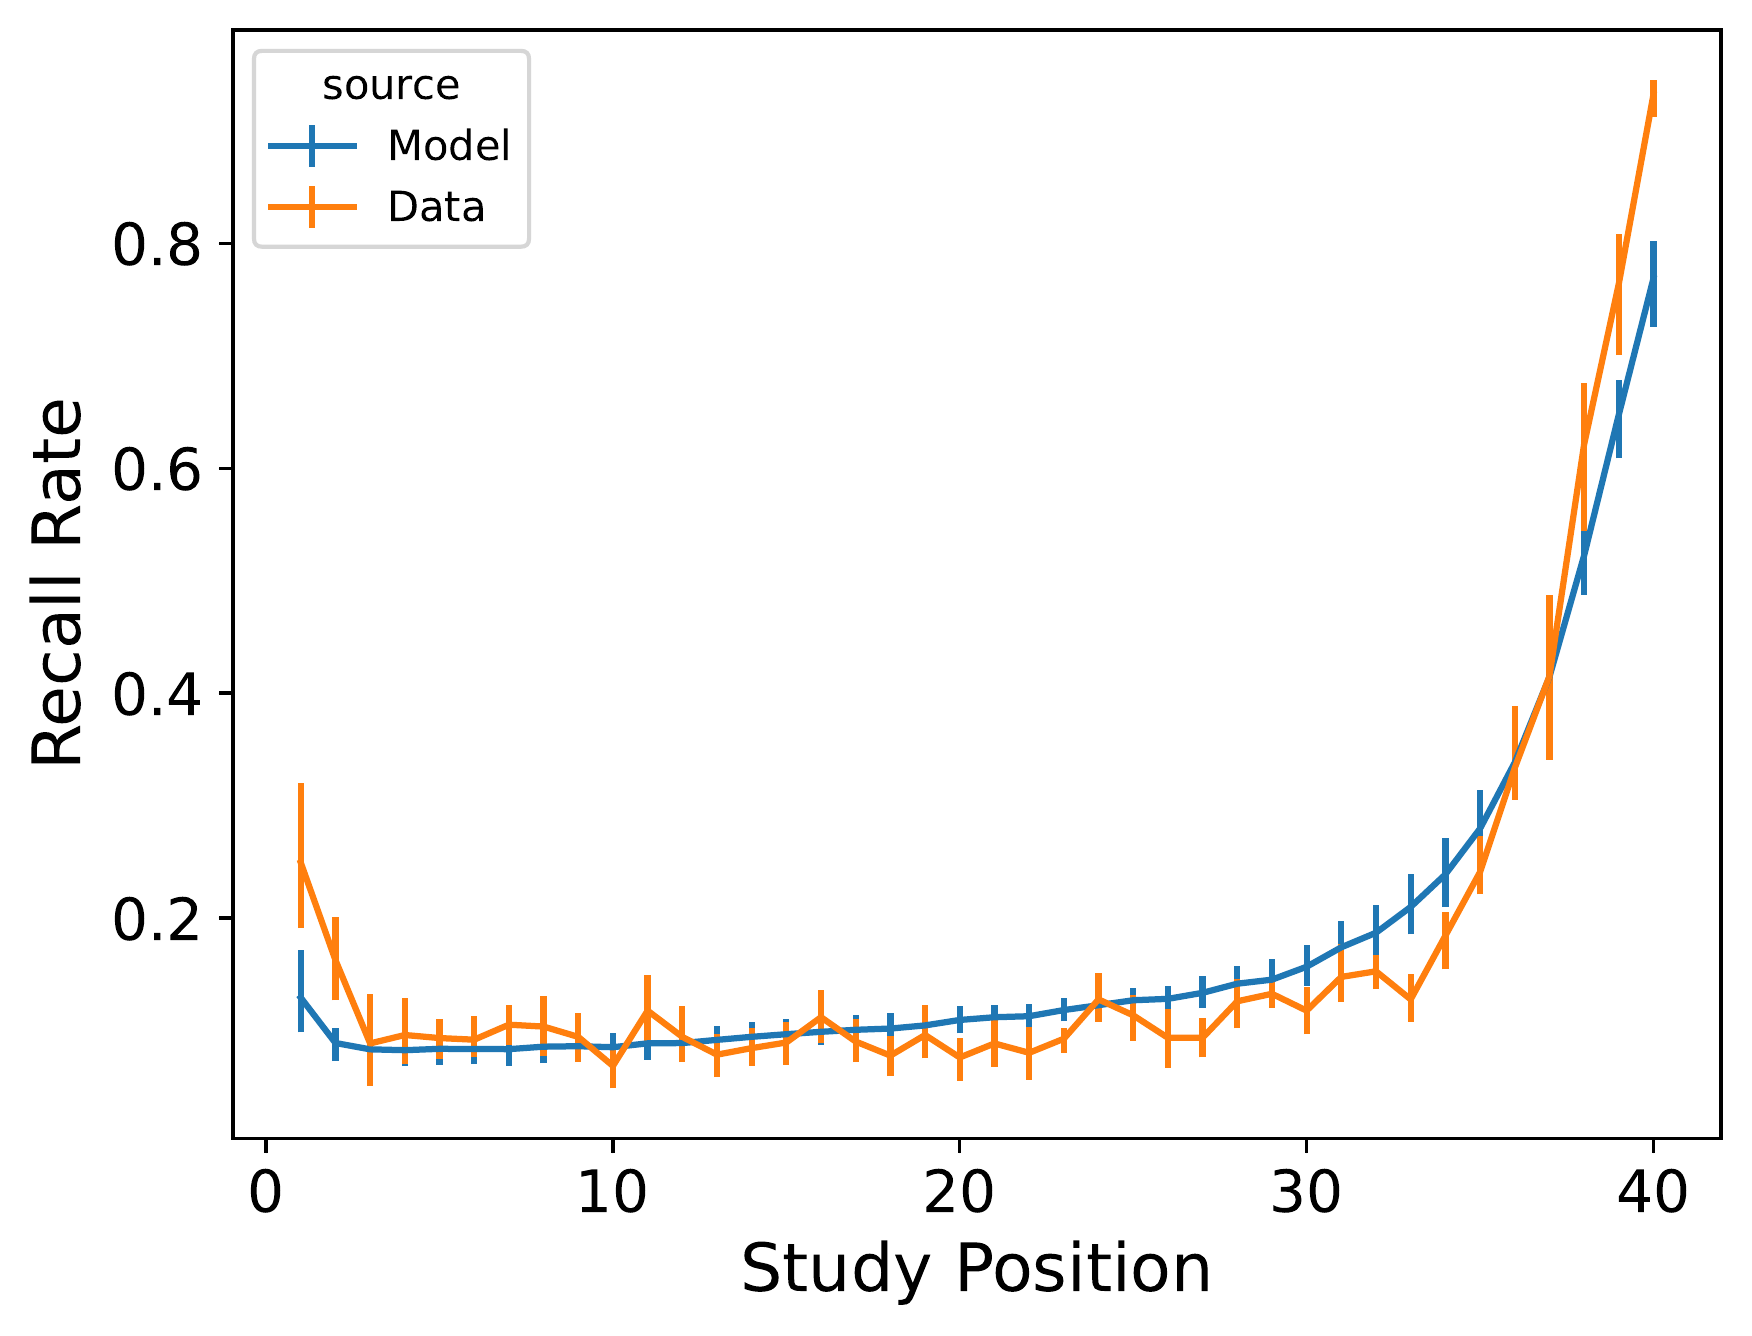
\includegraphics{icmr_figures/Murdock1962_ConnectionistCMR_Model_Fitting_LL40_spc-1.png}\end{minipage}%
\newline
\begin{minipage}{0.33\linewidth}
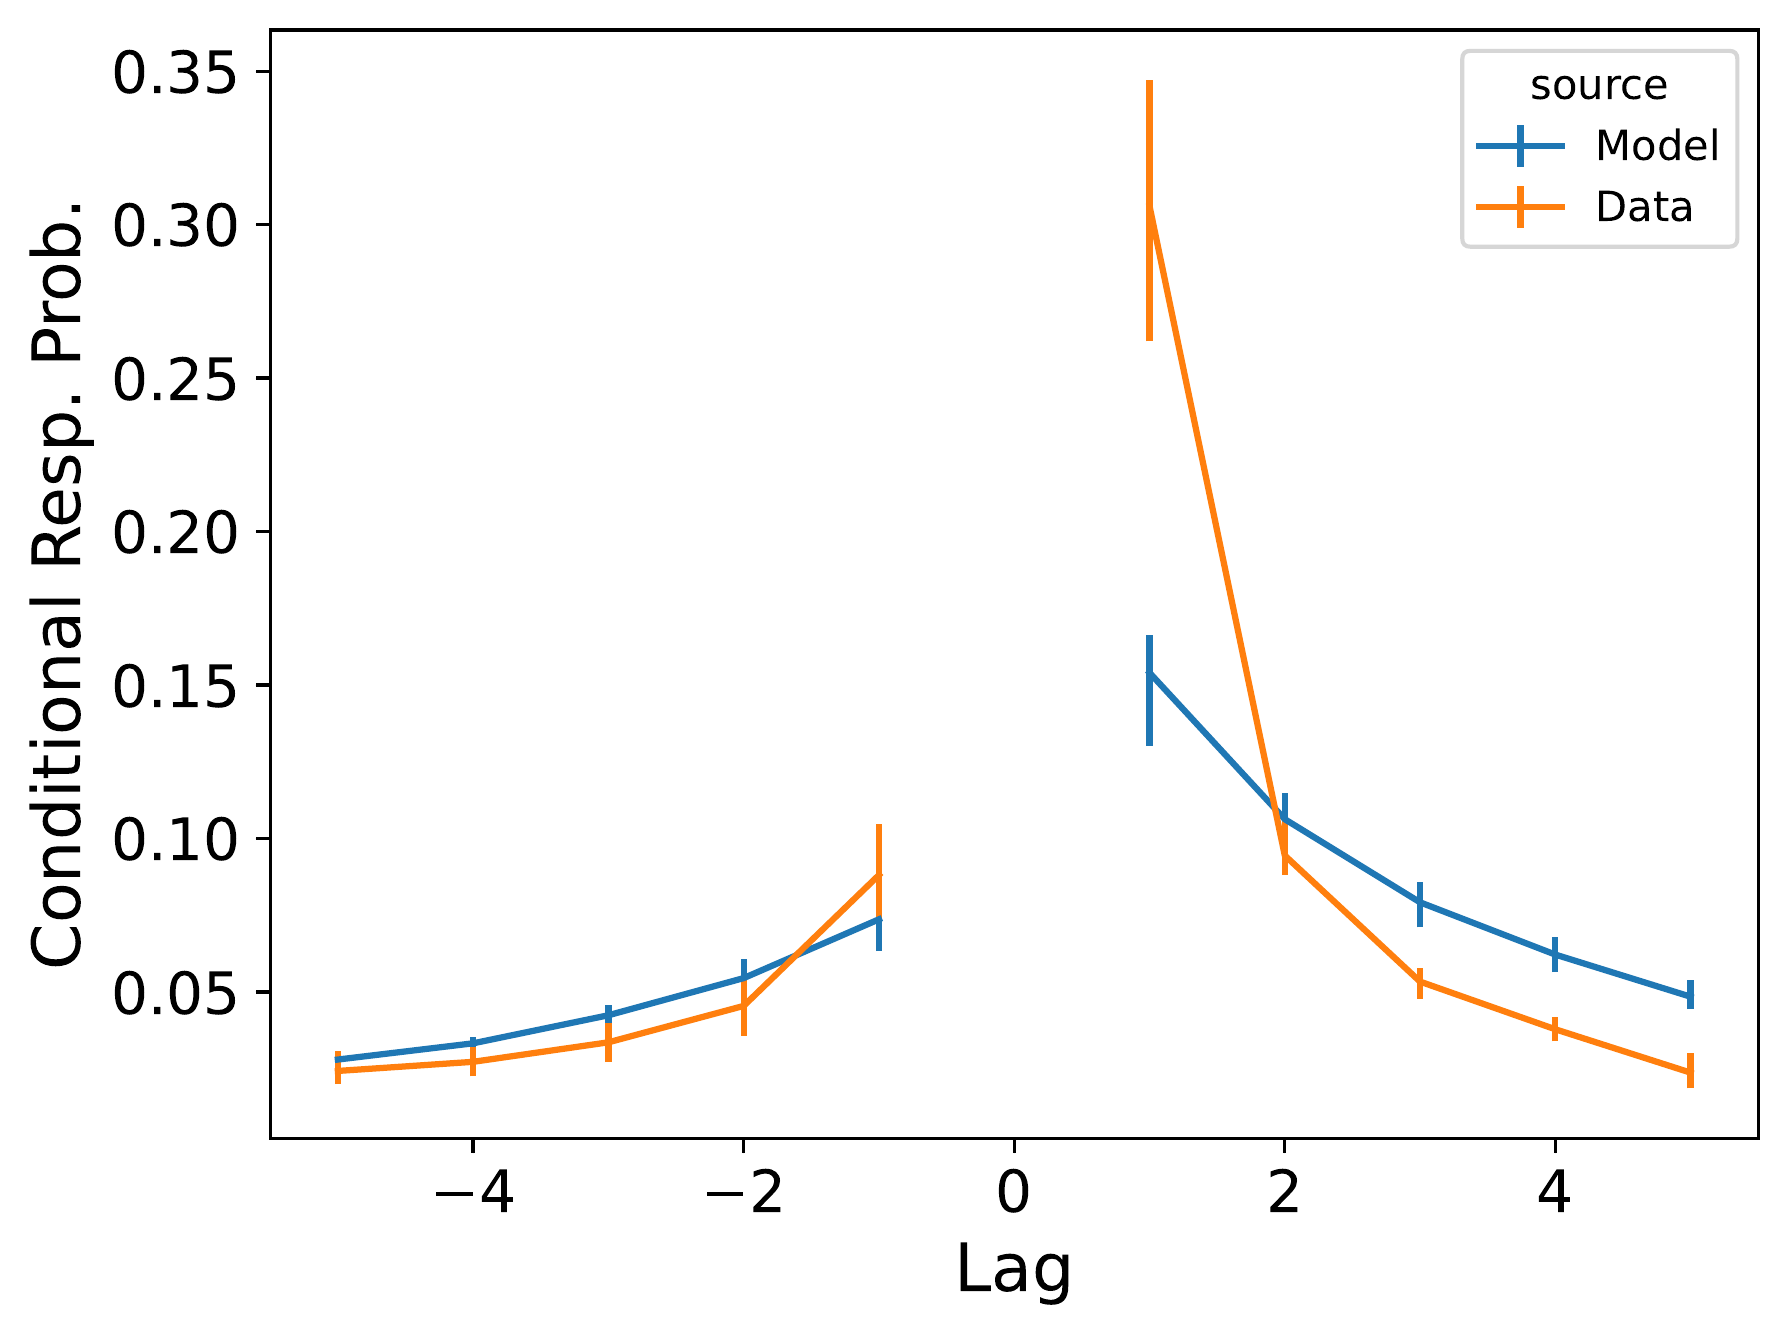
\includegraphics{icmr_figures/Murdock1962_InstanceCMR_Model_Fitting_LL40_crp-1.png}\end{minipage}%
%
\begin{minipage}{0.33\linewidth}
\includegraphics{icmr_figures/Murdock1962_InstanceCMR_Model_Fitting_LL40_pnr-1.png}\end{minipage}%
%
\begin{minipage}{0.33\linewidth}
\includegraphics{icmr_figures/Murdock1962_InstanceCMR_Model_Fitting_LL40_spc-1.png}\end{minipage}%
\newline
\begin{minipage}{0.33\linewidth}
\includegraphics{icmr_figures/Murdock1962_TraceScalingCMR_Model_Fitting_LL40_crp-1.png}\end{minipage}%
%
\begin{minipage}{0.33\linewidth}
\includegraphics{icmr_figures/Murdock1962_TraceScalingCMR_Model_Fitting_LL40_pnr-1.png}\end{minipage}%
%
\begin{minipage}{0.33\linewidth}
\includegraphics{icmr_figures/Murdock1962_TraceScalingCMR_Model_Fitting_LL40_spc-1.png}\end{minipage}%
\newline
\begin{minipage}{0.33\linewidth}
\includegraphics{icmr_figures/Murdock1962_MultiScalingCMR_Model_Fitting_LL40_crp-1.png}\end{minipage}%
%
\begin{minipage}{0.33\linewidth}
\includegraphics{icmr_figures/Murdock1962_MultiScalingCMR_Model_Fitting_LL40_pnr-1.png}\end{minipage}%
%
\begin{minipage}{0.33\linewidth}
\includegraphics{icmr_figures/Murdock1962_MultiScalingCMR_Model_Fitting_LL40_spc-1.png}\end{minipage}%

\caption{\label{fig-murdock1962memory40}Summary statistic fits to
Murdock Jr (1962) where list length = 40. Top: Connectionist CMR. Second
Row: Instance CMR, \(\tau_{t}\) set to 1. Third Row: Trace Scaling CMR
-- Instance CMR, \(\tau_{c}\) set to 1 and \(\tau_{t}\) optimized during
fitting. Fourth Row: Multi Scaling CMR -- Instance CMR, both \(\tau_t\)
and \(\tau_c\) freed for fitting. Left: conditional response probability
as a function of lag. Middle: probability of starting recall with each
serial position. Right: recall probability as a function of serial
position.}

\end{figure}%

\newpage{}

\subsubsection{Lohnas \& Kahana (2014)}\label{lohnas-kahana-2014}

\begin{longtable}[]{@{}
  >{\raggedright\arraybackslash}p{(\columnwidth - 10\tabcolsep) * \real{0.2800}}
  >{\raggedright\arraybackslash}p{(\columnwidth - 10\tabcolsep) * \real{0.1400}}
  >{\raggedright\arraybackslash}p{(\columnwidth - 10\tabcolsep) * \real{0.1400}}
  >{\raggedright\arraybackslash}p{(\columnwidth - 10\tabcolsep) * \real{0.1400}}
  >{\raggedright\arraybackslash}p{(\columnwidth - 10\tabcolsep) * \real{0.1400}}
  >{\raggedright\arraybackslash}p{(\columnwidth - 10\tabcolsep) * \real{0.1400}}@{}}
\caption{Confidence intervals of parameters fit to data from L. Lohnas
and Kahana (2014), computed across subjects. Column 1: Connectionist CMR
follows the specification in Morton and Polyn (2016). Second Row:
Instance CMR, with \(\tau_{t}\) set to 1. Third Row: Trace Scaling CMR
-- Instance CMR with \(\tau_{t}\) set to 1 and \(\tau_{c}\) optimized
during fitting. Fourth model Column 4: Instance CMR with both trace and
item activation scaling parameters freed for fitting.
}\label{tbl-lohnas}\tabularnewline
\toprule\noalign{}
\begin{minipage}[b]{\linewidth}\raggedright
\end{minipage} & \begin{minipage}[b]{\linewidth}\raggedright
Connectionist CMR
\end{minipage} & \begin{minipage}[b]{\linewidth}\raggedright
Instance CMR
\end{minipage} & \begin{minipage}[b]{\linewidth}\raggedright
Trace Scaling CMR
\end{minipage} & \begin{minipage}[b]{\linewidth}\raggedright
Multi Scaling CMR
\end{minipage} & \begin{minipage}[b]{\linewidth}\raggedright
\end{minipage} \\
\midrule\noalign{}
\endfirsthead
\toprule\noalign{}
\begin{minipage}[b]{\linewidth}\raggedright
\end{minipage} & \begin{minipage}[b]{\linewidth}\raggedright
Connectionist CMR
\end{minipage} & \begin{minipage}[b]{\linewidth}\raggedright
Instance CMR
\end{minipage} & \begin{minipage}[b]{\linewidth}\raggedright
Trace Scaling CMR
\end{minipage} & \begin{minipage}[b]{\linewidth}\raggedright
Multi Scaling CMR
\end{minipage} & \begin{minipage}[b]{\linewidth}\raggedright
\end{minipage} \\
\midrule\noalign{}
\endhead
\bottomrule\noalign{}
\endlastfoot
fitness & 1670.26 +/- 147.36 & 1672.85 +/- 147.45 & 1667.82 +/- 146.36 &
1669.93 +/- 148.38 & \\
encoding drift rate & 0.75 +/- 0.03 & 0.74 +/- 0.03 & 0.55 +/- 0.06 &
0.56 +/- 0.06 & \\
start drift rate & 0.58 +/- 0.11 & 0.59 +/- 0.10 & 0.56 +/- 0.08 & 0.61
+/- 0.07 & \\
recall drift rate & 0.95 +/- 0.02 & 0.95 +/- 0.01 & 0.90 +/- 0.02 & 0.90
+/- 0.02 & \\
shared support & 4.80 +/- 2.43 & 3.79 +/- 2.57 & 1.24 +/- 0.60 & 16.06
+/- 8.39 & \\
item support & 7.11 +/- 3.13 & 4.92 +/- 2.80 & 8.03 +/- 4.62 & 17.83 +/-
7.59 & \\
learning rate & 0.53 +/- 0.08 & 0.52 +/- 0.07 & 0.65 +/- 0.08 & 0.68 +/-
0.06 & \\
primacy scale & 11.89 +/- 7.78 & 9.45 +/- 7.12 & 14.54 +/- 5.55 & 7.43
+/- 4.31 & \\
primacy decay & 15.62 +/- 8.73 & 21.84 +/- 11.44 & 8.52 +/- 7.05 & 10.90
+/- 7.90 & \\
stop probability scale & 0.02 +/- 0.01 & 0.02 +/- 0.01 & 0.02 +/- 0.01 &
0.02 +/- 0.01 & \\
stop probability growth & 0.20 +/- 0.02 & 0.19 +/- 0.02 & 0.19 +/- 0.02
& 0.19 +/- 0.02 & \\
choice sensitivity & 21.39 +/- 11.06 & 15.15 +/- 9.67 & 1.00 +/- 0.00 &
19.32 +/- 10.90 & \\
mcf trace sensitivity & 1.00 +/- 0.00 & 1.00 +/- 0.00 & 3.44 +/- 0.42 &
2.76 +/- 0.43 & \\
\end{longtable}

\begin{figure}

\begin{minipage}{0.33\linewidth}
\includegraphics{icmr_figures/LohnasKahana2014_ConnectionistCMR_Model_Fitting_crp-1.png}\end{minipage}%
%
\begin{minipage}{0.33\linewidth}
\includegraphics{icmr_figures/LohnasKahana2014_ConnectionistCMR_Model_Fitting_pfr-1.png}\end{minipage}%
%
\begin{minipage}{0.33\linewidth}
\includegraphics{icmr_figures/LohnasKahana2014_ConnectionistCMR_Model_Fitting_spc-1.png}\end{minipage}%
\newline
\begin{minipage}{0.33\linewidth}
\includegraphics{icmr_figures/LohnasKahana2014_InstanceCMR_Model_Fitting_crp-1.png}\end{minipage}%
%
\begin{minipage}{0.33\linewidth}
\includegraphics{icmr_figures/LohnasKahana2014_InstanceCMR_Model_Fitting_pfr-1.png}\end{minipage}%
%
\begin{minipage}{0.33\linewidth}
\includegraphics{icmr_figures/LohnasKahana2014_InstanceCMR_Model_Fitting_spc-1.png}\end{minipage}%
\newline
\begin{minipage}{0.33\linewidth}
\includegraphics{icmr_figures/LohnasKahana2014_TraceScalingCMR_Model_Fitting_crp-1.png}\end{minipage}%
%
\begin{minipage}{0.33\linewidth}
\includegraphics{icmr_figures/LohnasKahana2014_TraceScalingCMR_Model_Fitting_pfr-1.png}\end{minipage}%
%
\begin{minipage}{0.33\linewidth}
\includegraphics{icmr_figures/LohnasKahana2014_TraceScalingCMR_Model_Fitting_spc-1.png}\end{minipage}%
\newline
\begin{minipage}{0.33\linewidth}
\includegraphics{icmr_figures/LohnasKahana2014_MultiScalingCMR_Model_Fitting_crp-1.png}\end{minipage}%
%
\begin{minipage}{0.33\linewidth}
\includegraphics{icmr_figures/LohnasKahana2014_MultiScalingCMR_Model_Fitting_pfr-1.png}\end{minipage}%
%
\begin{minipage}{0.33\linewidth}
\includegraphics{icmr_figures/LohnasKahana2014_MultiScalingCMR_Model_Fitting_spc-1.png}\end{minipage}%

\caption{\label{fig-lohnas2014memory}Summary statistic fits to L. Lohnas
and Kahana (2014). Top: Connectionist CMR. Second Row: Instance CMR,
\(\tau_{t}\) set to 1. Third Row: Trace Scaling CMR -- Instance CMR,
\(\tau_{c}\) set to 1 and \(\tau_{t}\) optimized during fitting. Fourth
Row: Multi Scaling CMR -- Instance CMR, both \(\tau_t\) and \(\tau_c\)
freed for fitting. Left: conditional response probability as a function
of lag. Middle: probability of starting recall with each serial
position. Right: recall probability as a function of serial position.}

\end{figure}%

Table~\ref{tbl-healey}, Table~\ref{tbl-murdock}, and
Table~\ref{tbl-lohnas} present the confidence intervals of the
parameters fit to the data across subjects for each model variant. The
tables also present the mean and confidence intervals of the
log-likelihood values for each model variant.
Figure~\ref{fig-healey2014memory}, Figure~\ref{fig-murdock1962memory20},
and Figure~\ref{fig-murdock1962memory30} illustrate the summary
statistic fits for each model variant. We additionally performed paired
t-tests to compare the log-likelihood values of the models across
subjects, using a significance level of \(0.05\) and Connectionist CMR
as the reference model. Alternative models Instance-CMR, Trace Scaling
CMR, and Multi Scaling CMR were compared to Connectionist CMR to
determine if subject-level log-likelihoods were significantly lower than
the reference model (lower scores indicate better fit), with outcome
p-values \textasciitilde0.0176, \textasciitilde0.0232, and
\textasciitilde0.0008, respectively. Performing the same tests for the
data from Murdock Jr (1962) yielded p-values 0.9125, 0.9414, and 0.6252
for the three alternative models, respectively. For the data from L.
Lohnas and Kahana (2014), the p-values were 0.8638, 0.1015, and 0.4374
for the three alternative models, respectively. These results suggest
that the Multi Scaling CMR model provides the best fit to the data
across all three datasets, with the Instance CMR model performing
similarly to the Connectionist CMR model. However, even the best-fitting
model, Multi Scaling CMR, only marginally outperforms Connectionist CMR
in terms of log-likelihood values and capture of summary statistics
across all datasets.

These several figures help illustrate a single point: the functional
equivalence between Connectionist and Instance CMR models. When the
trace-based activation scaling parameter \(\tau_{t}\) is set to 1, both
models yield the same results in free recall tasks, with differences in
results only attributable to the stochastic nature of the simulations
and fitting process. Even when \(\tau_{t}\) is varied during model
fitting, either instead of or in addition to the item activation scaling
parameter \(\tau_{c}\), model performance is only marginally different.
The challenges that the original Connectionist CMR faces in capturing
the dynamics of memory search in free recall tasks are shared by
Instance CMR, and are not clearly resolved by the latter model. For
example, both models overrate the strength of the lag-contiguity effect
in the dataset from Murdock Jr (1962), and lack the ability to capture
the plateau-like shape of the probability of first recall curve in data
both from Murdock Jr (1962) and L. Lohnas and Kahana (2014). These
results suggest that the instance-based specification of CMR does not
provide a clear advantage over the connectionist specification in terms
of capturing the dynamics of memory search in free recall tasks -- at
least not without additional modifications to the model or novel task
conditions.

\section{Discussion}\label{discussion}

In light of a collection of results across task domains distinguishing
between the performance of prototype- and instance-based models of
memory-based behavior, we searched for evidence of a similar distinction
with respect to the free recall task paradigm. To do this, we specified
and compared the original connectionist implementation of an established
model of task performance based in retrieved context theory
(Connectionist CMR) against a parallel instance-based variant (Instance
CMR) across diverse experimental conditions, including a dataset
featuring variable study list lengths across trials and a dataset
featuring item repetitions within trials and variable item repetition
spacing between trials. While our results identify some marginal
differences in model performance across datasets, they do not provide
clear evidence of a performance distinction between instance- and
instance-based models in the free recall task paradigm. The model
variants accounted for human performance on the free recall task with
similar effectiveness in each dataset considered. In addition, the
results of our semantic extension of Connectionist and Instance CMR
models will further underscore the portability of retrieved context
theory across model architectures. We show that the concatenation of
memory traces in a single memory structure is equivalent to a linear
combination of the separate retrieval of traces from two memory
structures, identify the mathematical basis for this equivalence, and
provide a foundation for future integrations of CMR with other cognitive
models.

Altogether these results demonstrate that the success of the theoretical
commitments made by the Context Maintenance and Retrieval (CMR) model
and models like it are likely not especially dependent on the
architectures in which they are implemented. Instead, the main insights
of retrieved context theories (at least as formalized by CMR) are highly
portable, and can likely be esconced within any reasonable model
architecture where memory search via temporal contextual representations
might prove valuable. Establishing the portability of these successful
theoretical principles across modeling approaches helps advance the
historical effort in cognitive science to develop ``a general account of
memory and its processes in a working computational system to produce a
common explanation of behavior rather than a set of lab-specific and
domain-specific theories for different behaviors'' (Newell 1973;
Jamieson et al. 2018).

An instance-based specification of CMR does not provide a clear
advantage over the connectionist specification in terms of capturing the
dynamics of memory search in free recall tasks -- at least not without
additional modifications to the model or novel task conditions. But a
few features unique to the instance-based specification of CMR may still
prove valuable in future research. Throughout this work, we emphasized
one of these: the instance-based specification of CMR is more easily
integrated with other instance-based models of memory, potentially
supporting lines of research that seek to combine the strengths of
different models to provide a more comprehensive account of memory
performance across different tasks.

Another feature of instance-based memory models that may prove valuable
in future research is their interpretability, the degree to which the
model's parameters and internal representations can be understood and
reasoned about (Gao and Guan 2023). Because instance models do not
compress information about the history of an item into a single vector,
they can be more easily interpreted than connectionist models. Each
trace is represented separately and its weighting in the activation
function is also calculated separately, making the contribution of each
trace to the model's output transparent in its internal structure. These
features may make instance-based models favorable for research that
seeks to diagnose and address the limitations of existing models, or to
develop new models that can capture the dynamics of memory search in
free recall tasks more effectively.

The most emphasized advantage of instance models in the literature
though is their ability to capture the dynamics of memory search in free
recall tasks more effectively than connectionist models via its use of
trace-based activation scaling in domains such as category learning and
semantic memory (Nosofsky and Zaki 2002; Jamieson et al. 2018). Why does
this advantage not appear when comparing Connectionist and Instance CMR
in the free recall task?

One key reason is that Connectionist CMR has some features that allow it
to exhibit instance-memory-like behavior in some aspects of its
dynamics. First, the item representations on its \(F\) layer are
orthonormal -- each item's representation is unique and does not overlap
with any other item's representation. This means that even without the
trace-based activation scaling unique to instance models, the model can
still selectively activate the representation of a single item in the
\(F\) layer without activating the representations of other items,
making Instance \(M^{FC}\) and Connectionist \(M^{FC}\) equivalent for
all values of \(\tau_{t}\). Similarities between \(\tau_{t}\) in the
instance-based model and \(\tau_{c}\) in the connectionist model also
contribute to the similarity in model performance. Despite some
fundamental differences, both activation scaling mechanisms help to
focus the model's attention on the most relevant traces in memory,
perhaps enough to in a broad range of cases obscure the differences in
model performance that might be expected from the different
architectures.

A more fundamental issue for comparison between Instance and
Connectionist CMR is that the free recall task and design of CMR might
not instantiate a clear instance vs prototype model distinction that has
set up previous successes of instance models in other domains. In these
other domains, experiments were configured to support clear contrasts
between prototype-based decision-making where the central tendency of a
class drives responses, and instance-based decision-making where the the
similarity of a probe to a specific study instance drives responses. The
free recall task is designed to test the ability of a model to retrieve
items from memory in a specific order, and the dynamics of memory search
in this task may not be as sensitive to the differences between instance
and prototype models as other tasks. However, future variations of the
task that introduce category structure as a major factor in recall, or
that require participants to make decisions based on the category
membership, might provide a clearer test of the distinction between
instance and prototype models in the domain of free recall. These
results highlight that the advantage of instance- over prototype- models
in accounting for memory performance is highly contingent on the task
and conditions under which models are tested.

\bookmarksetup{startatroot}

\chapter*{References}\label{references}
\addcontentsline{toc}{chapter}{References}

\markboth{References}{References}

\phantomsection\label{refs}
\begin{CSLReferences}{1}{0}
\bibitem[\citeproctext]{ref-anderson1995introduction}
Anderson, James A. 1995. \emph{An Introduction to Neural Networks}. MIT
press.

\bibitem[\citeproctext]{ref-cox2020similarity}
Cox, Gregory E, and Amy H Criss. 2020. {``Similarity Leads to Correlated
Processing: A Dynamic Model of Encoding and Recognition of Episodic
Associations.''} \emph{Psychological Review} 127 (5): 792.

\bibitem[\citeproctext]{ref-friendly1982toronto}
Friendly, Michael, Patricia E Franklin, David Hoffman, and David C
Rubin. 1982. {``The Toronto Word Pool: Norms for Imagery, Concreteness,
Orthographic Variables, and Grammatical Usage for 1,080 Words.''}
\emph{Behavior Research Methods \& Instrumentation} 14 (4): 375--99.

\bibitem[\citeproctext]{ref-gao2023interpretability}
Gao, Lei, and Ling Guan. 2023. {``Interpretability of Machine Learning:
Recent Advances and Future Prospects.''} \emph{IEEE MultiMedia} 30 (4):
105--18.

\bibitem[\citeproctext]{ref-griffiths2007topics}
Griffiths, Thomas L, Mark Steyvers, and Joshua B Tenenbaum. 2007.
{``Topics in Semantic Representation.''} \emph{Psychological Review} 114
(2): 211.

\bibitem[\citeproctext]{ref-healey2014memory}
Healey, M Karl, and Michael J Kahana. 2014. {``Is Memory Search Governed
by Universal Principles or Idiosyncratic Strategies?''} \emph{Journal of
Experimental Psychology: General} 143 (2): 575.

\bibitem[\citeproctext]{ref-healey2016four}
---------. 2016. {``A Four-Component Model of Age-Related Memory
Change.''} \emph{Psychological Review} 123 (1): 23.

\bibitem[\citeproctext]{ref-healey2019contiguity}
Healey, M Karl, Nicole M Long, and Michael J Kahana. 2019. {``Contiguity
in Episodic Memory.''} \emph{Psychonomic Bulletin \& Review} 26 (3):
699--720.

\bibitem[\citeproctext]{ref-hebb1949organization}
Hebb, Donald O. 1949. {``Organization of Behavior. New York: Wiley.''}
\emph{J. Clin. Psychol} 6 (3): 335--07.

\bibitem[\citeproctext]{ref-henson1996unchained}
Henson, Richard NA. 1996. {``Unchained Memory: Error Patterns Rule Out
Chaining Models of Immediate Serial Recall.''} \emph{The Quarterly
Journal of Experimental Psychology Section A} 49 (1): 80--115.

\bibitem[\citeproctext]{ref-hintzman1984minerva}
Hintzman, Douglas L. 1984. {``MINERVA 2: A Simulation Model of Human
Memory.''} \emph{Behavior Research Methods, Instruments, \& Computers}
16 (2): 96--101.

\bibitem[\citeproctext]{ref-hintzman1986schema}
---------. 1986. {``" Schema Abstraction" in a Multiple-Trace Memory
Model.''} \emph{Psychological Review} 93 (4): 411.

\bibitem[\citeproctext]{ref-hintzman1988judgments}
---------. 1988. {``Judgments of Frequency and Recognition Memory in a
Multiple-Trace Memory Model.''} \emph{Psychological Review} 95 (4): 528.

\bibitem[\citeproctext]{ref-homa1981limitations}
Homa, Donald, Sharon Sterling, and Lawrence Trepel. 1981. {``Limitations
of Exemplar-Based Generalization and the Abstraction of Categorical
Information.''} \emph{Journal of Experimental Psychology: Human Learning
and Memory} 7 (6): 418.

\bibitem[\citeproctext]{ref-howard2002distributed}
Howard, Marc W, and Michael J Kahana. 2002. {``A Distributed
Representation of Temporal Context.''} \emph{Journal of Mathematical
Psychology} 46 (3): 269--99.

\bibitem[\citeproctext]{ref-jamieson2018instance}
Jamieson, Randall K, Johnathan E Avery, Brendan T Johns, and Michael N
Jones. 2018. {``An Instance Theory of Semantic Memory.''}
\emph{Computational Brain \& Behavior} 1: 119--36.

\bibitem[\citeproctext]{ref-kahana1996associative}
Kahana, Michael J. 1996. {``Associative Retrieval Processes in Free
Recall.''} \emph{Memory \& Cognition} 24 (1): 103--9.

\bibitem[\citeproctext]{ref-kahana2020computational}
---------. 2020. {``Computational Models of Memory Search.''}
\emph{Annual Review of Psychology} 71: 107--38.

\bibitem[\citeproctext]{ref-kahana2000interresponse}
Kahana, Michael J, and Joshua Jacobs. 2000. {``Interresponse Times in
Serial Recall: Effects of Intraserial Repetition.''} \emph{Journal of
Experimental Psychology: Learning, Memory, and Cognition} 26 (5): 1188.

\bibitem[\citeproctext]{ref-kelly2017memory}
Kelly, Mary Alexandria, Douglas JK Mewhort, and Robert L West. 2017.
{``The Memory Tesseract: Mathematical Equivalence Between Composite and
Separate Storage Memory Models.''} \emph{Journal of Mathematical
Psychology} 77: 142--55.

\bibitem[\citeproctext]{ref-kragel2015neural}
Kragel, James E, Neal W Morton, and Sean M Polyn. 2015. {``Neural
Activity in the Medial Temporal Lobe Reveals the Fidelity of Mental Time
Travel.''} \emph{Journal of Neuroscience} 35 (7): 2914--26.

\bibitem[\citeproctext]{ref-logan2018automatic}
Logan, Gordon D. 2018. {``Automatic Control: How Experts Act Without
Thinking.''} \emph{Psychological Review} 125 (4): 453.

\bibitem[\citeproctext]{ref-logan2021serial}
---------. 2021. {``Serial Order in Perception, Memory, and Action.''}
\emph{Psychological Review} 128 (1): 1.

\bibitem[\citeproctext]{ref-lohnas2024retrieved}
Lohnas, Lynn J. 2024. {``A Retrieved Context Model of Serial Recall and
Free Recall.''} \emph{Computational Brain \& Behavior}, 1--35.

\bibitem[\citeproctext]{ref-lohnas2015expanding}
Lohnas, Lynn J, Sean M Polyn, and Michael J Kahana. 2015. {``Expanding
the Scope of Memory Search: Modeling Intralist and Interlist Effects in
Free Recall.''} \emph{Psychological Review} 122 (2): 337.

\bibitem[\citeproctext]{ref-lohnas2014retrieved}
Lohnas, Lynn, and Michael J Kahana. 2014. {``A Retrieved Context Account
of Spacing and Repetition Effects in Free Recall.''} \emph{Journal of
Experimental Psychology: Learning, Memory, and Cognition} 40 (3): 755.

\bibitem[\citeproctext]{ref-morton2016predictive}
Morton, Neal W, and Sean M Polyn. 2016. {``A Predictive Framework for
Evaluating Models of Semantic Organization in Free Recall.''}
\emph{Journal of Memory and Language} 86: 119--40.

\bibitem[\citeproctext]{ref-murdock1962serial}
Murdock Jr, Bennet B. 1962. {``The Serial Position Effect of Free
Recall.''} \emph{Journal of Experimental Psychology} 64 (5): 482.

\bibitem[\citeproctext]{ref-newell1973you}
Newell, Allen. 1973. {``You Can't Play 20 Questions with Nature and Win:
Projective Comments on the Papers of This Symposium.''} In \emph{Machine
Intelligence}, 121--46. Routledge.

\bibitem[\citeproctext]{ref-nosofsky2002exemplar}
Nosofsky, Robert M, and Safa R Zaki. 2002. {``Exemplar and Prototype
Models Revisited: Response Strategies, Selective Attention, and Stimulus
Generalization.''} \emph{Journal of Experimental Psychology: Learning,
Memory, and Cognition} 28 (5): 924.

\bibitem[\citeproctext]{ref-polyn2009context}
Polyn, Sean M, Kenneth A Norman, and Michael J Kahana. 2009. {``A
Context Maintenance and Retrieval Model of Organizational Processes in
Free Recall.''} \emph{Psychological Review} 116 (1): 129.

\bibitem[\citeproctext]{ref-ramsauer2020hopfield}
Ramsauer, Hubert, Bernhard Schäfl, Johannes Lehner, Philipp Seidl,
Michael Widrich, Thomas Adler, Lukas Gruber, et al. 2020. {``Hopfield
Networks Is All You Need.''} \emph{arXiv Preprint arXiv:2008.02217}.

\bibitem[\citeproctext]{ref-shiffrin1997model}
Shiffrin, Richard M, and Mark Steyvers. 1997. {``A Model for Recognition
Memory: REM---Retrieving Effectively from Memory.''} \emph{Psychonomic
Bulletin \& Review} 4: 145--66.

\bibitem[\citeproctext]{ref-siegel2014retrieved}
Siegel, Lynn L, and Michael J Kahana. 2014. {``A Retrieved Context
Account of Spacing and Repetition Effects in Free Recall.''}
\emph{Journal of Experimental Psychology: Learning, Memory, and
Cognition} 40 (3): 755.

\bibitem[\citeproctext]{ref-stanton2002comparisons}
Stanton, Roger D, Robert M Nosofsky, and Safa R Zaki. 2002.
{``Comparisons Between Exemplar Similarity and Mixed Prototype Models
Using a Linearly Separable Category Structure.''} \emph{Memory \&
Cognition} 30 (6): 934--44.

\bibitem[\citeproctext]{ref-steyvers2005word}
Steyvers, Mark, Richard M Shiffrin, and Douglas L Nelson. 2005. {``Word
Association Spaces for Predicting Semantic Similarity Effects in
Episodic Memory.''}

\bibitem[\citeproctext]{ref-storn1997differential}
Storn, Rainer, and Kenneth Price. 1997. {``Differential Evolution--a
Simple and Efficient Heuristic for Global Optimization over Continuous
Spaces.''} \emph{Journal of Global Optimization} 11 (4): 341--59.

\bibitem[\citeproctext]{ref-talmi2019retrieved}
Talmi, Deborah, Lynn J Lohnas, and Nathaniel D Daw. 2019. {``A Retrieved
Context Model of the Emotional Modulation of Memory.''}
\emph{Psychological Review} 126 (4): 455.

\bibitem[\citeproctext]{ref-turner2019toward}
Turner, Brandon M. 2019. {``Toward a Common Representational Framework
for Adaptation.''} \emph{Psychological Review} 126 (5): 660.

\bibitem[\citeproctext]{ref-wachter2019retrieved}
Wachter, Jessica A, and Michael Jacob Kahana. 2019. {``A
Retrieved-Context Theory of Financial Decisions.''} National Bureau of
Economic Research.

\end{CSLReferences}




\end{document}
